\documentclass[12pt]{article}
\usepackage{html}
\usepackage{url}
\usepackage{booktabs}
\usepackage{color}
\usepackage{verbatim}
\usepackage{upquote}
\usepackage{fancyvrb}
\usepackage{xspace}
\usepackage{amsmath}
\usepackage{amssymb}
\usepackage{hyperref}
\usepackage{longtable}
\usepackage{colortbl}
\usepackage{bm}
\usepackage{lscape}
\usepackage{amsmath}
\usepackage{pdfpages}

% textcomp for those distros without builtin \textquotesingle (macros.tex)
\usepackage{textcomp}
\setlength{\textheight}{9in}
\setlength{\textwidth}{6.5in}
\setlength{\hoffset}{0in}
\setlength{\voffset}{0in}
\setlength{\headheight}{0in}
\setlength{\headsep}{0in}
\setlength{\topmargin}{0in}
\setlength{\oddsidemargin}{-0.05in}
\setlength{\evensidemargin}{-0.05in}
\setlength{\marginparsep}{0in}
\setlength{\marginparwidth}{0in}
\setlength{\parsep}{0.8ex}
\setlength{\parskip}{1ex plus \fill}
\baselineskip 18pt
\renewcommand{\topfraction}{.8}
\renewcommand{\bottomfraction}{.2}

\makeatletter
\renewcommand\paragraph{\@startsection {paragraph}{4}{\z@}%
                                   {-3.5ex \@plus -1ex \@minus -.2ex}%
                                   {0.3ex \@plus.2ex}%
                                   {\normalfont\footnotesize\mdseries}}
\makeatother


%%%%%%%%%%%%%%%%%%%%%%%
% Start document
%%%%%%%%%%%%%%%%%%%%%%%
\setcounter{page}{1}
\begin{document}

%%%%%%%%%%%%%%%%%%%%%%%
% Definitions
%%%%%%%%%%%%%%%%%%%%%%%

\newcommand{\PSI}{{\tt PSI}}
\newcommand{\PSItwo}{{\tt PSI2}}
\newcommand{\PSIthree}{{\tt PSI3}}
\newcommand{\PSIfour}{{\tt PSI4}}
\newcommand{\PSIversion}{4.0.0-alpha}
\newcommand{\PSImmmversion}{4.0.0-alpha}
\newcommand{\PSIemail}{psicode@users.sourceforge.net}

%
% Psi Modules
%
\def\module#1{{\tt #1}}
\newcommand{\libmints}{\module{libmints}}
\newcommand{\PSIdriver}{\module{psi4}}
\newcommand{\PSIinput}{\module{input}}
\newcommand{\PSIcints}{\module{cints}}
\newcommand{\PSIcderiv}{\module{cints --deriv1}}
\newcommand{\PSIdetci}{\module{detci}}
\newcommand{\PSIdetcas}{\module{detcas}}
\newcommand{\PSIdetcasman}{\module{detcasman}}
\newcommand{\PSIclag}{\module{clag}}
\newcommand{\PSIccenergy}{\module{ccenergy}}
\newcommand{\PSIccsort}{\module{ccsort}}
\newcommand{\PSIpsi}{\module{psi}}
\newcommand{\PSIcscf}{\module{cscf}}
\newcommand{\PSIoptking}{\module{optking}}
\newcommand{\PSItransqt}{\module{transqt}}
\newcommand{\PSInormco}{\module{normco}}
\newcommand{\PSIintder}{\module{intder95}}
\newcommand{\PSIgeom}{\module{geom}}
\newcommand{\PSIoeprop}{\module{oeprop}}
\newcommand{\PSIstable}{\module{stable}}

%
% Psi Library
%
\def\library#1{{\tt #1}}

%
% Psi and Unix Files
%
\def\FILE#1{{\tt file#1}}
\def\file#1{{\tt #1}}
\newcommand{\chkptfile}{\file{file32}}
\newcommand{\inputdat}{\file{input.dat}}
\newcommand{\outputdat}{\file{output.dat}}
\newcommand{\fconstdat}{\file{fconst.dat}}
\newcommand{\intcodat}{\file{intco.dat}}
\newcommand{\optaux}{\file{opt.aux}}
\newcommand{\basisdat}{\file{basis.dat}}
\newcommand{\pbasisdat}{\file{pbasis.dat}}
\newcommand{\geomdat}{\file{geom.dat}}
\newcommand{\geomout}{\file{geom.out}}

%
% Psi Keywords
%
\def\keyword#1{{\tt #1}}

%
% Psi C and Fortran Language elements
%
\def\celem#1{{\tt #1}}
\def\felem#1{{\tt #1}}

%
% Unix stuff
%
\def\unixid#1{{\em #1}} % names of groups and users
\def\shellvar#1{{\tt #1}}

%
% Nice output for function description
%
% Needs 4 arguments: function declaration,
%  description, arguments, and return values
%
% Call \initfuncdesc before using \funcdesc
%
\newcommand{\initfuncdesc}
{\newlength{\lcwidth}
\settowidth{\lcwidth}{Arguments:}
\newlength{\rcwidth}
\setlength{\rcwidth}{\linewidth}
\addtolength{\rcwidth}{-1.0\lcwidth}
\addtolength{\rcwidth}{-6.0\tabcolsep}
}

\newcommand{\funcdesc}[4]{
\celem{#1} \\
#2

\begin{tabular}{lp{\rcwidth}}
Arguments: & #3\\
Returns: & #4
\end{tabular}}

% This allows us to read in a sample file, needs the listings package
\newcommand \includesource[2] {
   \definecolor{XCodeComment}{rgb}{0.0, 0.4531, 0.0}
   \definecolor{XCodeKeyword}{rgb}{0.6641, 0.0508, 0.5664}
   \definecolor{XCodeString}{rgb}{0.7656, 0.1016, 0.0859}
   \lstset{
      language={#2}, basicstyle= \slshape \scriptsize \ttfamily,
      keywordstyle= \color{XCodeKeyword}, identifierstyle= \slshape \scriptsize,
      commentstyle= \color{XCodeComment},
      stringstyle=\ttfamily \color{XCodeString},
      showstringspaces=false,
      numbers=left,
      tabsize=4,
      title=\textit{#1},
      breaklines=true,
      showspaces=false,
      showtabs=false, frame=tb, framerule=0.5mm,
      aboveskip=5mm, belowskip=5mm,
   }
   \lstinputlisting{#1}
}

\newcommand \includeinput[1]{
   \lstdefinelanguage{psi}{
           morekeywords={geometry,label,wfn,refernce,subgroup,basis,docc,
                         print,do\_tei,ri\_basis,zmat,psi, reference,
                         df-mp2},
           sensitive=false,
           morecomment=[l]{\%}
   }
   \includesource{#1}{psi}
}


\title{The \PSIfour User's Manual}
\date{Created on: \today}
%
% People who contributed to the writing of this manual (may be a different
% set of people than those who contributed to the code).  Please add
% yourself if we forgot anyone -CDS
%
\author{
Andrew C.\ Simmonett
\and Robert M.\ Parrish
\and Lori A. Burns
\and Edward G.\ Hohenstein
\and Masaaki Saitow
\and Justin M.\ Turney
\and Rollin A.\ King
\and T.\ Daniel Crawford
\and C.\ David Sherrill}

\maketitle

\PSIfour\ Version: \PSIversion \\
Report bugs to: \PSIemail \\

\thispagestyle{empty}

\newpage
\tableofcontents
\newpage

The purpose of this manual is to provide a reasonably detailed
overview of the source code and programming philosophy of \PSIfour,
such that programmers interested in contributing to the code will have
an easier task.  Section \ref{svn} gives a succint explanation of the
steps required to obtain the source code from the main repository at
Virginia Tech.  (Installation instructions are given separately in the
installation manual or in \$PSI4/INSTALL.) \ref{Style} offers advice on
appropriate programming style for \PSIfour\ code, and section \ref{Makefiles}
describes the structure of the package's \file{Makefile}s.  Section
The appendices provide important reference material,
including the currently accepted \PSIfour\ citation and format
information for some of the most important text files used by
\PSIfour\ modules.

There are many examples included in this document to provide sample input files
and source files; these can be found in ASCII form in the \PSIfour\ source
itself.  Each included file has a path, which is relative to
\$PSI4/doc/progman, as its title and this is where the unformatted file can be
found.  The examples described herein can even be compiled from the directories
in which the source files are found.

\section{A \PSIfour\ Tutorial} \label{sec:tutorial}

\subsection{Basic Input File Structure}

PSI4 reads input from a text file, which can be prepared in any standard
text editor.  The default input file name is \file{input.dat} and the
default output file name is \file{output.dat}.  So that you can give your
files meaningful names, these defaults can be changed by specifying
the input file name and output file name on the the command line.
The syntax is:

{\tt psi4 input-name output-name}

\subsection{Running a Basic Hartree--Fock Calculation}
In our first example, we will consider a Hartree--Fock SCF computation
for the water molecule using a cc-pVDZ basis set.  We will specify the
geometry of our water molecule using a standard Z-matrix.

\begin{Snippet}

# Any line starting with the # character is a comment line
# Here's a sample HF/cc-pVDZ H2O computation

molecule h2o {
  O
  H 1 0.96
  H 1 0.96 2 104.5
}

set basis cc-pVDZ
energy('scf')
\end{Snippet}

For your convenience, this example can be found in {\tt
psi4/samples/tu1-h2o-energy/input.dat}.  You can run it if you wish.
Once \PSIfour\ is in your path (see the User Configuration section of
the installation instructions), you can run this computation by typing
\begin{verbatim}
psi4 input.dat output.dat
\end{verbatim}
If everything goes well, the computation should complete and should report
a final restricted Hartree--Fock energy in a section like this:
\begin{verbatim}
  Energy converged.

  @RHF Final Energy:   -76.02665366589162
\end{verbatim}
By default, the energy should be converged to about 1.0\e{-8}, so agreement
is only expected for about the first 8 digits after the decimal.  If the
computation does not complete, there is probably a problem with the
compilation or installation of the program (see the installation
instructions in Sec. \ref{sec:installation}).

This very simple input is sufficient to run the requested information.
Notice that we didn't tell the program some otherwise useful information
like the charge on the molecule (0, it's neutral), the spin multiplicity
(1 for a closed-shell molecule with all electrons paired), or the reference
wavefunction to use (restricted Hartree--Fock, or RHF, is usually
appropriate for a closed-shell molecule).  The program correctly guessed
all of these options for us.  We can change the default behavior through
additional keywords.

Let's consider what we would do for an open-shell molecule, where
not all electrons are paired.  For example, let's run a computation
on methylene (CH$_2$), whose ground electronic state has two unpaired
electrons (triplet electronic state, or a spin multiplicity $2S+1 = 3$).
In this case, the default spin multiplicity (1) is not correct, so we
need to tell the program the true value (3).  Like many programs, \PSIfour\
can get the charge and multiplicity as the first two integers in the
Z-matrix.  Note the line with {\tt 0 3} at the beginning of the molecule
specification below.  In this example we will also specify the bond length
and bond angle as variables ({\tt R} and {\tt A}), whose values are given
at the end of the Z-matrix specification.

\begin{Snippet}
# Here's a sample UHF/6-31G** CH2 computation

molecule ch2 {
  0 3
  C
  H 1 R
  H 1 R 2 A

  R = 1.075
  A = 133.93
}

set basis 6-31G**
set reference uhf

energy ('scf')
\end{Snippet}

This sample input can be found in {\tt psi4/samples/tu2-ch2-energy}, and as
before it can be run through the command {\tt psi4 input.dat output.dat}
(actually, because {\tt psi4} by default looks for an input file named {\tt
input.dat} and writes by default to a file called {\tt output.dat}, in this
case one could also just type {\tt psi4}).  If it works, it should print
the final energy as
\begin{verbatim}
  @UHF Final Energy:   -38.92534160932308
\end{verbatim}
Notice we added a new keyword, {\tt set reference uhf}, to the input.  For
open-shell molecules, we have a choice of unrestricted orbitals
(unrestricted Hartree--Fock, or UHF), or restricted orbitals (restricted
open-shell Hartree--Fock, or ROHF).  Usually, UHF is a little easier to
converge (although it may be more susceptible to spin contamination than
ROHF).

\subsection{Geometry Optimization and Vibrational Frequency Analysis}
The above examples were simple single-point energy computations
(as specified by the {\tt energy()} function).  Of course there are other
kinds of computations to perform, such as geometry optimizations and
vibrational frequency computations.  These can be specified by replacing
{\tt energy()} with {\tt optimize()} or {\tt frequencies()}, respectively.

Here's an example of optimizing the H$_2$O molecule using Hartree--Fock with
a cc-pVDZ basis set (located in {\tt psi4/samples/tu3-h2o-opt}).
\begin{Snippet}
# Optimize H2O HF/cc-pVDZ

molecule h2o {
  O
  H 1 0.96
  H 1 0.96 2 104.5
}

set basis cc-pVDZ
optimize('scf')
\end{Snippet}

This should perform a series of gradient computations.  The gradient points
which way is downhill in energy, and the optimizer then modifies the
geometry to follow the gradient.  After about 4 cycles, the geometry should
converge with a message like {\tt Optimization is complete!}.  As indicated
in the following table (printed by the optimizer at the end of the
computation), the energy decreases with each step,
and the maximum force on each atom also decreases with each step (in
principle these numbers could increase in some iterations, but here they do
not).

\begin{Snippet}
----------------------------------------------------------------------
Step         Energy             Delta(E)      MAX force   MAX Delta(q)
----------------------------------------------------------------------
  1    -76.026653665892    -76.026653665892    1.52e-02   1.52e-02
  2    -76.026907793199     -0.000254127307    9.55e-03   9.55e-03
  3    -76.027052927171     -0.000145133972    4.47e-04   4.47e-04
  4    -76.027053472137     -0.000000544965    1.16e-04   1.16e-04
----------------------------------------------------------------------
\end{Snippet}

To get harmonic vibrational frequencies, {\em first we must set up an input
using the OPTIMIZED GEOMETRY}.  We can easily get the optimized geometry
from the previous computation.  Looking at the output from running the
previous example, we see that the OH bond length is about 0.9463 {\AA}ngstroms,
and the bond angle is about 104.575 degrees.  It's good to give this many
digits (or more) to make sure there's not significant roundoff error in the
geometry when running a frequency computation.  So, our frequency
computation input (which can be found as test case {\tt
psi4/samples/tu4-h2o-freq}) is:
\begin{Snippet}
# Frequencies for H2O HF/cc-pVDZ at optimized geometry

molecule h2o {
  O
  H 1 0.9463
  H 1 0.9463 2 104.575
}

set basis cc-pVDZ
frequencies('scf')
\end{Snippet}
Alternatively, it's also possible for \PSIfour\ to use Cartesian coordinate
input.  Here, the Cartesian coordinates of the optimized geometry can be
extracted from the {\em bottom} of the optimization output.  The input
would then look like
this:
\begin{Snippet}
molecule h2o {
  O     0.0000000000  -0.0000000000  -0.1224239500
  H     0.0000000000  -1.4147069876   0.9714784639
  H    -0.0000000000   1.4147069876   0.9714784639
}

set basis cc-pVDZ
frequencies('scf')
\end{Snippet}
If either of the inputs above are run, the program should do some
computations and then finally report the following harmonic vibrational
frequencies (roundoff errors of around 0.1 cm$^{-1}$ may exist):
\begin{Snippet}
          Irrep      Harmonic Frequency
                          (cm-1)
        -----------------------------------------------
             A1         1776.1735
             A1         4113.8031
             B2         4211.7879
        -----------------------------------------------
\end{Snippet}
Notice that the symmetry type of the normal modes is specified (A1, A1,
B2).  The program also prints out the normal modes in terms of Cartesian
coordinates of each atom.  For example, the normal mode at 1776 cm$^{-1}$
is
\begin{Snippet}
   Frequency:       1776.17
   Force constant:   0.1194
             X       Y       Z
  O        0.000   0.000  -0.067
  H        0.000   0.416   0.536
  H        0.000  -0.416   0.536
\end{Snippet}
where the table shows the displacements in the X, Y, and Z dimensions for
each atom along the normal mode coordinate.  (This information could be used
to animate the vibrational frequency using visualization software.)


\subsection{Analysis of Intermolecular Interactions}
Now let's consider something a little more interesting.  \PSIfour\
contains code to analyze the nature of intermolecular interactions
between two molecules, via symmetry-adapted perturbation theory
(SAPT) \cite{Jeziorski:1994:1887}.  This kind of analysis gives a lot
of insight into the nature of intermolecular interactions, and \PSIfour\
makes these computations easier than ever.

For a SAPT computation, the input needs to provide information on two
distinct molecules.  This is very easy, we just give a Z-matrix or set of
Cartesian coordinates for each molecule, and separate the two with two
dashes, like this:
\begin{Snippet}
# Example SAPT computation for ethene*ethine (i.e., ethylene*acetylene),
# test case 16 from the S22 database

molecule dimer {
0 1
C   0.000000  -0.667578  -2.124659
C   0.000000   0.667578  -2.124659
H   0.923621  -1.232253  -2.126185
H  -0.923621  -1.232253  -2.126185
H  -0.923621   1.232253  -2.126185
H   0.923621   1.232253  -2.126185
--
0 1
C   0.000000   0.000000   2.900503
C   0.000000   0.000000   1.693240
H   0.000000   0.000000   0.627352
H   0.000000   0.000000   3.963929
units angstrom

no_reorient
symmetry c1
}
\end{Snippet}

Notice we have a couple of new keywords in the molecule specification.
{\tt no\_reorient} tells the program not to reorient the molecule
to a different coordinate system (this is important for SAPT to make
sure the same coordinate frame is used for the computations of the two
monomers and for the dimer).  The next keyword tells \PSIfour\ to run
in C1 point-group symmetry (i.e., without using symmetry), even if a
higher symmetry is detected.  SAPT computations need to be run with
symmetry turned off in this way.

Here's the second half of the input:
\begin{Snippet}
set globals {
    basis jun-cc-pVDZ
    scf_type DF
    freeze_core True
}

energy('sapt0')
\end{Snippet}

Before, we have been setting keywords individually with commands like
{\tt set basis cc-pVDZ}.  Because we have a few more options now, it's
convenient to place them together into the {\tt set globals} or {\tt set}
block, bounded by {\tt \{\dots\}}.  This
will set all of these options as ``global'' options (meaning that they are
visible to all parts of the program).  Most common \PSIfour\ options can be
set in a {\tt globals} section like this.  If an option needs to be visible
only to one part of the program (e.g., we only want to increase the
energy convergence in the SCF code, but not the rest of the
code), it can be placed in a section of input visible to that part of the
program (e.g., {\tt set scf e\_convergence 1.0E-8}).

Back to our SAPT example, we have found that for basic-level SAPT
computations (i.e., SAPT0), a good error cancellation is found
\cite{Hohenstein:2012:WIREs} with the jun-cc-pVDZ basis (this is the
usual aug-cc-pVDZ basis, but without diffuse functions on hydrogen and
without diffuse $d$ functions on heavy atoms) \cite{Papajak:2011:10}. So,
we'll use that as our standard basis set.  The SAPT code is designed to
use density fitting techniques, because they introduce minimal errors
whil providing much faster computations \cite{Hohenstein:2010:184111,
Hohenstein:2010:014101}. Since we're using density fitting for the SAPT,
we might as well also use it for the Hartree--Fock computations that are
performed as part of the SAPT.  We can specify that with the option
and value pair \optionname{scf\_type} \optionval{df}.

Density fitting procedures require the use of auxiliary basis sets that
pair with the primary basis set.  Fortunately, \PSIfour\ is usually smart
enough to figure out what auxiliary basis sets are needed for a given
computation.  In this case, jun-cc-pVDZ is a standard enough basis set
(just a simple truncation of the very popular aug-cc-pVDZ basis set)
that \PSIfour\ correctly guesses that we want the jun-cc-pVDZ-JKFIT
auxiliary basis for the Hartree--Fock, and the jun-cc-pVDZ-RI basis set
for the SAPT procedure.

To speed up the computation a little, we also tell the SAPT procedure to
freeze the core electrons with the \optionname{freeze\_core} option.  The SAPT
procedure is invoked with the simple call, {\tt energy(\qq sapt0\qq)}.  This
call knows to automatically run two monomer computations and a dimer
computation and then use these results to perform the SAPT analysis.  The
various energy components are printed at the end of the output, in addition
to the total SAPT0 interaction energy.  An explanation of the various
energy components can be found in the review by Jeziorski, Moszynski, and
Szalewicz \cite{Jeziorski:1994:1887}, and this is discussed in more detail
in the SAPT section later in this manual.  For now, we'll note that most of
the SAPT energy components are negative; this means those are attractive
contributions (the zero of energy in a SAPT computation is defined as
non-interacting monomers).  The exchange contributions are positive
(repulsive).   In this example, the most attractive contribution between
ethylene and acetylene is an electrostatic term of $-2.12$ kcal mol$^{-1}$
({\tt Elst10,r} where the 1 indicates the first-order
perturbation theory result with respect to the intermolecular interaction,
and the 0 indicates zeroth-order with respect to intramolecular electron
correlation).  The next most attractive contribution is the {\tt Disp20}
term (2nd order intermolecular dispersion, which looks like an MP2 in which
one excitation is placed on each monomer), contributing an attraction of
$-1.21$ kcal mol$^{-1}$.  It is not surprising that the electrostatic
contribution is dominant, because the geometry chosen for this example has the
acetylene perpendicular to the ethylene, with the acetylene hydrogen
pointing directly at the double bond in ethylene; this will be attractive
because the H atoms in acetylene bear a partial positive charge, while the
electron-rich double bond in ethylene bears a partial negative charge.  At
the same time, the dispersion interaction should be smaller because the
perpendicular geometry does not allow much overlap between the monomers.
Hence, the SAPT analysis helps clarify (and quantify) our physical
understanding about the interaction between the two monomers.

\subsection{Potential Surface Scans and Counterpoise Correction Made Easy
with Psithon}

Finally, let's consider an example that shows how the Python driver
in \PSIfour\ simplifies some routine tasks.  \PSIfour\ can interpret
valid Python code in addition to the computational chemistry directives
we've seen in the previous examples; we call this mixture Psithon.
The Python computer language is very easy to pick up, and even users
previously unfamiliar with Python can use it to simplify tasks by
modifying some of the example input files supplied with \PSIfour\
in the {\tt psi4/samples} directory.

Suppose you want to do a limited potential energy surface scan, such as
computing the interaction energy between two neon atoms at various
interatomic distances.  One simple but unappealing way to do this is to
create separate input files for each distance to be studied.  But most of
these input files are identical, except that the interatomic distance is
different.  Psithon lets you specify all this in a single input file,
looping over the different distances with an array like this: {\tt
Rvals=[2.5, 3.0, 4.0]}.

Let's also suppose you want to do counterpoise (CP) corrected energies.
Counterpoise correction involves computing the dimer energy and then
subtracting out the energies of the two monomers, each evaluated in the
dimer basis.  Again, each of these computations could be run in a separate
input file, but because counterpoise correction is a fairly standard
procedure for intermolecular interactions, \PSIfour\ knows about it and has
a built-in routine to perform counterpoise correction.  It only needs to
know what method you want to do the counterpoise correction on (here, let's
consider CCSD(T)), and it needs to know what's monomer A and what's monomer
B.  This last issue of specifying the monomers separately was already dealt
with in the previous SAPT example, where we saw that two dashes in the {\tt
molecule} block can be used to separate monomers.

So, we're going to do counterpoise-corrected CCSD(T) energies for Ne$_2$ at
a series of different interatomic distances.  And let's print out a table
of the interatomic distances we've considered, and the CP-corrected CCSD(T)
interaction energies (in kcal mol$^{-1}$) at each geometry.  Doing all this
in a single input is surprisingly easy in \PSIfour.  Here's the input
(available as {\tt psi4/samples/tu6-cp-ne2}).

\begin{Snippet}
#! Example potential energy surface scan and CP-correction for Ne2

molecule dimer {
  Ne
--
  Ne 1 R
}

Rvals=[2.5, 3.0, 4.0]

set basis aug-cc-pVDZ
set freeze_core True

# Initialize a blank dictionary of counterpoise corrected energies
# (Need this for the syntax below to work)
ecp = {}

for R in Rvals:
  dimer.R = R
  ecp[R] = cp('ccsd(t)')

print "\n"
print "CP-corrected CCSD(T)/aug-cc-pVDZ interaction energies\n\n"
print "        R (Ang)         E_int (kcal/mol)             \n"
print "-----------------------------------------------------\n"
for R in Rvals:
  e = ecp[R] * psi_hartree2kcalmol
  print "        %3.1f            %10.6f\n" % (R, e)
\end{Snippet}

First, you can see the {\tt molecule} block has a couple dashes to
separate the monomers from each other.  Also note we've used a Z-matrix to
specify the geometry, and we've used a variable ({\tt R}) as the
interatomic distance.  We have {\em not} specified the value of {\tt R} in
the {\tt molecule} block like we normally would.  That's because we're
going to vary it during the scan across the potential energy surface.
Below the {\tt molecule} block, you can see the {\tt Rvals} array
specified.  This is a Python array holding the interatomic distances we
want to consider.  In Python, arrays are surrounded by square brackets, and
elements are separated by commas.

The next lines, {\tt set basis aug-cc-pVDZ} and {\tt set freeze\_core
True}, are familiar from previous test cases.  Next comes a slightly
unusual-looking line, {\tt ecp = \{\}}.  This is Python's way of initializing
a ``dictionary.''  We're going to use this dictionary to store the
counterpoise-corrected energies as they become available.  A dictionary is
like an array, but we can index it using strings or floating-point numbers
instead of integers if we want.  Here, we will index it using
floating-point numbers, namely, the {\tt R} values.  This winds up being
slightly more elegant than a regular array in later parts of the input
file.

The next section, beginning with {\tt for R in Rvals:}, loops over the
interatomic distances, {\tt R}, in our aray {\tt Rvals}.  In Python,
loops need to be indented, and each line in the loop has to be indented
by the same amount.  The first line in the loop, {\tt dimer.R = R},
sets the Z-matrix variable {\tt R} of the molecule called {\tt dimer}
to the {\tt R} value extracted from the {\tt Rvals} array.  The next line,
{\tt ecp[R] = cp(\qq ccsd(t)\qq)}, computes the counterpoise-corrected
CCSD(T) energy and places it in the {\tt ecp} dictionary with {\tt R} as
the index.  Note we didn't need to specify ghost atoms, and we didn't need
to call the monomer and dimer computations separately.  The built-in
Psithon function {\tt cp()} does it all for us, automatically.

And that's it!  The only remaining part of the example input is a little table
of the different R values and the CP-corrected CCSD(T) energies, converted from
atomic units (hartree) to kcal mol$^{-1}$ by multiplying by the
automatically-defined conversion factor {\tt psi\_hartree2kcalmol}, which is
defined in section \ref{sec:psirc}.  Notice the loop over {\tt R} to create
the table looks just like the loop over {\tt R} to run the different
computations, and the CP-corrected energies {\tt ecp[R]} are accessed the same
way they were stored.  The {\tt print} line at the end just specifies some
formatting for the printed table (first element is a floating point number 3
spaces wide with one digit after the decimal, and the second element is a
floating point number 10 spaces wide with 6 digits after the decimal); the
format strings are the same as in the C programming language.  For tables more
complicated than the simple one used here, Psithon has built-in support for
tables (see the next section).

The following section goes over Psithon in much more detail, but
hopefully this example already makes it clear that many complex tasks
can be done very easily in \PSIfour.


\section{Psithon} \label{sec:psithon}
\renewcommand{\optionname}[2]{\texttt{\nameref{op-#2-#1}}}

To allow arbitrarily complex computations to be performed, \PSIfour was built
upon the Python interpreter. However, to make the input syntax simpler, some
pre-processing of the input file is performed before it is interpreted,
resulting in Python syntax that is customized for \PSI, termed Psithon.  In
this section we will describe the essential features of the Psithon language.
\PSIfour is distributed with an extensive test suite, described in section
\ref{sec:test_suite}; the input files for these test cases can be found in the
samples subdirectory of the top-level \PSIfour source directory, and should
serve as useful examples.

\subsection{Scratch Files, Default Variables and the \psirc File} \label{sec:psirc}
For convenience, the Python interpreter will execute the contents of the
\psirc file in the current user's home area (if present) before performing any
tasks in the input file.  This allows frequently used python variables to be
automatically defined in all input files.  For example, if we repeatedly make
use of the universal gravitational constant, the following line could be placed
in the \psirc file
\begin{verbatim}
UGC = 6.67384E-11 # m^3 / kg^-1 s^-2
\end{verbatim}
which would make the variable {\tt UGC} available in all \PSIfour input files.
For convenience, the physical constants used within the \PSIfour code (which
are obtained from the 3rd edition of the IUPAC Green
book\cite{Cohen:GreenBook:2008}) are also automatically loaded as Psithon
variables (before \psirc is loaded, so that \psirc values can be overridden by
the user); table \ref{tab:physconst} shows these variables.
\begin{table}[h!]
    \caption{The physical constants used within \PSIfour, which are automatically
             made available within all \PSIfour input files.}
    \label{tab:physconst}
    \setlength{\tabcolsep}{1pt}
    \small
    \begin{tabular}{lll}
        \hline
        \hline
        Name & Value & Description \\
        \hline
        \_h                       & 6.6260755E-34        &  The Planck constant (Js)               \\
\_c                       & 2.99792458E8         &  Speed of light (ms$^{-1}$)             \\
\_kb                      & 1.380658E-23         &  The Boltzmann constant (JK$^{-1}$      \\
\_R                       & 8.314510             &  Universal gas constant (JK$^{-1}$mol$^{-1}$ \\
\_bohr2angstroms          & 0.529177249          &  Bohr to Angstroms conversion factor    \\
\_bohr2m                  & 0.529177249E-10      &  Bohr to meters conversion factor       \\
\_bohr2cm                 & 0.529177249E-8       &  Bohr to centimeters conversion factor  \\
\_amu2g                   & 1.6605402E-24        &  Atomic mass units to grams conversion factor \\
\_amu2kg                  & 1.6605402E-27        &  Atomic mass units to kg conversion factor \\
\_au2amu                  & 5.485799110E-4       &  Atomic units (m$@@e$) to atomic mass units conversion factor \\
\_hartree2J               & 4.35974381E-18       &  Hartree to joule conversion factor     \\
\_hartree2aJ              & 4.35974381           &  Hartree to attojoule (10$^{-18}$J) conversion factor \\
\_cal2J                   & 4.184                &  Calorie to joule conversion factor     \\
\_dipmom\_au2si           & 8.47835791E-30       &  Atomic units to SI units (Cm) conversion factor for dipole moments \\
\_dipmom\_au2debye        & 2.54175              &  Atomic units to Debye conversion factor for dipole moments \\
\_dipmom\_debye2si        & 3.33564E-30          &  Debye to SI units (Cm) conversion factor for dipole moments \\
\_c\_au                   & 137.0359895          &  Speed of light in atomic units         \\
\_hartree2ev              & 27.211396            &  Hartree to eV conversion factor        \\
\_hartree2wavenumbers     & 219474.6313710       &  Hartree to cm$^{-1}$ conversion factor \\
\_e0                      & 8.854187816E-12      &  Vacuum permittivity                    \\
\_na                      & 6.022136736E23       &  Avagadro's number                      \\
\_me                      & 9.10938188E-31       &  Electron rest mass                     \\

        \hline
        \hline
    \end{tabular}
\end{table}
The ``psi\_'' prefix is to prevent clashes with user-defined variables in
\PSIfour input files.

Another important use of the \psirc file is to control the
handling of scratch files.  \PSIfour has a number of utilities that manage
input and output (I/O) of quantities to and from the hard disk.  Most
quantities, such as molecular integrals, are intermediates that are not of
interest to the user and can be deleted after the computation finishes, but
pertinent details of computations are also written to a checkpoint file and
might be useful in subsequent computations.  All files are sequentially
numbered and are written to /tmp, then deleted at the end of the computation,
unless otherwise instructed by the user.

A Python callable handle to the \PSIfour I/O management routines is available,
and is called {\tt psi4\_io}.  To instruct the I/O manager to send all files to
another location, say /scratch/user, add the following command to the \psirc
file (note the trailing ``/''):

\begin{verbatim}
psi4_io.set_default_path('/scratch/user/')
\end{verbatim}

For batch jobs running through a queue, it might be more convenient to use an
environmental variable (in this case \$MYSCRATCH) to set the scratch directory;
the following code will do that:

\begin{verbatim}
scratch_dir = os.environ.get('MYSCRATCH')
if scratch_dir:
    psi4_io.set_default_path(scratch_dir + '/')
\end{verbatim}

Individual files can be send to specific locations.  For example, file 32 is
the checkpoint file that the user might want to retain in the working directory
({\it i.e.}, where \PSIfour was launched from) for restart purposes.  This is
accomplished by the commands below:

\begin{verbatim}
psi4_io.set_specific_path(32, './')
psi4_io.set_specific_retention(32, True)
\end{verbatim}

To circumvent difficulties with running multiple jobs in the same scratch, the
process ID (PID) of the \PSIfour instance is incorporated into the full file
name; therefore, it is safe to use the same scratch directory for calculations
running simultaneously.

To override any of these defaults for selected jobs, simply place the
appropriate commands from the snippets above in the input file itself.  During
excecution, the \psirc defaults will be loaded in first, but then the commands
in the input file will be executed.  Executing \PSIfour with the {\tt -m} (for
messy) flag will prevent files being deleted at the end of the run:

\begin{verbatim}
psi4 -m
\end{verbatim}

\subsection{Molecule Specification} \label{sec:MoleculeSpecification}
\PSIfour has a very flexible input parser that allows the user to provide
geometries as Cartesian coordinates, Z-matrix variables, or a combination of
both. The use of fixed values and variables are supported for both. For
example, the geometry for H$_2$ can be specified a number of ways, using the
{\tt molecule} keyword:
\begin{Snippet}
molecule{
  H
  H 1 0.9
}

 or

molecule{
  H
  H 1 r
  r = 0.9
}

 or

molecule{
  H1
  H2 H1 0.9
}

 or

molecule{
  H 0.0 0.0 0.0
  H 0.0 0.0 0.9
}

 or

molecule{
  H 0.0 0.0 0.0
  H 0.0 0.0 r
  r = 0.9
}

 or

molecule{
  H 0.0 0.0 -r
  H 0.0 0.0 r
  r = 0.45
}
\end{Snippet}
Blank lines are ignored and, unlike regular Python syntax, indentation within
the {\tt molecule} block does not matter, although the {\tt molecule} keyword itself must
be aligned within the input according to standard Python syntax. For more
examples of geometry specification, see the {\tt mints1} input file in the samples
folder. It is also possible to mix Cartesian and Z-matrix geometry
specifications, as demonstrated in the {\tt mints4} sample input file.

\subsubsection{Multiple Molecules}

To facilitate more elaborate computations, it is possible to provide a name for
each molecule, and tell \PSIfour which one should be used in a given
calculation. For example, consider the following input file:
\begin{Snippet}
molecule h2{
  H
  H 1 0.9
}


set basis cc-pvdz
set reference rhf
energy('scf')

molecule h{
  H
}

set basis cc-pvdz
set reference uhf
energy('scf')
\end{Snippet}
Here, two separate jobs are performed on two different molecules; the first is
performed on H$_2$, while the second is for H atom. The last molecule to be
specified is the ``active'' molecule by default. To explicitly activate a named
molecule, the activate keyword is provided. Using this keyword, the above input
file can be equivalently written as follows:
\begin{Snippet}
molecule h2{
  H
  H 1 0.9
}

molecule h{
  H
}

activate(h2)
set basis cc-pvdz
set reference rhf
energy('scf')

activate(h)
set basis cc-pvdz
set reference uhf
energy('scf')
\end{Snippet}
Note that whenever the molecule is changed, the basis set must be specified
again. The following section provides more details about the job control
keywords used in the above examples.

\subsubsection{Additional Keywords}

In addition to specifying the geometry, additional information can be provided
in the {\tt molecule} block. If two integers are encountered on any line of the
{\tt molecule} block, they are interpreted as the molecular charge and multiplicity
($2\times M_s + 1$), respectively.  The symmetry can be specified by a line reading
\texttt{symmetry \slshape symbol}, where \texttt{\slshape symbol} is
the Sch\"onflies symbol of the (Abelian) point group to use for the
computation; see section \ref{sec:Symmetry} for more details. This need not be
specified, as the molecular symmetry is automatically detected by \PSIfour.
Certain computations require that the molecule is not reoriented; this can be
achieved by adding either {\tt no\_reorient} or {\tt noreorient}. By default,
\AA ngstr\"om units are used; this is changed by adding a line that reads
\texttt{units \slshape spec}, where \texttt{\slshape spec} is one of {\tt ang},
{\tt angstrom}, {\tt a.u.}, {\tt au}, or {\tt bohr}.

\subsection{Symmetry} \label{sec:Symmetry}

For efficiency, \PSIfour can utilize the largest Abelian subgroup of the full
point group of the molecule.  Concomitantly a number of quantities, such as
\optionname{SOCC}{GLOBALS} and \optionname{DOCC}{GLOBALS}, are arrays whose entries pertain to irreducible
representations (irreps) of the molecular point group.  Ordering of irreps
follows the convention used in Cotton's {\it Chemical Applications of Group
Theory}, as detailed in Table \ref{tab:IrrepOrdering}.  We refer to this
convention as ``Cotton Ordering'' hereafter.
\begin{table}[h]
   \begin{center}
   \caption{The ordering of irreducible representations (irreps) used in \PSIfour.}
   \label{tab:IrrepOrdering}
   \begin{tabular}{llllllllllll}
   \hline
   \hline
   \multicolumn{3}{c}{Point Group} &&  \multicolumn{8}{c}{Irrep Order} \\
   \hline
   &\pg{C}{1}  && & \pg{A}{}  \\
   &\pg{C}{i}  && & \pg{A}{g} & \pg{A}{u}  \\
   &\pg{C}{2}  && & \pg{A}{}  & \pg{B}{}   \\
   &\pg{C}{s}  && & \pg{A'}{} & \pg{A''}{} \\
   &\pg{D}{2}  && & \pg{A}{}  & \pg{B}{1}  & \pg{B}{2}  & \pg{B}{3} \\
   &\pg{C}{2v} && & \pg{A}{1} & \pg{A}{2}  & \pg{B}{1}  & \pg{B}{2} \\
   &\pg{C}{2h} && & \pg{A}{g} & \pg{B}{g}  & \pg{A}{u}  & \pg{B}{u} \\
   &\pg{D}{2h} && & \pg{A}{g} & \pg{B}{1g} & \pg{B}{2g} & \pg{B}{3g} & \pg{A}{u} & \pg{B}{1u} & \pg{B}{2u} & \pg{B}{3u}\\
   \hline
   \hline
   \end{tabular}
   \end{center}
\end{table}

For example, water (\pg{C}{2v} symmetry) has 3 doubly occupied \pg{A}{1}
orbitals, as well as 1 each of \pg{B}{1} and \pg{B}{2} symmetry; the
corresponding \optionname{DOCC}{GLOBALS} array is therefore:
\begin{verbatim}
  DOCC = [3, 0, 1, 1]
\end{verbatim}

Although \PSIfour will detect the symmetry automatically, and use the largest
possible Abelian subgroup, the user might want to run in a lower point group.
To do this the {\tt symmetry} keyword can be used when inputting the molecule
(see section \ref{sec:MoleculeSpecification}).  In most cases the standard
Sch\"onflies symbol (one of {\tt c1}, {\tt c2}, {\tt ci}, {\tt cs}, {\tt d2},
{\tt c2h}, {\tt c2v}, {\tt d2h}) will suffice.
For certain computations, the user might want to specify which particular
subgroup is to be used by appending a unique axis specifier.  For example when
running a computation on a molecule with \pg{D}{2h} symmetry in \pg{C}{2v}, the
\pg{C}{2} axis can be chosen as either the $x$, the $y$, or the $z$; these can
be specified by requesing the symmetry as c2vx, c2vy, or c2vz, respectively.
Likewise the {\tt c2x}, {\tt c2y}, {\tt c2z}, {\tt c2hx}, {\tt c2hy}, and {\tt c2hz}
labels are valid.  For \pg{C}{s} symmetry the labels {\tt csx}, {\tt csy}, and
{\tt csz} request the $yz$, $xz$, and $xy$ planes be used as the mirror plane,
respectively.  If no unique axis is specified, \PSIfour will choose an appropriate
subgroup.

\subsection{Non-Covalently Bonded Molecule Fragments}

\PSIfour has an extensive range of tools for treating non-covalent
intermolecular forces, including counterpoise corrections and symmetry adapted
perturbation theory methods. These require the definition of which fragments
are interacting within the complex. \PSIfour provides a very simple mechanism
for doing so; simply define the complex's geometry using the standard
Cartesian, Z-matrix, or mixture thereof, specifications and then place two
dashes between nonbonded fragements. For example, to study the interaction
energy of ethane and ethyne molecules, we can use the following molecule
block:
\begin{Snippet}
molecule{
  0 1
  C  0.000000 -0.667578  -2.124659
  C  0.000000  0.667578  -2.124659
  H  0.923621 -1.232253  -2.126185
  H -0.923621 -1.232253  -2.126185
  H -0.923621  1.232253  -2.126185
  H  0.923621  1.232253  -2.126185
  --
  0 1
  C 0.000000 0.000000 2.900503
  C 0.000000 0.000000 1.693240
  H 0.000000 0.000000 0.627352
  H 0.000000 0.000000 3.963929
}
\end{Snippet}
In this case, the charge and multiplicity of each interacting fragment is
explicitly specified. If the charge and multiplicity are specified for the
first fragment, it is assumed to be the same for all fragments. When
considering interacting fragments, the overall charge is simply the sum of all
fragment charges, and any unpaired electrons are assumed to be coupled to
yield the highest possible $M_s$ value.

\subsection{Job Control}
\PSIfour comprises a number of modules, written in C++, that each perform
specific tasks and are callable directly from the Python front end. Each module
recognizes specific keywords in the input file, detailed in Appendix \ref{keywords}, which
control its function. The keywords can be made global, or scoped to apply to
certain specific modules. The following examples demonstrate some of the ways
that global keywords can be specified:
\begin{Snippet}
set globals basis cc-pVDZ

 or

set basis cc-pVDZ

 or

set globals basis = cc-pVDZ

 or

set basis = cc-pVDZ

 or

set globals{
  basis cc-pVDZ
}

 or

set{
  basis cc-pVDZ
}

 or

set{
  basis = cc-pVDZ
}
\end{Snippet}
Note the lack of quotes around ``cc-pVDZ'', even though it is a string. The
Psithon preprocessor automatically wraps any string values in {\tt set} commands in
strings. The last three examples provide a more convenient way for specifying
multiple keywords:
\begin{Snippet}
set{
  basis = cc-pVDZ
  print = 1
  reference = rhf
}
\end{Snippet}
For arguments that require an array input, standard Python list syntax should
be used, viz.:
\begin{Snippet}
set{
  docc = [3, 0, 1, 1]
}
\end{Snippet}
List / matrix inputs may span multiple lines, as long as the opening ``['' is
on the same line as the name of the keyword.

Any of the above keyword specifications can be scoped to individual modules,
by adding the name of the module after the {\tt set} keyword. Omitting the module
name, or using the name {\tt global} or {\tt globals} will result in the keyword being
applied to all modules. For example, in the following input
\begin{Snippet}
molecule{
  o
  h 1 roh
  h 1 roh 2 ahoh

  roh = 0.957
  ahoh = 104.5
}

set basis cc-pVDZ
set ccenergy print 3
set scf print 1
energy('ccsd')
\end{Snippet}
the basis set is set to cc-pVDZ throughout, the SCF code will have a print
level of 1 and the \PSIccenergy code, which performs coupled cluster computations,
will use a print level of 3. In this example a full CCSD computation is
performed by running the SCF code first, then the coupled cluster modules;
the {\tt energy()} Python helper function ensures that this is performed correctly.
Note that the Python interpreter executes commands in the order they appear in
the input file, so if the last four commands in the above example were to read
\begin{Snippet}
set basis cc-pVDZ
energy('ccsd')
set ccenergy print 3
set scf print 1
\end{Snippet}
the commands that set the print level would be ineffective, as they would be
processed after the CCSD computation completes.

\subsection{Assigning Basis Sets} \label{sec:PsithonBasisSets}
While the above syntax will suffice for specifying basis sets in most cases,
the user may need to assign basis sets to specific atoms.  To achieve this, a
{\tt basis} block can be used.  We use a snippet from the {\tt mints2} sample
input file, which performs a benzene SCF computation, to demonstrate this
feature.

\begin{Snippet}
basis {
   assign DZ
   assign C 3-21G
   assign H1 sto-3g
   assign C1 sto-3g
}
\end{Snippet}

The first line in this block assigns the DZ basis set to all atoms.  The next
line then assigns 3-21G to all carbon atoms, leaving the hydrogens with the DZ
basis set.  On the third line, the hydrogen atoms which have been specifically
labelled as H1 aregiven the STO-3G basis set, leaving the unlabelled hydrogen
atoms with the DZ basis set.  Likewise, the fourth line assigns the STO-3G
basis set to just the carbon atoms labelled C1.  This bizzare example was
constructed to demonstrate the syntax, but the flexibility of the basis set
specification is advantageous, for example, when selectivily omitting diffuse
functions to make computations more tractable.

In the above example the basis sets have been assigned asymmetrically, reducing
the effective symmetry from \pg{D}{6h} to \pg{C}{2v}; \PSIfour will detect this
automatically and run in the appropriate point group.  The same syntax can be
used to specify basis sets other than that used to define orbitals.  For
example,

\begin{Snippet}
set df_basis_mp2 cc-pvdz-ri

 or

basis {
   assign cc-pVDZ-RI df_basis_mp2
}
\end{Snippet}
are both equivalent ways to set the auxiliary basis set for density fitted MP2
computations.  To assign the aug-cc-pVDZ-RI to carbon atoms, the following
command is used:
\begin{Snippet}
basis {
   assign C aug-cc-pVDZ-RI df_basis_mp2
}
\end{Snippet}

When Dunning's correlation consistent basis sets (cc-pV$X$Z), and core-valence
and diffuse variants thereof, are being used the SCF and DF-MP2 codes will
chose the appropriate auxilliary basis set automatically, unless instructed
otherwise by setting theauxiliary basis set in the input.  Finally, we note
that the {\tt basis} block may also be used for defining basis sets, as
detailed in section \ref{sec:BasisSetSpecification}.

\subsection{Memory Specification}
By default, \PSIfour assumes that 256 Mb of memory are available. While this is
enough for many computations, many of the algorithms will perform better if
more is available. To specify memory, the {\tt memory} keyword should be used. The following
lines are all equivalent methods for specifying that 2 Gb of RAM is available
to \PSIfour:
\begin{Snippet}
memory 2 Gb

 or

memory 2000 Mb

 or

memory 2000000 Kb
\end{Snippet}
One convenient way to override the \PSIfour default memory is to place a memory
command in the \psirc file, as detailed in section \ref{sec:psirc}.

\subsection{Threading}
\label{sec:threading}

Most new modules in \PSIfour are designed to run efficiently on SMP architectures
via application of several thread models. The de facto standard for \PSIfour
involves using threaded BLAS/LAPACK (particularly Intel's excellent MKL package)
for most tensor-like operations, OpenMP for more general operations, and Boost
Threads for some special-case operations. Note: Using OpenMP alone is a really
bad idea. The developers make little to no effort to explicitly parallelize
operations which are already easily threaded by MKL or other threaded BLAS. Less
than 20\% of the threaded code in \PSIfour uses OpenMP, the rest is handled by
parallel DGEMM and other library routines. From this point forward, it is
assumed that you have compiled PSI4 with OpenMP and MKL (Note that it is
possible to use g++ or another compiler, and yet still link against MKL).

Control of threading in \PSIfour can be accomplished at a variety of levels,
ranging from global environment variables to direct control of thread count in
the input file, to even directives specific to each model. This hierarchy is
explained below. Note that each deeper level trumps all previous levels.

\flushleft \textbf{(1) OpenMP/MKL Environment Variables}

The easiest/least visible way to thread \PSIfour is to set the standard OpenMP/MKL
environment variables. For instance, in tcsh:
\begin{Snippet}
setenv OMP_NUM_THREADS 4
setenv MKL_NUM_THREADS 4
\end{Snippet}
\PSIfour then detects these value via the API routines in \texttt{<omp.h>} and
\texttt{<mkl.h>}, and runs all applicable code with 4 threads. These environment
variables are typically defined in a \texttt{.tcshrc} or \texttt{.bashrc}.

\flushleft \textbf{(2) The -n Command Line Flag}

To change the number of threads at runtime, the \texttt{-n} flag may be used. An
example is:
\begin{Snippet}
psi4 -i input.dat -o output.dat -n 4
\end{Snippet}
which will run on four threads.

\flushleft \textbf{(3) Setting Thread Numbers in an Input}

For more explicit control, the Process::environment class in \PSIfour can
override the number of threads set by environment variables. This functionality
is accessed via the \texttt{set\_num\_threads} Psithon function, which controls
both MKL and OpenMP thread numbers. The number of threads may be changed
multiple times in a \PSIfour input file. An example input for this feature is:

\begin{Snippet}
# A bit small-ish, but you get the idea
molecule h2o {
0 1
O
H 1 1.0
H 1 1.0 2 90.0
}

set scf {
basis cc-pvdz
scf_type df
}

# Run from 1 to 4 threads, for instance, to record timings
for nthread in range(1,5):
    set_num_threads(nthread)
    energy('scf')
\end{Snippet}

\flushleft \textbf{(4) Method-Specific Control}

Even more control is possible in certain circumstances. For instance, the
threaded generation of AO density-fitted integrals involves a memory requirement
proportional to the number of threads. This requirement may exceed the total
memory of a small-memory node if all threads are involved in the generation of
these integrals. For general DF algorithms, the user may specify:

\begin{Snippet}
set MODULE_NAME df_ints_num_threads n
\end{Snippet}

to explicitly control the number of threads used for integral formation. Setting
this variable to 0 (the default) uses the number of threads specified by the
\texttt{set\_num\_threads()} Psithon method or the default environmental variables.

\subsection{Return Values and \PSI Variables}

To harness the power of Python, \PSIfour makes the most pertinent results of
each computation are made available to the Python interpreter for
post-processing. To demonstrate, we can embellish the previous example of H$_2$
and H atom:
\begin{Snippet}
molecule h2{
  H
  H 1 0.9
}

set basis cc-pvdz
set reference rhf
h2_energy = energy('scf')

molecule h{
  H
}

set basis cc-pvdz
set reference uhf
h_energy = energy('scf')

D_e = psi_hartree2kcalmol*(2*h_energy - h2_energy)
print"De=%f"%D_e
\end{Snippet}
The {\tt energy()} function returns the final result of the computation, which we
assign to a Python variable. The two energies are then converted to a
dissociation energy and printed to the output file using standard Python
notation. Sometimes there are multiple quantities of interest; these can be
accessed through the {\tt get\_variable()} function. For example, after performing a
density fitted MP2 computation, both the spin component scaled energy and the
unscaled MP2 energy are made available:
\begin{Snippet}
e_mp2=get_variable('DF-MP2 TOTAL ENERGY')
e_scs_mp2=get_variable('SCS-DF-MP2 TOTAL ENERGY')
\end{Snippet}

Each module and the Python driver set \PSI variables over the course of
a calculation.  The values for all can be printed in the output file
with the input file command \texttt{print\_variables()} . Note that
\PSI variables accumulate over a \PSIfour instance and are not cleared by
\texttt{clean()}. So if you run in a single input file a STO-3G FCI
followed by a aug-cc-pVQZ SCF followed by a \texttt{print\_variables()}
command, the last will include both {\tt SCF TOTAL ENERGY} and
{\tt FCI TOTAL ENERGY}. Don't get excited that you got a high-quality calculation
cheaply. Refer to Appendix \ref{variableslist} for a listing of the
variables set by each module.

\subsection{Loops}
Python provides many control structures, which can be used within \PSIfour
input files. For example, to loop over three basis sets, the following code can
be used:
\begin{Snippet}
basis_sets=["cc-pVDZ","cc-pVTZ","cc-pVQZ"]
for basis_set in basis_sets:
    set basis = $basis_set
    energy('scf')
\end{Snippet}
The declaration of {\tt basis\_sets} is completely standard Python, as is the next
line, which iterates over the list. However, because the Psithon preprocessor
wraps strings in quotes by default, we have to tell it that {\tt basis\_sets} is a
Python variable, not a string, by prefixing it with a dollar sign. The geometry
specification supports delayed initialization of variable, which permits
potential energy scans. As an example, we can scan both the angle and bond
length in water:
\begin{Snippet}
molecule h2o{
  O
  H1 R
  H1 R2 A
}

Rvals=[0.9,1.0,1.1]
Avals=range(102,106,2)

set basis cc-pvdz
set scf e_convergence=11
for R in Rvals:
    h2o.R = R
    for A in Avals:
        h2o.A = A
        energy('scf')
\end{Snippet}
The declarations of {\tt Rvals} and {\tt Avals} are both completely standard Python syntax.
Having named our molecule {\tt h2o} we can then set the values of {\tt R} and {\tt A} within
the loops. Note that we do not need the dollar sign to access the Python
variable in this example; that is required only when using Python variables
with the {\tt set} keyword.

\subsection{Tables of Results}
The results of computations can be compactly tabulated with the {\tt Table()} Psithon
function. For example, in the following potential energy surface scan for water
\begin{Snippet}
molecule h2o {
  O
  H 1 R
  H 1 R 2 A
}

Rvals=[0.9,1.0,1.1]
Avals=range(100,102,2)

table=Table(rows=["R","A"], cols=["E(SCF)","E(SCS)","E(DFMP2)"])

set basis cc-pvdz

for R in Rvals:
    h2o.R = R
    for A in Avals:
        h2o.A = A
        energy('dfmp2')
        escf = get_variable('SCF TOTAL ENERGY')
        edfmp2 = get_variable('DF-MP2 TOTAL ENERGY')
        escsmp2 = get_variable('SCS-DF-MP2 TOTAL ENERGY')
        table[R][A] = [escf, escsmp2, edfmp2]

print table
relative=table.copy()
relative.absolute_to_relative()
print relative
\end{Snippet}
we first define a table (on line 10) with two row indices and three column
indices. As the potential energy scan is performed, the results are stored
(line 22) and the final table is printed to the output file (line 24). The
table is converted from absolute energies to relative energies (in kcal mol$^{-1}$)
on line 26, before being printed again. The relative energies are reported with
respect to the lowest value in each column. More examples of how to control the
formatting of the tables can be found in the sample input files provided; see
Appendix \ref{sec:test_suite} for a complete listing.

\section{Basis Sets}

Basis sets in \PSIfour are Gaussian functions (not Slater-type functions or plane waves), all-electron [no effective core potentials (ECP)], of segmented contraction (not general contraction), and of Gaussian94 format (for ease of export from EMSL). Both spherical harmonic (5D/7F) and Cartesian (6D/10F) Gaussian functions are supported, but their mixtures within one basis set (\textit{e.g.}, 6D/7F) are not, neither their mixtures within a calculation (\textit{e.g.}, cartesian for the orbital basis and spherical for the fitting basis). For built-in basis sets, the correct spherical/cartesian puream is set internally for the orbital basis, but this can be overridden with the puream keyword. 


\subsection{Built-in Basis Sets}
In the tables below, columns indicate degrees of augmentation by diffuse functions and DTQ56 indicate the X$\;=\zeta$ levels available. For availability by element, consult Appendix \ref{basisElement}.

\begin{table}[!htbp]
\begin{footnotesize}
\caption{Summary of Pople-style orbital basis sets available in \PSIfour.} \label{table:basisPopleOrbital}
\parsep 10pt
\begin{center}
\begin{tabular}{llllll}
\hline\hline
%\multicolumn{2}{c}{\textbf{no diffuse}} & \multicolumn{2}{c}{\textbf{heavy-augmented}} & \multicolumn{2}{c}{\textbf{augmented}} \\
\multicolumn{2}{c}{no diffuse} & \multicolumn{2}{c}{heavy-augmented} & \multicolumn{2}{c}{augmented} \\
Basis Set & [Alias] & Basis Set & [Alias] & Basis Set & [Alias] \\
\hline
STO-3G          &            &                  &             &                   &              \\
3-21G           &            &                  &             &                   &              \\
%\hline
6-31G           &            & 6-31+G           &             & 6-31++G           &              \\
6-31G(d)        & [6-31G*]   & 6-31+G(d)        & [6-31+G*]   & 6-31++G(d)        & [6-31++G*]   \\
6-31G(d,p)      & [6-31G**]  & 6-31+G(d,p)      & [6-31+G**]  & 6-31++G(d,p)      & [6-31++G**]  \\
%\hline
6-311G          &            & 6-311+G          &             & 6-311++G          &              \\
6-311G(d)       & [6-311G*]  & 6-311+G(d)       & [6-311+G*]  & 6-311++G(d)       & [6-311++G*]  \\
6-311G(d,p)     & [6-311G**] & 6-311+G(d,p)     & [6-311+G**] & 6-311++G(d,p)     & [6-311++G**] \\
6-311G(2d)      &            & 6-311+G(2d)      &             & 6-311++G(2d)      &              \\
6-311G(2d,p)    &            & 6-311+G(2d,p)    &             & 6-311++G(2d,p)    &              \\
6-311G(2d,2p)   &            & 6-311+G(2d,2p)   &             & 6-311++G(2d,2p)   &              \\
6-311G(2df)     &            & 6-311+G(2df)     &             & 6-311++G(2df)     &              \\
6-311G(2df,p)   &            & 6-311+G(2df,p)   &             & 6-311++G(2df,p)   &              \\
6-311G(2df,2p)  &            & 6-311+G(2df,2p)  &             & 6-311++G(2df,2p)  &              \\
6-311G(2df,2pd) &            & 6-311+G(2df,2pd) &             & 6-311++G(2df,2pd) &              \\
6-311G(3df)     &            & 6-311+G(3df)     &             & 6-311++G(3df)     &              \\
6-311G(3df,p)   &            & 6-311+G(3df,p)   &             & 6-311++G(3df,p)   &              \\
6-311G(3df,2p)  &            & 6-311+G(3df,2p)  &             & 6-311++G(3df,2p)  &              \\
6-311G(3df,2pd) &            & 6-311+G(3df,2pd) &             & 6-311++G(3df,2pd) &              \\
6-311G(3df,3pd) &            & 6-311+G(3df,3pd) &             & 6-311++G(3df,3pd) &              \\
\hline\hline
\end{tabular}
\end{center}
\end{footnotesize}
\end{table}


\begin{table}[!htbp]
\begin{footnotesize}
\caption{Summary of Dunning orbital basis sets available in \PSIfour.} \label{table:basisDunningOrbital}
\parsep 10pt
\begin{center}
\begin{tabular}{llllllllll} 
\hline\hline
Basis Set            & d-aug & aug & heavy-aug\cite{basisnote1} & jun & may & apr & mar & feb & no diffuse \\ 
\hline
cc-pVXZ              & DTQ56 & DTQ56 & DTQ56 & DTQ56 & --TQ56 & --{}--Q56 & --{}--{}--56 & --{}--{}--{}--6 & DTQ56 \\
cc-pV(X+d)Z          & DTQ56 & DTQ56 & DTQ56 & DTQ56 & --TQ56 & --{}--Q56 & --{}--{}--56 & --{}--{}--{}--6 & DTQ56 \\
cc-pCVXZ             & DTQ56 & DTQ56 & DTQ56 & DTQ56 & --TQ56 & --{}--Q56 & --{}--{}--56 & --{}--{}--{}--6 & DTQ56 \\
cc-pCV(X+d)Z         & DTQ56 & DTQ56 & DTQ56 & DTQ56 & --TQ56 & --{}--Q56 & --{}--{}--56 & --{}--{}--{}--6 & DTQ56 \\
cc-pwCVXZ            & DTQ5  & DTQ5  & DTQ5  & DTQ5  & --TQ5  & --{}--Q5  & --{}--{}--5  &                 & DTQ5  \\
cc-pwCV(X+d)Z        & DTQ5  & DTQ5  & DTQ5  & DTQ5  & --TQ5  & --{}--Q5  & --{}--{}--5  &                 & DTQ5  \\
\hline\hline
\end{tabular}
\end{center}
\end{footnotesize}
\end{table}


\begin{table}[!htbp]
\begin{footnotesize}
\caption{Summary of Dunning JK-fitting basis sets available in \PSIfour.} \label{table:basisDunningJKFIT}
\parsep 10pt
\begin{center}
\begin{tabular}{llllllllll} 
\hline\hline
Basis Set            & d-aug & aug & heavy-aug\cite{basisnote1} & jun & may & apr & mar & feb & no diffuse \\ 
\hline
cc-pVXZ-JKFIT\cite{basisnote2}   &  & DTQ5  & DTQ5  & DTQ5  & --TQ5  & --{}--Q5  & --{}--{}--5  &  & DTQ5  \\
cc-pV(X+d)Z-JKFIT                &  & DTQ5  & DTQ5  & DTQ5  & --TQ5  & --{}--Q5  & --{}--{}--5  &  & DTQ5  \\
cc-pCVXZ-JKFIT\cite{basisnote2}  &  &  &  &  &  &  &  &  &  \\
cc-pCV(X+d)Z-JKFIT               &  &  &  &  &  &  &  &  &  \\
cc-pwCVXZ-JKFIT\cite{basisnote2} &  &  &  &  &  &  &  &  &  \\
cc-pwCV(X+d)Z-JKFIT              &  &  &  &  &  &  &  &  &  \\
\hline\hline
\end{tabular}
\end{center}
\end{footnotesize}
\end{table}


\begin{table}[!htbp]
\begin{footnotesize}
\caption{Summary of Dunning MP2-fitting basis sets available in \PSIfour.} \label{table:basisDunningMP2FIT}
\parsep 10pt
\begin{center}
\begin{tabular}{llllllllll} 
\hline\hline
Basis Set            & d-aug & aug & heavy-aug\cite{basisnote1} & jun & may & apr & mar & feb & no diffuse \\ 
\hline
cc-pVXZ-RI           &  & DTQ56 & DTQ56 & DTQ56 & --TQ56 & --{}--Q56 & --{}--{}--56 & --{}--{}--{}--6 & DTQ56 \\
cc-pV(X+d)Z-RI       &  & DTQ56 & DTQ56 & DTQ56 & --TQ56 & --{}--Q56 & --{}--{}--56 & --{}--{}--{}--6 & DTQ56 \\
cc-pCVXZ-RI          &  &  &  &  &  &  &  &  &  \\
cc-pCV(X+d)Z-RI      &  &  &  &  &  &  &  &  &  \\
cc-pwCVXZ-RI         &  & DTQ5  & DTQ5  & DTQ5  & --TQ5  & --{}--Q5  & --{}--{}--5  &                 & DTQ5  \\
cc-pwCV(X+d)Z-RI     &  & DTQ5  & DTQ5  & DTQ5  & --TQ5  & --{}--Q5  & --{}--{}--5  &                 & DTQ5  \\
\hline\hline
\end{tabular}
\end{center}
\end{footnotesize}
\end{table}


\begin{table}[!htbp]
\begin{footnotesize}
\caption{Summary of Dunning Douglas-Kroll basis sets available in \PSIfour.} \label{table:basisDunningDK}
\parsep 10pt
\begin{center}
\begin{tabular}{llllllllll}
\hline\hline
Basis Set            & d-aug & aug & heavy-aug\cite{basisnote1} & jun & may & apr & mar & feb & no diffuse \\ 
\hline
cc-pVXZ-DK           &  & DTQ5  & DTQ5  &  &  &  &  &  & DTQ5  \\
cc-pV(X+d)Z-DK       &  &       &       &  &  &  &  &  &       \\
cc-pCVXZ-DK          &  & DTQ5  & DTQ5  &  &  &  &  &  & DTQ5  \\
cc-pCV(X+d)Z-DK      &  &       &       &  &  &  &  &  &       \\
cc-pwCVXZ-DK         &  & --TQ5 & --TQ5 &  &  &  &  &  & --TQ5 \\
cc-pwCV(X+d)Z-DK     &  &       &       &  &  &  &  &  &       \\
\hline\hline
\end{tabular}
\end{center}
\end{footnotesize}
\end{table}


\begin{table}[!htbp]
\begin{footnotesize}
\caption{Summary of Dunning dual-basis helper basis sets available in \PSIfour.} \label{table:basisDunningDUAL}
\parsep 10pt
\begin{center}
\begin{tabular}{llllllllll}
\hline\hline
Basis Set            & d-aug & aug & heavy-aug\cite{basisnote1} & jun & may & apr & mar & feb & no diffuse \\ 
\hline
cc-pVXZ-DUAL         &  & DTQ & --TQ &  &  &  &  &  & --TQ \\
cc-pV(X+d)Z-DUAL     &  &     &      &  &  &  &  &  &      \\
cc-pCVXZ-DUAL        &  &     &      &  &  &  &  &  &      \\
cc-pCV(X+d)Z-DUAL    &  &     &      &  &  &  &  &  &      \\
cc-pwCVXZ-DUAL       &  &     &      &  &  &  &  &  &      \\
cc-pwCV(X+d)Z-DUAL   &  &     &      &  &  &  &  &  &      \\
\hline\hline
\end{tabular}
\end{center}
\end{footnotesize}
\end{table}

%\subsection{User-specified Basis Sets}
%\subsection{Calling Built-in Basis Sets}
%\subsection{Calling Custom Basis Sets}


\section{Theoretical Methods Available in \PSIfour}

Several electronic structure methods are available in the \PSIfour\
package, from Hartree--Fock molecular orbital theory to coupled-cluster
theory to full configuration interaction.  This section introduces
the methods available and some of their most common input parameters.
A complete list of standard keywords is provided in Appendix
\ref{keywords}, and keywords for expert users are listed in Appendix
\ref{expertkeywords}.
 

  \subsection{General Keywords} \label{general}
                                                                                
Several keywords are relevant to many types of computations.  Those are
described briefly here.

\vspace*{0.2in}
\noindent
\begin{tabular*}{\textwidth}[tb]{p{0.3\textwidth}p{0.7\textwidth}}
         REFERENCE & The reference wavefunction used in the computation \\

          & {\bf Possible Values:} RHF, ROHF, UHF, CUHF, RKS, UKS \\
\end{tabular*}
\begin{tabular*}{\textwidth}[tb]{p{0.3\textwidth}p{0.35\textwidth}p{0.35\textwidth}}
           & {\bf Type:} string &  {\bf Default:} RHF\\
         & & \\
\end{tabular*}
The ``reference wavefunction'' specified by the REFERENCE keyword is the
type of Hartree--Fock or Kohn--Sham wavefunction to be evaluated during
the computation.  The reference wavefuntion may be the goal of the
computation (if WFN = SCF), or it may serve as a reference (zeroth-order
solution) for various post-Hartree--Fock computations like CCSD(T) or MP2.

\PSIfour\ may use several types of reference wavefunctions.  For
closed-shell molecules, the appropriate choice is almost always restricted
Hartree--Fock (RHF).  For open-shell molecules, one can choose either
restricted orbitals (restricted open-shell Hartree--Fock, or ROHF), or
unrestricted orbitals (unrestricted Hartree--Fock, or UHF).  We have also
implemented the so-called constrained unrestricted Hartree--Fock (CUHF)
method, which is an alternative approach to ROHF (and should give identical
results) that may be easier to converge \cite{Tsuchimochi:2010:141102}.  Not
all post-Hartree--Fock modules in \PSIfour\ can use all possible reference
types.

For Kohn--Sham density functional theory computations, the possible
references are restricted Kohn--Sham (RKS, for closed-shell molecules)
and unrestricted Kohn--Sham (UKS, for open-shell molecules).
A restricted open-shell Kohn--Sham procedure is not recommended
\cite{Handy-something} and not implemented.

\vspace*{0.2in}
\noindent
\begin{tabular*}{\textwidth}[tb]{p{0.3\textwidth}p{0.7\textwidth}}
         MULTP & Spin multiplicity, (2S+1), e.g. 1 for a singlet state, 2 for a
doublet, 3 for a triplet, etc. \\
\end{tabular*}
\begin{tabular*}{\textwidth}[tb]{p{0.3\textwidth}p{0.35\textwidth}p{0.35\textwidth}}
           & {\bf Type:} integer &  {\bf Default:} 1\\
         & & \\
\end{tabular*}

The MULTP keyword gives the spin multiplicity of the system.  For
closed-shell molecules, this will be 1 (singlet state).  Specification of
the spin state is a universal requirement for quantum chemistry programs.
Be careful and make sure the correct spin state is computed.  For example, 
many beginners to computational chemistry forget to specify that the ground
state of the O$_2$ molecule is a triplet (MULTP=3).

\vspace*{0.2in}
\noindent
\begin{tabular*}{\textwidth}[tb]{p{0.3\textwidth}p{0.7\textwidth}}
         CHARGE & The molecular charge \\
\end{tabular*}
\begin{tabular*}{\textwidth}[tb]{p{0.3\textwidth}p{0.35\textwidth}p{0.35\textwidth}}
           & {\bf Type:} integer &  {\bf Default:} 0\\
         & & \\
\end{tabular*}


\vspace*{0.2in}
\noindent
\begin{tabular*}{\textwidth}[tb]{p{0.3\textwidth}p{0.7\textwidth}}
         DOCC & An array containing the number of doubly-occupied orbitals
per irrep (in Cotton order) \\
\end{tabular*}
\begin{tabular*}{\textwidth}[tb]{p{0.3\textwidth}p{0.35\textwidth}p{0.35\textwidth}}
           & {\bf Type:} array &  {\bf Default:} No Default\\
         & & \\
\end{tabular*}
\begin{tabular*}{\textwidth}[tb]{p{0.3\textwidth}p{0.7\textwidth}}
         SOCC & An array containing the number of singly-occupied orbitals
per irrep (in Cotton order) \\
\end{tabular*}
\begin{tabular*}{\textwidth}[tb]{p{0.3\textwidth}p{0.35\textwidth}p{0.35\textwidth}}
           & {\bf Type:} array &  {\bf Default:} No Default\\
         & & \\
\end{tabular*}

DOCC and SOCC specify the electron configuration of interest by indicating
how many doubly and singly occupied orbitals there are for each irreducible
representation.  These are arrays of integers, and the ordering is that
given by Cotton.  SOCC is only relevant for open-shell molecules.  If DOCC
and SOCC are not given, the program will attempt to guess the orbital
occupations per irreducible representation automatically. For high-symmetry
molecules, quantum chemistry programs like \PSIfour\ can frequently guess
wrong, so having the ability to manually specify the correct configuration
is useful.  The automatic guess is less likely to be wrong if it is run in
smaller basis sets (like STO-3G); doing so can be a practical way to get
the right occupations, which can then be specified manually for
larger-basis computations.



  \subsection{Self-Consistent-Field} \label{scf}

Self-Consistent-Field (SCF) theory forms the cornerstone of ab initio quantum
chemistry. SCF is specialized to either conventional Hartree-Fock (HF) molecular
orbital theory or the alternative generalized Kohn-Sham Density Functional
Theory (KS-DFT). 

In Hartree-Fock, the goal is to produce an optimized set of occupied molecular
orbitals which describe the action of the electrons according to a one-particle
Hamiltonian encapsulating electron-nuclear attraction, electronic kinetic
energy, and mean-field electron-electron repulsion, all under the requirement of
wavefunction antisymmetry. Molecular properties obtained by Hatree-Fock theory
are generally at least qualitatively correct, although they can be
quantitatively poor in many instances. If, as is usually the case, higher
accuracy is desired, the occupied and virtual molecular orbitals are used as a
starting point for the myriad of post-Hartree-Fock methods, all of which attempt
to recover the exact correlations due to electron-electron repulsion.  

DFT is an alternative approach which attempts to directly compute all
observables as functionals of the electronic density. The method is tractable
due to the two Hohenberg-Kohn Theorems. The first Theorem states that two
electronic systems with the same ground state density are both bound by the same
potential, to within a constant offset. This implies both that the ground-state
density is sufficient to describe all ground state observables of the system and
that the functional corresponding to electronic kinetic energy and
electron-electron repulsion is universal. The second Theorem states that the
exact energy functional is variational, obtaining its minimal value when the
input density corresponds to the ground state density. This allows for a
self-consistent computational procedure in which the density is varied until the
energy functional is minimized. In practice, the exact energy functional is
unknown (and would be as complex as Full-Configuration Interaction if it were
known), however many good approximations exists. A major problem with
density-based DFT is that approximations to the kinetic energy functional are
notoriously poor. This is usually overcome by the Kohn-Sham approach, which
obtains most of the kinetic energy from a set of non-interacting orbitals
constructed from the the density. Within this approach, the kinetic energy,
nuclear attraction energy, and mean-field Coulomb repulsion are treated in the
same way as in Hartree-Fock, and the remaining exchange, correlation, and
residual kinetic energy terms are treated via an approximate functional,
typically built from some semi-local model of the exchange and Coulomb holes. In
the generalized Kohn-Sham approach, the orbitals used to construct the
non-interacting kinetic energy are also used to produce an orbital-dependent
contribution to the exchange energy, either by adding a static fraction of the
non-interacting exact exchange (the adiabatic connection or ``hybrid''
approach), or by partitioning the exchange hole into short range components to
treated by the local exchange functional, and long range components to be
treated by the long-range noninteracting exact exchange (the range-separated
approach).

\PSIfour solves the SCF equations in a basis of Gaussian functions using an
iterative procedure. These equations attempt to determine the occupied molecular
orbitals, and thereby ground state density, which minimize the Hartree-Fock or
KS-DFT energy within the user-specified spin specialization and electronic
configuration. Within Hartree-Fock, the allowed spin-specializations are
Restricted-Hartree-Fock (RHF), Unrestricted-Hartree-Fock (UHF),
Restricted-Open-Shell-Hartree-Fock (ROHF), and
Constrained-Unrestricted-Hartree-Fock (CUHF). Within KS-DFT, the allowed
spin-specializations are Restricted-Kohn-Sham (RKS) and Unrestricted-Kohn-Sham
(UKS). Restricted-Open-Shell-Kohn-Sham (ROKS) and
Constrained-Unrestricted-Kohn-Sham (CUKS) are not implemented, as they always
predict a ground state with positive definite spin density, which is not
physical. Spin specialization is specified by the \texttt{REFERENCE} option,
which defaults to RHF.
Electronic configuration is specified by the charge/multiplicity field in the
molecular geometry input. These values may be amended by using the
\texttt{CHARGE} and \texttt{MULTP} keywords. If spatial symmetry is used, the
assignment of occupied orbitals to irreps may be specified by the \texttt{DOCC}
and \texttt{SOCC} integer arrays. If these arrays are not specified by the user,
the program will assign occupation to irreps according to the lowest orbital
energies at each SCF iteration.  

\PSIfour implements Hartree-Fock and KS-DFT within the \texttt{SCF} module.
Minimal input for a restricted closed-shell Hartree-Fock solution involves
specifying a molecular geometry field, a Gaussian basis set via the
option\texttt{BASIS}, and calling the \texttt{energy} procedure. An example is:
\begin{verbatim}
molecule {
0 1              # Charge/Multiplicity line (optional)
O                # Required molecular geometry (H2O in Z-matrix)
H 1 1.0
H 1 1.0 2 104.5
}

set scf {        
basis sto-3g     # Required basis specification
reference rhf    # (optional)
}

energy('scf')    # Calls the energy procedure with a specific type of SCF
\end{verbatim}

In each step of the SCF procedure, a new Fock or Kohn-Sham potential is built
according to the previous density, following which the potential is diagonalized
to produce new molecular orbitals, from which a new density is computed. Ths
procedure is continued until either convergence is reached or a preset maximum
number of iterations is exceeded. Convergence is determined by both change in
energy and root-mean-square change in density matrix values, which must be below
the user-specified $10^{\mathtt{-E_CONVERGE}}$ and $10^{-\mathtt{D_CONVERGE}}$,
respectively. The maximum number of iterations is specified by the
\texttt{MAXITER} option. It should be noted that SCF is a chaotic process, and,
as such, often requires careful selection of initial orbitals and damping during
iterations to ensure convergence. This is particularly likely for large systems,
metallic systems, multireference systems, open-shell systems, anions, and
systems with diffuse basis sets. For initial orbital selection, several options
are available. The default guess is a core Hamiltonian which ignores even
mean-field electronic repulsion. A much more accurate guess is the
Superposition-of-Atomic-Densities (SAD) guess, which builds the initial
molecular density as a sum of atomic UHF densities. This guess is currently only
available in RHF and RKS spin specializations. This guess also produces
fractionally occupied closed-shell orbitals, as required by the density-fitted
exchange routines (discussed below). For open-shell systems, the Generalized
Wolfsberg-Helmholtz (GWH) guess is available, and may be superior to a core
guess. SAD and GWH may be invoked by the \texttt{GUESS} option. A more involved
alternative to these approaches is to converge the SCF in a small basis and then
project the resultant occupied molecular orbitals up into a larger basis. This
can be done automatically by placing a \texttt{cast_up = 'SMALL_BASIS_NAME'}
modifier in the \texttt{energy} procedure call. We recommend the 3-21G basis for
the small basis due to its efficient mix of flexibility and compactness. With
regard to convergence stabilization, Pulay's Direct Inversion of the Iterative
Subspace (DIIS) extrapolation and Gill's Maximum Overlap Method (MOM) are both
implemented. DIIS uses previous iterates of the Fock Matrix together with an
error criterion based on the orbital gradient to produce an informed estimate of
the next Fock Matrix. DIIS is almost always neccessary to converge the SCF
procedure, and is therefore turned on by default. In rare cases, the DIIS
algorithm may need to be modified or turned off altogether, which may be
accomplished via the options detailed below. MOM was developed to combat a
particular class of convergence failure: occupation flipping. In some cases,
midway though the SCF procedure, a partially converged orbital which should be
occupied in the fully-optimized SCF solution has a slightly higher orbital
eigenvalue than some other orbital which should be destined to be a virtual
orbital. This results in the virtual orbital being spuriously occupied for one
or more iterations. Sometimes this resolves itself without help, other times the
occupation flips back and forth between two, four, or more orbitals. This is
typically visible in the output as a non-converging SCF which eventually settles
down to steady oscillation between two (or more) different total energies. This
behavior can be ameliorated by choosing occupied orbitals by ``shape'' instead
of by orbital eigenvalue, i.e., by choosing the set of new orbitals which looks
most like some previously known ``good'' set.  The ``good'' set is typically the
occupied orbitals from an one of the oscillating iterations with the lowest
total energy. For an oscillating system where the lowest total energy occurs on
iterations $N,N+2,\ldots$, invoking \texttt{MOM_START N} can often rescue the
convergence of the SCF. MOM can be used in concert with DIIS, though care should
be taken to not turn MOM on until the oscillatory behavior begins. 



%\subsection{Hartree-Fock Self-Consistent-Field} \label{scf}
%                                                                                
%Hartree-Fock molecular orbital theory forms the cornerstone of
%ab initio quantum chemistry.  Until the advances in the accuracy
%of Kohn-Sham density functional theory in the 1990's, Hartree-Fock
%theory was the method of choice for obtaining results for large
%molecules without resorting to standard empirical or semiempirical
%approaches.  Molecular properties obtained by Hatree-Fock theory are
%generally at least qualitatively correct, although they can be
%quantitatively poor in many instances.
%                                                                                
%\PSIfour\ solves the Hatree-Fock equations in a basis of Gaussian 
%functions using an iterative, self-consistent-field (SCF) procedure.  The
%final molecular orbitals are those which minimize the energy, 
%subject to the electron configuration specified by the user (or
%guessed by the program).  For molecules with symmetry, the 
%electron configuration can be specified in terms of the number of
%doubly- and singly-occupied orbitals per irreducible representation, 
%via the DOCC and SOCC general keywords.
%The SCF process is continued until the largest
%change in an element of the density matrix drops below 10$^{-n}$, where
%$n$ is an integer specified by the \keyword{convergence} keyword.
%
%Of course the efficiency of the iterative procedure depends on the choice of
%initial guess.  The \PSIscf\ module will attempt to use previously obtained
%orbitals as a guess if they are available.  This can be particularly
%advantageous when diffuse functions are present; in that case, it may
%be easiest to run the computation with a smaller basis and project
%those orbitals onto the larger basis by specifying the \keyword{--chkptmos}
%command-line argument or the \keyword{chkpt\_mos=true} keyword in input
%when running the \PSIinput\ program for the larger basis.  If
%old MO's are not available, \PSIscf\ uses a core Hamiltonian guess
%by default.  The convergence of the SCF procedure is accelerated by Pulay's 
%direct inversion of the iterative subspace (DIIS)
%approach,\cite{Pulay:1980} and it is possible
%to modify the behavior of the DIIS through various keywords, 
%although this is seldom necessary.  
%
%It is important to point out that the
%SCF approach does not rigorously guarantee that the final orbitals
%actually correspond to a minimum in orbital space; at convergence,
%the only guarantee is that the gradient of the energy with respect 
%to orbital rotations is zero: this could be a global minimum, a local
%minimum, or a saddle point in orbital rotation space.  While this
%is not usually an issue (typically the lowest minimum consistent with 
%the electron configuration is found), it can be a problem sometimes for 
%radicals, diradicals, bond breaking, or unusual bonding situations.  The
%\PSIstable\ module can be used to test for the stability of Hartree-Fock
%wave functions (note: this module from \PSIthree\ has not yet been adapted
%to work in \PSIfour).
%
%The most commonly used keywords are found below.  More specialized keywords
%are available in the man pages.
%
%\noindent
%\begin{tabular*}{\textwidth}[tb]{p{0.3\textwidth}p{0.7\textwidth}}
%         SCF\_TYPE & What algorithm to use for the SCF computation \\
%          & {\bf Possible Values:} PK, OUT\_OF\_CORE, DIRECT, DF,
%PSEUDOSPECTRAL, POISSON, L\_DF, CD, 1C\_CD \\
%\end{tabular*}
%\begin{tabular*}{\textwidth}[tb]{p{0.3\textwidth}p{0.35\textwidth}p{0.35\textwidth}}
%           & {\bf Type:} string &  {\bf Default:} PK\\
%         & & \\
%\end{tabular*}
%\begin{tabular*}{\textwidth}[tb]{p{0.3\textwidth}p{0.7\textwidth}}
%         MAXITER & The maximum number of iterations \\
%\end{tabular*}
%\begin{tabular*}{\textwidth}[tb]{p{0.3\textwidth}p{0.35\textwidth}p{0.35\textwidth}}
%           & {\bf Type:} integer &  {\bf Default:} 100\\
%         & & \\
%\end{tabular*}
%\begin{tabular*}{\textwidth}[tb]{p{0.3\textwidth}p{0.7\textwidth}}
%         D\_CONVERGE & -Log10 of the density convergence criterion \\
%\end{tabular*}
%\begin{tabular*}{\textwidth}[tb]{p{0.3\textwidth}p{0.35\textwidth}p{0.35\textwidth}}
%           & {\bf Type:} integer &  {\bf Default:} 8\\
%         & & \\
%\end{tabular*}
%\begin{tabular*}{\textwidth}[tb]{p{0.3\textwidth}p{0.7\textwidth}}
%         REFERENCE & The reference wavefunction used in the computation \\
%
%          & {\bf Possible Values:} RHF, ROHF, UHF, CUHF, RKS, UKS \\
%\end{tabular*}
%\begin{tabular*}{\textwidth}[tb]{p{0.3\textwidth}p{0.35\textwidth}p{0.35\textwidth}}
%           & {\bf Type:} string &  {\bf Default:} RHF\\
%         & & \\
%\end{tabular*}
%\begin{tabular*}{\textwidth}[tb]{p{0.3\textwidth}p{0.7\textwidth}}
%         MULTP & Spin multiplicity, (2S+1), e.g. 1 for a singlet state, 2 for a
%doublet, 3 for a triplet, etc. \\
%\end{tabular*}
%\begin{tabular*}{\textwidth}[tb]{p{0.3\textwidth}p{0.35\textwidth}p{0.35\textwidth}}
%           & {\bf Type:} integer &  {\bf Default:} 1\\
%         & & \\
%\end{tabular*}
%\begin{tabular*}{\textwidth}[tb]{p{0.3\textwidth}p{0.7\textwidth}}
%         GUESS & The type of guess orbitals \\
%
%          & {\bf Possible Values:} CORE, GWH, SAD, READ \\
%\end{tabular*}
%\begin{tabular*}{\textwidth}[tb]{p{0.3\textwidth}p{0.35\textwidth}p{0.35\textwidth}}
%           & {\bf Type:} string &  {\bf Default:} CORE\\
%         & & \\
%\end{tabular*}



  \subsection{Density-Fitted Second-Order M\o{}ller-Plesset Perturbation Theory (DFMP2)} \label{dfmp2}

\subsubsection{Introduction}

Second-Order M\o{}ller-Plesset Perturbation Theory (MP2) occupies a unique role
in quantum chemistry due to its small-prefactor ${\cal O}(N^5)$ treatment of
dynamic electron correlation. This unusually cheap
\textit{ab initio} treatment of electron correlation may be made even more
efficient by means of the Density-Fitting (DF) approximation (also known as
Resolution-of-the-Identity or RI), wherein the quadratic $ov$ products in the
bra- and ket- of the $(ov|ov)$-type Electron Repulsion Integrals (ERIs)
appearing in MP2 are cast onto a linear-scaling auxiliary basis by least-squares
fitting.  Substitution of the DF factorization into the MP2 equations results in
a formal scaling and prefactor reduction of MP2, and further speed gains are
possible due heavy utilization of matrix-multiplication kernels and minimal
storage requirements in a DF approach. The method has been found to be quite
robust and accurate, and should be preferred unless extreme accuracy is required
or a fitting basis is not defined for the primary basis and atom type
encountered. In particular, we have found excellent efficiency and tractability
gains when using DFMP2 in concert with a DFSCF reference.  An efficient,
threaded, disk-based DFMP2 code is available in \PSIfour for all single
reference types available in the SCF module.  

An example utilization of the code is:
\begin{Snippet}
molecule h2o {
0 1
O
H 1 1.0
H 1 1.0 2 104.5
}

set basis cc-pvdz
set scf_type df
set freeze_core True

energy('dfmp2')
\end{Snippet}

The \texttt{energy} call executes the predefined DFMP2 procedure, first calling
the SCF module with a default RHF reference and DF algorithm for the
two-electron integrals. When the orbitals are converged, the DFMP2 module is
launched, which forms the density-fitted $(Q|ov)$ integrals and then builds the
full $(ov|ov)$ tensor in blocks, evaluating the contributions to the MP2 energy
as it goes. An RHF-MP2 wavefunction is selected automatically due to the RHF
reference. In this example, we freeze the core, both for efficiency, and
because split-valence bases like cc-pVDZ do not contain core correlation
functions. The result looks something like:
\begin{verbatim}
        ----------------------------------------------------------
         ====================> MP2 Energies <====================
        ----------------------------------------------------------
         Reference Energy          =     -76.0213974789664633 [H]
         Singles Energy            =      -0.0000000000000001 [H]
         Same-Spin Energy          =      -0.0512503261762665 [H]
         Opposite-Spin Energy      =      -0.1534098129352447 [H]
         Correlation Energy        =      -0.2046601391115113 [H]
         Total Energy              =     -76.2260576180779736 [H]
        ----------------------------------------------------------
         ==================> SCS-MP2 Energies <==================
        ----------------------------------------------------------
         SCS Same-Spin Scale       =       0.3333333333333333 [-]
         SCS Opposite-Spin Scale   =       1.2000000000000000 [-]
         SCS Same-Spin Energy      =      -0.0170834420587555 [H]
         SCS Opposite-Spin Energy  =      -0.1840917755222936 [H]
         SCS Correlation Energy    =      -0.2011752175810492 [H]
         SCS Total Energy          =     -76.2225726965475161 [H]
        ----------------------------------------------------------
\end{verbatim}
The theory, breakdown of results, and common keywords used in DFMP2 are presented below. 

\subsubsection{Theory}

M\o{}ller-Plesset Theory (MPn) or Many-Body Perturbation Theory (MBPT) through second order has the spin-orbital formula:
\begin{equation}
E_{\mathrm{total}}^{(2)}  = E_{\mathrm{Reference}} - \frac{f_{ia}
f_{ia}}{\epsilon_a - \epsilon_i} - \frac{1}{4} \frac{<ij||ab>^2}{\epsilon_a + \epsilon_b - \epsilon_i - \epsilon_j}
\end{equation}
Here $i$ and $j$ are occupied spin orbitals, $a$ and $b$ are virtual spin
orbitals, $f_{ia}$ are the $ov$ Fock Matrix elements, $\epsilon$ are the orbital
eigenvalues, and $<ij||ab>$ are the antisymmetrized physicist's ERIs. For
converged RHF and UHF references, the singles correction,
\begin{equation}
E_{\mathrm{MBPT}}^{(1)} = - \frac{f_{ia} f_{ia}}{\epsilon_a - \epsilon_i},
\end{equation}
is zero due to the Bruillion Condition, and the first contribution to the perturbation series is at the second order:
\begin{equation}
E_{\mathrm{MBPT}}^{(2)}  = - \frac{1}{4} \frac{<ij|ab>^2}{\epsilon_a + \epsilon_b - \epsilon_i - \epsilon_j}.
\end{equation}

In the DFMP2 module, the first-order contribution, or ``singles energy'' is
always evaluated. This term is a significant contributor to the total
second-order energy if a ROHF reference is used. In this case, we have chosen
to use the ROHF-MBPT(2) ansatz, in which the ROHF orbitals are
semicanonicalized, the resultant nonzero Fock matrix elements $f_{ia}$ are used
to form the singles amplitudes, and then the second-order amplitudes are formed
with the semicanonical spin orbitals via the same machinery as a UHF-MP2. Note
that the singles energy should be very close to zero for RHF and UHF references;
if it is not, there is a good chance your orbitals are not well converged.
Increase the SCF \texttt{E\_CONVERGENCE} and/or \texttt{D\_CONVERGENCE} keywords
and try again. 

To increase the efficiency of MP2 energy evaluation, spin integration
and simplification is carried out. This also allows for the identification of
Same-Spin (SS) and Opposite-Spin (OS) terms for use in Grimme's Spin-Component
Scaled (SCS) MP2. For RHF-MP2 (also seen as RMP2), the spin-free equations are
(note that the integrals are now chemist's integrals over spatial orbitals),
\begin{equation}
E_{\mathrm{MBPT,OS}}^{(2)} = - \frac{(ia|jb)(ia|jb)}{\epsilon_a + \epsilon_b - \epsilon_i - \epsilon_j},
\end{equation}
and, 
\begin{equation}
E_{\mathrm{MBPT,SS}}^{(2)} = - \frac{[(ia|jb)-(ib|ja)](ia|jb)}{\epsilon_a + \epsilon_b - \epsilon_i - \epsilon_j}.
\end{equation}
For UHF-MP2 (also seen as UMP2) and the second-order contribution to ROHF-MBPT(2) using semicanonical orbitals, the spin-free equations are,
\begin{equation}
E_{\mathrm{MBPT,OS}}^{(2)} = - \frac{(ia^\alpha|jb^\beta)(ia^\alpha|jb^\beta)}{\epsilon_a + \epsilon_b - \epsilon_i - \epsilon_j},
\end{equation}
and, 
\begin{equation}
E_{\mathrm{MBPT,SS}}^{(2)} = - \frac{1}{2}\frac{[(ia^\alpha|jb^\alpha)-(ib^\alpha|ja^\alpha)](ia^\alpha|jb^\alpha)}{\epsilon_a + \epsilon_b - \epsilon_i - \epsilon_j}
\end{equation}
\[
                           - \frac{1}{2}\frac{[(ia^\beta|jb^\beta)-(ib^\beta|ja^\beta)](ia^\beta|jb^\beta)}{\epsilon_a + \epsilon_b - \epsilon_i - \epsilon_j}.
\]
Note that the UHF-MP2 equations use three classes of integrals, while the
RHF-MP2 equations use only one class. Because of this, a UHF-MP2 or
ROHF-MBPT(2) energy should take roughly three times as long as an RHF-MP2
energy.

\subsubsection{Recommendations}

All-in-all, DFMP2 should be a simple module to use, with few keywords (fully
documented in the appendix). Some basic recommendations are included below:
\begin{itemize}
\item DFMP2 should be run with the $ov$-type RI or MP2FIT auxiliary basis sets,
\emph{not} the -JKFIT basis sets. The automatic basis selector should work fine for
all of the Dunning bases (provided the auxiliary basis exists for the atom in
question). If it does not, use the \texttt{DF\_BASIS\_MP2} keyword to manually
specify the basis. 
\item DFMP2 likes memory. At a minimum, $2Q^2$ doubles are required, where $Q$ is
the size of the auxiliary basis set. However, there is one disk transpose of the
$(Q|ov)$ tensor in the RHF-MP2 algorithm [two for UHF-MP2 and ROHF-MBPT(2)], so more
memory will reduce seek times. If you notice DFMP2 using more memory than
allowed, it is possible that the threaded three-index ERI computers are using
too much overhead memory. Set the \texttt{DF\_INTS\_NUM\_THREADS} to a smaller
number to prevent this in this section (does not affect threaded efficiency in
the rest of the code). 
\item DFMP2 likes disk. At a minimum, $2Qov$ doubles are required for RHF-MP2,
and $4Qov$ doubles are required for UHF-MP2. 
\item DFMP2 likes threads. Some of the formation of the $(Q|ov)$ tensor relies
on threaded BLAS (such as MKL) for efficiency. The main ${\cal O}(N^5)$ step is
done via small/medium-sized DGEMMs inside of OpenMP, so make sure to set the
\texttt{OMP\_NESTED} environment variable to \texttt{FALSE} to prevent thread
thrash.
\item Freezing core is good for both efficiency and correctness purposes.
Freezing virtuals is not recommended. Determination of frozen core/virtuals is
handled at the SCF level, though the DFMP2 module will remind you how many
frozen/active orbitals it is using. 
\item ROHF-MBPT(2) may be preferred to UHF-MP2, as the latter can suffer from
severe spin contamination in some cases.
\item MP2 is not suitable for systems with multireference character. The
orbital energies will come together and an explosion will occur. 
\end{itemize}  


  \subsection{Configuration Interaction} \label{sec:detci}
\renewcommand{\optionname}[2]{\texttt{\nameref{op-#2-#1}}}

Configuration interaction (CI) is one of the most general ways to
improve upon Hartree--Fock theory by adding a description of the
correlated motions of electrons.  Simply put, a CI wavefunction
is a linear combination of Slater determinants (or spin-adapted
configuration state functions), with the linear coefficients being
determined variationally via diagonalization of the Hamiltonian in the
given subspace of determinants.  The simplest standard CI method which
improves upon Hartree--Fock is a CI which adds all singly and doubly
substituted determinants (CISD).  The CISD wavefunction has fallen out
of favor because truncated CI wavefunctions are not size-extensive,
meaning that their quality degrades for larger molecules.  MP2 is a less
expensive alternative giving results similar to those of CISD for small
molecules, but the quality of MP2 does not degrade for larger molecules.
Coupled-cluster singles and doubles (CCSD) is another size-extensive
alternative; it is only slightly more costly computationally than CISD,
but it typically provides significantly more accurate results.

The CI code in \PSIfour\ is described in detail in Reference
\cite{Sherrill:1999:CI}.  For the reasons stated above, the CI code in
\PSIfour\ is not optimized for CISD computations.  Instead, emphasis
has been placed on developing a very efficient program to handle more
general CI wavefunctions which may be helpful in more challenging cases
such as highly strained molecules or bond breaking reactions.  \PSIdetci\
is a fast, determinant-based CI module based upon the string formalism
of Handy \cite{Handy:1980}.  It can solve for restricted active space
configuration interaction (RAS CI) wavefunctions as described by Olsen,
Roos, Jorgensen, and Aa. Jensen \cite{Olsen:1988}.  Excitation-class
selected multi-reference CI wavefunctions, such as second-order CI,
can be formulated as RAS CI's.  A RAS CI selects determinants for the
model space as those which have no more than $n$ holes in the lowest set
of orbitals (called RAS I) and no more than $m$ electrons in the highest
set of orbitals (called RAS III).  An intermediate set of orbitals, if
present (RAS II), has no restrictions placed upon it.  All determinants
satisfying these rules are included in the CI.

\PSIdetci\ is also very efficient at computing full configuration interaction
wavefunctions, and it is used in this capacity in the complete-active-space
self-consistent-field (CASSCF) code.  Use of \PSIdetci\ for CASSCF
wavefunctions is described in another section of this manual.

As just mentioned, the \PSIdetci\ module is designed for challenging 
chemical systems for which simple CISD is not suitable.  Because
CI wavefunctions which go beyond CISD (such as RAS CI) are fairly complex,
typically the \PSIdetci\ program will be used in cases where the 
tradeoffs between computational expense and completeness of the 
model space are nontrivial.  Hence, the user is advised to develop
a good working knowledge of multi-reference and RAS CI methods before
attempting to use the program for a production-level project.  This user's
manual will provide only an elementary introduction to the most
important keywords.  Additional information is available in the complete
list of keywords for \PSIdetci\ provided in Appendices \ref{kw-DETCI} and \ref{ekw-DETCI}.

The division of the molecular orbitals into various subspaces such as
RAS spaces, or frozen vs. active orbitals, etc., needs to be clear not
only to \PSIdetci\ , but also at least to the transformation program
(and in the case of MCSCF, to other programs as well).  Thus, orbital
subspace keywords such as \optionname{RAS1}{DETCI}, \optionname{RAS2}{DETCI}, \optionname{RAS3}{DETCI}, 
\optionname{FROZEN-DOCC}{GLOBALS}, \optionname{FROZEN-UOCC}{GLOBALS}, \optionname{ACTIVE}{DETCI}, etc., should be set
in the global section of input so they may also be read by other modules.

For single-reference CI computations, the easiest way to invoke a CI
computation with \PSIdetci\ is simply to call {\tt energy()}, {\tt
optimize()}, etc., with the common name for that CI wavefunction, like {\tt
energy(\qq{cisd}\qq)} for a CISD single-point energy.  The Python driver
recognizes {\tt cisd}, {\tt cisdt}, and {\tt cisdtq}.  Higher order
single-refernce CI wavefunctions, like those including singles through
6-fold excitations, can be invoked using numbers, like {\tt ci6}.  A full
CI can be specifed by {\tt fci}.  More complicated CI computations, like
RASCI, can be performed by setting the appropriate keywords and calling the
module generically like {\tt energy(\qq{detci}\qq)}.  The latter approach
will also work for any of the previously-mentioned CI wavefunctions for
which the driver has built-in shortcuts, so long as the relevant options
(especially \optionname{EX-LEVEL}{DETCI}) are set appropriately.  Some
examples of single-refence CI, RASCI, and full CI computations are provided
in {\tt psi4/samples/}.


\subsubsection{Basic Keywords}
\begin{tabular*}{\textwidth}[tb]{p{0.3\textwidth}p{0.7\textwidth}}
         \optionname{REFERENCE}{DETCI} & Reference wavefunction \\

          & {\bf Possible Values:} RHF, ROHF \\
\end{tabular*}
\begin{tabular*}{\textwidth}[tb]{p{0.3\textwidth}p{0.35\textwidth}p{0.35\textwidth}}
           & {\bf Type:} string &  {\bf Default:} RHF\\
         & & \\
\end{tabular*}
\begin{tabular*}{\textwidth}[tb]{p{0.3\textwidth}p{0.7\textwidth}}
         \optionname{R-CONVERGENCE}{DETCI} & Convergence is achieved when the RMS of the error in
         the CI vector is less than this value. The default is $10^{-4}$ for 
         energies and $10^{-7}$ for gradients. \\
\end{tabular*}
\begin{tabular*}{\textwidth}[tb]{p{0.3\textwidth}p{0.35\textwidth}p{0.35\textwidth}}
           & {\bf Type:} double &  {\bf Default:} $10^{-4}$\\
         & & \\
\end{tabular*}
\begin{tabular*}{\textwidth}[tb]{p{0.3\textwidth}p{0.7\textwidth}}
         \optionname{EX-LEVEL}{DETCI} & The CI excitation level \\
\end{tabular*}
\begin{tabular*}{\textwidth}[tb]{p{0.3\textwidth}p{0.35\textwidth}p{0.35\textwidth}}
           & {\bf Type:} integer &  {\bf Default:} 2\\
         & & \\
\end{tabular*}
\begin{tabular*}{\textwidth}[tb]{p{0.3\textwidth}p{0.7\textwidth}}
         \optionname{FCI}{DETCI} & Do a full CI (FCI)? \\
\end{tabular*}
\begin{tabular*}{\textwidth}[tb]{p{0.3\textwidth}p{0.35\textwidth}p{0.35\textwidth}}
           & {\bf Type:} boolean &  {\bf Default:} false\\
         & & \\
\end{tabular*}
\begin{tabular*}{\textwidth}[tb]{p{0.3\textwidth}p{0.7\textwidth}}
         \optionname{FROZEN-DOCC}{GLOBALS} & The number of frozen (doubly) occupied orbitals
         per irrep \\
\end{tabular*}
\begin{tabular*}{\textwidth}[tb]{p{0.3\textwidth}p{0.35\textwidth}p{0.35\textwidth}}
           & {\bf Type:} array &  {\bf Default:} The zero vector\\
         & & \\
\end{tabular*}
\begin{tabular*}{\textwidth}[tb]{p{0.3\textwidth}p{0.7\textwidth}}
         \optionname{FROZEN-UOCC}{GLOBALS} & The number of frozen unoccupied orbitals 
         per irrep \\ 
\end{tabular*}
\begin{tabular*}{\textwidth}[tb]{p{0.3\textwidth}p{0.35\textwidth}p{0.35\textwidth}}
           & {\bf Type:} array &  {\bf Default:} The zero vector\\
         & & \\
\end{tabular*}
\begin{tabular*}{\textwidth}[tb]{p{0.3\textwidth}p{0.7\textwidth}}
         \optionname{MAXITER}{DETCI} & Maximum number of iterations to diagonalize the
Hamiltonian. \\
\end{tabular*}
\begin{tabular*}{\textwidth}[tb]{p{0.3\textwidth}p{0.35\textwidth}p{0.35\textwidth}}
           & {\bf Type:} integer &  {\bf Default:} 12\\
         & & \\
\end{tabular*}
\begin{tabular*}{\textwidth}[tb]{p{0.3\textwidth}p{0.7\textwidth}}
         \optionname{NUM-ROOTS}{DETCI} & number of CI roots to find \\
\end{tabular*}
\begin{tabular*}{\textwidth}[tb]{p{0.3\textwidth}p{0.35\textwidth}p{0.35\textwidth}}
           & {\bf Type:} integer &  {\bf Default:} 1\\
         & & \\
\end{tabular*}
\begin{tabular*}{\textwidth}[tb]{p{0.3\textwidth}p{0.35\textwidth}p{0.35\textwidth}}
           & {\bf Type:} boolean &  {\bf Default:} false\\
         & & \\
\end{tabular*}
\begin{tabular*}{\textwidth}[tb]{p{0.3\textwidth}p{0.7\textwidth}}
         \optionname{ICORE}{DETCI} & Specifies how to handle buffering of CI vectors. A value
of 0 makes the program perform I/O one RAS subblock at a time; 1 uses
entire CI vectors at a time; and 2 uses one irrep block at a time. Values
of 0 or 2 cause some inefficiency in the I/O (requiring multiple reads of
the C vector when constructing H in the iterative subspace if 
\optionname{DIAG-METHOD}{DETCI} = \optionval{SEM}), but require less core memory. \\
\end{tabular*}
\begin{tabular*}{\textwidth}[tb]{p{0.3\textwidth}p{0.35\textwidth}p{0.35\textwidth}}
           & {\bf Type:} integer &  {\bf Default:} 1\\
         & & \\
\end{tabular*}
\begin{tabular*}{\textwidth}[tb]{p{0.3\textwidth}p{0.7\textwidth}}
         \optionname{OPDM}{DETCI} & Compute one-particle density matrix if not otherwise
required? \\
\end{tabular*}
\begin{tabular*}{\textwidth}[tb]{p{0.3\textwidth}p{0.35\textwidth}p{0.35\textwidth}}
           & {\bf Type:} boolean &  {\bf Default:} false\\
         & & \\
\end{tabular*}
\begin{tabular*}{\textwidth}[tb]{p{0.3\textwidth}p{0.7\textwidth}}
         \optionname{TDM}{DETCI} & Compute the transition density? Note: 
         only transition densities
         between roots of the same symmetry will be evaluated.  \PSIdetci\ 
         does not compute states of different irreps within the same 
         computation; to do this, lower the symmetry of the computation. \\
\end{tabular*}
\begin{tabular*}{\textwidth}[tb]{p{0.3\textwidth}p{0.35\textwidth}p{0.35\textwidth}}
           & {\bf Type:} boolean &  {\bf Default:} false\\
         & & \\
\end{tabular*}
\begin{tabular*}{\textwidth}[tb]{p{0.3\textwidth}p{0.7\textwidth}}
         \optionname{DIPMOM}{DETCI} & Compute the dipole moment? \\
\end{tabular*}
\begin{tabular*}{\textwidth}[tb]{p{0.3\textwidth}p{0.35\textwidth}p{0.35\textwidth}}
           & {\bf Type:} boolean &  {\bf Default:} false\\
         & & \\
\end{tabular*}
\begin{tabular*}{\textwidth}[tb]{p{0.3\textwidth}p{0.7\textwidth}}
         \optionname{MPN}{DETCI} & When this option is \optionval{TRUE}, DETCI will compute 
         the MPn series out to kth order where k is determined
         by \optionname{MAX-NUM-VECS}{DETCI}. For open-shell systems
         (\optionname{REFERENCE}{DETCI}=\optionval{ROHF}), DETCI will compute
         the ZAPTn series. \optionname{GUESS-VECTOR}{DETCI} must be set to
         \optionval{UNIT}, \optionname{HD-OTF}{DETCI} must be set to \optionval{TRUE},
         and \optionname{HD-AVG}{DETCI} must be set to \optionval{orb\_ener}; these
         should happen by default for \optionname{MPN}{DETCI}=\optionval{TRUE}. \\
\end{tabular*}
\begin{tabular*}{\textwidth}[tb]{p{0.3\textwidth}p{0.35\textwidth}p{0.35\textwidth}}
           & {\bf Type:} boolean &  {\bf Default:} false\\
         & & \\
\end{tabular*}

For larger computations, additional keywords may be required, as
described in the \PSIdetci\ sections of the Appendices, \ref{kw-DETCI} and \ref{ekw-DETCI}.

\subsubsection{Arbitrary Order Perturbation Theory}
The \PSIdetci\ module is capable of computing energies for arbitrary
order M{\o}ller--Plesset perturbation theory (MPn, for closed-shell
systems with an RHF reference) and for Z-averaged perturbation theory
(ZAPTn, open-shell systems with an ROHF reference).  However, please
note that these computations are essentially doing high-order CI (up to
full CI) computations to obtain these results, and hence they will only
be possible for very small systems (generally a dozen electrons or less).

The simplest way to run high-order perturbation theory computations is to
call, e.g., {\tt energy(\qq{mp10}\qq)} to invoke an MP10 computation or
{\tt energy(\qq{zapt25}\qq)} to invoke a ZAPT25 computation.  This will
automatically set several additional user options to their appropriate
values.  The program uses the Wigner $(2n+1)$ rule to obtain higher-order
energies from lower-order wavefunctions.

For the interested reader, the additional user options that are
automatically set up by the calls above are as follows.  A call like
{\tt energy(\qq{mp10}\qq)} sets \optionname{MPN}{DETCI} = \optionval{true}.
The program uses the Wigner $(2n+1)$ rule by default (\optionname{MPN-WIGNER}{DETCI}
= \optionval{true}) and figures out what order of wavefunction is
necessary to reach the desired order in the energy.  The program then
sets \optionname{MAX-NUM-VECS}{DETCI} to the required order in the wavefunction.
By default, the requested n{th} order energy is saved as the current
energy to the process environment.   ZAPTN works essentially the same
way for an ROHF reference.

\subsubsection{Arbitrary Order Coupled-Cluster Theory} 
{\em This feature is not yet released in the Beta1 version of the code.}

The \PSIdetci\ module is also capable of computing arbitrary-order
coupled-cluster energies, using an approach similar to that of Hirata
and Bartlett \cite{Hirata:2000:216}, or of Olsen \cite{Olsen:2000:7140}.
Notably, the approach in \PSIdetci\ also allows arbitrary-order {\em
active space} coupled-cluster procedures.  The general algorithm
for doing this in \PSIdetci\ is inefficient compared to optimized
lower-order coupled-cluster codes and should not be used for CCSD,
where the \PSIccenergy\ module is much more efficient.  For higher-order
CC (like CCSDT and beyond), the code is also not as efficient as the
MRCC code by K{\'a}llay, to which \PSIfour\ can interface (see Section
\ref{sec:mrcc}); however, it may allow certain truncations of the model
space that might not be available presently in MRCC.  For very small
systems, the code can be useful for testing of, for example, CCSDTQ or
its active-space CCSDtq analog \cite{Piecuch:1999:6103}.

To perform arbitrary-order coupled-cluster, set the \PSIdetci\
option \optionname{CC}{DETCI} to \optionval{true}, and set
\optionname{CC-EX-LEVEL}{DETCI} (note: not \optionname{EX-LEVEL}{DETCI})
to the desired coupled-cluster excitation level, and invoke {\tt
energy(\qq{detci}\qq}).  Various other \PSIdetci\ options have a similar
option for coupled-cluster, usually named beginning with CC.  The full
list of options is given in Appendices \ref{kw-DETCI} and \ref{ekw-DETCI}.



  \subsection{Coupled Cluster Methods} \label{cc}

The coupled cluster approach is one of the most accurate and reliable quantum
chemical techniques for including the effects of electron correlation.
\PSIthree\ is capable of computing energies, analytic gradients, and
linear response properties using a number of coupled cluster models.
Table \ref{table:ccsummary} summarizes these capabilities.  This section
describes how to carry out coupled cluster calculations within \PSIthree.
\begin{table}[h]
\begin{center}
\caption{Current coupled cluster capabilities of \PSIthree.}
\label{table:ccsummary}
\begin{tabular}{cccccc}
\hline
\hline
Reference & Method & Energy    & Gradient  &  Exc. Energies & LR Props \\
\hline
RHF       & CC2     & Y & N & Y & Y  \\
UHF       & CC2     & Y & N & Y & N  \\
ROHF      & CC2     & Y & N & Y & N  \\
RHF       & CCSD    & Y & Y & Y & Y  \\
RHF       & CCSD(T) & Y & N & --& -- \\
ROHF      & CCSD    & Y & Y & Y & N  \\
ROHF      & CCSD(T) & N & N & --& -- \\
UHF       & CCSD    & Y & Y & Y & N  \\
UHF       & CCSD(T) & Y & Y$^*$ & --& -- \\
Brueckner & CCD     & Y & N & N & N  \\
Brueckner & CCD(T)  & Y & N & --& -- \\
\hline
\hline
\end{tabular}
\end{center}
{\footnotesize $^*$CCSD(T) gradients implemented via an experimental code.
A more efficient and robust implementation will appear in the next
release.}
\end{table}

\subsubsection{Basic Keywords}

To compute a ground-state CCSD or CCSD(T) energy at a fixed geometry,
the following keywords are common:
\begin{description}
\item[WFN = string]\mbox{}\\
Acceptable values are {\tt ccsd}, {\tt ccsd\_t} [for CCSD(T)], {\tt bccd} 
(for Brueckner-orbital-based CCD), or {\tt bccd\_t} [for 
Brueckner-orbital-based CCSD(T)] There is no default.
\item[REFERENCE = string]\mbox{}\\
Acceptable values are {\tt reference = rhf}, {\tt rohf}, or {\tt uhf}.
There is no default.
\item[JOBTYPE = string]\mbox{}\\
Acceptable values are {\tt sp}, {\tt opt}, {\tt freq}, {\tt oeprop}, or 
{\tt response}.  There is no default. 
\item[CONVERGENCE = integer]\mbox{}\\
Sets the order of magnitude on the convergence of the CC wave function,
perturbed wave function, and/or lambda parameters.  The root-mean-square of
the difference in amplitude vectors from consecutive iterations is used to
determine the convergence.  The default is 7.
\item[MAXITER = integer]\mbox{}\\
The maximum number of iterations allowed for solving the CC amplitude or
lambda amplitude equations.  Defaults to 50.
\item[MEMORY = (real MB)]\mbox{}\\
Specified the amount of core memory to be used, in MB.  Defaults to 256.
Other units (e.g., KB or GB) are also allowed.
\item[BRUECKNER\_CONV = integer]\mbox{}\\
Specifies the order of magnitude convergence required for the Brueckner
orbitals.  The convergence is determined based on the largest T1
amplitude.
\item[AO\_BASIS = string]\mbox{}\\
Specifies the algorithm to be used in computing the contribution of the
four-virtual-index integrals ($\langle ab||cd\rangle$) to the CC amplitude
equations.  If {\tt AO\_BASIS=NONE}, the MO-basis integrals will be used;
if {\tt AO\_BASIS=DISK}, the AO-basis integrals, stored on disk, will be
used; if {\tt AO\_BASIS=DIRECT}, the AO-basis integrals will be computed on
the fly as necessary.  NB: The {\tt AO\_BASIS=DIRECT} option is not fully
implemented and should only be used by experts.  Default is {\tt NONE}.
Note: The developers recommend use of this keyword only as a last resort
because it significantly slows the calculation. The current algorithms for
handling the MO-basis four-virtual-index integrals have been significantly
improved and are preferable to the AO-based approach.
\item[FREEZE\_CORE = boolean]\mbox{}\\
Specifies whether core orbitals (which are determined automatically) are to
be excluded from the correlated calculations.  Default is {\tt FALSE}.
\item[RESTART = boolean]\mbox{}\\ Determine whether previous amplitude
vectors may be used as guesses in a given CC calculation.  Defaults to
{\tt TRUE}. For geometry optimizations, Brueckner calculations, etc. the
iterative solution of the CC amplitude equations may benefit considerably
by reusing old vectors as initial guesses.  Assuming that the MO phases
remain the same between updates, the CC codes will, by default, re-use
old vectors, unless the user sets {\tt RESTART = false}.
\item[PRINT = integer]\mbox{}\\
The desired print level for detailed output.  Setting this to 2 is a good
idea for larger calculations so that the progress of the calculation may be
easily followed.  Defaults to 0.
\item[CACHELEV = integer]\mbox{}\\
Sets the level of automated cacheing of four-index quantities in the CC
modules.   These modules are capable of keeping in core as much as
possible, various four-index quantities categorized by the number of
virtual/unoccupied-orbital indices they contain.  Setting {\tt CACHELEV=0}
will cache nothing (wise and sometimes necessary for very large CC 
calculations), {\tt CACHELEV=1} will keep quantities with up to one virtual
index in core (e.g., integrals of the form $\langle ij||ka\rangle$), {\tt
CACHELEV=2} will keep quantities with up two two virtual indices in core
(e.g., integrals of the form $\langle ij||ab \rangle$ or $\hat{T}_2$
amplitudes), {\tt CACHELEV=3} will keep three-virtual-index quantities in
core, and {\tt CACHELEV=4} will keep everything in core.  Note that the
cache behavior is tempered by the {\tt MEMORY} keyword, and items will be
deleted from the cache (in an order determined based on the {\tt CACHETYEP}
keyword) as additional memory is required in a given calculation.
\item[CACHETYPE = string]\mbox{}\\
Specifies the type of cache to be used, either {\tt LOW} or {\tt LRU}.  If
{\tt CACHETYPE=LOW}, then elements are deleted from the cache based on a
predefined order of priority.  If {\tt CACHETYPE=LRU}, then elements are
deleted from the cache based on a ``least recently used'' criterion: the
least recently used item is the first to be deleted.  The {\tt LOW}
criterion has been developed only ccenergy codes.  The default is {\tt LRU}
for all CC modules except {\tt ccenergy}.
\item[NUM\_AMPS = integer]\mbox{}\\
Specifies the number of wave function amplitudes to print at the end of the
energy calculation.  Defaults to 10.
\item[PRINT\_MP2\_AMPS = boolean]\mbox{}\\
Specifies if the initial guess (MP2) amplitudes should be printed in the
output file.  Defaults to {\tt FALSE}.
\end{description}

\subsubsection{Larger Calculations}

Here are a few recommendations for carrying out large-basis-set coupled cluster calculations with \PSIthree: 
\begin{enumerate}
\item Set the {\tt MEMORY} keyword to 90\% of the available physical
memory, at most.  There is a small amount of overhead associated with the
coupled cluster modules that is not accounted for by the internal CC memory
handling routines.  Thus, the user should {\em not} sepcify the entire
physical memory of the system, or swapping is likely.
\item Set the {\tt CACHELEV} keyword to 0.  This will turn off cacheing,
which, for very large calculations, can lead to heap fragmentation and
memory faults, even when sufficient physical memory exists.
\item Set the {\tt PRINT} keyword to 2.  This will help narrow where
memory bottlenecks or other errors exist in the event of a crash.
\end{enumerate}

\subsubsection{Excited State Coupled Cluster Calculations}

The most important keywords associated with EOM-CC calculations are:
\begin{description}
\item[STATES\_PER\_IRREP = (integer array)]\mbox{}\\
Specifies the desired number of excited states per irreducible representation 
for both EOM-CC and CC-LR calculations.  Note that the irreps in this
keyword denote the final state symmetry, not the symmetry of the transition.  
\item[PRINT\_SINGLES = boolean]\mbox{}\\
Specifies whether information regarding the iterative solution to the
single-excitation EOM-CC problem (normally used to obtain guesses for a
ful EOM-CCSD calculation) will be printed.
\item[RESIDUAL\_TOL = integer]\mbox{}\\
Specifies the order of magnitude cutoff used to determine the convergence of 
the Davidson algorithm residuals in the EOM-CC iterative procedure.
\item[EVAL\_TOL = integer]\mbox{}\\
Specifies the order of magnitude cutoff used to determine the convergence
of the final eigenvalues in the EOM-CC iterative procedure.
\item[EOM\_GUESS = (mixed array)]\mbox{}\\ Specifies a set
of single-excitation guess vectors for the EOM-CC procedure.  This is
especially useful for converging to difficult states.  The {\tt EOM\_GUESS}
keyword is an array, each element of which includes an occupied orbital
index (in coupled cluster ordering), a virtual orbital index, a weighting
factor, and a spin (0 for $\alpha$ and 1 for $\beta$).  The guess vector
will be normalized after it is read, so only the relative magnitudes of the
weight factors are important.
\item[JOBTYPE = string]\mbox{}\\
A value of {\tt oeprop} will result in the calculation of oscillator 
strengths, rotational strengths, and dipole moments for an RHF reference
and all but the rotational strengths for an ROHF or UHF reference.
\end{description}

\subsubsection{Linear Response (CCLR) Calculations}
The most important keywords associated with CC-LR calculations are:
\begin{description}
\item[JOBTYPE = string]\mbox{}\\
A value of {\tt RESPONSE} will invoke the linear-response programs.
\item[PROPERTY = string]\mbox{}\\
This leyword specifies the type or response
property desired.  Acceptable values are {\tt POLARIZABILITY} (default) for
dipole-polarizabilities and {\tt ROTATION} for specific rotations.
\item[OMEGA = real or (real UNITS)]\mbox{}
Specifies the desired frequency of the incident radiation field in CCLR
calculations.  Acceptable units are {\tt HZ}, {\tt NM}, and {\tt EV}.  If
given without units, atomic units (Hartrees) are assumed.
\item[MU\_IRREPS = (integer array)]\mbox{}\\
Specifies the irreducible representations associated with the $x$-, $y$-,
and $z$-axes.  This may be determined from the standard Cotton tables. 
Eventually this will be determined automatically by the program, so this
keyword will go away.
\end{description}

  \subsection{\textit{Ab initio} Polarization Propagator} \label{adc}

The \PSIadc\ code seeks the pole structure of the polarization
propagator, which is equivalent to the correlated excitation energy,
in terms of the second order algebraic-diagrammatic construction
(ADC(2)) scheme.  Originally, the ADC scheme was derived in purely
the diagrammatic language by Schirmer \cite{Schirmer:1982} and later,
a sophisticated algebraic scheme was developed \cite{Trofimov:2006}
by Trofimov et al. In general by \textit{n}-th order ADC theory, the
excited state is treated at completely equivalent level to the M\o
ller-Plesset perturbation expansion of the same order. Hence the ADC(2)
can be described as MP2 theory for the excited state and the relation
to such other response theories as CC2-LR, CIS(D) and CIS(D${}_n$) has
been addressed \cite{Haettig:2002} by H\"attig et al.  In the ADC theory,
the residue calculus of the propagator is translated into the eigenvalue
problem with respect to the correlated response matrix, also known as the
shifted-Hamiltonian. The $\sigma$-vectors (Hamiltonian-vector products)
are constructed several times in the simultaneous expansion method (SEM)
to solve the eigenvalue problem, and each $\sigma$-vector construction
has a computational cost that scales as ${\cal{O}}(N^5)$. In addition,
the tensorial form of the $\sigma$-vector resembles to that of the
doubles correction in the CIS(D) energetic equation. As a consequence,
the pre-factor in the polynomial scaling becomes far larger than that
of the CIS(D) even though the quasi-degeneracy of the excited state is
properly accounted for in the ADC(2) model.

In \PSIfour\ the quite efficient and flexible integral-transformation
library named {\tt libtrans} is newly equipped and utilized in the
production level DCFT code. The \PSIadc\ code is also based on the
{\tt libtrans}, and it is also based on {\tt libdpd}, a library to
utilize molecular symmetry in the tensorial manipulations in framework
of the direct-product decomposition algorithm. By this feature, the Ritz
space and intermediate tensors are blocked according to the irreducible
representations of the point group, and the excited states that belong
to different symmetry are sought separately.

In the output of \PSIadc\ , the ADC(2) results may look as follows:
\begin{verbatim}
->  1 B1 state   :  0.2565095 (a.u.),  6.9799824 (eV)
    Non-iterative:  0.2565636 (a.u.),  6.9814532 (eV)
             Occ Vir        Coefficient
    ---------------------------------------------
              3   0        -0.9017047264
              3   2         0.3038332241
              3   1         0.2907567119
              3   5        -0.0790167706
              3   4        -0.0425829926
              
    Converged in   4 iteration.
    Squared norm of the S component:  0.9315336
    The S vector is rotated up to  8.102 (deg.)
\end{verbatim} 
in which the ADC(2) excitation energy is indicated with arrow symbol
and the pseudo-perturbative value, which is calculated in very similar
fashion to the CIS(D) energy, is also presented on the following line. In
this implementation, the ADC(2) secular matrix is treated effectively
by renormalization of the double excitation manifold into the single
excitation manifold. So, the effective secular equation is solved for
several times for the specific state due to the eigenvalue dependence of
the effective response matrix. Only the S component of the transition
amplitude is obtained explicitly and the squared norm of the S block
and the rotation angle from the corresponding CIS vector are given
below the element of the amplitude. The difference between the ADC(2)
value and its non-iterative counterpart is mostly negligible if the
mixture among the CIS excited states is small and the quasi-degeneracy
in the excited state is tolerably weak. But if there is a significant
discrepancy in these energies, or the rotation angle is visibly large,
special care may have to be taken for the strong effects caused by the
higher excited states.

\subsubsection{Partial Renormalization Scheme}
The \PSIadc\ code is capable of performing the partially-renormalized
ADC(2) computation, termed PR-ADC(2). In the perturbative treatment of
the singly-excited state, the doubly and triply excited configurations
are accounted for as in the case of CIS(D). In the language of 
CIS(D), the former is regarded to introduce the orbital relaxation (OR)
effect while the latter is argued to give rise to the differential
correlation (DC) correction to the excited state. In the PR-ADC(2)
scheme, the the DC term is corrected according to the ground state
PR-MP2 correlation, in which the correlation between the electron pairs
is accounted for in size-consistent and unitary-invariant fashion by
modulating the MP1 amplitude. By utilizing the PR scheme, substantial
resistance against quasi-degeneracy is readily granted as discussed
in Ref.~\cite{Saitow:2012}.

\subsubsection{Implementation}
Some very essential points are emphasized for understanding of the
nature and the limitations of the theory. The ADC(2) response matrix,
denoted as $\mathbf{A}$, is expanded in the single (S) and double (D)
excitation manifolds as
\begin{equation*}
\begin{pmatrix}
\mathbf{A_{SS}^{(2)}} & \mathbf{A_{SD}^{(1)}}\\
\mathbf{A_{DS}^{(1)}} & \mathbf{A_{DD}^{(0)}}
\end{pmatrix}
\begin{pmatrix}
\mathbf{X_S}\\
\mathbf{X_D}
\end{pmatrix}
=\omega
\begin{pmatrix}
\mathbf{X_S}\\
\mathbf{X_D}
\end{pmatrix}
\end{equation*}
where the superscript on each matrix block indicates the order of
the fluctuation. Instead of solving the above equation explicitly,
the large D manifold is treated effectively as
\begin{equation*}
[\mathbf{A_{SS}^{(2)}}+\mathbf{A_{SD}^{(1)}}^{\dagger}(\omega-\mathbf{A_{DD}^{(0)}})^{-1}\mathbf{A_{DS}^{(1)}}]\mathbf{X_{S}}=\omega\mathbf{X_{S}}.
\end{equation*}
This form of the ADC(2) equation requires 7 - 10 iterations for
convergence on only one root. But thanks to Newton-Raphson
acceleration,
\begin{equation*}
\omega^{n+1}=\omega^{n}-\frac{\omega^n-\mathbf{X_{S}}(\omega^n)^{\dagger}[\mathbf{A_{SS}^{(2)}}+\mathbf{A_{SD}^{(1)}}^{\dagger}(\omega^n-\mathbf{A_{DD}^{(0)}})^{-1}\mathbf{A_{DS}^{(1)}}]\mathbf{X_{S}}(\omega^n)}{1+\mathbf{X_{S}}(\omega^n)^{\dagger}[\mathbf{A_{SD}^{(1)}}^{\dagger}(\omega^n-\mathbf{A_{DD}^{(0)}})^{-2}\mathbf{A_{DS}^{(1)}}]\mathbf{X_{S}}(\omega^n)}
\end{equation*}
the computational time reduces to shorter than half of the simple iterative
procedure. Construction of the denominator of the second term in the above
equation is less computationally expensive than contruction of one $\sigma$-vector with respect to the effective response matrix. The non-iterative excitation energy stated above is calculated as a diagonal element of the Davidson mini-Hamiltonian matrix in the SEM as,
\begin{equation*}
\omega^{Non-Iterative}=\mathbf{X_{CIS}}^{\dagger}[\mathbf{A_{SS}^{(2)}}+\mathbf{A_{SD}^{(1)}}^{\dagger}(\omega^{CIS}-\mathbf{A_{DD}^{(0)}})^{-1}\mathbf{A_{DS}^{(1)}}]\mathbf{X_{CIS}}
\end{equation*}
where $\omega^{CIS}$ and $\mathbf{X_{CIS}}$ denote the CIS excitation
energy and wave function, respectively. The explicit form of the 
$\sigma$-vector is provided in a note accompanying the source code,
in the file {\tt src/bin/adc/sigma.pdf}. 

\subsubsection{The Density-Fitted Version}
The density-fitted ADC(2) is given as a plugin \verb|plugin_dfadc|,
which is still under development.  At present, it requires quite large
amounts of memory in order to store the DF vectors. Significantly more
refinement in algorithm may be necessary before this version is ready
for routine use on large molecular systems.


%  \subsection{Complete-Active-Space Self-Consistent-Field (CASSCF)}
\label{sec:casscf}

Multi-configurational self-consistent-field (MCSCF) 
is a general method for obtaining qualitatively correct
wavefunctions for highly strained molecules, diradicals, or bond
breaking reactions.  The most commonly used MCSCF procedure
is the complete-active-space self-consistent-field (CASSCF)
approach \cite{Roos:1980}, which includes all possible determinants
(with the proper symmetry) that can be formed by distributing 
a set of active electrons among a set of active orbitals.
The \PSIdetcasman\ module performs
CASSCF optimization of molecular orbitals via a two-step
procedure in which the CI wavefunction is computed using
\PSIdetci\, and the orbital rotation step is computed using
\PSIdetcas.  The \PSIdetcas\ program is fairly simple
and uses an approximate orbital Hessian \cite{Chaban:1997:88} 
and a Newton-Raphson update,
accelerated by Pulay's DIIS procedure \cite{Pulay:1980}.  
We have also implemented a prototype version of the RASSCF method
\cite{Malmqvist:1990:RASSCF}, which is another kind of MCSCF which 
is typically less complete (and less expensive) than CASSCF.
However, orbital convergence for RASSCF can be difficult in our
current implementation.

Inactive orbitals in the MCSCF may be specified by the 
{\tt RESTRICTED\_DOCC} and {\tt RESTRICTED\_UOCC} keywords.  These
orbitals will remain doubly-occupied or doubly-unoccupied, respectively,
in the MCSCF wavefunction.  However, the form of these orbitals will
be optimized in the MCSCF procedure.  It is also possible to 
literally freeze inactive orbitals in their original (SCF) form
using the {\tt FROZEN\_DOCC} and {\tt FROZEN\_UOCC} keywords.
This is not normally what one wishes to do in an MCSCF computation
(e.g., it complicates the computation of gradients),
but it can make the computations faster and is helpful in some
circumstances where unphysical mixing of inactive and active
occupied orbitals might occur.  Presently, it is not possible
to mix the use of restricted and frozen orbitals in \PSIthree.

The division of the molecular orbitals into various subspaces such as RAS
spaces, or frozen vs active orbitals, etc, needs to be clear not only to
the {\tt detci} program, but also at least to the transformation program
(and in the case of MCSCF, to other programs as well).  Thus,
orbital subspace keywords such as {\tt RAS1}, {\tt RAS2}, {\tt RAS3}, {\tt
frozen\_docc}, {\tt frozen\_uocc}, {\tt active}, etc., need to be
in the {\tt psi:()} or {\tt default:()} sections of input so they may
also be read by other modules.

The ability to perform state-averaged 
\cite{Docken:1972:4928,Ruedenberg:1979:1069}
CASSCF or RASSCF computations has been added.  This is accomplished using the 
{\tt average\_states} keyword.

See the {\tt casscf-sp} and {\tt casscf-sa-sp} examples in the 
\file{tests} directory and the example below.

\subsubsection{Basic Keywords}
\begin{description}
\item[WFN = string]\mbox{}\\
This may be {\tt casscf} or {\tt rasscf}.
\item[REFERENCE = string]\mbox{}\\
Any of the references allowed by \PSIdetci\ should work (i.e., not 
{\tt uhf}), but there should be no reason not to use {\tt rhf}.
\item[DERTYPE = string]\mbox{}\\
At present, only energies ({\tt none}) are supported; future
releases will implement gradients ({\tt first}).
\item[CONVERGENCE = integer]\mbox{}\\
Convergence desired on the orbital gradient.  Convergence is achieved when
the RMS of the error in the orbital gradient is less than 10**(-n).  The 
default is 4 for energy calculations and 7 for gradients.  Note that
this is a different convergence criterion than for the \PSIdetci\
program itself.  These can be differentiated, if changed by the user,
by placing the {\tt CONVERGENCE} keywords within separate sections of
input, such as {\tt detcas: ( convergence = x )}.
\item[ENERGY\_CONVERGENCE = integer]\mbox{}\\
Convergence desired on the total MCSCF energy.  The default is 7.
\item[RESTRICTED\_DOCC = (integer array)]\mbox{}\\
Should be in {\tt psi:()} or {\tt default:()} sections of input.
The number of lowest energy doubly occupied orbitals in each irreducible
representation from which there will be no excitations.  
These orbitals are optimized in the MCSCF.
The Cotton ordering of the irredicible representations is used.
The default is the zero vector.
\item[RESTRICTED\_UOCC = (integer array)]\mbox{}\\
Should be in {\tt psi:()} or {\tt default:()} sections of input.
The number of highest energy unoccupied orbitals in each irreducible
representation into which there will be no excitations.
These orbitals are optimized in the MCSCF.
The default is the zero vector.
\item[FROZEN\_DOCC = (integer array)]\mbox{}\\
Should be in {\tt psi:()} or {\tt default:()} sections of input.
The number of lowest energy doubly occupied orbitals in each irreducible
representation from which there will be no excitations.  
These orbitals are literally frozen and are not optimized in the MCSCF;
usually one wishes to use {\tt RESTRICTED\_DOCC} instead.
The current version of the program does not allow both
{\tt RESTRICTED\_DOCC} and {\tt FROZEN\_DOCC}.
Should be in {\tt psi:()} or {\tt default:()} sections of input.
The Cotton ordering of the irredicible representations is used.
The default is the zero vector.
\item[FROZEN\_UOCC = (integer array)]\mbox{}\\
Should be in {\tt psi:()} or {\tt default:()} sections of input.
The number of highest energy unoccupied orbitals in each irreducible
representation into which there will be no excitations.
These orbitals are literally frozen and are not optimized in the MCSCF;
usually one wishes to use {\tt RESTRICTED\_UOCC} instead.
The current version of the program does not allow both
{\tt RESTRICTED\_UOCC} and {\tt FROZEN\_UOCC}.
Should be in {\tt psi:()} or {\tt default:()} sections of input.
The default is the zero vector.
\item[NCASITER = integer]\mbox{}\\
Maximum number of iterations to optimize the orbitals.  This option
should be specified in the DEFAULT section of input, because
it needs to be visible to the control program PSI.  Defaults to 20.
\item[AVERAGE\_STATES = (integer array)]\mbox{}\\
This gives a list of what states to average for the orbital 
optimization.  States are numbered starting from 1.
\item[PRINT = integer]\mbox{}\\
This option determines the verbosity of the output.  A value of 1 or
2 specifies minimal printing, a value of 3 specifies verbose printing.
Values of 4 or 5 are used for debugging.  Do not use level 5 unless
the test case is very small (e.g. STO H$_2$O CISD).
\end{description}

\subsubsection{Examples}
\begin{figure}[h!]
\begin{verbatim}
% 6-31G** H2O Test CASSCF Energy Point
                                                                                
psi: (
  label = "6-31G** CASSCF H2O"
  jobtype = sp
  wfn = casscf
  reference = rhf
  restricted_docc = (1 0 0 0)
  active          = (3 0 1 2)
  basis = "6-31G**"
  zmat = (
    o
    h 1 1.00
    h 1 1.00 2 103.1
  )
)
\end{verbatim}
\caption{Example of a CASSCF single-point calculation for H$_2$O using
  a valence active space 3a$_1$ 1b$_1$ 2b$_2$.}
\label{ex:casscf-sp-1}
\end{figure}


  \subsection{Symmetry-Adapted Perturbation Theory} \label{sapt}
\renewcommand{\optionname}[2]{\texttt{\nameref{op-#2-#1}}}

Symmetry-adapted perturbation theory (SAPT) provides a means of directly
computing the noncovalent interaction between two molecules, that is, the
interaction energy is determined without computing the total energy of the
monomers or dimer. In addition, SAPT provides a decomposition of the
interaction energy into physically meaningful components: {\em i.e.}
electrostatic, exchange, induction, and dispersion terms. In SAPT, the 
Hamiltonian of the dimer is partitioned into contributions from each 
monomer and the interaction.
\begin{equation}
H=F_A+W_A+F_B+W_B+V
\end{equation}
Here, the Hamiltonian is written as a sum of the usual monomer Fock
operators, $F$, the fluctuation potential of each monomer, $W$, and the
interaction potential, $V$. The monomer Fock operators, $F_A+F_B$, are
treated as the zeroth-order Hamiltonian and the interaction energy is
evaluated through a perturbative expansion of $V$, $W_A$, and $W_B$. 
Through first-order in $V$, electrostatic and exchange interactions are
included; induction and dispersion first appear at second-order in $V$. For
a complete description of SAPT, the reader is refered to the excellent
review by Jeziorski, Moszynski, and Szalewicz \cite{Jeziorski:1994:1887}.

Several truncations of the SAPT expansion are available in the \PSIsapt\
module of \PSIfour. The simplest truncation of SAPT is denoted SAPT0.
\begin{equation}
\label{eqn:SAPT0}
E_{SAPT0} = E_{elst}^{(10)} + E_{exch}^{(10)} + E_{ind,resp}^{(20)} +
E_{exch-ind,resp}^{(20)} + E_{disp}^{(20)} + E_{exch-disp}^{(20)}.
\end{equation}
In this notation, $E^{(vw)}$ defines the order in $V$ and in $W_A+W_B$; the
subscript, $resp$, indicates that orbital relaxation effects are included.
\begin{equation}
\label{eqn:SAPT2}
E_{SAPT2} = E_{SAPT0} + E_{elst,resp}^{(12)} + E_{exch}^{(11)} +
E_{exch}^{(12)} +\/ ^{t}\!E_{ind}^{(22)} +\/ ^{t}\!E_{exch-ind}^{(22)}
\end{equation}
\begin{equation}
\label{eqn:SAPT2+}
E_{SAPT2+} = E_{SAPT2} + E_{disp}^{(21)} + E_{disp}^{(22)}
\end{equation}
\begin{equation}
\label{eqn:SAPT2+p3}
E_{SAPT2+(3)} = E_{SAPT2+} + E_{elst,resp}^{(13)} + E_{disp}^{(30)}
\end{equation}
\begin{equation}
\label{eqn:SAPT2+3}
E_{SAPT2+3} = E_{SAPT2+(3)}
+ E_{exch-disp}^{(30)} + E_{ind-disp}^{(30)} + E_{exch-ind-disp}^{(30)}
\end{equation}
A thorough analysis of the performance of these truncations of SAPT can be
found in a review by Hohenstein and Sherrill \cite{Hohenstein:2012:WIREs}.

The \PSIsapt\ module relies entirely on the density-fitting approximation
of the two-electron integrals. The factorization of the SAPT energy
expressions, as implemented in \PSIfour, assumes the use of density-fitted
two-electron integrals, therefore, the \PSIsapt\ module cannot be run with
exact integrals. In practice, we have found that the density-fitting
approximation introduces negligable errors into the SAPT energy and greatly
improves efficiency. 

\subsubsection{A First Example}

The following is the simplest possible input that will perform all
available SAPT computations (normally, you would pick one of these methods).
\begin{Snippet}

molecule water_dimer {
     0 1
     O  -1.551007  -0.114520   0.000000
     H  -1.934259   0.762503   0.000000
     H  -0.599677   0.040712   0.000000
     --
     0 1
     O   1.350625   0.111469   0.000000
     H   1.680398  -0.373741  -0.758561
     H   1.680398  -0.373741   0.758561

     units angstrom
     no_reorient
     symmetry c1
}

set globals {
    basis         aug-cc-pvdz
}

energy('sapt0')
energy('sapt2')
energy('sapt2+')
energy('sapt2+(3)')
energy('sapt2+3')

\end{Snippet}
The \PSIsapt\ module uses the standard \PSIfour\ partitioning of the dimer
into monomers. Additionally, the \texttt{no\_reorient} flag must be included
and the use of spatial symmetry disabled by setting the \texttt{symmetry}
option to \texttt{c1}. A final note is that the \PSIsapt\ module is only 
capable of performing SAPT comuptations for interactions between closed-shell 
singlets. 

The example input shown above would not be used in practice.
To exploit the efficiency of the density-fitted SAPT implementation in
\PSIfour, the SCF computations should also be performed with density-fitted
(DF) integrals.
\begin{Snippet}

set globals {
    basis         aug-cc-pvdz
    df_basis_scf  aug-cc-pvdz-jkfit
    df_basis_sapt aug-cc-pvdz-ri
    guess         sad
    scf_type      df
}

set sapt {
    print         1
}

\end{Snippet}
These options will perform the SAPT computation with DF-HF and a 
superposition-of-atomic-densities guess. This is the preferred method of 
running the \PSIsapt\ module.

\subsubsection{SAPT0}

Generally speaking, SAPT0 should be applied to large systems or large data
sets. The performance of SAPT0 relies entirely on error cancellation, which
seems to be optimal with a truncated aug-cc-pVDZ basis, namely,
jun-cc-pVDZ (which we have referred to in previous work as
aug-cc-pVDZ$^{\prime}$).
The \PSIsapt\ module has been used to perform SAPT0 computations with over
200 atoms and 2800 basis functions; this code should be scalable to 4000
basis functions. Publications resulting from the use of the SAPT0 code 
should cite the following publications: \\[10pt]
E.~G. Hohenstein and C.~D. Sherrill, 
{\em J. Chem. Phys.}, {\bf 132}, 184111 (2010). \\[10pt]
E.~G. Hohenstein, R.~M. Parrish, C.~D. Sherrill, J.~M. Turney, and H.~F.
Schaefer, {\em J. Chem. Phys.}, {\bf 135}, 174107 (2011). 

\begin{flushleft}
{\bf Basic SAPT0 Keywords} \\[5pt]
\end{flushleft}
\begin{tabular*}{\textwidth}[tb]{p{0.3\textwidth}p{0.7\textwidth}}
         \optionname{BASIS}{MINTS} & The basis set used to describe the monomer molecular
orbitals. \\
\end{tabular*}
\begin{tabular*}{\textwidth}[tb]{p{0.3\textwidth}p{0.35\textwidth}p{0.35\textwidth}}
           & {\bf Type:} string &  {\bf Default:} none \\
         & & \\
\end{tabular*}
\begin{tabular*}{\textwidth}[tb]{p{0.3\textwidth}p{0.7\textwidth}}
         \optionname{DF-BASIS-SAPT}{SAPT} & The fitting basis to use for all
two-electron integrals in the SAPT computation. \PSIfour\ will attempt to
pick a reasonable fitting basis if one is not provided. \\
\end{tabular*}
\begin{tabular*}{\textwidth}[tb]{p{0.3\textwidth}p{0.35\textwidth}p{0.35\textwidth}}
           & {\bf Type:} string &  {\bf Default:} none \\
         & & \\
\end{tabular*}
\begin{tabular*}{\textwidth}[tb]{p{0.3\textwidth}p{0.7\textwidth}}
         \optionname{DF-BASIS-ELST}{SAPT} & Optionally, a different fitting basis
can be used for the $E_{elst}^{(10)}$ and $E_{exch}^{(10)}$ terms. This may
be important if heavier elements are involved. \\
\end{tabular*}
\begin{tabular*}{\textwidth}[tb]{p{0.3\textwidth}p{0.35\textwidth}p{0.35\textwidth}}
           & {\bf Type:} string &  {\bf Default:} none \\
         & & \\
\end{tabular*}
\begin{tabular*}{\textwidth}[tb]{p{0.3\textwidth}p{0.7\textwidth}}
         \optionname{FREEZE-CORE}{GLOBALS} & Sets the number of core orbitals to freeze
in the evaluation of the $E_{disp}^{(20)}$ and $E_{exch-disp}^{(20)}$
terms. It is recommended to freeze core in all SAPT computations. \\

          & {\bf Possible Values:} TRUE, FALSE, SMALL, LARGE
\\
\end{tabular*}
\begin{tabular*}{\textwidth}[tb]{p{0.3\textwidth}p{0.35\textwidth}p{0.35\textwidth}}
           & {\bf Type:} string &  {\bf Default:} FALSE \\
         & & \\
\end{tabular*}
\begin{tabular*}{\textwidth}[tb]{p{0.3\textwidth}p{0.7\textwidth}}
         \optionname{D-CONVERGENCE}{SAPT} & Convergence of the residual of the CPHF
coefficients needed for the $E_{ind,resp}^{(20)}$ term. \\
\end{tabular*}
\begin{tabular*}{\textwidth}[tb]{p{0.3\textwidth}p{0.35\textwidth}p{0.35\textwidth}}
           & {\bf Type:} double &  {\bf Default:} 1.0$\times 10^{-8}$\\
         & & \\
\end{tabular*}
\begin{tabular*}{\textwidth}[tb]{p{0.3\textwidth}p{0.7\textwidth}}
         \optionname{E-CONVERGENCE}{SAPT} & Convergence of the energy change in the 
$E_{ind,resp}^{(20)}$ term during the solution of the CPHF equations (in
hartrees). \\
\end{tabular*}
\begin{tabular*}{\textwidth}[tb]{p{0.3\textwidth}p{0.35\textwidth}p{0.35\textwidth}}
           & {\bf Type:} double &  {\bf Default:} 1.0$\times 10^{-10}$\\
         & & \\
\end{tabular*}
\begin{tabular*}{\textwidth}[tb]{p{0.3\textwidth}p{0.7\textwidth}}
         \optionname{MAXITER}{SAPT} & The maximum number of CPHF iterations. \\
\end{tabular*}
\begin{tabular*}{\textwidth}[tb]{p{0.3\textwidth}p{0.35\textwidth}p{0.35\textwidth}}
           & {\bf Type:} integer &  {\bf Default:} 50 \\
         & & \\
\end{tabular*}
\begin{tabular*}{\textwidth}[tb]{p{0.3\textwidth}p{0.7\textwidth}}
         \optionname{PRINT}{GLOBALS} & The print level for the \PSIsapt\ module. If
\optionname{PRINT}{GLOBALS} is set to 0, only the header and final results are printed.
If \optionname{PRINT}{GLOBALS} is set to 1, some intermediate quantities are also
printed. For large SAPT computations, it is advisable to set \optionname{PRINT}{GLOBALS}
to 1 so the progess of the computation can be tracked. \\
\end{tabular*}
\begin{tabular*}{\textwidth}[tb]{p{0.3\textwidth}p{0.35\textwidth}p{0.35\textwidth}}
           & {\bf Type:} integer &  {\bf Default:} 1 \\
         & & \\
\end{tabular*}

\begin{flushleft}
{\bf Advanced SAPT0 Keywords} \\[5pt]
\end{flushleft}
\begin{tabular*}{\textwidth}[tb]{p{0.3\textwidth}p{0.7\textwidth}}
         \optionname{AIO-CPHF}{SAPT} & Do disk I/O asynchronously during the
solution of the CPHF equations. This option may speed up the computation
slightly, however use of this option will cause \PSIfour\ to spawn an
additional thread. \\
\end{tabular*}
\begin{tabular*}{\textwidth}[tb]{p{0.3\textwidth}p{0.35\textwidth}p{0.35\textwidth}}
           & {\bf Type:} boolean &  {\bf Default:} FALSE \\
         & & \\
\end{tabular*}
\begin{tabular*}{\textwidth}[tb]{p{0.3\textwidth}p{0.7\textwidth}}
         \optionname{AIO-DF-INTS}{SAPT} & Do disk I/O asynchronously during the
formation of the DF integrals. This option may speed up the computation 
slightly, however use of this option will cause \PSIfour\ to spawn an 
additional thread. \\
\end{tabular*}
\begin{tabular*}{\textwidth}[tb]{p{0.3\textwidth}p{0.35\textwidth}p{0.35\textwidth}}
           & {\bf Type:} boolean &  {\bf Default:} FALSE \\
         & & \\
\end{tabular*}
\begin{tabular*}{\textwidth}[tb]{p{0.3\textwidth}p{0.7\textwidth}}
         \optionname{NO-RESPONSE}{SAPT} & Don't solve the CPHF equations, evaluate
$E_{ind}^{(20)}$ and $E_{exch-ind}^{(20)}$ instead of their
response-including counterparts. Only turn on this option if you are not 
going to use the induction energy. \\
\end{tabular*}
\begin{tabular*}{\textwidth}[tb]{p{0.3\textwidth}p{0.35\textwidth}p{0.35\textwidth}}
           & {\bf Type:} boolean &  {\bf Default:} FALSE \\
         & & \\
\end{tabular*}
\begin{tabular*}{\textwidth}[tb]{p{0.3\textwidth}p{0.7\textwidth}}
         \optionname{INTS-TOLERANCE}{SAPT} & All three-index DF integrals and those
contributing to four-index integrals that fall below this Schwarz bound
will be neglected. The default is very conservative, however, there isn't much
to gain from loosening it. \\
\end{tabular*}
\begin{tabular*}{\textwidth}[tb]{p{0.3\textwidth}p{0.35\textwidth}p{0.35\textwidth}}
           & {\bf Type:} double &  {\bf Default:} 1.0$\times 10^{-12}$\\
         & & \\
\end{tabular*}
\begin{tabular*}{\textwidth}[tb]{p{0.3\textwidth}p{0.7\textwidth}}
         \optionname{DENOMINATOR-DELTA}{SAPT} & The \PSIsapt\ module uses
approximate energy denominators for most of the $E_{disp}^{(20)}$ and
$E_{exch-disp}^{(20)}$ evaluation. This option controls the maximum
allowable error norm in the energy denominator tensor. \\
\end{tabular*}
\begin{tabular*}{\textwidth}[tb]{p{0.3\textwidth}p{0.35\textwidth}p{0.35\textwidth}}
           & {\bf Type:} double &  {\bf Default:} 1.0$\times 10^{-6}$\\
         & & \\
\end{tabular*}
\begin{tabular*}{\textwidth}[tb]{p{0.3\textwidth}p{0.7\textwidth}}
         \optionname{DENOMINATOR-ALGORITHM}{SAPT} & Should the energy denominators
be approximated with Laplace transformations or a Cholesky decomposition?
We have found Laplace transformations to be slightly more efficient. \\

          & {\bf Possible Values:} LAPLACE, CHOLESKY
\\
\end{tabular*}
\begin{tabular*}{\textwidth}[tb]{p{0.3\textwidth}p{0.35\textwidth}p{0.35\textwidth}}
           & {\bf Type:} string &  {\bf Default:} LAPLACE \\
         & & \\
\end{tabular*}
\begin{tabular*}{\textwidth}[tb]{p{0.3\textwidth}p{0.7\textwidth}}
         \optionname{SAPT-OS-SCALE}{SAPT} & The \PSIsapt\ module will print a
decomposition of the $E_{disp}^{(20)}$ and $E_{exch-disp}^{(20)}$ terms
into same-spin and oppposite-spin contributions, in analogy to the SCS-MP2
method of Stefan Grimme. This option controls the scaling of the
oppposite-spin contributions. \\
\end{tabular*}
\begin{tabular*}{\textwidth}[tb]{p{0.3\textwidth}p{0.35\textwidth}p{0.35\textwidth}}
           & {\bf Type:} double &  {\bf Default:} $6.0/5.0$ \\
         & & \\
\end{tabular*}
\begin{tabular*}{\textwidth}[tb]{p{0.3\textwidth}p{0.7\textwidth}}
         \optionname{SAPT-SS-SCALE}{SAPT} & This option controls the scaling of the
same-spin contributions. \\
\end{tabular*}
\begin{tabular*}{\textwidth}[tb]{p{0.3\textwidth}p{0.35\textwidth}p{0.35\textwidth}}
           & {\bf Type:} double &  {\bf Default:} $1.0/3.0$ \\
         & & \\
\end{tabular*}
\begin{tabular*}{\textwidth}[tb]{p{0.3\textwidth}p{0.7\textwidth}}
         \optionname{DEBUG}{GLOBALS} & The \optionname{DEBUG}{GLOBALS} flag will print lots of
additional intermediate quantities that are not usually interesting. It 
will also do additional work (which is not optimized for large systems). Don't
turn on the \optionname{DEBUG}{GLOBALS} flag. \\
\end{tabular*}
\begin{tabular*}{\textwidth}[tb]{p{0.3\textwidth}p{0.35\textwidth}p{0.35\textwidth}}
           & {\bf Type:} integer &  {\bf Default:} 0 \\
         & & \\
\end{tabular*}

\subsubsection{Higher-order SAPT}

For smaller systems (up to the size of a nucleic acid base pair), more
accurate interaction energies can be obtained through higher-order SAPT
computations. The \PSIsapt\ module can perform density-fitted evaluations
of SAPT2, SAPT2+, SAPT2+(3), and SAPT2+3 energies. Publications resulting
from the use of the higher-order SAPT code should cite the following: \\[10pt]
E.~G. Hohenstein and C.~D. Sherrill, 
{\em J. Chem. Phys.}, {\bf 133}, 014101 (2010). 

A brief note on memory usage: the higher-order SAPT code assumes that
certain quantities can be held in core. This code requires sufficient
memory to hold $3o^2v^2+v^2N_{aux}$ arrays in core. With this requirement 
computations on the adenine-thymine complex can be performed with an
aug-cc-pVTZ basis in less than 64GB of memory.

In addition the SAPT0 keywords listed above, the following additional
advanced keywords are relevant for Higher-order SAPT.
%\begin{flushleft}
%{\bf Additional SAPT Keywords for Higher-order SAPT} \\[5pt]
%\end{flushleft}
%\begin{tabular*}{\textwidth}[tb]{p{0.3\textwidth}p{0.7\textwidth}}
%         \optionname{DO\_THIRD\_ORDER} & This option computes the following
%corrections: $E_{ind}^{(30)}$, $E_{ind,resp}^{(30)}$, $E_{exch-ind}^{(30)}$,
%$E_{exch-disp}^{(30)}$, $E_{ind-disp}^{(30)}$, and
%$E_{exch-ind-disp}^{(30)}$. This is only relavent when the energy computed
%is SAPT2+3; this option distinguishes SAPT2+(3) from SAPT2+3. A brief
%technical note: the evaluation of $E_{disp}^{(30)}$ will be slower if this
%option is activated. \\
%\end{tabular*}
%\begin{tabular*}{\textwidth}[tb]{p{0.3\textwidth}p{0.35\textwidth}p{0.35\textwidth}}
%           & {\bf Type:} boolean &  {\bf Default:} FALSE \\
%         & & \\
%\end{tabular*}

\begin{flushleft}
{\bf Additional Advanced Keywords for Higher-order SAPT} \\[5pt]
\end{flushleft}
\begin{tabular*}{\textwidth}[tb]{p{0.3\textwidth}p{0.7\textwidth}}
         \optionname{INTS-TOLERANCE}{SAPT} & All three-index DF integrals and those
contributing to four-index integrals that fall below this Schwarz bound
will be neglected. The default is very conservative, however, there is
nothing to gain from loosening it in the case of higher-order SAPT. \\
\end{tabular*}
\begin{tabular*}{\textwidth}[tb]{p{0.3\textwidth}p{0.35\textwidth}p{0.35\textwidth}}
           & {\bf Type:} double &  {\bf Default:} 1.0$\times 10^{-12}$\\
         & & \\
\end{tabular*}
\begin{tabular*}{\textwidth}[tb]{p{0.3\textwidth}p{0.7\textwidth}}
         \optionname{SAPT-MEM-CHECK}{SAPT} & This flag can be used to disable
memory checking in the higher-order SAPT code; disabling it is ill advised. \\
\end{tabular*}
\begin{tabular*}{\textwidth}[tb]{p{0.3\textwidth}p{0.35\textwidth}p{0.35\textwidth}}
           & {\bf Type:} boolean &  {\bf Default:} TRUE \\
         & & \\
\end{tabular*}

\subsubsection{MP2 Natural Orbitals}

One of the unique features of the \PSIsapt\ module is its ability to use
MP2 natural orbitals (NOs) to speed up the evaluation of the triples
contribution to disperison. By transforming to the MP2 NO basis, we can
throw away virtual orbitals that are expected to contribute little to the
dispersion energy. Speedups in excess of 50$\times$ are possible. In
practice, this approximation is very good and should always be applied.
Publications resulting from the use of MP2 NO-based approximations should 
cite the following: \\[10pt]
E.~G. Hohenstein and C.~D. Sherrill, 
{\em J. Chem. Phys.}, {\bf 133}, 104107 (2010).

\begin{flushleft}
{\bf Basic Keywords Controlling MP2 NO Approximations} \\[5pt]
\end{flushleft}
\begin{tabular*}{\textwidth}[tb]{p{0.3\textwidth}p{0.7\textwidth}}
         \optionname{NAT-ORBS}{SAPT} & This flag activates MP2 NO approximations for
the triples correction to dispersion. \\
\end{tabular*}
\begin{tabular*}{\textwidth}[tb]{p{0.3\textwidth}p{0.35\textwidth}p{0.35\textwidth}}
           & {\bf Type:} boolean &  {\bf Default:} FALSE \\
         & & \\
\end{tabular*}
\begin{tabular*}{\textwidth}[tb]{p{0.3\textwidth}p{0.7\textwidth}}
         \optionname{OCC-TOLERANCE}{SAPT} & All virtual orbitals with smaller
occupation numbers (eigenvalues of the MP2 one-particle density matrix)
than this threshold will be discarded. See the above reference for a
discussion of acceptable values for \optionname{OCC-TOLERANCE}{SAPT}. \\
\end{tabular*}
\begin{tabular*}{\textwidth}[tb]{p{0.3\textwidth}p{0.35\textwidth}p{0.35\textwidth}}
           & {\bf Type:} double &  {\bf Default:} 1.0$\times 10^{-6}$\\
         & & \\
\end{tabular*}

\begin{flushleft}
{\bf Advanced Keywords Controlling MP2 NO Approximations} \\[5pt]
\end{flushleft}
\begin{tabular*}{\textwidth}[tb]{p{0.3\textwidth}p{0.7\textwidth}}
         \optionname{NAT-ORBS-T2}{SAPT} & This flag activates MP2 NO approximations for
the $v^4$ block of two-electron integrals in the evaluation of second-order
T2 amplitudes. At present, this approximation has not been rigorously
tested, however, initial results are promising for both accuracy and
computational savings. \\
\end{tabular*}
\begin{tabular*}{\textwidth}[tb]{p{0.3\textwidth}p{0.35\textwidth}p{0.35\textwidth}}
           & {\bf Type:} boolean &  {\bf Default:} FALSE \\
         & & \\
\end{tabular*}

\subsubsection{Charge-transfer in SAPT}

It is possible to obtain the stabilization energy of a complex due to
charge-transfer effects from a SAPT computation. The charge-transfer energy 
can be computed with the \PSIsapt\ module as described by Stone
and Misquitta \cite{Misquitta:2009:201}.

Charge-transfer energies can be obtained from the following calls to the
energy function.
\begin{Snippet}

energy('sapt0-ct')
energy('sapt2-ct')
energy('sapt2+-ct')
energy('sapt2+(3)-ct')
energy('sapt2+3-ct')

\end{Snippet}

A SAPT charge-transfer analysis will perform 5 HF computations: the dimer
in the dimer basis, monomer A in the dimer basis, monomer B in the dimer
basis, monomer A in the monomer A basis, and monomer B in the monomer B
basis. Next, it performs two SAPT computations, one in the dimer basis and
one in the monomer basis. Finally, it will print a summary of the
charge-transfer results:
\begin{Snippet}

  SAPT Charge Transfer Analysis
-----------------------------------------------------------------------------
  SAPT Induction (Dimer Basis)         -2.0970 mH       -1.3159 kcal mol^-1
  SAPT Induction (Monomer Basis)       -1.1396 mH       -0.7151 kcal mol^-1
  SAPT Charge Transfer                 -0.9574 mH       -0.6008 kcal mol^-1

\end{Snippet}
These results are for the water dimer geometry shown above computed with 
SAPT0/aug-cc-pVDZ. 

\subsubsection{Interpreting SAPT Results}

We will examine the results of a SAPT2+3/aug-cc-pVDZ computation on the
water dimer. This computation can be performed with the following 
input:
\begin{Snippet}

molecule water_dimer {
     0 1
     O  -1.551007  -0.114520   0.000000
     H  -1.934259   0.762503   0.000000
     H  -0.599677   0.040712   0.000000
     --
     0 1
     O   1.350625   0.111469   0.000000
     H   1.680398  -0.373741  -0.758561
     H   1.680398  -0.373741   0.758561
     units angstrom
     no_reorient
     symmetry c1
}

set globals {
    basis          aug-cc-pvdz
    guess          sad
    scf_type       df
}

set sapt {
    print          1
    nat_orbs       true
    freeze_core    true
}

energy('sapt2+3')

\end{Snippet}
To reiterate some of the options mentioned above: the
\optionname{NAT-ORBS}{SAPT} option will compute MP2 natural orbitals and use
them in the evaluation of the triples correction to dispersion, and the
\optionname{FREEZE-CORE}{GLOBALS} option will freeze the core throughout the SAPT
computation. This SAPT2+3/aug-cc-pVDZ computation produces the following
results:
\begin{Snippet}

  SAPT Results  
--------------------------------------------------------------------------
  Electrostatics            -13.06429805 mH      -8.19797114 kcal mol^-1
    Elst10,r                -13.37543274 mH      -8.39321111 kcal mol^-1
    Elst12,r                  0.04490253 mH       0.02817676 kcal mol^-1
    Elst13,r                  0.26623216 mH       0.16706321 kcal mol^-1

  Exchange                   13.41793548 mH       8.41988199 kcal mol^-1
    Exch10                   11.21823471 mH       7.03954885 kcal mol^-1
    Exch10(S^2)              11.13803867 mH       6.98922508 kcal mol^-1
    Exch11(S^2)               0.04558910 mH       0.02860760 kcal mol^-1
    Exch12(S^2)               2.15411167 mH       1.35172554 kcal mol^-1

  Induction                  -3.91333155 mH      -2.45565272 kcal mol^-1
    Ind20,r                  -4.57531220 mH      -2.87105187 kcal mol^-1
    Ind30,r                  -4.91715479 mH      -3.08556135 kcal mol^-1
    Ind22                    -0.83761074 mH      -0.52560870 kcal mol^-1
    Exch-Ind20,r              2.47828867 mH       1.55514969 kcal mol^-1
    Exch-Ind30,r              4.33916816 mH       2.72286924 kcal mol^-1
    Exch-Ind22                0.45370482 mH       0.28470409 kcal mol^-1
    delta HF,r (2)           -1.43240211 mH      -0.89884593 kcal mol^-1
    delta HF,r (3)           -0.85441547 mH      -0.53615383 kcal mol^-1

  Dispersion                 -3.62061213 mH      -2.27196851 kcal mol^-1
    Disp20                   -3.54292109 mH      -2.22321664 kcal mol^-1
    Disp30                    0.05959981 mH       0.03739945 kcal mol^-1
    Disp21                    0.11216179 mH       0.07038259 kcal mol^-1
    Disp22 (SDQ)             -0.17924270 mH      -0.11247650 kcal mol^-1
    Disp22 (T)               -0.47692549 mH      -0.29927528 kcal mol^-1
    Est. Disp22 (T)          -0.54385253 mH      -0.34127263 kcal mol^-1
    Exch-Disp20               0.64545652 mH       0.40503010 kcal mol^-1
    Exch-Disp30              -0.01823411 mH      -0.01144207 kcal mol^-1
    Ind-Disp30               -0.91816995 mH      -0.57616037 kcal mol^-1
    Exch-Ind-Disp30           0.76459013 mH       0.47978757 kcal mol^-1

  Total HF                   -5.68662366 mH      -3.56841037 kcal mol^-1
  Total SAPT0                -8.58408823 mH      -5.38659691 kcal mol^-1
  Total SAPT2                -6.72339084 mH      -4.21899163 kcal mol^-1
  Total SAPT2+               -7.26739725 mH      -4.56036082 kcal mol^-1
  Total SAPT2+(3)            -6.94156528 mH      -4.35589816 kcal mol^-1
  Total SAPT2+3              -7.11337921 mH      -4.46371303 kcal mol^-1

\end{Snippet}
At the bottom of this output are the total SAPT energies (defined above),
they are composed of subsets of the individual terms printed above. The
individual terms are grouped according to the component of the interaction
to which they contribute. The total component energies ({\em i.e.}
electrostatics, exchange, induction, and dispersion) represent what we
regard as the best estimate available at a given level of SAPT computed
from a subset of the terms of that grouping. The groupings shown above are
not unique and are certainly not rigorously defined. We regard the groupings 
used in \PSIfour\/ as a ``chemist's grouping'' as opposed to a more
mathematically based grouping, which would group all exchange terms ({\em
i.e.} $E_{exch-ind,resp}^{(20)}$, $E_{exch-disp}^{(20)}$, {\em etc.}) in
the exchange component. A final note is that both \texttt{Disp22(T)}
and \texttt{Est.Disp22(T)} results appear if MP2 natural orbitals are 
used to evaluate the triples correction to dispersion. The \texttt{Disp22(T)} 
result is the triples correction as computed in the truncated NO basis;  
\texttt{Est.Disp22(T)} is a scaled result that attempts to recover
the effect of the truncated virtual space. The \texttt{Est.Disp22(T)}
value used in the SAPT energy and dispersion component (see E.~G.
Hohenstein and C.~D. Sherrill, {\em J. Chem. Phys.}, {\bf 133}, 104107 
(2010) for details).

  \subsection{The MRCC Program of M. K\'{a}llay} \label{mrcc}
An interface exists between the MRCC program of M. K\'{a}llay and J. Gauss within \PSIfour.  The license and source code of the MRCC program must be obtained from Mih\'{a}ly K\'{a}llay http://www.mrcc.hu/. Currently, only single reference methods with RHF reference functions are supported.

\subsubsection{Installation}
Follow the instructions provided with the source to build the MRCC programs. To be used by \PSIfour, ensure that the program binary for {\tt dmrcc} can be found in your {\tt PATH}. If \PSIfour\ is unable to execute the binary, an error will be reported.

\subsubsection{Running MRCC}
MRCC can be invoked in similar fashion as other theories provided in \PSIfour. For example, if you want to obtain the CCSDT energy for water with cc-pVDZ using MRCC simply provide the following:

\begin{Snippet}
molecule h2o {
    O
    H 1 1.0
    H 1 1.0 2 104.5
}

set {
    basis cc-pVDZ
}

energy('mrccsdt')
\end{Snippet}

{\tt mrccsdt} in the call to {\tt energy()} instructs \PSIfour\ to first perform an RHF calculation and then call MRCC to compute the CCSDT energy. For a CCSDT(Q) energy, simply use {\tt mrccsdt(q)} in the call to {\tt energy}.  MRCC can be used to perform geometry optimization and frequency calculations as well.

At this time, \PSIfour\ is only about to automatically generate the proper input file for MRCC for all methods listed in table \ref{tab:mrccauto}. For other methods, you will be required to use the MRCC keywords described elsewhere in this manual.

\begin{table}
\caption{Methods available for automatic interface with MRCC. $^*$Pertubative methods not available with ROHF reference.} \label{tab:mrccauto}
\begin{center}
\small
\begin{tabular}{lll} \hline\hline
CCSD        & CCSD(T)$^*$      & CCSD(T)\_L$^*$    \\
CCSDT       & CCSDT(Q)$^*$     & CCSDT(Q)\_L$^*$   \\
CCSDTQ      & CCSDTQ(P)$^*$    & CCSDTQ(P)\_L$^*$  \\
CCSDTQP     & CCSDTQP(H)$^*$   & CCSDTQP(H)\_L$^*$ \\
CCSDTQPH    &                  &                   \\
            &                  &                   \\
CCSDT-1a    & CCSDT-1b         & CCSDT-3           \\
CCSDTQ-1a   & CCSDTQ-1b        & CCSDTQ-3          \\
CCSDTQP-1a  & CCSDTQP-1b       & CCSDTQP-3         \\
CCSDTQPH-1a & CCSDTQPH-1b      & CCSDTQPH-3        \\
            &                  &                   \\
CC2         &                  &                   \\
CC3         &                  &                   \\
CC4         &                  &                   \\
CC5         &                  &                   \\
CC6         &                  &                   \\
\hline\hline
\end{tabular}
\end{center}
\end{table}

Frozen-core approximation is also supported in the MRCC interface. To optimize, CH$_4$ with CCSDT freezing the 1s on carbon, run:

\begin{Snippet}
molecule H2O {
    O
    H 1 r
    H 1 r 2 104.5

    r = 1.0
}

set {
    basis cc-pVDZ
    freeze_core true
}

optimize('mrccsdt')
\end{Snippet}

  %written by Alexander E Vaughn(CCQC, 2012) based on Francesco Evangelista's PSIMRCC manual  
\subsection{PSIMRCC implementation of Mk-MRCC theory} \label{sec:psimrcc}
\renewcommand{\optionname}[2]{\texttt{\nameref{op-#2-#1}}}

\subsubsection{Introduction to Mk-MRCC}
State-specific Multireference coupled cluster theories provide highly accurate energies and properties of electronic states that require a multiconfigurational zeroth-order wavefunction.  The PSIMRCC module contained in \PSIfour implements the state-specific multireference coupled-cluster approach of Mukherjee and co-workers (Mk-MRCC). This method is implemented and shown to be a powerful tool in F. A. Evangelista, W. D. Allen, and H. F. Schaefer, III, J. Chem. Phys. 125 (2006) and F. A. Evangelista, A. C. Simmonett, W. D. Allen, H. F. Schaefer, III, and J. Gauss, J. Chem. Phys. 128, 124104 (2008).    
\\
Mk-MRCC is based on the Jeziorski-Monkhorst ansatz [B. Jeziorski and H. J. Monkhorst, Phys. Rev. A 24, 1668 (1981)] for the wavefunction, $\Psi$
\begin{equation*}
\left| \Psi \right \rangle = \sum_\mu^d e^{\hat{T}^\mu} \left| \Phi_\mu \right\rangle c_\mu \, \text{,}
\end{equation*}
where $\Phi_\mu$ are the reference determinants, $\hat{T}^\mu$ are reference-specific excitation operators, and $c_\mu$ are expansion coefficients obtained through diagonalization of the Mk-MRCC effective Hamiltonian matrix that allows the various reference determinants to interact. As an example of how this works the Mk-MRCCSD excitation operators for each reference is contracted two-body terms
\begin{equation*}
\hat{T}^\mu = \hat{T}^\mu_1 + \hat{T}^\mu_2
\end{equation*} 
where
\begin{equation*}
\hat{T}^\mu_1 = \sum_i^{\textrm{occ}(\mu)} \sum_a^{\textrm{vir}(\mu)} t_i^a (\mu) \hat{a}^\dagger_a \hat{a}_i
\end{equation*}
and
\begin{equation*}
\hat{T}^\mu_2 =\frac{1}{4} \sum_i^{\textrm{occ}(\mu)} \sum_a^{\textrm{vir}(\mu)} t_{ij}^{ab} (\mu) \hat{a}^\dagger_b \hat{a}_j \hat{a}^\dagger_a \hat{a}_i  
\end{equation*}
The Mk-MRCC energy is a chosen eigenvalue of the effective Hamiltonian, $\textrm{H}^{eff}_{\mu \nu}$
 \begin{equation*}
\sum_\nu \textrm{H}^{eff}_{\mu \nu} c_\nu =E c_\nu
 \end{equation*}
where 
\begin{equation*}
\textrm{H}^{eff}_{\mu \nu} = \left \langle \Phi_\mu \right | \hat{H}e^{\hat{T}^\nu} \left | \Phi_\nu \right \rangle \, \textrm{.}
\end{equation*}
 \PSIfour currently has Mk-MRCC with singles and doubles [Mk-MRCCSD], single and doubles with perturbative triples[Mk-MRCCSD(T)]. A companion perturbation method(Mk-MRPT2) has been developed based on the Mukherjee formalisim as shown in F. A. Evangelista, A. C. Simmonett, H. F. Schaefer, III, D. Mukherjee, and W. D. Allen, Phys. Chem. Chem. Phys. 11, 4728 (2009). 
\\
\subsubsection{Orbital ordering and selection of the model space}
The reference determinants $\Phi_\mu$ are specified in PSIMRCC via occupational numbers. PSIMRCC requires that four arrays be specified for this purpose.

\begin{itemize}
\item Frozen doubly occupied orbitals(FROZEN\_DOCC) are doubly occupied in each reference determinant and are not correlated in the MRCC procedure.
\item Doubly occupied orbitals(RESTRICTED\_DOCC)  are doubly occupied in each reference determinant and are correlated in the MRCC procedure.
\item Active orbitals(ACTIVE) are partially occupied in each reference determinant.
\item Frozen virtual orbitals (FROZEN\_UOCC) are unoccupied in all reference determinants and are excluded from the correlated wave function.
\end{itemize} 

The model space is selected by considering all possible occupations of the electrons among the orbitals in the active space that result in determinants with the correct symmetry(WFN\_SYM) and the correct $\textrm{M}_s$ value specified by the keyword MULTP. Note that this does not consider the multiplicity of the wavefunction. Thus, in order to obtain the wavefunction with a set of $\textrm{M}_s = 0$ reference determinants for an open-shell system you should request a MULTP of 1 within the PSIMRCC module, and select the root of the effective Hamiltonian that corresponds to the state of interest. In addition, the WFN\_SYM keyword needs to be specified otherwise the wavefunction belonging to the all-symmetric irrep will be selected. In addition, it should be noted that for an open-shell singlet based on two $\textrm{M}_s = 0$ determinants the eigenvector is [$\frac{1}{\sqrt{2}}\text{,}\frac{1}{\sqrt{2}}$], which corresponds to a wavefunction of the following form:
\begin{equation*}
\frac{1}{\sqrt{2}} \left( \chi_1 \alpha (1) \chi_2 \beta (2) + \chi_2 \alpha(1) \chi_1 \beta (2) \right)
\end{equation*}  

 
\section{Geometry Optimization} \label{sec:opt}
\renewcommand{\optionname}[2]{\texttt{\nameref{op-#2-#1}}}

%\PSIthree\ is capable of carrying out geometry optimizations (minimization
%only, at present) for a variety of molecular structures using either analytic
%and numerical energy gradients.  
%
%When present, internal coordinates provided in the INTCO: section of the
%input will be read and used by \PSIthree.  If these are missing, \PSIthree\
%will automatically generate and use redundant, simple internal
%coordinates for carrying out the optimization.  These simple stretch, bend,
%torsion, and linear bend coordinates are determined by distance
%criteria using the input geometry.
%
%By default, optimization is performed in redundant internal coordinates
%regardless of how the geometry was provided in the input.  Alternatively,
%the user may specify zmat\_simples=true, in which case the simple internal
%coordinates will be taken from the ZMAT given in the input file.  Also,
%the user may specify optimization in non-redundant, delocalized internal coordinates
%with delocalize=true.  In this case, the automatically generated simple
%coordinates are delocalized and redandancies are removed.  Advanced users
%may wish to specify the simple internal coordinates in the intco.dat file, and
%then allow \PSIthree\ to delocalize them.
%
%Only those coordinates or combinations of coordinates that are specified
%by the "symm =" keyword in the INTCO: section are optimized.  Coordinates can
%be approximately frozen by commenting them out within the "symm =" section.
%Geometrical constraints may be precisely imposed by the addition of a section
%with nearly the same format as in INTCO:.  For example, to fix the distance
%between atoms 1 and 2, as well as the angle between atoms 2, 1 and 3
%in an optimization, add the following to your input file.
%\\
%\noindent
%fixed\_intco: ( \\
%  stre = ( \\
%    (1 2) \\
%  ) \\
%  bend = ( \\
%    (2 1 3) \\
%  ) \\
%) \\
%
%The constrained simple internals must be ones present (either manually or
%automatically) among the simple internals in the INTCO: section.  Alternatively,
%the z-matrix input format may be used to specify constrained optimizations.
%If zmat\_simples=true, then variables in the z-matrix which end in
%a dollar sign will be taken as simple internals to be optimized, and
%all other variables will be taken as simple internals to keep frozen.
%
%To aid optimizations, force constants may be computed using "jobtype = symm\_fc".
%The determined force constants will be saved in a binary file PSIF\_OPTKING
%(currently file 1).  Subsequent optimizations will read and use these force
%constants.  In general, \PSIthree\ looks for force constants in the following
%order: in this binary file, in the FCONST: section of the input, and in the fconst.dat
%file.  If no force constants are found in any of these, then an empirical 
%diagonal force constant matrix is generated.
%
%For methods for which only energies are available, \PSIthree\ will use non-redundant,
%symmetry-adapted delocalized internal coordinates to generate geometrical
%displacements for computing finite-difference gradients. The simple
%coordinates can be linearly combined by hand or automatically.  The goal
%is to form 3N-6(5) symmetry-adapted internal coordinates.  The automated
%delocalized coordinates may work for low-symmetry molecules without
%linear angles, but have not been extensively tested.  For both analytic-
%and finite-difference-gradient optimization methods, Hessian updates are
%performed using the BFGS method.
%
%The list below shows which coordinates are used by default for different types of jobs. \\
%jobtype=freq    dertype=first  symmetry-adapted cartesians \\
%jobtype=freq    dertype=none   symmetry-adapted cartesians \\
%jobtype=fc      dertype=first  delocalized internals (or user-defined SALCs) \\
%jobtype=symm\_fc dertype=first  delocalized internals (or user-defined SALCs) \\
%jobtype=opt     dertype=first  redundant internals \\
%jobtype=opt     dertype=none   delocalized internals (or user-defined SALCS) \\
%\\
%
%The following keywords are pertinent for geometry optimizations.
%\begin{description}
%\item[JOBTYPE = string]\mbox{}\\
%This keyword must be set to {\tt OPT} for geometry optimizations and
%{\tt SYMM\_FC} to compute force constants.
%\item[DERTYPE = string]\mbox{}\\
%This keyword must be set to {\tt NONE} if only energies are available
%for the chosen method and {\tt FIRST} if analytic gradients are available.
%\item[CONV = integer]\mbox{}\\
%The maximum force criteria for optimization is $10^{-conv}$.
%\item[BFGS = boolean]\mbox{}\\
%If true (the default), a BFGS Hessian update is performed.
%\item[BFGS\_USE\_LAST = integer]\mbox{}\\
%This keyword is used to specify the number of gradient step for the BFGS
%update of the Hessian.  The default is six.  
%\item[SCALE\_CONNECTIVITY = float]\mbox{}\\
%Determines how close atoms must be to be considered bonded in the automatic
%generation of the bonded list.  The default is 1.3.
%\item[DELOCALIZE = integer]\mbox{}\\
%Whether to delocalize simple internal coordinates to attempt to produce
%a symmetry-adapted, non-redundant set.
%\item[MIX\_TYPES = boolean]\mbox{}\\
%If set to false, different types of internal coordinates are not allowed
%to mix in the formation of the delocalized coordinates.  Although this
%produces cleaner coordinates, often the resulting delocalized coordinates
%form a redundant set.
%\item[ZMAT\_SIMPLES = boolean]\mbox{}\\
%If set to true, the simple internal coordinates are taken from the zmat
%entry in the input file.  The default is false.
%\item[POINTS = 3 or 5]\mbox{}\\
%Specifies a 3-point or a 5-point formula for optimization by energy points.
%\item[EDISP = float]\mbox{}\\
%The default displacment size (in au) for finite-difference computations.  The
%default is 0.005.
%\item[FRAGMENT\_DISTANCE\_INVERSE = boolean]\mbox{}\\
%For interfragment coordinates.  If true, then 1/R(AB) is used, if false,
%then R(AB) is used.  The default is true.
%\item[FIX\_INTRAFRAGMENT = boolean]\mbox{}\\
%If true, all intrafragment coordinates are constrained.
%\item[FIX\_INTERFRAGMENT = boolean]\mbox{}\\
%If true, all interfragment coordinates are constrained.
%\item[DUMMY\_AXIS\_1 = 1 or 2 or 3]\mbox{}\\
%Specifies the axis for the location of a dummy atom for the definition
%of a linear bending coordinate.  The default is 2.
%\item[DUMMY\_AXIS\_2 = 1 or 2 or 3]\mbox{}\\
%Specifies the axis for the location of a dummy atom for the definition
%of a linear bending coordinate.  The default is 3.
%\item[TEST\_B = boolean]\mbox{}\\
%If set to true, a numerical test of the B-matrix is performed.
%\item[PRINT\_FCONST = boolean]\mbox{}\\
%If set to true and jobtype=symm\_fc, then the force constants will
%be written to the fconst.dat file.  This allows force constants to be
%reused even if the binary PSIF\_OPTKING file is no longer present.
%\item[Print options]\mbox{}\\
%The following when set to true, print additional information to the
%output file: PRINT\_SIMPLES, PRINT\_PARAMS, PRINT\_DELOCALIZE,
%PRINT\_SYMMETRY, PRINT\_HESSIAN, PRINT\_CARTESIANS.
%\item[DISPLACEMENTS = ( (integer float ...) ...)]\mbox{}\\
%A user may specify displacments along internal coordinates using this
%keyword.  For example, displacements = ( (2 0.01 3 0.01) ) will compute
%a new cartesian geometry with the second and third internal coordinates
%increased by 0.01.
%\end{description}
%
%
%\section{Vibrational Frequency Computations} \label{sec:freq}
%\PSIthree\ is also capable of computing harmonic vibrational frequencies
%for a number of different methods using energy points or analytic energy first or
%second derivatives.  (At present, only RHF-SCF analytic second derivatives
%are available.)  If analytic energy second derivatives are not available,
%\PSIthree\ will generate displaced geometries along symmetry adapted cartesian
%coordinates, compute the appropriate energies or first derivatives, and use
%finite-difference methods to compute the Hessian.
%
%The following keywords are pertinent for vibrational frequency analyses:
%\begin{description}
%\item[JOBTYPE = string]\mbox{}\\
%This keyword must be set to {\tt FREQ} for frequency analyses.
%\item[DERTYPE = string]\mbox{}\\
%This keyword may be set to {\tt NONE} if only energies are available
%for the chosen method, or {\tt FIRST} if analytic gradients are available.
%\item[POINTS = 3 or 5]\mbox{}\\
%Specifies whether frequencies are determined by a 3-point or a 5-point
%formula of gradient differences.  If only energy points are used, more
%displacements are required, but the effect of this keyword in terms of
%accuracy is the same.
%\end{description}
%
%\begin{em}
%Note: In some situations, vibrational frequency analysis via finite
%differences may fail if the full point group symmetry is specified via
%the {\tt symmetry} keyword.  This happens because the user-given
%{\tt symmetry} value can become incompatible with the actual symmetry
%of the molecule when energies or gradients are evaluated for
%symmetry-lowering displacements.  In such situations, the user is
%advised to let the program determine the symmetry automatically, rather
%than specifying {\tt symmetry} manually.  Otherwise, an error such as the
%following may result:
%\end{em}
%
%\begin{verbatim}
%error: problem assigning number of operations per class
%         *** stopping execution ***
%\end{verbatim}
%
%The manual pages for the \PSInormco\ and \PSIintder\ modules contain
%information on additional tools useful in vibrational frequency analysis
%and coordinate transformation.

\PSIfour\ carries out optimizations using a module called \PSIoptking.
The optking program performs optimization of molecular geometries given
nuclear gradients, and optionally second derivatives in cartesian
coordinates. The default minimization algorithm employs redundant internal
coordinates with an RFO step and a BFGS Hessian update.

The principal literature references include the introduction of redundant
internal coordinates in C. Peng, P.Y. Ayala, H.B. Schlegel, and M.J.
Frisch, J. Comput. Chem., 17, 49 (1996). The general approach employed in
this code is similar to the 'model Hessian plus RF method' described and
tested in V. Bakken and T. Helgaker, J. Chem. Phys., 117, 9160 (2002).
(However, for separated fragments, we have chosen not to employ their
'extra-redundant' coordinates defined by their 'auxiliary interfragment'
bonds.)

\subsection{Hessian}
If cartesian second derivatives have been computed, optking can read them
and transform them into internal coordinates to make the initial Hessian.
Otherwise, and initial empirical Hessian is determined according to either
Schlegel, Theor. Chim. Acta, 66, 333 (1984) or Fischer and Almlof, J. Phys.
Chem., 96, 9770 (1992). For interfragment coordinates, the initial guess
can be computed using the Fischer formulas or a simple diagonal guess.
Formulas for the Hessian updates, see Schlegel Ab Initio Methods in Quantum
Chemistry (1987) and J. M. Bofill, J. Comp. Chem., Vol. 15, pages 1-11
(1994). 

The Hessian may be updated every few iterations using the following
keyword: \\
\begin{tabular*}{\textwidth}[tb]{p{0.3\textwidth}p{0.7\textwidth}}
         \optionname{FULL-HESS-EVERY}{GENERAL} & 
  Frequency with which to compute the full Hessian in the course
  of a geometry optimization. 0 means to compute the initial Hessian only,
  1 means recompute every step, and N means recompute every N steps. The
  default (-1) is to never compute the full Hessian.
\end{tabular*}
\begin{tabular*}{\textwidth}[tb]{p{0.3\textwidth}p{0.35\textwidth}p{0.35\textwidth}}
           & {\bf Type:} integer &  {\bf Default:} -1\\
         & & \\
\end{tabular*}


\subsection{Convergence Criteria}

\PSIoptking\ monitors five quantities to evaluate the progress of a geometry 
optimization. These are (with their keywords) the change in energy 
(\optionname{MAX-ENERGY-G-CONVERGENCE}{OPTKING}), the maximum element of 
the gradient (\optionname{MAX-FORCE-G-CONVERGENCE}{OPTKING}), the root-mean-square 
of the gradient (\optionname{RMS-FORCE-G-CONVERGENCE}{OPTKING}), the maximum element
of displacement (\optionname{MAX-DISP-G-CONVERGENCE}{OPTKING}), and the 
root-mean-square of displacement (\optionname{RMS-DISP-G-CONVERGENCE}{OPTKING}), 
all in internal coordinates and atomic units. Usually, these options will not 
be set directly. Primary control for geometry convergence lies with the keyword 
\optionname{G-CONVERGENCE}{OPTKING} which sets the aforementioned in accordance 
with Table \ref{table:optkingconv}.

\begin{table}[!htbp]
\begin{footnotesize}
\caption{Summary of sets of geometry optimization criteria available in \PSIfour.} \label{table:optkingconv}
\parsep 10pt
\begin{center}
\begin{tabular}{lcccccc}
\hline\hline
\optionname{G-CONVERGENCE}{OPTKING} & Max Energy & Max Force & RMS Force & Max Disp & RMS Disp & Notes \\
\hline
NWCHEM\_LOOSE    &           & 4.5\e{-3} & 3.0\e{-3} & 5.4\e{-3} & 3.6\e{-3} & $d$      \\
GAU\_LOOSE       &           & 2.5\e{-3} & 1.7\e{-3} & 1.0\e{-2} & 6.7\e{-3} & $f$      \\
TURBOMOLE        & 1.0\e{-6} & 1.0\e{-3} & 5.0\e{-4} & 1.0\e{-3} & 5.0\e{-4} & $d$      \\
GAU              &           & 4.5\e{-4} & 3.0\e{-4} & 1.8\e{-3} & 1.2\e{-3} & $c$, $f$ \\
CFOUR            &           &           & 1.0\e{-4} &           &           & $d$      \\
QCHEM            & 1.0\e{-6} & 3.0\e{-4} &           & 1.2\e{-3} &           & $a$, $e$ \\
MOLPRO           & 1.0\e{-6} & 3.0\e{-4} &           & 3.0\e{-4} &           & $b$, $e$ \\
GAU\_TIGHT       &           & 1.5\e{-5} & 1.0\e{-5} & 6.0\e{-5} & 4.0\e{-5} & $c$, $f$ \\
GAU\_VERYTIGHT   &           & 2.0\e{-6} & 1.0\e{-6} & 6.0\e{-6} & 4.0\e{-6} & $f$      \\ 
\hline\hline
\end{tabular}
\end{center}
$^a$ Default \\
$^b$ Baker convergence criteria are the same. \\
$^c$ Counterpart NWCHEM convergence criteria are the same. \\
$^d$ Convergence achieved when all active criteria are fulfilled. \\
$^e$ Convergence achieved when MAX\_FORCE and one of MAX\_ENERGY or MAX\_DISP are fulfilled. \\
$^f$ Normal convergence achieved when all four criteria are fulfilled. To help with flat potential surfaces, alternate convergence achieved when $100\times$ rms force is less than RMS\_FORCE criterion.
\end{footnotesize}
\end{table}

For ultimate control, specifying a value for any of the five monitored options activates that
criterium and overwrites/appends it to the criteria set by \optionname{G-CONVERGENCE}{OPTKING}.
Note that this revokes the special convergence arrangements detailed in notes $e$ and $f$ in 
Table \ref{table:optkingconv} and instead requires all active criteria to be fulfilled to 
achieve convergence.

The progress of a geometry optimization can be monitored by grepping \outputdat\ for the
tilde character ({\raise.17ex\hbox{$\scriptstyle\sim$}}). This produces a table like the one below that shows
for each iteration the value for each of the five quantities and whether the criterion
is active and fulfilled (\texttt{*}), active and unfulfilled (\texttt{\;\;}), or inactive (\texttt{o}).
\begin{scriptsize}
\begin{Snippet}
--------------------------------------------------------------------------------------------- ~
 Step     Total Energy     Delta E     MAX Force     RMS Force      MAX Disp      RMS Disp    ~
--------------------------------------------------------------------------------------------- ~
  Convergence Criteria    1.00e-06 *    3.00e-04 *             o    1.20e-03 *             o  ~
--------------------------------------------------------------------------------------------- ~
    1     -38.91591820   -3.89e+01      6.91e-02      5.72e-02 o    1.42e-01      1.19e-01 o  ~
    2     -38.92529543   -9.38e-03      6.21e-03      3.91e-03 o    2.00e-02      1.18e-02 o  ~
    3     -38.92540669   -1.11e-04      4.04e-03      2.46e-03 o    3.63e-02      2.12e-02 o  ~
    4     -38.92548668   -8.00e-05      2.30e-04 *    1.92e-04 o    1.99e-03      1.17e-03 o  ~
    5     -38.92548698   -2.98e-07 *    3.95e-05 *    3.35e-05 o    1.37e-04 *    1.05e-04 o  ~
\end{Snippet}
\end{scriptsize}

The full list of keywords for \PSIoptking\ is provided in Appendix \ref{kw-OPTKING}.


%\section{Evaluation of one-electron properties} \label{oeprop}

\PSIthree\ is capable of computing a number of
one-electron properties
Table \ref{table:oepropsummary} summarizes these capabilities. This section
describes details of how to have \PSIthree\ compute desired one-electron properties
\begin{table}[h]
\begin{center}
\begin{tabular}{lcl}
\hline
\hline
\multicolumn{1}{c}{Feature} & On by default? & \multicolumn{1}{c}{Notes}  \\
\hline
Electric dipole moment & Y & \\
Electric quadrupole moment & N & Set \keyword{MPMAX} to 2 or 3.\\
Electric octupole moment & N & Set \keyword{MPMAX} to 3.\\
Electrostatic potential & Y & At the nuclei; on 2-D grid set {\tt GRID=2}. \\
Electric field & Y & At the nuclei. \\
Electric field gradient & Y & At the nuclei. \\
Hyperfine coupling constant & N & Set {\tt SPIN\_PROP=true}. \\
Relativistic (MVD) corrections & N & Set \keyword{MPMAX} to 2. \\
Electron density & Y & At the nuclei; on 2-D grid set {\tt GRID=2}; \\
& & on 3-D grid set {\tt GRID=6}. \\
Spin density & N & Set {\tt SPIN\_PROP=true}; at the nuclei; \\
& & on 3-D grid set {\tt GRID=6}. \\
Electron density gradient & N & on 2-D grid set {\tt GRID=3}. \\
Spin density gradient & N & on 2-D grid set {\tt GRID=3} and {\tt SPIN\_PROP=true}. \\
Electron density Laplacian & N & on 2-D grid set {\tt GRID=4}. \\
Spin density Laplacian & N & on 2-D grid set {\tt GRID=4} and {\tt SPIN\_PROP=true}. \\
Molecular Orbitals (MO) & N & on 3-D grid set {\tt GRID=5}. \\
Natural Orbitals (NO) & N & Set \keyword{WRTNOS} to true; written to \chkptfile. \\
MO/NO spatial extents & N & Set \keyword{MPMAX} to 2 or 3; \\
& & MOs are used if {\tt WFN=SCF}, otherwise NOs. \\
\hline
\hline
\end{tabular}
\end{center}
\caption{Current one-electron property capabilities of \PSIthree.}
\label{table:oepropsummary}
\end{table}

\subsection{Basic Keywords}

To compute one-electron properties at a fixed geometry,
the following keywords are common:
\begin{description}
\item[JOBTYPE = string]\mbox{}\\
This keyword should be set to {\tt oeprop} for \PSIthree\
to compute electron properties. There is no default.
For CI wavefunctions, limited properties such as dipole and 
transition moments may be evaluated directly
in {\tt detci} without having to specify {\tt JOBTYPE = oeprop}.
\item[WFN = string]\mbox{}\\
Acceptable values are {\tt scf} for HF, {\tt mp2} for MP2,
{\tt detci} for CI, {\tt detcas} for CASSCF, and {\tt ccsd}
for CCSD. There is no default.
\item[REFERENCE = string]\mbox{}\\
Acceptable value are {\tt rhf} and {\tt rohf}. There is no default.
\item[FREEZE\_CORE = boolean]\mbox{}\\
Specifies whether core orbitals (which are determined automatically) are to
be excluded from the correlated calculations.  Default is {\tt false}.
\item[PRINT = integer]\mbox{}\\
The desired print level for detailed output. Defaults to 1.
\item[MPMAX = integer]\mbox{}\\
This integer specifies the highest-order electric multipole moment
to be computed. Valid values are 1 (dipole), 2 (up to quadrupole), or
3 (up to octupole). Default is 1.
\item[MP\_REF = integer]\mbox{}\\
This integer specifies the reference point for the evaluation of
electric multipole moments. Valid values are 1 (center of mass),
2 (origin), 3 (center of electronic change) and
4 (center of the nuclear charge). For charge-neutral systems the
choice of \keyword{MP\_REF} is irrelevant. Default is 1.
\item[GRID = integer]\mbox{}\\
This integer specifies the type of one-electron property and the
type of grid on which to evaluate it. The valid choices are
\begin{itemize}
\item {\tt 0} -- compute nothing
\item {\tt 1} -- electrostatic potential on a 2-D grid
\item {\tt 2} -- electron density on a 2-D grid (spin density, if {\tt SPIN\_PROP=true})
\item {\tt 3} -- projection of electron density gradient on a 2-D grid (spin density
gradient, if {\tt SPIN\_PROP=true})
\item {\tt 4} -- Laplacian of electron density on a 2-D grid (Laplacian of
spin density, if {\tt SPIN\_PROP=true})
\item {\tt 5} -- values of molecular orbitals on a 3-D grid
\item {\tt 6} -- electron density on a 3-D grid (spin density if {\tt SPIN\_PROP=true})
\end{itemize}
Default is {\tt 0}.

\item[NIX = integer]\mbox{}\\
The number of grid points along the x direction. This parameter has be greater than 1.
Default is 20.

\item[NIY = integer]\mbox{}\\
The number of grid points along the y direction. This parameter has be greater than 1.
Default is 20.

\item[NIZ = integer]\mbox{}\\
The number of grid points along the z direction (if a 3-D grid is chosen).
This parameter has be greater than 1. Default is 20.

\item[GRID\_FORMAT = string]\mbox{}\\
This keyword specifies in which format to produce grid data. The only valid choice
for 2-D grids is {\tt plotmtv} (format of plotting software program {\tt PlotMTV}).
For 3-D grids, valid choices are {\tt gausscube} ({\tt Gaussian 94} cube format)
and {\tt megapovplus} (format of 3D rendering software {\tt MegaPOV+}).
The defaults are {\tt plotmtv} and {\tt gausscube} for 2-d and 3-d grids,
respectively.

\item[MO\_TO\_PLOT = vector]\mbox{}\\
Specifies indices of the molecular orbitals to be computed on the 3-d grid. Indices can be specified
as:
\begin{itemize}
\item
unsigned integer - index in Pitzer ordering (ordered accoring to irreps, not eigenvalues).
Ranges from 1 to the number of MOs.
\item
signed integer - index with respect to Fermi level. +1 means LUMO, +2 means
second lowest virtual orbital, -1 means HOMO, etc.
\end{itemize}
All indices have to be either unsigned or signed, you can't mix and match,
or you will get unpredictable results.
Default is to compute HOMO and LUMO.

\item[SPIN\_PROP = boolean]\mbox{}\\
Whether to compute spin-dependent properties.
Default is {\tt false}.

\item[WRTNOS = boolean]\mbox{}\\
If set to {\tt true},
natural orbitals will be written to the checkpoint file.
Default is {\tt false}.

\end{description}


\subsection{Evaluation of properties on rectalinear grids}
\PSIthree\ can evaluate a number of one-electron properties
on {\em rectalinear} 2-D and 3-D grids. In most cases,
3-D grids are utilized. In such cases you only need
to specify the appropriate value for \keyword{GRID}
and \PSIthree\ will automatically construct a rectalinear
3-D grid that covers the entire molecular system.
However, there's no default way to construct a useful 2-D
grid in general. Even in the 3-D case you may want to
``zoom in'' on a particular part of the molecule.
Hence one needs to be able to specify general 2-D
and 3-D grids. In the absence of graphical user interface,
\PSIthree\ has a very flexible system for specifying
arbitrary rectalinear grids.

The following keywords may be used in construction of
the grid:

\begin{description}

\item[GRID\_ORIGIN = real\_vector]\mbox{}\\
A vector of 3 real numbers, this keyword specifies
the origin of the grid coordinate system.
A rectangular grid box which envelops the entire molecule
will be computed automatically if \keyword{GRID\_ORIGIN} is missing, however,
there is no default for 2-D grids.

\item[GRID\_UNIT\_X = real\_vector]\mbox{}\\
A vector of 3 real numbers, this keyword specifies
the direction of the first (x) side of the grid.
It doesn't have have to be of unit length.
There is no default for 2-D grids.

\item[GRID\_UNIT\_Y = real\_vector]\mbox{}\\
A vector of 3 real numbers, this keyword specifies
the direction of the second (y) side.
It doesn't have to be of unit length
or even orthogonal to \keyword{GRID\_UNIT\_X}.
There is no default for 2-D grids.

\item[GRID\_UNIT\_XY0 = real\_vector]\mbox{}\\
A vector of 2 real numbers, this keyword specifies
the coordinates of the lower left corner of a 2-D grid in 
the 2-D coordinate system defined by \keyword{GRID\_ORIGIN}, \keyword{GRID\_UNIT\_X},
and \keyword{GRID\_UNIT\_Y}. This keyword is only used
to specify a 2-D grid.
There is no default.

\item[GRID\_UNIT\_XY1 = real\_vector]\mbox{}\\
A vector of 2 real numbers, this keyword specifies
the coordinates of the upper right corner of a 2-D grid in 
the 2-D coordinate system defined by \keyword{GRID\_ORIGIN}, \keyword{GRID\_UNIT\_X},
and \keyword{GRID\_UNIT\_Y}. This keyword is only used
to specify a 2-D grid.
There is no default.

\item[GRID\_UNIT\_XYZ0 = real\_vector]\mbox{}\\
A vector of 3 real numbers, this keyword specifies
the coordinates of the far lower left corner of a 3-D grid in 
the 3-D coordinate system defined by \keyword{GRID\_ORIGIN}, \keyword{GRID\_UNIT\_X},
and \keyword{GRID\_UNIT\_Y}. This keyword is only used
to specify a 3-D grid.
There is no default.

\item[GRID\_UNIT\_XYZ1 = real\_vector]\mbox{}\\
A vector of 3 real numbers, this keyword specifies
the coordinates of the near upper right corner of a 3-D grid in 
the 3-D coordinate system defined by \keyword{GRID\_ORIGIN}, \keyword{GRID\_UNIT\_X},
and \keyword{GRID\_UNIT\_Y}. This keyword is only used
to specify a 3-D grid.
There is no default.

\end{description}

In addition, the following keywords are useful for evaluation of certain
properties on 2-D grids:

\begin{description}

\item[GRID\_ZMIN = real]\mbox{}\\
This keyword specifies the lower limit on displayed
z-values for contour plots of electron density and 
its Laplacian. Only useful when {\tt GRID=2} or {\tt GRID=4}.
Default is 0.0

\item[GRID\_ZMAX = real]\mbox{}\\
This keyword specifies the upper limit on displayed
z-values for contour plots of electron density and 
its Laplacian. Only useful when {\tt GRID=2} or {\tt GRID=4}.
Default is 3.0

\item[EDGRAD\_LOGSCALE = integer]\mbox{}\\
This keyword controls the logarithmic scaling of the produced electron density gradient 
plot. Turns the scaling off if set to zero, otherwise the higher value - 
the stronger the gradient field will be scaled.
Recommended value (default) is 5. This keyword is only useful when
{\tt GRID=3}.

\end{description}

\subsection{Grid specification mini-tutorial}

Let's look at how to set up input for spin density evaluation on a
two-dimensional grid.  The relevant input section of \PSIthree\ might look like
this:
\begin{verbatim}

  jobtype = oeprop

  grid = 2
  spin_prop = true
  grid_origin = (0.0 -5.0 -5.0)
  grid_unit_x = (0.0 1.0 0.0)
  grid_unit_y = (0.0 0.0 1.0)
  grid_xy0 = (0.0 0.0)
  grid_xy1 = (10.0 10.0)
  nix = 30
  niy = 30

\end{verbatim}
\keyword{grid} specifies the type of a property and the type of a grid
\PSIoeprop\ needs to compute.
Since \keyword{spin\_prop}\ is set and {\tt grid=2}, the spin density will be
evaluated on a grid.

Grid specification is a little bit tricky but very
flexible. \keyword{grid\_origin}\ specifies the origin of the
rectangular coordinate system associated with the grid in the
reference frame. \keyword{grid\_unit\_x}\ specifies a reference frame
vector which designates the direction of the x-axis of the grid
coordinate system.  \keyword{grid\_unit\_y}\ is analogously a
reference frame vector which, along with the \keyword{grid\_unit\_x},
completely specifies the grid coordinate system.
\keyword{grid\_unit\_x}\ and \keyword{grid\_unit\_y}\ do not have to
be normalized, neither they need to be orthogonal to either other -
orthogonalization is done automatically to ensure that unit vectors of
the grid coordinate system are normalized in the reference frame too.
\keyword{grid\_xy0}\ is a vector in the grid coordinate system that
specifies a vertex of the grid rectangle with the most negative
coordinates. Similarly, \keyword{grid\_xy1}\ specifies a vertex of the
the grid rectangle diagonally opposite to \keyword{grid\_xy0}.
Finally, \keyword{nix}\ and \keyword{niy}\ specify the number of
intervals into which the $x$ and $y$ sides of the grid rectangle are
subdivided.  To summarize, the above input specifies a rectangular (in
fact, square) 30 by 30 grid of dimensions 10.0 by 10.0 lying in the
$yz$ plane and centered at origin of molecular frame.

Running \PSIthree\ on such input will create a file called
\file{sdens.dat} (for file names refer to man page on \PSIoeprop),
which can be fed directly to {\tt PlotMTV} to plot the 2-D data.

Specification of a three-dimensional grid for plotting MOs
({\tt grid = 5}) or densities ({\tt grid = 6}) is just slightly
more complicated.
For example, let's look at producing data for plotting a HOMO and
a LUMO. The indices of the
MOs which needs to be plotted will be specified by keyword
\keyword{mo\_to\_plot}.
The reference frame is
specified by keywords \keyword{grid\_origin}, \keyword{grid\_unit\_x}\
and \keyword{grid\_origin\_y}\ (the third axis of the grid coordinate
system is specified by by the vector product of
\keyword{grid\_unit\_x}\ and \keyword{grid\_unit\_y}).  Since in this
case we are dealing with the three-dimensional grid coordinate system,
one needs to specify two diagonally opposite vertices of the grid box
via \keyword{grid\_xyz0}\ and \keyword{grid\_xyz1}.  The number of
intervals along $z$ is specified via \keyword{niz}.  The relevant section of
input file may look like this:
\begin{verbatim}

  jobtype = oeprop

  grid = 5
  mo_to_plot = (-1 +1)
  grid_origin = (-5.0 -5.0 -5.0)
  grid_unit_x = (1.0 0.0 0.0)
  grid_unit_y = (0.0 1.0 0.0)
  grid_xyz0 = (0.0 0.0 0.0)
  grid_xyz1 = (10.0 10.0 10.0)
  nix = 30
  niy = 30
  niz = 30

\end{verbatim}

Running \PSIthree\ on input like this will produce a {\tt Gaussian Cube}
file called {\tt mo.cube}, which can be used to render images of HOMO
and LUMO using
an external visualization software.

\subsection{Plotting grid data}
2-D grids should be plotted by an interactive visualization
code {\tt PlotMTV}. {\tt PlotMTV} is a freeware code
developed by Kenny Toh. It can be downloaded off many web sites in
source or binary form.

3-D grids can be produced in two formats: {\tt megapovplus}  and {\tt gausscube}
(see \keyword{GRID\_FORMAT}).
First is used to render high-quality images with a program {\tt MegaPov} (version
0.5).  {\tt MegaPov} is an unofficial patch for a ray-tracing code
{\tt POV-Ray}. Information on {\tt MegaPov} can be found at
\htmladdnormallink{{http://nathan.kopp.com/patched.htm}}{http://nathan.kopp.com/patched.htm}.
{\tt Gaussian Cube} files can be processed by a number of programs. We cannot recommend
any particular program for that purpose here.

\subsection{Visualizing Molecular Obitals with gOpenMol}
The {\tt Gaussian Cube} files generated by oeprop can be converted and viewed with gOpenMol. 
gOpenMol offers good looking plots in a graphical user interface. Information on 
downloading gOpenMol and samples of gOpenMol output may be found at 
\url{http://www.csc.fi/gopenmol/}.

Installation instructions are included with the gOpenMol download. Once installed, the first 
step to viewing molecular orbitals is to convert the \keyword{mo.cube} into a format that 
gOpenMol recognizes. Under the Run menu, select \keyword{gCube2plt/g94cub2pl (cube) $\dots$}, 
this will bring up a window with the heading \keyword{Run gCube2plt/g94cub2pl}. In the 
input file name field, select the \keyword{mo.cube} file you want to convert. Likewise, in 
the output file name field type the name of the output file you want. Click the Apply button 
to perform the conversion. This procedure will create a \keyword{.plt} and a 
\keyword{.crd} file. Once converted, click Dismiss to close the window. The 
{\tt Gaussian Cube} file is now converted and in a form that gOpenMol can recognize.

In order to view the molecular orbital, the first step is to import the coordinate file 
(\keyword{.crd}). This is done under the File menu$\rightarrow$Import$\rightarrow$Coords$\dots$. 
Again, a window will pop up. In the Import file name field chose the \keyword{.crd} you just 
created from the conversion procedure. Click apply, then Dismiss to close the window. Now
we have to import the \keyword{.plt} file to view the molecular orbital. Under the the 
Plot menu selct Contour$\dots$, this will bring up a window. In the File name field, 
either type the full path of the file name or use browse to select the \keyword{.plt} 
file you just created in the conversion, then click Import. In the Define contour levels 
we have to define the contour cutoffs for the positive and negative parts of the wave 
function seperately. I recommend trying 0.1 in the first box and -0.1 in the second. Click 
Apply to view the molecular orbital. You can change the colors of the positive and negative 
sections independently by clicking on the Colour button next to the respective cutoffs. Also, 
in the Details$\dots$ section, you can fine tune the properties of the molecular orbital, 
such as, the opacity, solid vs. mesh, smoothness, and cullface state. You can play around 
with various settings to get the surface to look exactly how you want it to. There is more 
information in the Help$\rightarrow$Tutorials menu on this subject as well as many other abilities 
of gOpenMol.

%\newcommand{\hiddensubsubsection}[1]{
\stepcounter{subsubsection}
\subsubsection*{\arabic{section}.\arabic{subsection}.\arabic{subsubsection}\hspace{1em}{#1}}}

\section{Python Wrappers\label{pywrappers}}

The Python foundations of the \PSIfour driver and Psithon syntax permit
many commonly performed post-processing procedures to be integrated into
the \PSIfour suite.
Among these are automated computations of interaction energies through
\texttt{cp()}, of a model chemistry applied to a database of systems through
\texttt{db()}, and of several model chemistries together approximating greater
accuracy through \texttt{cbs()}, all of which are discussed below.
Note that the options documented for these wrappers are placed as arguments
in the command that calls the wrapper (formatted in this manual as
\pyoptionname{option = } \pyoptionval{value}),
not in the \texttt{set globals} block or with any other \texttt{set} command.

%\subsection{\texttt{counterpoise\_correct}\label{wrapcp}}
%\subsection{\texttt{database}\label{wrapdb}}
\subsection{complete\_basis\_set\label{wrapcbs}}

The \texttt{complete\_basis\_set()} or \texttt{cbs()} wrapper defines a
multistage energy method from combinations of basis set extrapolations
and delta corrections and condenses the components into a minimum
number of calculations.

As represented in the equation below, a CBS energy method is defined in
four sequential stages (scf, corl, delta, delta2) covering treatment of
the reference total energy, the correlation energy, a delta
correction to the correlation energy, and a second delta correction.
Each is activated by a stage\_wfn keyword and is only allowed if all
preceding stages are already active.

At present, the \optionname{BASIS} keyword in the global and
local options sections are not considered by this wrapper.

%\begin{align*}
%E_{total}^{\text{CBS}} = \;
%    & \mathcal{F}_{\pyoptionname{SCF\_SCHEME}} \left(E_{total,\; \text{SCF}}^{\pyoptionname{SCF\_BASIS}}\right) \; + \\
%    & \mathcal{F}_{\pyoptionname{CORL\_SCHEME}} \left(E_{corl,\; \pyoptionname{CORL\_WFN}}^{\pyoptionname{CORL\_BASIS}}\right) \; + \\
%    & \left. \delta_{\pyoptionname{DELTA\_WFN\_LESSER}}^{\pyoptionname{DELTA\_WFN}} \; +
%        \qquad \right \} \mathcal{F}_{\pyoptionname{DELTA\_SCHEME}} \left(E_{corl,\; \pyoptionname{DELTA\_WFN}}^{\pyoptionname{DELTA\_BASIS}}\right) -
%        \mathcal{F}_{\pyoptionname{DELTA\_SCHEME}} \left(E_{corl,\; \pyoptionname{DELTA\_WFN\_LESSER}}^{\pyoptionname{DELTA\_BASIS}}\right) \\
%    & \left. \delta_{\pyoptionname{DELTA2\_WFN\_LESSER}}^{\pyoptionname{DELTA2\_WFN}}
%        \qquad \right \} \mathcal{F}_{\pyoptionname{DELTA2\_SCHEME}} \left(E_{corl,\; \pyoptionname{DELTA2\_WFN}}^{\pyoptionname{DELTA2\_BASIS}}\right) -
%        \mathcal{F}_{\pyoptionname{DELTA2\_SCHEME}} \left(E_{corl,\; \pyoptionname{DELTA2\_WFN\_LESSER}}^{\pyoptionname{DELTA2\_BASIS}}\right)
%\end{align*}

\begin{equation*}
E_{total}^{\text{CBS}} = \mathcal{F}_{\pyoptionname{SCF\_SCHEME}} \left(E_{total,\; \text{SCF}}^{\pyoptionname{SCF\_BASIS}}\right) \; +
    \mathcal{F}_{\pyoptionname{CORL\_SCHEME}} \left(E_{corl,\; \pyoptionname{CORL\_WFN}}^{\pyoptionname{CORL\_BASIS}}\right) \; +
    \delta_{\pyoptionname{DELTA\_WFN\_LESSER}}^{\pyoptionname{DELTA\_WFN}} \; +
    \delta_{\pyoptionname{DELTA2\_WFN\_LESSER}}^{\pyoptionname{DELTA2\_WFN}}
\end{equation*}
Here, $\mathcal{F}$ is an energy or energy extrapolation scheme, and the following also hold.
\begin{equation*}
    \delta_{\pyoptionname{DELTA\_WFN\_LESSER}}^{\pyoptionname{DELTA\_WFN}} \; =
        \mathcal{F}_{\pyoptionname{DELTA\_SCHEME}} \left(E_{corl,\; \pyoptionname{DELTA\_WFN}}^{\pyoptionname{DELTA\_BASIS}}\right) -
        \mathcal{F}_{\pyoptionname{DELTA\_SCHEME}} \left(E_{corl,\; \pyoptionname{DELTA\_WFN\_LESSER}}^{\pyoptionname{DELTA\_BASIS}}\right)
\end{equation*}
\begin{equation*}
    \delta_{\pyoptionname{DELTA2\_WFN\_LESSER}}^{\pyoptionname{DELTA2\_WFN}} \; =
        \mathcal{F}_{\pyoptionname{DELTA2\_SCHEME}} \left(E_{corl,\; \pyoptionname{DELTA2\_WFN}}^{\pyoptionname{DELTA2\_BASIS}}\right) -
        \mathcal{F}_{\pyoptionname{DELTA2\_SCHEME}} \left(E_{corl,\; \pyoptionname{DELTA2\_WFN\_LESSER}}^{\pyoptionname{DELTA2\_BASIS}}\right)
\end{equation*}

\hiddensubsubsection{Required Arguments}

All wrappers require an (optionally) unnamed first argument \pyoptionname{name}
that specifies the quantum chemical method. This isn't exactly suitable for \texttt{cbs()},
which deals with multiple levels of theory through the \pyoptionname{stage\_wfn} keywords
below, so this first argument can be used in place of \pyoptionname{CORL\_WFN} for
correlated calculations or with value \pyoptionval{\qq{scf}\qq} otherwise. Specifying
\pyoptionname{CORL\_WFN} outright renders the first argument defunct. To run the
\texttt{cbs()} wrapper, at a minimum, the SCF basis (for a SCF wavefunction) or the wavefunction
and basis (for a correlated wavefunction) must be specified.
The following keyword combinations will launch some basic calculations.
\begin{Snippet}
cbs(name='mp2', corl_basis='cc-pVDZ')
cbs('scf', scf_basis='cc-pVDZ')
cbs('mp2', corl_basis='cc-pVDZ')
cbs('mp2', corl_basis='cc-pV[DT]Z', corl_scheme=corl_xtpl_helgaker_2)
cbs('scf', scf_basis='cc-pV[DTQ]Z', scf_scheme=scf_xtpl_helgaker_3)
\end{Snippet}

\hiddensubsubsection{Optional Arguments}

Default values for keywords are indicated by italics.

\begin{itemize}
\item Energy Methods

The presence of a \pyoptionname{stage\_wfn} keyword is the indicator to incorporate (and check for
\pyoptionname{stage\_basis} and \pyoptionname{stage\_scheme} keywords) and compute that stage in defining the CBS energy.
\begin{itemize}
\item[] \pyoptionname{CORL\_WFN} = \pyoptionval{\qq{mp2}\qq} \textbar\; \pyoptionval{\qq{ccsd(t)\qq}} \textbar\; etc. \\
Indicates the energy method for which the correlation energy is to be obtained. Can also be specified with \pyoptionname{name}
or as the unlabeled first argument to the wrapper.
\item[] \pyoptionname{DELTA\_WFN} = \pyoptionval{\qq{ccsd}\qq} \textbar\; \pyoptionval{\qq{ccsd(t)}\qq} \textbar\; etc. \\
Indicates the (superior) energy method for which a delta correction to the correlation energy is to be obtained.
\item[] \pyoptionname{DELTA\_WFN\_LESSER} = \textit{\pyoptionval{\qq{mp2}\qq}} \textbar\; \pyoptionval{\qq{ccsd}\qq} \textbar\; etc. \\
Indicates the inferior energy method for which a delta correction to the correlation energy is to be obtained.
\item[] \pyoptionname{DELTA2\_WFN} = \pyoptionval{\qq{ccsd}\qq} \textbar\; \pyoptionval{\qq{ccsd(t)\qq}} \textbar\; etc. \\
Indicates the (superior) energy method for which a second delta correction to the correlation energy is to be obtained.
\item[] \pyoptionname{DELTA2\_WFN\_LESSER} = \textit{\pyoptionval{\qq{mp2}\qq}} \textbar\; \pyoptionval{\qq{ccsd}\qq} \textbar\; etc. \\
Indicates the inferior energy method for which a second delta correction to the correlation energy is to be obtained.
\end{itemize}

\item Basis Sets

Currently, the basis sets set in set globals have no influence in a \texttt{cbs()} calculation.
\begin{itemize}
\item[] \textbf{\pyoptionname{SCF\_BASIS}} = \textit{\pyoptionname{CORL\_BASIS}} \textbar\; \pyoptionval{\qq{cc-pV[TQ]Z}\qq} \textbar\; \pyoptionval{\qq{jun-cc-pv[tq5]z}\qq} \textbar\; \pyoptionval{\qq{6-31G}\qq} \textbar\; etc. \\
Indicates the sequence of basis sets employed for the reference energy. If any correlation method is specified, \pyoptionname{scf\_basis} can default to \pyoptionname{corl\_basis}.
\item[] \pyoptionname{CORL\_BASIS} = \pyoptionval{\qq{cc-pV[TQ]Z}\qq} \textbar\; \pyoptionval{\qq{jun-cc-pv[tq5]z}\qq} \textbar\; \pyoptionval{\qq{6-31G}\qq} \textbar\; etc. \\
Indicates the sequence of basis sets employed for the correlation energy.
\item[] \pyoptionname{DELTA\_BASIS} = \pyoptionval{\qq{cc-pV[TQ]Z}\qq} \textbar\; \pyoptionval{\qq{jun-cc-pv[tq5]z}\qq} \textbar\; \pyoptionval{\qq{6-31G}\qq} \textbar\; etc. \\
Indicates the sequence of basis sets employed for the delta correction to the correlation energy.
\item[] \pyoptionname{DELTA2\_BASIS} = \pyoptionval{\qq{cc-pV[TQ]Z}\qq} \textbar\; \pyoptionval{\qq{jun-cc-pv[tq5]z}\qq} \textbar\; \pyoptionval{\qq{6-31G}\qq} \textbar\; etc. \\
Indicates the sequence of basis sets employed for second delta correction to the correlation energy.
\end{itemize}

\item Schemes

Transformations of the energy through basis set extrapolation for each stage of the CBS definition.
A complaint is generated if number of basis sets in \pyoptionname{stage\_basis} does not exactly satisfy
requirements of \pyoptionname{stage\_scheme}.
An exception is the default, \pyoptionval{\qq{highest\_1}\qq}, which uses the best basis set available.
\begin{itemize}
\item[] \pyoptionname{SCF\_SCHEME} = \textit{\pyoptionval{\qq{highest\_1}\qq}} \textbar\; \pyoptionval{\qq{scf\_xtpl\_helgaker\_3}\qq} \\
Indicates the basis set extrapolation scheme to be applied to the reference energy.
\item[] \pyoptionname{CORL\_SCHEME} = \textit{\pyoptionval{\qq{highest\_1}\qq}} \textbar\; \pyoptionval{\qq{corl\_xtpl\_helgaker\_2}\qq} \\
Indicates the basis set extrapolation scheme to be applied to the correlation energy.
\item[] \pyoptionname{DELTA\_SCHEME} = \textit{\pyoptionval{\qq{highest\_1}\qq}} \textbar\; \pyoptionval{\qq{corl\_xtpl\_helgaker\_2}\qq} \\
Indicates the basis set extrapolation scheme to be applied to the delta correction to the correlation energy.
\item[] \pyoptionname{DELTA2\_SCHEME} = \textit{\pyoptionval{\qq{highest\_1}\qq}} \textbar\; \pyoptionval{\qq{corl\_xtpl\_helgaker\_2}\qq} \\
Indicates the basis set extrapolation scheme to be applied to the second delta correction to the correlation energy.
\end{itemize}
\end{itemize}

\hiddensubsubsection{Examples}

\begin{Snippet}
# DT-zeta extrapolated mp2 correlation energy atop a T-zeta reference
cbs('mp2', corl_basis='cc-pv[dt]z', corl_scheme=corl_xtpl_helgaker_2)

# a DT-zeta extrapolated coupled-cluster correction atop a TQ-zeta extrapolated
#   mp2 correlation energy atop a Q-zeta reference
cbs('mp2', corl_basis='aug-cc-pv[tq]z', corl_scheme=corl_xtpl_helgaker_2, \
    delta_wfn='ccsd(t)', delta_basis='aug-cc-pv[dt]z', delta_scheme=corl_xtpl_helgaker_2)

# cbs() coupled with database()
database('mp2', 'BASIC', subset=['h2o','nh3'], symm='on', func=cbs, \
    corl_basis='cc-pV[tq]z', corl_scheme=corl_xtpl_helgaker_2, \
    delta_wfn='ccsd(t)', delta_basis='sto-3g')

\end{Snippet}

\hiddensubsubsection{Output}

At the beginning of a \texttt{cbs()} job is printed a listing of the individual energy
calculations which will be performed. The output snippet below is from the second example
job above. It shows first each model chemistries
needed to compute the aggregate model chemistry requested through \texttt{cbs()}. Then,
since, for example, an \texttt{energy(\qq{ccsd(t)}\qq)} yields CCSD(T), CCSD, MP2, and SCF
energy values, the wrapper condenses this task into the second list of minimum number of
calculations which will actually be run.

\begin{Snippet}
    Naive listing of computations required.
            scf / aug-cc-pvqz              for  SCF TOTAL ENERGY
            mp2 / aug-cc-pvtz              for  MP2 CORRELATION ENERGY
            mp2 / aug-cc-pvqz              for  MP2 CORRELATION ENERGY
        ccsd(t) / aug-cc-pvdz              for  CCSD(T) CORRELATION ENERGY
        ccsd(t) / aug-cc-pvtz              for  CCSD(T) CORRELATION ENERGY
            mp2 / aug-cc-pvdz              for  MP2 CORRELATION ENERGY
            mp2 / aug-cc-pvtz              for  MP2 CORRELATION ENERGY

    Enlightened listing of computations required.
            mp2 / aug-cc-pvqz              for  MP2 CORRELATION ENERGY
        ccsd(t) / aug-cc-pvdz              for  CCSD(T) CORRELATION ENERGY
        ccsd(t) / aug-cc-pvtz              for  CCSD(T) CORRELATION ENERGY
\end{Snippet}

At the end of a \texttt{cbs()} job is printed a summary section like the one below. First,
in the components section, are listed the results for each model chemistry available, whether
required for the cbs job (*) or not. Next, in the stages section, are listed the results for
each extrapolation. The energies of this section must be dotted with the weightings in column Wt
to get the total cbs energy. Finally, in the CBS section, are listed the results for each stage
of the cbs procedure. The stage energies of this section sum outright to the total cbs energy.

\begin{Snippet}
 ==> Components <==

-------------------------------------------------------------------------------------
                  Method / Basis            Rqd   Energy [H]   Variable
-------------------------------------------------------------------------------------
                     scf / aug-cc-pvqz        *  -1.11916375   SCF TOTAL ENERGY
                     mp2 / aug-cc-pvqz        *  -0.03407997   MP2 CORRELATION ENERGY
                     scf / aug-cc-pvdz           -1.11662884   SCF TOTAL ENERGY
                     mp2 / aug-cc-pvdz        *  -0.02881480   MP2 CORRELATION ENERGY
                 ccsd(t) / aug-cc-pvdz        *  -0.03893812   CCSD(T) CORRELATION ENERGY
                    ccsd / aug-cc-pvdz           -0.03893812   CCSD CORRELATION ENERGY
                     scf / aug-cc-pvtz           -1.11881134   SCF TOTAL ENERGY
                     mp2 / aug-cc-pvtz        *  -0.03288936   MP2 CORRELATION ENERGY
                 ccsd(t) / aug-cc-pvtz        *  -0.04201004   CCSD(T) CORRELATION ENERGY
                    ccsd / aug-cc-pvtz           -0.04201004   CCSD CORRELATION ENERGY
-------------------------------------------------------------------------------------

 ==> Stages <==

-------------------------------------------------------------------------------------
    Stage         Method / Basis             Wt   Energy [H]   Scheme
-------------------------------------------------------------------------------------
      scf            scf / aug-cc-pvqz        1  -1.11916375   highest_1
     corl            mp2 / aug-cc-pv[tq]z     1  -0.03494879   corl_xtpl_helgaker_2
    delta        ccsd(t) / aug-cc-pv[dt]z     1  -0.04330347   corl_xtpl_helgaker_2
    delta            mp2 / aug-cc-pv[dt]z    -1  -0.03460497   corl_xtpl_helgaker_2
-------------------------------------------------------------------------------------

 ==> CBS <==

-------------------------------------------------------------------------------------
    Stage         Method / Basis                  Energy [H]   Scheme
-------------------------------------------------------------------------------------
      scf            scf / aug-cc-pvqz           -1.11916375   highest_1
     corl            mp2 / aug-cc-pv[tq]z        -0.03494879   corl_xtpl_helgaker_2
    delta  ccsd(t) - mp2 / aug-cc-pv[dt]z        -0.00869851   corl_xtpl_helgaker_2
    total            CBS                         -1.16281105
-------------------------------------------------------------------------------------
\end{Snippet}

\hiddensubsubsection{Extrapolation Schemes}

\begin{itemize}

\item \pyoptionval{highest\_1}

   \begin{itemize}
   \item[] Suitable Methods: all
   \item[] Suitable Basis Sets: single basis or highest $\zeta$ among array of bases
   \item[] Governing Equation: $E_{total}^{X} = E_{total}^{X}$
   \item[] Optional Arguments: none
   \end{itemize}

\item \pyoptionval{scf\_xtpl\_helgaker\_3}

   \begin{itemize}
   \item[] Suitable Methods: reference
   \item[] Suitable Basis Sets: three adjacent $\zeta$-level bases
   \item[] Governing Equation: $E_{total}^{X} = E_{total}^{\infty} + \beta e^{-\alpha X}$
   \item[] Optional Arguments: none
   \end{itemize}

\item \pyoptionval{scf\_xtpl\_helgaker\_2}

   \begin{itemize}
   \item[] Suitable Methods: reference
   \item[] Suitable Basis Sets: two adjacent $\zeta$-level bases
   \item[] Governing Equation: $E_{total}^{X} = E_{total}^{\infty} + \beta e^{-\alpha X}$
   \item[] Optional Arguments: none (someday will be allowed to set $\alpha$ through argument)
   \end{itemize}

\item \pyoptionval{corl\_xtpl\_helgaker\_2}\cite{Halkier:1998:CBS}

   \begin{itemize}
   \item[] Suitable Methods: correlated
   \item[] Suitable Basis Sets: two adjacent $\zeta$-level bases
   \item[] Governing Equation: $E_{corl}^{X} = E_{corl}^{\infty} + \beta X^{-3}$
   \item[] Optional Arguments: none
   \end{itemize}

\end{itemize}

%\item \texttt{scf\_xtpl\_helgaker\_2}
%
%   \begin{itemize}
%   \item[] Suitable Methods:
%   \item[] Suitable Basis Sets:
%   \item[] Governing Equation:
%   \item[] Optional Arguments:
%   \end{itemize}


\subsection{Compound Wrapper Calls}\label{wrapcompound}

The wrappers below can be called in combination according to Table \ref{table:wrapintercalls}
below, so that db(opt(cbs(energy())) is permitted while
db(cp(energy())) is not. Note also that the command
db(opt(cbs(energy())) is actually expressed
as \texttt{db($\dots$, db\_func=opt, opt\_func=cbs)}. The perhaps expected final
argument of \texttt{cbs\_func=energy} is not necessary since the \texttt{energy()}
is always the function called by default. Also, the outermost internal function call
(\texttt{db\_func} above) can be called as just \texttt{func}. Several examples of intercalls
between wrappers can be found in sample input \file{pywrap\_all}.
Table not yet validated for calls with cp().

\begin{table}[!htbp]
\begin{footnotesize}
\caption{Permitted intercalls between python wrappers.} \label{table:wrapintercalls}
\parsep 10pt
\begin{center}
\begin{tabular}{lccccc}
\hline\hline
Caller & \multicolumn{5}{c}{Callee} \\
\cline{2-6}
& \texttt{cp} & \texttt{db} & \texttt{opt} & \texttt{cbs} & \texttt{energy} \\
\hline
\texttt{cp}     &    & -- & Y  & Y  & Y \\
\texttt{db}     & -- &    & Y  & Y  & Y \\
\texttt{opt}    & -- & -- &    & Y  & Y \\
\texttt{cbs}    & -- & -- & -- &    & Y \\
\texttt{energy} & -- & -- & -- & -- &   \\
\hline\hline
\end{tabular}
\end{center}
\end{footnotesize}
\end{table}


\section{Additional Documentation} \label{sec:additional-docs}
Additional information and the most recent version of this manual may
be found at the \PSI\ website \htmladdnormallink{{\tt 
www.psicode.org}}{http://www.psicode.org}.  
More complete information on the installation of the \PSIfour\ package
is available in the \htmladdnormallink{PSI4 Installation 
Manual}{http://www.psicode.org/users.html}.
For programmers, the \htmladdnormallink{PSI4 Programmer's
Manual}{http://sirius.chem.vt.edu/trac} is available online
at the \PSI\ development Trac page.

%\newpage

%%%%%%%%%%%%%%%%%%%%%%%
% References
%%%%%%%%%%%%%%%%%%%%%%%
\bibliographystyle{prsty}
\bibliography{bibliography}

\appendix
\section{\PSIfour\ Reference}\label{PSI_Reference}
J. M. Turney, A. C. Simmonett, R. M. Parrish, E. G. Hohenstein,
F. Evangelista, J. T. Fermann, B. J. Mintz, L. A. Burns, J. J. Wilke,
M. L. Abrams, N. J. Russ, M. L. Leininger, C. L. Janssen, E. T. Seidl,
W. D. Allen, H. F. Schaefer, R. A. King, E. F. Valeev, C. D. Sherrill,
and T. Daniel Crawford,
{\em WIREs: Comput. Mol. Sci.}, in press (doi: 10.1002/wcms.93).

\section{Keywords Recognized by Each Module}\label{keywords}
This listing provides details of the keywords recognized by each module in the
code and, where appropriate, their allowed values.  Certain convergence and tolerance
keywords, of type {\it double} (real numbers), may be specified using
either a real number or an integer; an integer $X$ is then treated as the
number of converged decimal digits required.  For example, to request an energy
converged to $10^{-6} E_h$, the user may set the {\tt e\_convergence} keyword
to 0.000001, 1.0e-6, or 6.
{
 \footnotesize

\subsection{ADC}

{\normalsize Performs Algebraic-Diagrammatic Construction (ADC) propagator computations for excited states.}\\
\begin{tabular*}{\textwidth}[tb]{c}
	  \\ 
\end{tabular*}
\begin{tabular*}{\textwidth}[tb]{p{0.3\textwidth}p{0.7\textwidth}}
	 CACHELEVEL & How to cache quantities within the DPD library \\ 

	  & {\bf Possible Values:}  \\ 
\end{tabular*}
\begin{tabular*}{\textwidth}[tb]{p{0.3\textwidth}p{0.35\textwidth}p{0.35\textwidth}}
	   & {\bf Type:} integer &  {\bf Default:} 2\\
	 & & \\
\end{tabular*}
\begin{tabular*}{\textwidth}[tb]{p{0.3\textwidth}p{0.7\textwidth}}
	 MEMORY & The amount of memory available (in Mb) \\ 

	  & {\bf Possible Values:}  \\ 
\end{tabular*}
\begin{tabular*}{\textwidth}[tb]{p{0.3\textwidth}p{0.35\textwidth}p{0.35\textwidth}}
	   & {\bf Type:} integer &  {\bf Default:} 1000\\
	 & & \\
\end{tabular*}
\begin{tabular*}{\textwidth}[tb]{p{0.3\textwidth}p{0.7\textwidth}}
	 NEWTON\_CONVERGENCE & The convergence criterion for pole searching step. See the note at the beginning of Section \ref{keywords}. \\ 

	  & {\bf Possible Values:}  \\ 
\end{tabular*}
\begin{tabular*}{\textwidth}[tb]{p{0.3\textwidth}p{0.35\textwidth}p{0.35\textwidth}}
	   & {\bf Type:} double &  {\bf Default:} 1e-7\\
	 & & \\
\end{tabular*}
\begin{tabular*}{\textwidth}[tb]{p{0.3\textwidth}p{0.7\textwidth}}
	 NORM\_TOLERANCE & The cutoff norm of residual vector in SEM step. See the note at the beginning of Section \ref{keywords}. \\ 

	  & {\bf Possible Values:}  \\ 
\end{tabular*}
\begin{tabular*}{\textwidth}[tb]{p{0.3\textwidth}p{0.35\textwidth}p{0.35\textwidth}}
	   & {\bf Type:} double &  {\bf Default:} 1e-6\\
	 & & \\
\end{tabular*}
\begin{tabular*}{\textwidth}[tb]{p{0.3\textwidth}p{0.7\textwidth}}
	 NUM\_AMPS\_PRINT & Number of components of transition amplitudes printed \\ 

	  & {\bf Possible Values:}  \\ 
\end{tabular*}
\begin{tabular*}{\textwidth}[tb]{p{0.3\textwidth}p{0.35\textwidth}p{0.35\textwidth}}
	   & {\bf Type:} integer &  {\bf Default:} 5\\
	 & & \\
\end{tabular*}
\begin{tabular*}{\textwidth}[tb]{p{0.3\textwidth}p{0.7\textwidth}}
	 POLE\_MAXITER & Maximum iteration number in pole searching \\ 

	  & {\bf Possible Values:}  \\ 
\end{tabular*}
\begin{tabular*}{\textwidth}[tb]{p{0.3\textwidth}p{0.35\textwidth}p{0.35\textwidth}}
	   & {\bf Type:} integer &  {\bf Default:} 20\\
	 & & \\
\end{tabular*}
\begin{tabular*}{\textwidth}[tb]{p{0.3\textwidth}p{0.7\textwidth}}
	 PR & Do use the partial renormalization scheme for the ground state wavefunction? \\ 

	  & {\bf Possible Values:}  \\ 
\end{tabular*}
\begin{tabular*}{\textwidth}[tb]{p{0.3\textwidth}p{0.35\textwidth}p{0.35\textwidth}}
	   & {\bf Type:} boolean &  {\bf Default:} false\\
	 & & \\
\end{tabular*}
\begin{tabular*}{\textwidth}[tb]{p{0.3\textwidth}p{0.7\textwidth}}
	 REFERENCE & The Reference \\ 

	  & {\bf Possible Values:}  \\ 
\end{tabular*}
\begin{tabular*}{\textwidth}[tb]{p{0.3\textwidth}p{0.35\textwidth}p{0.35\textwidth}}
	   & {\bf Type:} string &  {\bf Default:} No Default\\
	 & & \\
\end{tabular*}
\begin{tabular*}{\textwidth}[tb]{p{0.3\textwidth}p{0.7\textwidth}}
	 SEM\_MAXITER & Maximum iteration number in simultaneous expansion method \\ 

	  & {\bf Possible Values:}  \\ 
\end{tabular*}
\begin{tabular*}{\textwidth}[tb]{p{0.3\textwidth}p{0.35\textwidth}p{0.35\textwidth}}
	   & {\bf Type:} integer &  {\bf Default:} 30\\
	 & & \\
\end{tabular*}
\begin{tabular*}{\textwidth}[tb]{p{0.3\textwidth}p{0.7\textwidth}}
	 STATES\_PER\_IRREP & The poles per irrep vector \\ 

	  & {\bf Possible Values:}  \\ 
\end{tabular*}
\begin{tabular*}{\textwidth}[tb]{p{0.3\textwidth}p{0.35\textwidth}p{0.35\textwidth}}
	   & {\bf Type:} array &  {\bf Default:} No Default\\
	 & & \\
\end{tabular*}

\subsection{CCDENSITY}

{\normalsize Computes the coupled cluster density matrices, and is called whenever CC properties and/or gradients are required.}\\
\begin{tabular*}{\textwidth}[tb]{c}
	  \\ 
\end{tabular*}
\begin{tabular*}{\textwidth}[tb]{p{0.3\textwidth}p{0.7\textwidth}}
	 AO\_BASIS & The algorithm to use for the $\left<VV||VV\right>$ terms \\ 

	  & {\bf Possible Values:} NONE, DISK, DIRECT \\ 
\end{tabular*}
\begin{tabular*}{\textwidth}[tb]{p{0.3\textwidth}p{0.35\textwidth}p{0.35\textwidth}}
	   & {\bf Type:} string &  {\bf Default:} NONE\\
	 & & \\
\end{tabular*}
\begin{tabular*}{\textwidth}[tb]{p{0.3\textwidth}p{0.7\textwidth}}
	 CACHELEVEL & The amount of cacheing of data to perform \\ 

	  & {\bf Possible Values:}  \\ 
\end{tabular*}
\begin{tabular*}{\textwidth}[tb]{p{0.3\textwidth}p{0.35\textwidth}p{0.35\textwidth}}
	   & {\bf Type:} integer &  {\bf Default:} 2\\
	 & & \\
\end{tabular*}
\begin{tabular*}{\textwidth}[tb]{p{0.3\textwidth}p{0.7\textwidth}}
	 GAUGE & The type of gauge to use for properties \\ 

	  & {\bf Possible Values:}  \\ 
\end{tabular*}
\begin{tabular*}{\textwidth}[tb]{p{0.3\textwidth}p{0.35\textwidth}p{0.35\textwidth}}
	   & {\bf Type:} string &  {\bf Default:} LENGTH\\
	 & & \\
\end{tabular*}
\begin{tabular*}{\textwidth}[tb]{p{0.3\textwidth}p{0.7\textwidth}}
	 INTS\_TOLERANCE & Minimum absolute value below which integrals are neglected. See the note at the beginning of Section \ref{keywords}. \\ 

	  & {\bf Possible Values:}  \\ 
\end{tabular*}
\begin{tabular*}{\textwidth}[tb]{p{0.3\textwidth}p{0.35\textwidth}p{0.35\textwidth}}
	   & {\bf Type:} double &  {\bf Default:} 1e-14\\
	 & & \\
\end{tabular*}
\begin{tabular*}{\textwidth}[tb]{p{0.3\textwidth}p{0.7\textwidth}}
	 OPDM\_RELAX & Do relax the one-particle density matrix? \\ 

	  & {\bf Possible Values:}  \\ 
\end{tabular*}
\begin{tabular*}{\textwidth}[tb]{p{0.3\textwidth}p{0.35\textwidth}p{0.35\textwidth}}
	   & {\bf Type:} boolean &  {\bf Default:} false\\
	 & & \\
\end{tabular*}
\begin{tabular*}{\textwidth}[tb]{p{0.3\textwidth}p{0.7\textwidth}}
	 PROP\_ALL & Do compute all relaxed excited states? \\ 

	  & {\bf Possible Values:}  \\ 
\end{tabular*}
\begin{tabular*}{\textwidth}[tb]{p{0.3\textwidth}p{0.35\textwidth}p{0.35\textwidth}}
	   & {\bf Type:} boolean &  {\bf Default:} false\\
	 & & \\
\end{tabular*}
\begin{tabular*}{\textwidth}[tb]{p{0.3\textwidth}p{0.7\textwidth}}
	 PROP\_ROOT &  \\ 

	  & {\bf Possible Values:}  \\ 
\end{tabular*}
\begin{tabular*}{\textwidth}[tb]{p{0.3\textwidth}p{0.35\textwidth}p{0.35\textwidth}}
	   & {\bf Type:} integer &  {\bf Default:} 1\\
	 & & \\
\end{tabular*}
\begin{tabular*}{\textwidth}[tb]{p{0.3\textwidth}p{0.7\textwidth}}
	 PROP\_SYM & The symmetry of states \\ 

	  & {\bf Possible Values:}  \\ 
\end{tabular*}
\begin{tabular*}{\textwidth}[tb]{p{0.3\textwidth}p{0.35\textwidth}p{0.35\textwidth}}
	   & {\bf Type:} integer &  {\bf Default:} 1\\
	 & & \\
\end{tabular*}
\begin{tabular*}{\textwidth}[tb]{p{0.3\textwidth}p{0.7\textwidth}}
	 REFERENCE & Reference wavefunction type \\ 

	  & {\bf Possible Values:}  \\ 
\end{tabular*}
\begin{tabular*}{\textwidth}[tb]{p{0.3\textwidth}p{0.35\textwidth}p{0.35\textwidth}}
	   & {\bf Type:} string &  {\bf Default:} RHF\\
	 & & \\
\end{tabular*}
\begin{tabular*}{\textwidth}[tb]{p{0.3\textwidth}p{0.7\textwidth}}
	 STATES\_PER\_IRREP & The number of electronic states to computed, per irreducible representation \\ 

	  & {\bf Possible Values:}  \\ 
\end{tabular*}
\begin{tabular*}{\textwidth}[tb]{p{0.3\textwidth}p{0.35\textwidth}p{0.35\textwidth}}
	   & {\bf Type:} array &  {\bf Default:} No Default\\
	 & & \\
\end{tabular*}
\begin{tabular*}{\textwidth}[tb]{p{0.3\textwidth}p{0.7\textwidth}}
	 XI & Do compute Xi? \\ 

	  & {\bf Possible Values:}  \\ 
\end{tabular*}
\begin{tabular*}{\textwidth}[tb]{p{0.3\textwidth}p{0.35\textwidth}p{0.35\textwidth}}
	   & {\bf Type:} boolean &  {\bf Default:} false\\
	 & & \\
\end{tabular*}
\begin{tabular*}{\textwidth}[tb]{p{0.3\textwidth}p{0.7\textwidth}}
	 ZETA & Do ? \\ 

	  & {\bf Possible Values:}  \\ 
\end{tabular*}
\begin{tabular*}{\textwidth}[tb]{p{0.3\textwidth}p{0.35\textwidth}p{0.35\textwidth}}
	   & {\bf Type:} boolean &  {\bf Default:} false\\
	 & & \\
\end{tabular*}

\subsection{CCENERGY}

{\normalsize Computes coupled cluster energies, and is called as part of any coupled cluster computation.}\\
\begin{tabular*}{\textwidth}[tb]{c}
	  \\ 
\end{tabular*}
\begin{tabular*}{\textwidth}[tb]{p{0.3\textwidth}p{0.7\textwidth}}
	 ABCD &  \\ 

	  & {\bf Possible Values:} NEW, OLD \\ 
\end{tabular*}
\begin{tabular*}{\textwidth}[tb]{p{0.3\textwidth}p{0.35\textwidth}p{0.35\textwidth}}
	   & {\bf Type:} string &  {\bf Default:} NEW\\
	 & & \\
\end{tabular*}
\begin{tabular*}{\textwidth}[tb]{p{0.3\textwidth}p{0.7\textwidth}}
	 ANALYZE & Do ? \\ 

	  & {\bf Possible Values:}  \\ 
\end{tabular*}
\begin{tabular*}{\textwidth}[tb]{p{0.3\textwidth}p{0.35\textwidth}p{0.35\textwidth}}
	   & {\bf Type:} boolean &  {\bf Default:} false\\
	 & & \\
\end{tabular*}
\begin{tabular*}{\textwidth}[tb]{p{0.3\textwidth}p{0.7\textwidth}}
	 AO\_BASIS & The algorithm to use for the $\left<VV||VV\right>$ terms \\ 

	  & {\bf Possible Values:} NONE, DISK, DIRECT \\ 
\end{tabular*}
\begin{tabular*}{\textwidth}[tb]{p{0.3\textwidth}p{0.35\textwidth}p{0.35\textwidth}}
	   & {\bf Type:} string &  {\bf Default:} NONE\\
	 & & \\
\end{tabular*}
\begin{tabular*}{\textwidth}[tb]{p{0.3\textwidth}p{0.7\textwidth}}
	 BRUECKNER\_ORBS\_R\_CONVERGENCE & Convergence criterion for Breuckner orbitals. See the note at the beginning of Section \ref{keywords}. \\ 

	  & {\bf Possible Values:}  \\ 
\end{tabular*}
\begin{tabular*}{\textwidth}[tb]{p{0.3\textwidth}p{0.35\textwidth}p{0.35\textwidth}}
	   & {\bf Type:} double &  {\bf Default:} 1e-5\\
	 & & \\
\end{tabular*}
\begin{tabular*}{\textwidth}[tb]{p{0.3\textwidth}p{0.7\textwidth}}
	 CACHELEVEL & Cacheing level for libdpd governing the storage of amplitudes, integrals, and intermediates in the CC procedure. A value of 0 retains no quantities in cache, while a level of 6 attempts to store all quantities in cache. For particularly large calculations, a value of 0 may help with certain types of memory problems. The default is 2, which means that all four-index quantites with up to two virtual-orbital indices (e.g., <ij|ab> integrals) may be held in the cache. \\ 

	  & {\bf Possible Values:}  \\ 
\end{tabular*}
\begin{tabular*}{\textwidth}[tb]{p{0.3\textwidth}p{0.35\textwidth}p{0.35\textwidth}}
	   & {\bf Type:} integer &  {\bf Default:} 2\\
	 & & \\
\end{tabular*}
\begin{tabular*}{\textwidth}[tb]{p{0.3\textwidth}p{0.7\textwidth}}
	 CACHETYPE & Selects the priority type for maintaining the automatic memory cache used by the libdpd codes. A value of LOW selects a "low priority" scheme in which the deletion of items from the cache is based on pre-programmed priorities. A value of LRU selects a "least recently used" scheme in which the oldest item in the cache will be the first one deleted. \\ 

	  & {\bf Possible Values:} LOW, LRU \\ 
\end{tabular*}
\begin{tabular*}{\textwidth}[tb]{p{0.3\textwidth}p{0.35\textwidth}p{0.35\textwidth}}
	   & {\bf Type:} string &  {\bf Default:} LOW\\
	 & & \\
\end{tabular*}
\begin{tabular*}{\textwidth}[tb]{p{0.3\textwidth}p{0.7\textwidth}}
	 CC\_OS\_SCALE &  \\ 

	  & {\bf Possible Values:}  \\ 
\end{tabular*}
\begin{tabular*}{\textwidth}[tb]{p{0.3\textwidth}p{0.35\textwidth}p{0.35\textwidth}}
	   & {\bf Type:} double &  {\bf Default:} 1.27\\
	 & & \\
\end{tabular*}
\begin{tabular*}{\textwidth}[tb]{p{0.3\textwidth}p{0.7\textwidth}}
	 CC\_SS\_SCALE &  \\ 

	  & {\bf Possible Values:}  \\ 
\end{tabular*}
\begin{tabular*}{\textwidth}[tb]{p{0.3\textwidth}p{0.35\textwidth}p{0.35\textwidth}}
	   & {\bf Type:} double &  {\bf Default:} 1.13\\
	 & & \\
\end{tabular*}
\begin{tabular*}{\textwidth}[tb]{p{0.3\textwidth}p{0.7\textwidth}}
	 DIIS & Do use DIIS extrapolation to accelerate convergence? \\ 

	  & {\bf Possible Values:}  \\ 
\end{tabular*}
\begin{tabular*}{\textwidth}[tb]{p{0.3\textwidth}p{0.35\textwidth}p{0.35\textwidth}}
	   & {\bf Type:} boolean &  {\bf Default:} true\\
	 & & \\
\end{tabular*}
\begin{tabular*}{\textwidth}[tb]{p{0.3\textwidth}p{0.7\textwidth}}
	 LOCAL & Do simulate the effects of local correlation techniques? \\ 

	  & {\bf Possible Values:}  \\ 
\end{tabular*}
\begin{tabular*}{\textwidth}[tb]{p{0.3\textwidth}p{0.35\textwidth}p{0.35\textwidth}}
	   & {\bf Type:} boolean &  {\bf Default:} false\\
	 & & \\
\end{tabular*}
\begin{tabular*}{\textwidth}[tb]{p{0.3\textwidth}p{0.7\textwidth}}
	 LOCAL\_CUTOFF & Value (always between one and zero) for the Broughton-Pulay completeness check used to contruct orbital domains for local-CC calculations. See J. Broughton and P. Pulay, J. Comp. Chem. 14, 736-740 (1993) and C. Hampel and H.-J. Werner, J. Chem. Phys. 104, 6286-6297 (1996). \\ 

	  & {\bf Possible Values:}  \\ 
\end{tabular*}
\begin{tabular*}{\textwidth}[tb]{p{0.3\textwidth}p{0.35\textwidth}p{0.35\textwidth}}
	   & {\bf Type:} double &  {\bf Default:} 0.02\\
	 & & \\
\end{tabular*}
\begin{tabular*}{\textwidth}[tb]{p{0.3\textwidth}p{0.7\textwidth}}
	 LOCAL\_METHOD & Type of local-CCSD scheme to be simulated. WERNER selects the method developed by H.-J. Werner and co-workers, and AOBASIS selects the method developed by G.E. Scuseria and co-workers (currently inoperative). \\ 

	  & {\bf Possible Values:} WERNER, AOBASIS \\ 
\end{tabular*}
\begin{tabular*}{\textwidth}[tb]{p{0.3\textwidth}p{0.35\textwidth}p{0.35\textwidth}}
	   & {\bf Type:} string &  {\bf Default:} WERNER\\
	 & & \\
\end{tabular*}
\begin{tabular*}{\textwidth}[tb]{p{0.3\textwidth}p{0.7\textwidth}}
	 LOCAL\_PAIRDEF &  \\ 

	  & {\bf Possible Values:} BP, RESPONSE \\ 
\end{tabular*}
\begin{tabular*}{\textwidth}[tb]{p{0.3\textwidth}p{0.35\textwidth}p{0.35\textwidth}}
	   & {\bf Type:} string &  {\bf Default:} BP\\
	 & & \\
\end{tabular*}
\begin{tabular*}{\textwidth}[tb]{p{0.3\textwidth}p{0.7\textwidth}}
	 LOCAL\_WEAKP & Desired treatment of "weak pairs" in the local-CCSD method. A value of NEGLECT ignores weak pairs entirely. A value of NONE treats weak pairs in the same manner as strong pairs. A value of MP2 uses second-order perturbation theory to correct the local-CCSD energy computed with weak pairs ignored. \\ 

	  & {\bf Possible Values:} NONE, NEGLECT, MP2 \\ 
\end{tabular*}
\begin{tabular*}{\textwidth}[tb]{p{0.3\textwidth}p{0.35\textwidth}p{0.35\textwidth}}
	   & {\bf Type:} string &  {\bf Default:} NONE\\
	 & & \\
\end{tabular*}
\begin{tabular*}{\textwidth}[tb]{p{0.3\textwidth}p{0.7\textwidth}}
	 MAXITER & Maximum number of iterations to solve the CC equations \\ 

	  & {\bf Possible Values:}  \\ 
\end{tabular*}
\begin{tabular*}{\textwidth}[tb]{p{0.3\textwidth}p{0.35\textwidth}p{0.35\textwidth}}
	   & {\bf Type:} integer &  {\bf Default:} 50\\
	 & & \\
\end{tabular*}
\begin{tabular*}{\textwidth}[tb]{p{0.3\textwidth}p{0.7\textwidth}}
	 MP2\_AMPS\_PRINT & Do print the MP2 amplitudes which are the starting guesses for RHF and UHF reference functions? \\ 

	  & {\bf Possible Values:}  \\ 
\end{tabular*}
\begin{tabular*}{\textwidth}[tb]{p{0.3\textwidth}p{0.35\textwidth}p{0.35\textwidth}}
	   & {\bf Type:} boolean &  {\bf Default:} false\\
	 & & \\
\end{tabular*}
\begin{tabular*}{\textwidth}[tb]{p{0.3\textwidth}p{0.7\textwidth}}
	 MP2\_OS\_SCALE &  \\ 

	  & {\bf Possible Values:}  \\ 
\end{tabular*}
\begin{tabular*}{\textwidth}[tb]{p{0.3\textwidth}p{0.35\textwidth}p{0.35\textwidth}}
	   & {\bf Type:} double &  {\bf Default:} 1.20\\
	 & & \\
\end{tabular*}
\begin{tabular*}{\textwidth}[tb]{p{0.3\textwidth}p{0.7\textwidth}}
	 MP2\_SS\_SCALE &  \\ 

	  & {\bf Possible Values:}  \\ 
\end{tabular*}
\begin{tabular*}{\textwidth}[tb]{p{0.3\textwidth}p{0.35\textwidth}p{0.35\textwidth}}
	   & {\bf Type:} double &  {\bf Default:} 1.0/3.0\\
	 & & \\
\end{tabular*}
\begin{tabular*}{\textwidth}[tb]{p{0.3\textwidth}p{0.7\textwidth}}
	 NEW\_TRIPLES & Do ? \\ 

	  & {\bf Possible Values:}  \\ 
\end{tabular*}
\begin{tabular*}{\textwidth}[tb]{p{0.3\textwidth}p{0.35\textwidth}p{0.35\textwidth}}
	   & {\bf Type:} boolean &  {\bf Default:} true\\
	 & & \\
\end{tabular*}
\begin{tabular*}{\textwidth}[tb]{p{0.3\textwidth}p{0.7\textwidth}}
	 NUM\_AMPS\_PRINT & Number of important $t_1$ and $t_2$ amplitudes to print \\ 

	  & {\bf Possible Values:}  \\ 
\end{tabular*}
\begin{tabular*}{\textwidth}[tb]{p{0.3\textwidth}p{0.35\textwidth}p{0.35\textwidth}}
	   & {\bf Type:} integer &  {\bf Default:} 10\\
	 & & \\
\end{tabular*}
\begin{tabular*}{\textwidth}[tb]{p{0.3\textwidth}p{0.7\textwidth}}
	 NUM\_THREADS & Number of threads \\ 

	  & {\bf Possible Values:}  \\ 
\end{tabular*}
\begin{tabular*}{\textwidth}[tb]{p{0.3\textwidth}p{0.35\textwidth}p{0.35\textwidth}}
	   & {\bf Type:} integer &  {\bf Default:} 1\\
	 & & \\
\end{tabular*}
\begin{tabular*}{\textwidth}[tb]{p{0.3\textwidth}p{0.7\textwidth}}
	 PAIR\_ENERGIES\_PRINT & Do print MP2 and CCSD pair energies for RHF references? \\ 

	  & {\bf Possible Values:}  \\ 
\end{tabular*}
\begin{tabular*}{\textwidth}[tb]{p{0.3\textwidth}p{0.35\textwidth}p{0.35\textwidth}}
	   & {\bf Type:} boolean &  {\bf Default:} false\\
	 & & \\
\end{tabular*}
\begin{tabular*}{\textwidth}[tb]{p{0.3\textwidth}p{0.7\textwidth}}
	 PROPERTY &  \\ 

	  & {\bf Possible Values:} POLARIZABILITY, ROTATION, MAGNETIZABILITY, ROA, ALL \\ 
\end{tabular*}
\begin{tabular*}{\textwidth}[tb]{p{0.3\textwidth}p{0.35\textwidth}p{0.35\textwidth}}
	   & {\bf Type:} string &  {\bf Default:} POLARIZABILITY\\
	 & & \\
\end{tabular*}
\begin{tabular*}{\textwidth}[tb]{p{0.3\textwidth}p{0.7\textwidth}}
	 REFERENCE & Reference wavefunction type \\ 

	  & {\bf Possible Values:}  \\ 
\end{tabular*}
\begin{tabular*}{\textwidth}[tb]{p{0.3\textwidth}p{0.35\textwidth}p{0.35\textwidth}}
	   & {\bf Type:} string &  {\bf Default:} RHF\\
	 & & \\
\end{tabular*}
\begin{tabular*}{\textwidth}[tb]{p{0.3\textwidth}p{0.7\textwidth}}
	 RESTART & Do restart the coupled-cluster iterations from old $t_1$ and $t_2$ amplitudes? \\ 

	  & {\bf Possible Values:}  \\ 
\end{tabular*}
\begin{tabular*}{\textwidth}[tb]{p{0.3\textwidth}p{0.35\textwidth}p{0.35\textwidth}}
	   & {\bf Type:} boolean &  {\bf Default:} true\\
	 & & \\
\end{tabular*}
\begin{tabular*}{\textwidth}[tb]{p{0.3\textwidth}p{0.7\textwidth}}
	 R\_CONVERGENCE & Convergence criterion for wavefunction (change) in CC amplitude equations. See the note at the beginning of Section \ref{keywords}. \\ 

	  & {\bf Possible Values:}  \\ 
\end{tabular*}
\begin{tabular*}{\textwidth}[tb]{p{0.3\textwidth}p{0.35\textwidth}p{0.35\textwidth}}
	   & {\bf Type:} double &  {\bf Default:} 1e-7\\
	 & & \\
\end{tabular*}
\begin{tabular*}{\textwidth}[tb]{p{0.3\textwidth}p{0.7\textwidth}}
	 SCSN\_MP2 & Do ? \\ 

	  & {\bf Possible Values:}  \\ 
\end{tabular*}
\begin{tabular*}{\textwidth}[tb]{p{0.3\textwidth}p{0.35\textwidth}p{0.35\textwidth}}
	   & {\bf Type:} boolean &  {\bf Default:} false\\
	 & & \\
\end{tabular*}
\begin{tabular*}{\textwidth}[tb]{p{0.3\textwidth}p{0.7\textwidth}}
	 SCS\_CCSD & Do ? \\ 

	  & {\bf Possible Values:}  \\ 
\end{tabular*}
\begin{tabular*}{\textwidth}[tb]{p{0.3\textwidth}p{0.35\textwidth}p{0.35\textwidth}}
	   & {\bf Type:} boolean &  {\bf Default:} false\\
	 & & \\
\end{tabular*}
\begin{tabular*}{\textwidth}[tb]{p{0.3\textwidth}p{0.7\textwidth}}
	 SCS\_MP2 & Do ? \\ 

	  & {\bf Possible Values:}  \\ 
\end{tabular*}
\begin{tabular*}{\textwidth}[tb]{p{0.3\textwidth}p{0.35\textwidth}p{0.35\textwidth}}
	   & {\bf Type:} boolean &  {\bf Default:} false\\
	 & & \\
\end{tabular*}
\begin{tabular*}{\textwidth}[tb]{p{0.3\textwidth}p{0.7\textwidth}}
	 SEMICANONICAL & Convert ROHF MOs to semicanonical MOs \\ 

	  & {\bf Possible Values:}  \\ 
\end{tabular*}
\begin{tabular*}{\textwidth}[tb]{p{0.3\textwidth}p{0.35\textwidth}p{0.35\textwidth}}
	   & {\bf Type:} boolean &  {\bf Default:} true\\
	 & & \\
\end{tabular*}
\begin{tabular*}{\textwidth}[tb]{p{0.3\textwidth}p{0.7\textwidth}}
	 SPINADAPT\_ENERGIES & Do print spin-adapted pair energies? \\ 

	  & {\bf Possible Values:}  \\ 
\end{tabular*}
\begin{tabular*}{\textwidth}[tb]{p{0.3\textwidth}p{0.35\textwidth}p{0.35\textwidth}}
	   & {\bf Type:} boolean &  {\bf Default:} false\\
	 & & \\
\end{tabular*}
\begin{tabular*}{\textwidth}[tb]{p{0.3\textwidth}p{0.7\textwidth}}
	 T2\_COUPLED & Do ? \\ 

	  & {\bf Possible Values:}  \\ 
\end{tabular*}
\begin{tabular*}{\textwidth}[tb]{p{0.3\textwidth}p{0.35\textwidth}p{0.35\textwidth}}
	   & {\bf Type:} boolean &  {\bf Default:} false\\
	 & & \\
\end{tabular*}
\begin{tabular*}{\textwidth}[tb]{p{0.3\textwidth}p{0.7\textwidth}}
	 T3\_WS\_INCORE & Do ? \\ 

	  & {\bf Possible Values:}  \\ 
\end{tabular*}
\begin{tabular*}{\textwidth}[tb]{p{0.3\textwidth}p{0.35\textwidth}p{0.35\textwidth}}
	   & {\bf Type:} boolean &  {\bf Default:} false\\
	 & & \\
\end{tabular*}

\subsection{CCEOM}

{\normalsize Performes equation-of-motion (EOM) coupled cluster excited state computations.}\\
\begin{tabular*}{\textwidth}[tb]{c}
	  \\ 
\end{tabular*}
\begin{tabular*}{\textwidth}[tb]{p{0.3\textwidth}p{0.7\textwidth}}
	 ABCD &  \\ 

	  & {\bf Possible Values:} NEW, OLD \\ 
\end{tabular*}
\begin{tabular*}{\textwidth}[tb]{p{0.3\textwidth}p{0.35\textwidth}p{0.35\textwidth}}
	   & {\bf Type:} string &  {\bf Default:} NEW\\
	 & & \\
\end{tabular*}
\begin{tabular*}{\textwidth}[tb]{p{0.3\textwidth}p{0.7\textwidth}}
	 CACHELEVEL &  \\ 

	  & {\bf Possible Values:}  \\ 
\end{tabular*}
\begin{tabular*}{\textwidth}[tb]{p{0.3\textwidth}p{0.35\textwidth}p{0.35\textwidth}}
	   & {\bf Type:} integer &  {\bf Default:} 2\\
	 & & \\
\end{tabular*}
\begin{tabular*}{\textwidth}[tb]{p{0.3\textwidth}p{0.7\textwidth}}
	 CACHETYPE &  \\ 

	  & {\bf Possible Values:} LOW, LRU \\ 
\end{tabular*}
\begin{tabular*}{\textwidth}[tb]{p{0.3\textwidth}p{0.35\textwidth}p{0.35\textwidth}}
	   & {\bf Type:} string &  {\bf Default:} LRU\\
	 & & \\
\end{tabular*}
\begin{tabular*}{\textwidth}[tb]{p{0.3\textwidth}p{0.7\textwidth}}
	 CC3\_FOLLOW\_ROOT & Do ? \\ 

	  & {\bf Possible Values:}  \\ 
\end{tabular*}
\begin{tabular*}{\textwidth}[tb]{p{0.3\textwidth}p{0.35\textwidth}p{0.35\textwidth}}
	   & {\bf Type:} boolean &  {\bf Default:} false\\
	 & & \\
\end{tabular*}
\begin{tabular*}{\textwidth}[tb]{p{0.3\textwidth}p{0.7\textwidth}}
	 COLLAPSE\_WITH\_LAST & Do ? \\ 

	  & {\bf Possible Values:}  \\ 
\end{tabular*}
\begin{tabular*}{\textwidth}[tb]{p{0.3\textwidth}p{0.35\textwidth}p{0.35\textwidth}}
	   & {\bf Type:} boolean &  {\bf Default:} true\\
	 & & \\
\end{tabular*}
\begin{tabular*}{\textwidth}[tb]{p{0.3\textwidth}p{0.7\textwidth}}
	 COMPLEX\_TOLERANCE & See the note at the beginning of Section \ref{keywords}. \\ 

	  & {\bf Possible Values:}  \\ 
\end{tabular*}
\begin{tabular*}{\textwidth}[tb]{p{0.3\textwidth}p{0.35\textwidth}p{0.35\textwidth}}
	   & {\bf Type:} double &  {\bf Default:} 1e-12\\
	 & & \\
\end{tabular*}
\begin{tabular*}{\textwidth}[tb]{p{0.3\textwidth}p{0.7\textwidth}}
	 EOM\_GUESS &  \\ 

	  & {\bf Possible Values:} SINGLES, DISK, INPUT \\ 
\end{tabular*}
\begin{tabular*}{\textwidth}[tb]{p{0.3\textwidth}p{0.35\textwidth}p{0.35\textwidth}}
	   & {\bf Type:} string &  {\bf Default:} SINGLES\\
	 & & \\
\end{tabular*}
\begin{tabular*}{\textwidth}[tb]{p{0.3\textwidth}p{0.7\textwidth}}
	 EOM\_REFERENCE &  \\ 

	  & {\bf Possible Values:} RHF, ROHF, UHF \\ 
\end{tabular*}
\begin{tabular*}{\textwidth}[tb]{p{0.3\textwidth}p{0.35\textwidth}p{0.35\textwidth}}
	   & {\bf Type:} string &  {\bf Default:} RHF\\
	 & & \\
\end{tabular*}
\begin{tabular*}{\textwidth}[tb]{p{0.3\textwidth}p{0.7\textwidth}}
	 E\_CONVERGENCE & Convergence criterion for excitation energy (change) in the Davidson algorithm for CC-EOM. See the note at the beginning of Section \ref{keywords}. \\ 

	  & {\bf Possible Values:}  \\ 
\end{tabular*}
\begin{tabular*}{\textwidth}[tb]{p{0.3\textwidth}p{0.35\textwidth}p{0.35\textwidth}}
	   & {\bf Type:} double &  {\bf Default:} 1e-8\\
	 & & \\
\end{tabular*}
\begin{tabular*}{\textwidth}[tb]{p{0.3\textwidth}p{0.7\textwidth}}
	 FULL\_MATRIX & Do ? \\ 

	  & {\bf Possible Values:}  \\ 
\end{tabular*}
\begin{tabular*}{\textwidth}[tb]{p{0.3\textwidth}p{0.35\textwidth}p{0.35\textwidth}}
	   & {\bf Type:} boolean &  {\bf Default:} false\\
	 & & \\
\end{tabular*}
\begin{tabular*}{\textwidth}[tb]{p{0.3\textwidth}p{0.7\textwidth}}
	 LOCAL & Do ? \\ 

	  & {\bf Possible Values:}  \\ 
\end{tabular*}
\begin{tabular*}{\textwidth}[tb]{p{0.3\textwidth}p{0.35\textwidth}p{0.35\textwidth}}
	   & {\bf Type:} boolean &  {\bf Default:} false\\
	 & & \\
\end{tabular*}
\begin{tabular*}{\textwidth}[tb]{p{0.3\textwidth}p{0.7\textwidth}}
	 LOCAL\_CUTOFF &  \\ 

	  & {\bf Possible Values:}  \\ 
\end{tabular*}
\begin{tabular*}{\textwidth}[tb]{p{0.3\textwidth}p{0.35\textwidth}p{0.35\textwidth}}
	   & {\bf Type:} double &  {\bf Default:} 0.02\\
	 & & \\
\end{tabular*}
\begin{tabular*}{\textwidth}[tb]{p{0.3\textwidth}p{0.7\textwidth}}
	 LOCAL\_DO\_SINGLES & Do ? \\ 

	  & {\bf Possible Values:}  \\ 
\end{tabular*}
\begin{tabular*}{\textwidth}[tb]{p{0.3\textwidth}p{0.35\textwidth}p{0.35\textwidth}}
	   & {\bf Type:} boolean &  {\bf Default:} true\\
	 & & \\
\end{tabular*}
\begin{tabular*}{\textwidth}[tb]{p{0.3\textwidth}p{0.7\textwidth}}
	 LOCAL\_FILTER\_SINGLES & Do ? \\ 

	  & {\bf Possible Values:}  \\ 
\end{tabular*}
\begin{tabular*}{\textwidth}[tb]{p{0.3\textwidth}p{0.35\textwidth}p{0.35\textwidth}}
	   & {\bf Type:} boolean &  {\bf Default:} true\\
	 & & \\
\end{tabular*}
\begin{tabular*}{\textwidth}[tb]{p{0.3\textwidth}p{0.7\textwidth}}
	 LOCAL\_GHOST &  \\ 

	  & {\bf Possible Values:}  \\ 
\end{tabular*}
\begin{tabular*}{\textwidth}[tb]{p{0.3\textwidth}p{0.35\textwidth}p{0.35\textwidth}}
	   & {\bf Type:} integer &  {\bf Default:} -1\\
	 & & \\
\end{tabular*}
\begin{tabular*}{\textwidth}[tb]{p{0.3\textwidth}p{0.7\textwidth}}
	 LOCAL\_METHOD &  \\ 

	  & {\bf Possible Values:} WERNER, AOBASIS \\ 
\end{tabular*}
\begin{tabular*}{\textwidth}[tb]{p{0.3\textwidth}p{0.35\textwidth}p{0.35\textwidth}}
	   & {\bf Type:} string &  {\bf Default:} WERNER\\
	 & & \\
\end{tabular*}
\begin{tabular*}{\textwidth}[tb]{p{0.3\textwidth}p{0.7\textwidth}}
	 LOCAL\_PRECONDITIONER &  \\ 

	  & {\bf Possible Values:} HBAR, FOCK \\ 
\end{tabular*}
\begin{tabular*}{\textwidth}[tb]{p{0.3\textwidth}p{0.35\textwidth}p{0.35\textwidth}}
	   & {\bf Type:} string &  {\bf Default:} HBAR\\
	 & & \\
\end{tabular*}
\begin{tabular*}{\textwidth}[tb]{p{0.3\textwidth}p{0.7\textwidth}}
	 LOCAL\_WEAKP &  \\ 

	  & {\bf Possible Values:} NONE, MP2, NEGLECT \\ 
\end{tabular*}
\begin{tabular*}{\textwidth}[tb]{p{0.3\textwidth}p{0.35\textwidth}p{0.35\textwidth}}
	   & {\bf Type:} string &  {\bf Default:} NONE\\
	 & & \\
\end{tabular*}
\begin{tabular*}{\textwidth}[tb]{p{0.3\textwidth}p{0.7\textwidth}}
	 MAXITER & Maximum number of iterations \\ 

	  & {\bf Possible Values:}  \\ 
\end{tabular*}
\begin{tabular*}{\textwidth}[tb]{p{0.3\textwidth}p{0.35\textwidth}p{0.35\textwidth}}
	   & {\bf Type:} integer &  {\bf Default:} 80\\
	 & & \\
\end{tabular*}
\begin{tabular*}{\textwidth}[tb]{p{0.3\textwidth}p{0.7\textwidth}}
	 NEW\_TRIPLES & Do ? \\ 

	  & {\bf Possible Values:}  \\ 
\end{tabular*}
\begin{tabular*}{\textwidth}[tb]{p{0.3\textwidth}p{0.35\textwidth}p{0.35\textwidth}}
	   & {\bf Type:} boolean &  {\bf Default:} true\\
	 & & \\
\end{tabular*}
\begin{tabular*}{\textwidth}[tb]{p{0.3\textwidth}p{0.7\textwidth}}
	 NUM\_AMPS\_PRINT & Number of important CC amplitudes to print \\ 

	  & {\bf Possible Values:}  \\ 
\end{tabular*}
\begin{tabular*}{\textwidth}[tb]{p{0.3\textwidth}p{0.35\textwidth}p{0.35\textwidth}}
	   & {\bf Type:} integer &  {\bf Default:} 5\\
	 & & \\
\end{tabular*}
\begin{tabular*}{\textwidth}[tb]{p{0.3\textwidth}p{0.7\textwidth}}
	 NUM\_THREADS & Number of threads \\ 

	  & {\bf Possible Values:}  \\ 
\end{tabular*}
\begin{tabular*}{\textwidth}[tb]{p{0.3\textwidth}p{0.35\textwidth}p{0.35\textwidth}}
	   & {\bf Type:} integer &  {\bf Default:} 1\\
	 & & \\
\end{tabular*}
\begin{tabular*}{\textwidth}[tb]{p{0.3\textwidth}p{0.7\textwidth}}
	 PROP\_ROOT & Root number (within its irrep) for computing properties. Defaults to highest root requested. \\ 

	  & {\bf Possible Values:}  \\ 
\end{tabular*}
\begin{tabular*}{\textwidth}[tb]{p{0.3\textwidth}p{0.35\textwidth}p{0.35\textwidth}}
	   & {\bf Type:} integer &  {\bf Default:} 0\\
	 & & \\
\end{tabular*}
\begin{tabular*}{\textwidth}[tb]{p{0.3\textwidth}p{0.7\textwidth}}
	 PROP\_SYM & Symmetry of the state to compute properties. Defaults to last irrep for which states are requested. \\ 

	  & {\bf Possible Values:}  \\ 
\end{tabular*}
\begin{tabular*}{\textwidth}[tb]{p{0.3\textwidth}p{0.35\textwidth}p{0.35\textwidth}}
	   & {\bf Type:} integer &  {\bf Default:} 1\\
	 & & \\
\end{tabular*}
\begin{tabular*}{\textwidth}[tb]{p{0.3\textwidth}p{0.7\textwidth}}
	 REFERENCE & Reference wavefunction type \\ 

	  & {\bf Possible Values:} RHF, ROHF, UHF \\ 
\end{tabular*}
\begin{tabular*}{\textwidth}[tb]{p{0.3\textwidth}p{0.35\textwidth}p{0.35\textwidth}}
	   & {\bf Type:} string &  {\bf Default:} RHF\\
	 & & \\
\end{tabular*}
\begin{tabular*}{\textwidth}[tb]{p{0.3\textwidth}p{0.7\textwidth}}
	 RESTART\_EOM\_CC3 & Do ? \\ 

	  & {\bf Possible Values:}  \\ 
\end{tabular*}
\begin{tabular*}{\textwidth}[tb]{p{0.3\textwidth}p{0.35\textwidth}p{0.35\textwidth}}
	   & {\bf Type:} boolean &  {\bf Default:} false\\
	 & & \\
\end{tabular*}
\begin{tabular*}{\textwidth}[tb]{p{0.3\textwidth}p{0.7\textwidth}}
	 RHF\_TRIPLETS & Do ? \\ 

	  & {\bf Possible Values:}  \\ 
\end{tabular*}
\begin{tabular*}{\textwidth}[tb]{p{0.3\textwidth}p{0.35\textwidth}p{0.35\textwidth}}
	   & {\bf Type:} boolean &  {\bf Default:} false\\
	 & & \\
\end{tabular*}
\begin{tabular*}{\textwidth}[tb]{p{0.3\textwidth}p{0.7\textwidth}}
	 R\_CONVERGENCE & Convergence criterion for norm of the residual vector in the Davidson algorithm for CC-EOM. See the note at the beginning of Section \ref{keywords}. \\ 

	  & {\bf Possible Values:}  \\ 
\end{tabular*}
\begin{tabular*}{\textwidth}[tb]{p{0.3\textwidth}p{0.35\textwidth}p{0.35\textwidth}}
	   & {\bf Type:} double &  {\bf Default:} 1e-6\\
	 & & \\
\end{tabular*}
\begin{tabular*}{\textwidth}[tb]{p{0.3\textwidth}p{0.7\textwidth}}
	 SCHMIDT\_ADD\_RESIDUAL\_TOLERANCE & Minimum absolute value above which a guess vector to a root is added to the Davidson algorithm. See the note at the beginning of Section \ref{keywords}. \\ 

	  & {\bf Possible Values:}  \\ 
\end{tabular*}
\begin{tabular*}{\textwidth}[tb]{p{0.3\textwidth}p{0.35\textwidth}p{0.35\textwidth}}
	   & {\bf Type:} double &  {\bf Default:} 1e-3\\
	 & & \\
\end{tabular*}
\begin{tabular*}{\textwidth}[tb]{p{0.3\textwidth}p{0.7\textwidth}}
	 SEMICANONICAL & Convert ROHF MOs to semicanonical MOs \\ 

	  & {\bf Possible Values:}  \\ 
\end{tabular*}
\begin{tabular*}{\textwidth}[tb]{p{0.3\textwidth}p{0.35\textwidth}p{0.35\textwidth}}
	   & {\bf Type:} boolean &  {\bf Default:} true\\
	 & & \\
\end{tabular*}
\begin{tabular*}{\textwidth}[tb]{p{0.3\textwidth}p{0.7\textwidth}}
	 SINGLES\_PRINT & Do print information on the iterative solution to the single-excitation EOM-CC problem used as a guess to full EOM-CC? \\ 

	  & {\bf Possible Values:}  \\ 
\end{tabular*}
\begin{tabular*}{\textwidth}[tb]{p{0.3\textwidth}p{0.35\textwidth}p{0.35\textwidth}}
	   & {\bf Type:} boolean &  {\bf Default:} false\\
	 & & \\
\end{tabular*}
\begin{tabular*}{\textwidth}[tb]{p{0.3\textwidth}p{0.7\textwidth}}
	 SS\_E\_CONVERGENCE & Convergence criterion for excitation energy (change) in the Davidson algorithm for the CIS guess to CC-EOM. See the note at the beginning of Section \ref{keywords}. \\ 

	  & {\bf Possible Values:}  \\ 
\end{tabular*}
\begin{tabular*}{\textwidth}[tb]{p{0.3\textwidth}p{0.35\textwidth}p{0.35\textwidth}}
	   & {\bf Type:} double &  {\bf Default:} 1e-6\\
	 & & \\
\end{tabular*}
\begin{tabular*}{\textwidth}[tb]{p{0.3\textwidth}p{0.7\textwidth}}
	 SS\_R\_CONVERGENCE & Convergence criterion for norm of the residual vector in the Davidson algorithm for the CIS guess to CC-EOM. See the note at the beginning of Section \ref{keywords}. \\ 

	  & {\bf Possible Values:}  \\ 
\end{tabular*}
\begin{tabular*}{\textwidth}[tb]{p{0.3\textwidth}p{0.35\textwidth}p{0.35\textwidth}}
	   & {\bf Type:} double &  {\bf Default:} 1e-6\\
	 & & \\
\end{tabular*}
\begin{tabular*}{\textwidth}[tb]{p{0.3\textwidth}p{0.7\textwidth}}
	 SS\_SKIP\_DIAG & Do ? \\ 

	  & {\bf Possible Values:}  \\ 
\end{tabular*}
\begin{tabular*}{\textwidth}[tb]{p{0.3\textwidth}p{0.35\textwidth}p{0.35\textwidth}}
	   & {\bf Type:} boolean &  {\bf Default:} false\\
	 & & \\
\end{tabular*}
\begin{tabular*}{\textwidth}[tb]{p{0.3\textwidth}p{0.7\textwidth}}
	 SS\_VECS\_PER\_ROOT &  \\ 

	  & {\bf Possible Values:}  \\ 
\end{tabular*}
\begin{tabular*}{\textwidth}[tb]{p{0.3\textwidth}p{0.35\textwidth}p{0.35\textwidth}}
	   & {\bf Type:} integer &  {\bf Default:} 5\\
	 & & \\
\end{tabular*}
\begin{tabular*}{\textwidth}[tb]{p{0.3\textwidth}p{0.7\textwidth}}
	 STATES\_PER\_IRREP & Number of excited states per irreducible representation for EOM-CC and CC-LR calculations. Irreps denote the final state symmetry, not the symmetry of the transtion. \\ 

	  & {\bf Possible Values:}  \\ 
\end{tabular*}
\begin{tabular*}{\textwidth}[tb]{p{0.3\textwidth}p{0.35\textwidth}p{0.35\textwidth}}
	   & {\bf Type:} array &  {\bf Default:} No Default\\
	 & & \\
\end{tabular*}
\begin{tabular*}{\textwidth}[tb]{p{0.3\textwidth}p{0.7\textwidth}}
	 T3\_WS\_INCORE & Do ? \\ 

	  & {\bf Possible Values:}  \\ 
\end{tabular*}
\begin{tabular*}{\textwidth}[tb]{p{0.3\textwidth}p{0.35\textwidth}p{0.35\textwidth}}
	   & {\bf Type:} boolean &  {\bf Default:} false\\
	 & & \\
\end{tabular*}
\begin{tabular*}{\textwidth}[tb]{p{0.3\textwidth}p{0.7\textwidth}}
	 VECS\_CC3 &  \\ 

	  & {\bf Possible Values:}  \\ 
\end{tabular*}
\begin{tabular*}{\textwidth}[tb]{p{0.3\textwidth}p{0.35\textwidth}p{0.35\textwidth}}
	   & {\bf Type:} integer &  {\bf Default:} 10\\
	 & & \\
\end{tabular*}
\begin{tabular*}{\textwidth}[tb]{p{0.3\textwidth}p{0.7\textwidth}}
	 VECS\_PER\_ROOT &  \\ 

	  & {\bf Possible Values:}  \\ 
\end{tabular*}
\begin{tabular*}{\textwidth}[tb]{p{0.3\textwidth}p{0.35\textwidth}p{0.35\textwidth}}
	   & {\bf Type:} integer &  {\bf Default:} 12\\
	 & & \\
\end{tabular*}

\subsection{CCHBAR}

{\normalsize Assembles the coupled cluster effective Hamiltonian, and is called whenever CC properties and/or gradients are required.}\\
\begin{tabular*}{\textwidth}[tb]{c}
	  \\ 
\end{tabular*}
\begin{tabular*}{\textwidth}[tb]{p{0.3\textwidth}p{0.7\textwidth}}
	 CACHELEVEL &  \\ 

	  & {\bf Possible Values:}  \\ 
\end{tabular*}
\begin{tabular*}{\textwidth}[tb]{p{0.3\textwidth}p{0.35\textwidth}p{0.35\textwidth}}
	   & {\bf Type:} integer &  {\bf Default:} 2\\
	 & & \\
\end{tabular*}
\begin{tabular*}{\textwidth}[tb]{p{0.3\textwidth}p{0.7\textwidth}}
	 EOM\_REFERENCE &  \\ 

	  & {\bf Possible Values:}  \\ 
\end{tabular*}
\begin{tabular*}{\textwidth}[tb]{p{0.3\textwidth}p{0.35\textwidth}p{0.35\textwidth}}
	   & {\bf Type:} string &  {\bf Default:} RHF\\
	 & & \\
\end{tabular*}
\begin{tabular*}{\textwidth}[tb]{p{0.3\textwidth}p{0.7\textwidth}}
	 T\_AMPS & Do compute the Tamplitude equation matrix elements? \\ 

	  & {\bf Possible Values:}  \\ 
\end{tabular*}
\begin{tabular*}{\textwidth}[tb]{p{0.3\textwidth}p{0.35\textwidth}p{0.35\textwidth}}
	   & {\bf Type:} boolean &  {\bf Default:} false\\
	 & & \\
\end{tabular*}
\begin{tabular*}{\textwidth}[tb]{p{0.3\textwidth}p{0.7\textwidth}}
	 WABEI\_LOWDISK & Do use the minimal-disk algorithm for Wabei? It's VERY slow! \\ 

	  & {\bf Possible Values:}  \\ 
\end{tabular*}
\begin{tabular*}{\textwidth}[tb]{p{0.3\textwidth}p{0.35\textwidth}p{0.35\textwidth}}
	   & {\bf Type:} boolean &  {\bf Default:} false\\
	 & & \\
\end{tabular*}

\subsection{CCLAMBDA}

{\normalsize Solves for the Lagrange multipliers, which are needed whenever coupled cluster properties or gradients are requested.}\\
\begin{tabular*}{\textwidth}[tb]{c}
	  \\ 
\end{tabular*}
\begin{tabular*}{\textwidth}[tb]{p{0.3\textwidth}p{0.7\textwidth}}
	 ABCD &  \\ 

	  & {\bf Possible Values:}  \\ 
\end{tabular*}
\begin{tabular*}{\textwidth}[tb]{p{0.3\textwidth}p{0.35\textwidth}p{0.35\textwidth}}
	   & {\bf Type:} string &  {\bf Default:} NEW\\
	 & & \\
\end{tabular*}
\begin{tabular*}{\textwidth}[tb]{p{0.3\textwidth}p{0.7\textwidth}}
	 AO\_BASIS & The algorithm to use for the $\left<VV||VV\right>$ terms \\ 

	  & {\bf Possible Values:} NONE, DISK, DIRECT \\ 
\end{tabular*}
\begin{tabular*}{\textwidth}[tb]{p{0.3\textwidth}p{0.35\textwidth}p{0.35\textwidth}}
	   & {\bf Type:} string &  {\bf Default:} NONE\\
	 & & \\
\end{tabular*}
\begin{tabular*}{\textwidth}[tb]{p{0.3\textwidth}p{0.7\textwidth}}
	 CACHELEVEL &  \\ 

	  & {\bf Possible Values:}  \\ 
\end{tabular*}
\begin{tabular*}{\textwidth}[tb]{p{0.3\textwidth}p{0.35\textwidth}p{0.35\textwidth}}
	   & {\bf Type:} integer &  {\bf Default:} 2\\
	 & & \\
\end{tabular*}
\begin{tabular*}{\textwidth}[tb]{p{0.3\textwidth}p{0.7\textwidth}}
	 DIIS & Do use DIIS extrapolation to accelerate convergence? \\ 

	  & {\bf Possible Values:}  \\ 
\end{tabular*}
\begin{tabular*}{\textwidth}[tb]{p{0.3\textwidth}p{0.35\textwidth}p{0.35\textwidth}}
	   & {\bf Type:} boolean &  {\bf Default:} true\\
	 & & \\
\end{tabular*}
\begin{tabular*}{\textwidth}[tb]{p{0.3\textwidth}p{0.7\textwidth}}
	 LOCAL & Do ? \\ 

	  & {\bf Possible Values:}  \\ 
\end{tabular*}
\begin{tabular*}{\textwidth}[tb]{p{0.3\textwidth}p{0.35\textwidth}p{0.35\textwidth}}
	   & {\bf Type:} boolean &  {\bf Default:} false\\
	 & & \\
\end{tabular*}
\begin{tabular*}{\textwidth}[tb]{p{0.3\textwidth}p{0.7\textwidth}}
	 LOCAL\_CPHF\_CUTOFF &  \\ 

	  & {\bf Possible Values:}  \\ 
\end{tabular*}
\begin{tabular*}{\textwidth}[tb]{p{0.3\textwidth}p{0.35\textwidth}p{0.35\textwidth}}
	   & {\bf Type:} double &  {\bf Default:} 0.10\\
	 & & \\
\end{tabular*}
\begin{tabular*}{\textwidth}[tb]{p{0.3\textwidth}p{0.7\textwidth}}
	 LOCAL\_CUTOFF &  \\ 

	  & {\bf Possible Values:}  \\ 
\end{tabular*}
\begin{tabular*}{\textwidth}[tb]{p{0.3\textwidth}p{0.35\textwidth}p{0.35\textwidth}}
	   & {\bf Type:} double &  {\bf Default:} 0.02\\
	 & & \\
\end{tabular*}
\begin{tabular*}{\textwidth}[tb]{p{0.3\textwidth}p{0.7\textwidth}}
	 LOCAL\_FILTER\_SINGLES & Do ? \\ 

	  & {\bf Possible Values:}  \\ 
\end{tabular*}
\begin{tabular*}{\textwidth}[tb]{p{0.3\textwidth}p{0.35\textwidth}p{0.35\textwidth}}
	   & {\bf Type:} boolean &  {\bf Default:} true\\
	 & & \\
\end{tabular*}
\begin{tabular*}{\textwidth}[tb]{p{0.3\textwidth}p{0.7\textwidth}}
	 LOCAL\_METHOD &  \\ 

	  & {\bf Possible Values:}  \\ 
\end{tabular*}
\begin{tabular*}{\textwidth}[tb]{p{0.3\textwidth}p{0.35\textwidth}p{0.35\textwidth}}
	   & {\bf Type:} string &  {\bf Default:} WERNER\\
	 & & \\
\end{tabular*}
\begin{tabular*}{\textwidth}[tb]{p{0.3\textwidth}p{0.7\textwidth}}
	 LOCAL\_PAIRDEF &  \\ 

	  & {\bf Possible Values:}  \\ 
\end{tabular*}
\begin{tabular*}{\textwidth}[tb]{p{0.3\textwidth}p{0.35\textwidth}p{0.35\textwidth}}
	   & {\bf Type:} string &  {\bf Default:} No Default\\
	 & & \\
\end{tabular*}
\begin{tabular*}{\textwidth}[tb]{p{0.3\textwidth}p{0.7\textwidth}}
	 LOCAL\_WEAKP &  \\ 

	  & {\bf Possible Values:}  \\ 
\end{tabular*}
\begin{tabular*}{\textwidth}[tb]{p{0.3\textwidth}p{0.35\textwidth}p{0.35\textwidth}}
	   & {\bf Type:} string &  {\bf Default:} NONE\\
	 & & \\
\end{tabular*}
\begin{tabular*}{\textwidth}[tb]{p{0.3\textwidth}p{0.7\textwidth}}
	 MAXITER & Maximum number of iterations \\ 

	  & {\bf Possible Values:}  \\ 
\end{tabular*}
\begin{tabular*}{\textwidth}[tb]{p{0.3\textwidth}p{0.35\textwidth}p{0.35\textwidth}}
	   & {\bf Type:} integer &  {\bf Default:} 50\\
	 & & \\
\end{tabular*}
\begin{tabular*}{\textwidth}[tb]{p{0.3\textwidth}p{0.7\textwidth}}
	 NUM\_AMPS\_PRINT &  \\ 

	  & {\bf Possible Values:}  \\ 
\end{tabular*}
\begin{tabular*}{\textwidth}[tb]{p{0.3\textwidth}p{0.35\textwidth}p{0.35\textwidth}}
	   & {\bf Type:} integer &  {\bf Default:} 10\\
	 & & \\
\end{tabular*}
\begin{tabular*}{\textwidth}[tb]{p{0.3\textwidth}p{0.7\textwidth}}
	 PROP\_ALL & Do ? \\ 

	  & {\bf Possible Values:}  \\ 
\end{tabular*}
\begin{tabular*}{\textwidth}[tb]{p{0.3\textwidth}p{0.35\textwidth}p{0.35\textwidth}}
	   & {\bf Type:} boolean &  {\bf Default:} false\\
	 & & \\
\end{tabular*}
\begin{tabular*}{\textwidth}[tb]{p{0.3\textwidth}p{0.7\textwidth}}
	 PROP\_ROOT &  \\ 

	  & {\bf Possible Values:}  \\ 
\end{tabular*}
\begin{tabular*}{\textwidth}[tb]{p{0.3\textwidth}p{0.35\textwidth}p{0.35\textwidth}}
	   & {\bf Type:} integer &  {\bf Default:} 1\\
	 & & \\
\end{tabular*}
\begin{tabular*}{\textwidth}[tb]{p{0.3\textwidth}p{0.7\textwidth}}
	 PROP\_SYM &  \\ 

	  & {\bf Possible Values:}  \\ 
\end{tabular*}
\begin{tabular*}{\textwidth}[tb]{p{0.3\textwidth}p{0.35\textwidth}p{0.35\textwidth}}
	   & {\bf Type:} integer &  {\bf Default:} 1\\
	 & & \\
\end{tabular*}
\begin{tabular*}{\textwidth}[tb]{p{0.3\textwidth}p{0.7\textwidth}}
	 RESTART & Do ? \\ 

	  & {\bf Possible Values:}  \\ 
\end{tabular*}
\begin{tabular*}{\textwidth}[tb]{p{0.3\textwidth}p{0.35\textwidth}p{0.35\textwidth}}
	   & {\bf Type:} boolean &  {\bf Default:} false\\
	 & & \\
\end{tabular*}
\begin{tabular*}{\textwidth}[tb]{p{0.3\textwidth}p{0.7\textwidth}}
	 R\_CONVERGENCE & Convergence criterion for wavefunction (change) in CC lambda-amplitude equations. See the note at the beginning of Section \ref{keywords}. \\ 

	  & {\bf Possible Values:}  \\ 
\end{tabular*}
\begin{tabular*}{\textwidth}[tb]{p{0.3\textwidth}p{0.35\textwidth}p{0.35\textwidth}}
	   & {\bf Type:} double &  {\bf Default:} 1e-7\\
	 & & \\
\end{tabular*}
\begin{tabular*}{\textwidth}[tb]{p{0.3\textwidth}p{0.7\textwidth}}
	 SEKINO & Do ? \\ 

	  & {\bf Possible Values:}  \\ 
\end{tabular*}
\begin{tabular*}{\textwidth}[tb]{p{0.3\textwidth}p{0.35\textwidth}p{0.35\textwidth}}
	   & {\bf Type:} boolean &  {\bf Default:} false\\
	 & & \\
\end{tabular*}
\begin{tabular*}{\textwidth}[tb]{p{0.3\textwidth}p{0.7\textwidth}}
	 STATES\_PER\_IRREP &  \\ 

	  & {\bf Possible Values:}  \\ 
\end{tabular*}
\begin{tabular*}{\textwidth}[tb]{p{0.3\textwidth}p{0.35\textwidth}p{0.35\textwidth}}
	   & {\bf Type:} array &  {\bf Default:} No Default\\
	 & & \\
\end{tabular*}
\begin{tabular*}{\textwidth}[tb]{p{0.3\textwidth}p{0.7\textwidth}}
	 ZETA &  \\ 

	  & {\bf Possible Values:}  \\ 
\end{tabular*}
\begin{tabular*}{\textwidth}[tb]{p{0.3\textwidth}p{0.35\textwidth}p{0.35\textwidth}}
	   & {\bf Type:} boolean &  {\bf Default:} false\\
	 & & \\
\end{tabular*}

\subsection{CCRESPONSE}

{\normalsize Performs coupled cluster response property computations.}\\
\begin{tabular*}{\textwidth}[tb]{c}
	  \\ 
\end{tabular*}
\begin{tabular*}{\textwidth}[tb]{p{0.3\textwidth}p{0.7\textwidth}}
	 ABCD &  \\ 

	  & {\bf Possible Values:}  \\ 
\end{tabular*}
\begin{tabular*}{\textwidth}[tb]{p{0.3\textwidth}p{0.35\textwidth}p{0.35\textwidth}}
	   & {\bf Type:} string &  {\bf Default:} NEW\\
	 & & \\
\end{tabular*}
\begin{tabular*}{\textwidth}[tb]{p{0.3\textwidth}p{0.7\textwidth}}
	 ANALYZE & Do ? \\ 

	  & {\bf Possible Values:}  \\ 
\end{tabular*}
\begin{tabular*}{\textwidth}[tb]{p{0.3\textwidth}p{0.35\textwidth}p{0.35\textwidth}}
	   & {\bf Type:} boolean &  {\bf Default:} false\\
	 & & \\
\end{tabular*}
\begin{tabular*}{\textwidth}[tb]{p{0.3\textwidth}p{0.7\textwidth}}
	 CACHELEVEL & Cacheing level for libdpd \\ 

	  & {\bf Possible Values:}  \\ 
\end{tabular*}
\begin{tabular*}{\textwidth}[tb]{p{0.3\textwidth}p{0.35\textwidth}p{0.35\textwidth}}
	   & {\bf Type:} integer &  {\bf Default:} 2\\
	 & & \\
\end{tabular*}
\begin{tabular*}{\textwidth}[tb]{p{0.3\textwidth}p{0.7\textwidth}}
	 DIIS & Do use DIIS extrapolation to accelerate convergence? \\ 

	  & {\bf Possible Values:}  \\ 
\end{tabular*}
\begin{tabular*}{\textwidth}[tb]{p{0.3\textwidth}p{0.35\textwidth}p{0.35\textwidth}}
	   & {\bf Type:} boolean &  {\bf Default:} true\\
	 & & \\
\end{tabular*}
\begin{tabular*}{\textwidth}[tb]{p{0.3\textwidth}p{0.7\textwidth}}
	 GAUGE & Gauge for optical rotation \\ 

	  & {\bf Possible Values:}  \\ 
\end{tabular*}
\begin{tabular*}{\textwidth}[tb]{p{0.3\textwidth}p{0.35\textwidth}p{0.35\textwidth}}
	   & {\bf Type:} string &  {\bf Default:} LENGTH\\
	 & & \\
\end{tabular*}
\begin{tabular*}{\textwidth}[tb]{p{0.3\textwidth}p{0.7\textwidth}}
	 LINEAR & Do Bartlett size-extensive linear model? \\ 

	  & {\bf Possible Values:}  \\ 
\end{tabular*}
\begin{tabular*}{\textwidth}[tb]{p{0.3\textwidth}p{0.35\textwidth}p{0.35\textwidth}}
	   & {\bf Type:} boolean &  {\bf Default:} false\\
	 & & \\
\end{tabular*}
\begin{tabular*}{\textwidth}[tb]{p{0.3\textwidth}p{0.7\textwidth}}
	 LOCAL & Do simulate local correlation? \\ 

	  & {\bf Possible Values:}  \\ 
\end{tabular*}
\begin{tabular*}{\textwidth}[tb]{p{0.3\textwidth}p{0.35\textwidth}p{0.35\textwidth}}
	   & {\bf Type:} boolean &  {\bf Default:} false\\
	 & & \\
\end{tabular*}
\begin{tabular*}{\textwidth}[tb]{p{0.3\textwidth}p{0.7\textwidth}}
	 LOCAL\_CPHF\_CUTOFF &  \\ 

	  & {\bf Possible Values:}  \\ 
\end{tabular*}
\begin{tabular*}{\textwidth}[tb]{p{0.3\textwidth}p{0.35\textwidth}p{0.35\textwidth}}
	   & {\bf Type:} double &  {\bf Default:} 0.10\\
	 & & \\
\end{tabular*}
\begin{tabular*}{\textwidth}[tb]{p{0.3\textwidth}p{0.7\textwidth}}
	 LOCAL\_CUTOFF &  \\ 

	  & {\bf Possible Values:}  \\ 
\end{tabular*}
\begin{tabular*}{\textwidth}[tb]{p{0.3\textwidth}p{0.35\textwidth}p{0.35\textwidth}}
	   & {\bf Type:} double &  {\bf Default:} 0.01\\
	 & & \\
\end{tabular*}
\begin{tabular*}{\textwidth}[tb]{p{0.3\textwidth}p{0.7\textwidth}}
	 LOCAL\_FILTER\_SINGLES & Do ? \\ 

	  & {\bf Possible Values:}  \\ 
\end{tabular*}
\begin{tabular*}{\textwidth}[tb]{p{0.3\textwidth}p{0.35\textwidth}p{0.35\textwidth}}
	   & {\bf Type:} boolean &  {\bf Default:} false\\
	 & & \\
\end{tabular*}
\begin{tabular*}{\textwidth}[tb]{p{0.3\textwidth}p{0.7\textwidth}}
	 LOCAL\_METHOD &  \\ 

	  & {\bf Possible Values:}  \\ 
\end{tabular*}
\begin{tabular*}{\textwidth}[tb]{p{0.3\textwidth}p{0.35\textwidth}p{0.35\textwidth}}
	   & {\bf Type:} string &  {\bf Default:} WERNER\\
	 & & \\
\end{tabular*}
\begin{tabular*}{\textwidth}[tb]{p{0.3\textwidth}p{0.7\textwidth}}
	 LOCAL\_PAIRDEF &  \\ 

	  & {\bf Possible Values:}  \\ 
\end{tabular*}
\begin{tabular*}{\textwidth}[tb]{p{0.3\textwidth}p{0.35\textwidth}p{0.35\textwidth}}
	   & {\bf Type:} string &  {\bf Default:} NONE\\
	 & & \\
\end{tabular*}
\begin{tabular*}{\textwidth}[tb]{p{0.3\textwidth}p{0.7\textwidth}}
	 LOCAL\_WEAKP &  \\ 

	  & {\bf Possible Values:}  \\ 
\end{tabular*}
\begin{tabular*}{\textwidth}[tb]{p{0.3\textwidth}p{0.35\textwidth}p{0.35\textwidth}}
	   & {\bf Type:} string &  {\bf Default:} NONE\\
	 & & \\
\end{tabular*}
\begin{tabular*}{\textwidth}[tb]{p{0.3\textwidth}p{0.7\textwidth}}
	 MAXITER & Maximum number of iterations to converge perturbed amplitude equations \\ 

	  & {\bf Possible Values:}  \\ 
\end{tabular*}
\begin{tabular*}{\textwidth}[tb]{p{0.3\textwidth}p{0.35\textwidth}p{0.35\textwidth}}
	   & {\bf Type:} integer &  {\bf Default:} 50\\
	 & & \\
\end{tabular*}
\begin{tabular*}{\textwidth}[tb]{p{0.3\textwidth}p{0.7\textwidth}}
	 NUM\_AMPS\_PRINT &  \\ 

	  & {\bf Possible Values:}  \\ 
\end{tabular*}
\begin{tabular*}{\textwidth}[tb]{p{0.3\textwidth}p{0.35\textwidth}p{0.35\textwidth}}
	   & {\bf Type:} integer &  {\bf Default:} 5\\
	 & & \\
\end{tabular*}
\begin{tabular*}{\textwidth}[tb]{p{0.3\textwidth}p{0.7\textwidth}}
	 OMEGA & Energy of applied field for dynamic polarizabilities \\ 

	  & {\bf Possible Values:}  \\ 
\end{tabular*}
\begin{tabular*}{\textwidth}[tb]{p{0.3\textwidth}p{0.35\textwidth}p{0.35\textwidth}}
	   & {\bf Type:} array &  {\bf Default:} No Default\\
	 & & \\
\end{tabular*}
\begin{tabular*}{\textwidth}[tb]{p{0.3\textwidth}p{0.7\textwidth}}
	 PROPERTY &  \\ 

	  & {\bf Possible Values:}  \\ 
\end{tabular*}
\begin{tabular*}{\textwidth}[tb]{p{0.3\textwidth}p{0.35\textwidth}p{0.35\textwidth}}
	   & {\bf Type:} string &  {\bf Default:} POLARIZABILITY\\
	 & & \\
\end{tabular*}
\begin{tabular*}{\textwidth}[tb]{p{0.3\textwidth}p{0.7\textwidth}}
	 REFERENCE & Reference wavefunction type \\ 

	  & {\bf Possible Values:}  \\ 
\end{tabular*}
\begin{tabular*}{\textwidth}[tb]{p{0.3\textwidth}p{0.35\textwidth}p{0.35\textwidth}}
	   & {\bf Type:} string &  {\bf Default:} RHF\\
	 & & \\
\end{tabular*}
\begin{tabular*}{\textwidth}[tb]{p{0.3\textwidth}p{0.7\textwidth}}
	 RESTART & Do restart from on-disk amplitudes? \\ 

	  & {\bf Possible Values:}  \\ 
\end{tabular*}
\begin{tabular*}{\textwidth}[tb]{p{0.3\textwidth}p{0.35\textwidth}p{0.35\textwidth}}
	   & {\bf Type:} boolean &  {\bf Default:} true\\
	 & & \\
\end{tabular*}
\begin{tabular*}{\textwidth}[tb]{p{0.3\textwidth}p{0.7\textwidth}}
	 R\_CONVERGENCE & Convergence criterion for wavefunction (change) in perturbed CC equations. See the note at the beginning of Section \ref{keywords}. \\ 

	  & {\bf Possible Values:}  \\ 
\end{tabular*}
\begin{tabular*}{\textwidth}[tb]{p{0.3\textwidth}p{0.35\textwidth}p{0.35\textwidth}}
	   & {\bf Type:} double &  {\bf Default:} 1e-7\\
	 & & \\
\end{tabular*}
\begin{tabular*}{\textwidth}[tb]{p{0.3\textwidth}p{0.7\textwidth}}
	 SEKINO & Do Sekino-Bartlett size-extensive model-III? \\ 

	  & {\bf Possible Values:}  \\ 
\end{tabular*}
\begin{tabular*}{\textwidth}[tb]{p{0.3\textwidth}p{0.35\textwidth}p{0.35\textwidth}}
	   & {\bf Type:} boolean &  {\bf Default:} false\\
	 & & \\
\end{tabular*}

\subsection{CCSORT}

{\normalsize Sorts integrals for efficiency, and is called before (non density-fitted) MP2 and coupled cluster computations.}\\
\begin{tabular*}{\textwidth}[tb]{c}
	  \\ 
\end{tabular*}
\begin{tabular*}{\textwidth}[tb]{p{0.3\textwidth}p{0.7\textwidth}}
	 AO\_BASIS & The algorithm to use for the $\left<VV||VV\right>$ terms \\ 

	  & {\bf Possible Values:} NONE, DISK, DIRECT \\ 
\end{tabular*}
\begin{tabular*}{\textwidth}[tb]{p{0.3\textwidth}p{0.35\textwidth}p{0.35\textwidth}}
	   & {\bf Type:} string &  {\bf Default:} NONE\\
	 & & \\
\end{tabular*}
\begin{tabular*}{\textwidth}[tb]{p{0.3\textwidth}p{0.7\textwidth}}
	 CACHELEVEL &  \\ 

	  & {\bf Possible Values:}  \\ 
\end{tabular*}
\begin{tabular*}{\textwidth}[tb]{p{0.3\textwidth}p{0.35\textwidth}p{0.35\textwidth}}
	   & {\bf Type:} integer &  {\bf Default:} 2\\
	 & & \\
\end{tabular*}
\begin{tabular*}{\textwidth}[tb]{p{0.3\textwidth}p{0.7\textwidth}}
	 EOM\_REFERENCE &  \\ 

	  & {\bf Possible Values:}  \\ 
\end{tabular*}
\begin{tabular*}{\textwidth}[tb]{p{0.3\textwidth}p{0.35\textwidth}p{0.35\textwidth}}
	   & {\bf Type:} string &  {\bf Default:} RHF\\
	 & & \\
\end{tabular*}
\begin{tabular*}{\textwidth}[tb]{p{0.3\textwidth}p{0.7\textwidth}}
	 INTS\_TOLERANCE & Minimum absolute value below which integrals are neglected. See the note at the beginning of Section \ref{keywords}. \\ 

	  & {\bf Possible Values:}  \\ 
\end{tabular*}
\begin{tabular*}{\textwidth}[tb]{p{0.3\textwidth}p{0.35\textwidth}p{0.35\textwidth}}
	   & {\bf Type:} double &  {\bf Default:} 1e-14\\
	 & & \\
\end{tabular*}
\begin{tabular*}{\textwidth}[tb]{p{0.3\textwidth}p{0.7\textwidth}}
	 KEEP\_OEIFILE & Do retain the input one-electron integrals? \\ 

	  & {\bf Possible Values:}  \\ 
\end{tabular*}
\begin{tabular*}{\textwidth}[tb]{p{0.3\textwidth}p{0.35\textwidth}p{0.35\textwidth}}
	   & {\bf Type:} boolean &  {\bf Default:} false\\
	 & & \\
\end{tabular*}
\begin{tabular*}{\textwidth}[tb]{p{0.3\textwidth}p{0.7\textwidth}}
	 KEEP\_TEIFILE & Do retain the input two-electron integrals? \\ 

	  & {\bf Possible Values:}  \\ 
\end{tabular*}
\begin{tabular*}{\textwidth}[tb]{p{0.3\textwidth}p{0.35\textwidth}p{0.35\textwidth}}
	   & {\bf Type:} boolean &  {\bf Default:} false\\
	 & & \\
\end{tabular*}
\begin{tabular*}{\textwidth}[tb]{p{0.3\textwidth}p{0.7\textwidth}}
	 LOCAL & Do ? \\ 

	  & {\bf Possible Values:}  \\ 
\end{tabular*}
\begin{tabular*}{\textwidth}[tb]{p{0.3\textwidth}p{0.35\textwidth}p{0.35\textwidth}}
	   & {\bf Type:} boolean &  {\bf Default:} false\\
	 & & \\
\end{tabular*}
\begin{tabular*}{\textwidth}[tb]{p{0.3\textwidth}p{0.7\textwidth}}
	 LOCAL\_CORE\_CUTOFF &  \\ 

	  & {\bf Possible Values:}  \\ 
\end{tabular*}
\begin{tabular*}{\textwidth}[tb]{p{0.3\textwidth}p{0.35\textwidth}p{0.35\textwidth}}
	   & {\bf Type:} double &  {\bf Default:} 0.05\\
	 & & \\
\end{tabular*}
\begin{tabular*}{\textwidth}[tb]{p{0.3\textwidth}p{0.7\textwidth}}
	 LOCAL\_CPHF\_CUTOFF &  \\ 

	  & {\bf Possible Values:}  \\ 
\end{tabular*}
\begin{tabular*}{\textwidth}[tb]{p{0.3\textwidth}p{0.35\textwidth}p{0.35\textwidth}}
	   & {\bf Type:} double &  {\bf Default:} 0.10\\
	 & & \\
\end{tabular*}
\begin{tabular*}{\textwidth}[tb]{p{0.3\textwidth}p{0.7\textwidth}}
	 LOCAL\_CUTOFF &  \\ 

	  & {\bf Possible Values:}  \\ 
\end{tabular*}
\begin{tabular*}{\textwidth}[tb]{p{0.3\textwidth}p{0.35\textwidth}p{0.35\textwidth}}
	   & {\bf Type:} double &  {\bf Default:} 0.02\\
	 & & \\
\end{tabular*}
\begin{tabular*}{\textwidth}[tb]{p{0.3\textwidth}p{0.7\textwidth}}
	 LOCAL\_DOMAIN\_MAG & Do ? \\ 

	  & {\bf Possible Values:}  \\ 
\end{tabular*}
\begin{tabular*}{\textwidth}[tb]{p{0.3\textwidth}p{0.35\textwidth}p{0.35\textwidth}}
	   & {\bf Type:} boolean &  {\bf Default:} false\\
	 & & \\
\end{tabular*}
\begin{tabular*}{\textwidth}[tb]{p{0.3\textwidth}p{0.7\textwidth}}
	 LOCAL\_DOMAIN\_POLAR & Do ? \\ 

	  & {\bf Possible Values:}  \\ 
\end{tabular*}
\begin{tabular*}{\textwidth}[tb]{p{0.3\textwidth}p{0.35\textwidth}p{0.35\textwidth}}
	   & {\bf Type:} boolean &  {\bf Default:} false\\
	 & & \\
\end{tabular*}
\begin{tabular*}{\textwidth}[tb]{p{0.3\textwidth}p{0.7\textwidth}}
	 LOCAL\_DOMAIN\_SEP & Do ? \\ 

	  & {\bf Possible Values:}  \\ 
\end{tabular*}
\begin{tabular*}{\textwidth}[tb]{p{0.3\textwidth}p{0.35\textwidth}p{0.35\textwidth}}
	   & {\bf Type:} boolean &  {\bf Default:} false\\
	 & & \\
\end{tabular*}
\begin{tabular*}{\textwidth}[tb]{p{0.3\textwidth}p{0.7\textwidth}}
	 LOCAL\_FILTER\_SINGLES & Do ? \\ 

	  & {\bf Possible Values:}  \\ 
\end{tabular*}
\begin{tabular*}{\textwidth}[tb]{p{0.3\textwidth}p{0.35\textwidth}p{0.35\textwidth}}
	   & {\bf Type:} boolean &  {\bf Default:} false\\
	 & & \\
\end{tabular*}
\begin{tabular*}{\textwidth}[tb]{p{0.3\textwidth}p{0.7\textwidth}}
	 LOCAL\_METHOD &  \\ 

	  & {\bf Possible Values:}  \\ 
\end{tabular*}
\begin{tabular*}{\textwidth}[tb]{p{0.3\textwidth}p{0.35\textwidth}p{0.35\textwidth}}
	   & {\bf Type:} string &  {\bf Default:} WERNER\\
	 & & \\
\end{tabular*}
\begin{tabular*}{\textwidth}[tb]{p{0.3\textwidth}p{0.7\textwidth}}
	 LOCAL\_PAIRDEF &  \\ 

	  & {\bf Possible Values:}  \\ 
\end{tabular*}
\begin{tabular*}{\textwidth}[tb]{p{0.3\textwidth}p{0.35\textwidth}p{0.35\textwidth}}
	   & {\bf Type:} string &  {\bf Default:} BP\\
	 & & \\
\end{tabular*}
\begin{tabular*}{\textwidth}[tb]{p{0.3\textwidth}p{0.7\textwidth}}
	 LOCAL\_WEAKP &  \\ 

	  & {\bf Possible Values:}  \\ 
\end{tabular*}
\begin{tabular*}{\textwidth}[tb]{p{0.3\textwidth}p{0.35\textwidth}p{0.35\textwidth}}
	   & {\bf Type:} string &  {\bf Default:} NONE\\
	 & & \\
\end{tabular*}
\begin{tabular*}{\textwidth}[tb]{p{0.3\textwidth}p{0.7\textwidth}}
	 OMEGA & Energy of applied field [au] for dynamic properties \\ 

	  & {\bf Possible Values:}  \\ 
\end{tabular*}
\begin{tabular*}{\textwidth}[tb]{p{0.3\textwidth}p{0.35\textwidth}p{0.35\textwidth}}
	   & {\bf Type:} array &  {\bf Default:} No Default\\
	 & & \\
\end{tabular*}
\begin{tabular*}{\textwidth}[tb]{p{0.3\textwidth}p{0.7\textwidth}}
	 PROPERTY &  \\ 

	  & {\bf Possible Values:}  \\ 
\end{tabular*}
\begin{tabular*}{\textwidth}[tb]{p{0.3\textwidth}p{0.35\textwidth}p{0.35\textwidth}}
	   & {\bf Type:} string &  {\bf Default:} POLARIZABILITY\\
	 & & \\
\end{tabular*}
\begin{tabular*}{\textwidth}[tb]{p{0.3\textwidth}p{0.7\textwidth}}
	 REFERENCE & Reference wavefunction type \\ 

	  & {\bf Possible Values:}  \\ 
\end{tabular*}
\begin{tabular*}{\textwidth}[tb]{p{0.3\textwidth}p{0.35\textwidth}p{0.35\textwidth}}
	   & {\bf Type:} string &  {\bf Default:} RHF\\
	 & & \\
\end{tabular*}
\begin{tabular*}{\textwidth}[tb]{p{0.3\textwidth}p{0.7\textwidth}}
	 SEMICANONICAL & Convert ROHF MOs to semicanonical MOs \\ 

	  & {\bf Possible Values:}  \\ 
\end{tabular*}
\begin{tabular*}{\textwidth}[tb]{p{0.3\textwidth}p{0.35\textwidth}p{0.35\textwidth}}
	   & {\bf Type:} boolean &  {\bf Default:} true\\
	 & & \\
\end{tabular*}

\subsection{CCTRIPLES}

{\normalsize Computes the triples component of CCSD(T) energies (and gradients, if necessary).}\\
\begin{tabular*}{\textwidth}[tb]{c}
	  \\ 
\end{tabular*}
\begin{tabular*}{\textwidth}[tb]{p{0.3\textwidth}p{0.7\textwidth}}
	 NUM\_THREADS & Number of threads \\ 

	  & {\bf Possible Values:}  \\ 
\end{tabular*}
\begin{tabular*}{\textwidth}[tb]{p{0.3\textwidth}p{0.35\textwidth}p{0.35\textwidth}}
	   & {\bf Type:} integer &  {\bf Default:} 1\\
	 & & \\
\end{tabular*}
\begin{tabular*}{\textwidth}[tb]{p{0.3\textwidth}p{0.7\textwidth}}
	 REFERENCE & Reference wavefunction type \\ 

	  & {\bf Possible Values:}  \\ 
\end{tabular*}
\begin{tabular*}{\textwidth}[tb]{p{0.3\textwidth}p{0.35\textwidth}p{0.35\textwidth}}
	   & {\bf Type:} string &  {\bf Default:} RHF\\
	 & & \\
\end{tabular*}
\begin{tabular*}{\textwidth}[tb]{p{0.3\textwidth}p{0.7\textwidth}}
	 SEMICANONICAL & Convert ROHF MOs to semicanonical MOs \\ 

	  & {\bf Possible Values:}  \\ 
\end{tabular*}
\begin{tabular*}{\textwidth}[tb]{p{0.3\textwidth}p{0.35\textwidth}p{0.35\textwidth}}
	   & {\bf Type:} boolean &  {\bf Default:} true\\
	 & & \\
\end{tabular*}

\subsection{CIS}

{\normalsize Performs configuration interaction singles (CIS) computations, but is currently unused in Psi4.}\\
\begin{tabular*}{\textwidth}[tb]{c}
	  \\ 
\end{tabular*}
\begin{tabular*}{\textwidth}[tb]{p{0.3\textwidth}p{0.7\textwidth}}
	 DIAG\_METHOD &  \\ 

	  & {\bf Possible Values:} DAVIDSON, FULL \\ 
\end{tabular*}
\begin{tabular*}{\textwidth}[tb]{p{0.3\textwidth}p{0.35\textwidth}p{0.35\textwidth}}
	   & {\bf Type:} string &  {\bf Default:} DAVIDSON\\
	 & & \\
\end{tabular*}
\begin{tabular*}{\textwidth}[tb]{p{0.3\textwidth}p{0.7\textwidth}}
	 DOMAINS &  \\ 

	  & {\bf Possible Values:}  \\ 
\end{tabular*}
\begin{tabular*}{\textwidth}[tb]{p{0.3\textwidth}p{0.35\textwidth}p{0.35\textwidth}}
	   & {\bf Type:} array &  {\bf Default:} No Default\\
	 & & \\
\end{tabular*}
\begin{tabular*}{\textwidth}[tb]{p{0.3\textwidth}p{0.7\textwidth}}
	 DOMAIN\_PRINT & Do ? \\ 

	  & {\bf Possible Values:}  \\ 
\end{tabular*}
\begin{tabular*}{\textwidth}[tb]{p{0.3\textwidth}p{0.35\textwidth}p{0.35\textwidth}}
	   & {\bf Type:} boolean &  {\bf Default:} false\\
	 & & \\
\end{tabular*}
\begin{tabular*}{\textwidth}[tb]{p{0.3\textwidth}p{0.7\textwidth}}
	 LOCAL & Do ? \\ 

	  & {\bf Possible Values:}  \\ 
\end{tabular*}
\begin{tabular*}{\textwidth}[tb]{p{0.3\textwidth}p{0.35\textwidth}p{0.35\textwidth}}
	   & {\bf Type:} boolean &  {\bf Default:} false\\
	 & & \\
\end{tabular*}
\begin{tabular*}{\textwidth}[tb]{p{0.3\textwidth}p{0.7\textwidth}}
	 LOCAL\_AMPS\_PRINT\_CUTOFF &  \\ 

	  & {\bf Possible Values:}  \\ 
\end{tabular*}
\begin{tabular*}{\textwidth}[tb]{p{0.3\textwidth}p{0.35\textwidth}p{0.35\textwidth}}
	   & {\bf Type:} double &  {\bf Default:} 0.60\\
	 & & \\
\end{tabular*}
\begin{tabular*}{\textwidth}[tb]{p{0.3\textwidth}p{0.7\textwidth}}
	 LOCAL\_CUTOFF &  \\ 

	  & {\bf Possible Values:}  \\ 
\end{tabular*}
\begin{tabular*}{\textwidth}[tb]{p{0.3\textwidth}p{0.35\textwidth}p{0.35\textwidth}}
	   & {\bf Type:} double &  {\bf Default:} 0.02\\
	 & & \\
\end{tabular*}
\begin{tabular*}{\textwidth}[tb]{p{0.3\textwidth}p{0.7\textwidth}}
	 LOCAL\_GHOST &  \\ 

	  & {\bf Possible Values:}  \\ 
\end{tabular*}
\begin{tabular*}{\textwidth}[tb]{p{0.3\textwidth}p{0.35\textwidth}p{0.35\textwidth}}
	   & {\bf Type:} integer &  {\bf Default:} -1\\
	 & & \\
\end{tabular*}
\begin{tabular*}{\textwidth}[tb]{p{0.3\textwidth}p{0.7\textwidth}}
	 LOCAL\_METHOD &  \\ 

	  & {\bf Possible Values:} AOBASIS, WERNER \\ 
\end{tabular*}
\begin{tabular*}{\textwidth}[tb]{p{0.3\textwidth}p{0.35\textwidth}p{0.35\textwidth}}
	   & {\bf Type:} string &  {\bf Default:} WERNER\\
	 & & \\
\end{tabular*}
\begin{tabular*}{\textwidth}[tb]{p{0.3\textwidth}p{0.7\textwidth}}
	 LOCAL\_WEAKP &  \\ 

	  & {\bf Possible Values:} MP2, NEGLECT, NONE \\ 
\end{tabular*}
\begin{tabular*}{\textwidth}[tb]{p{0.3\textwidth}p{0.35\textwidth}p{0.35\textwidth}}
	   & {\bf Type:} string &  {\bf Default:} MP2\\
	 & & \\
\end{tabular*}
\begin{tabular*}{\textwidth}[tb]{p{0.3\textwidth}p{0.7\textwidth}}
	 MAXITER & Maximum number of iterations \\ 

	  & {\bf Possible Values:}  \\ 
\end{tabular*}
\begin{tabular*}{\textwidth}[tb]{p{0.3\textwidth}p{0.35\textwidth}p{0.35\textwidth}}
	   & {\bf Type:} integer &  {\bf Default:} 500\\
	 & & \\
\end{tabular*}
\begin{tabular*}{\textwidth}[tb]{p{0.3\textwidth}p{0.7\textwidth}}
	 REFERENCE & Reference wavefunction type \\ 

	  & {\bf Possible Values:} RHF, ROHF, UHF \\ 
\end{tabular*}
\begin{tabular*}{\textwidth}[tb]{p{0.3\textwidth}p{0.35\textwidth}p{0.35\textwidth}}
	   & {\bf Type:} string &  {\bf Default:} RHF\\
	 & & \\
\end{tabular*}
\begin{tabular*}{\textwidth}[tb]{p{0.3\textwidth}p{0.7\textwidth}}
	 R\_CONVERGENCE & Convergence criterion for CIS wavefunction. See the note at the beginning of Section \ref{keywords}. \\ 

	  & {\bf Possible Values:}  \\ 
\end{tabular*}
\begin{tabular*}{\textwidth}[tb]{p{0.3\textwidth}p{0.35\textwidth}p{0.35\textwidth}}
	   & {\bf Type:} double &  {\bf Default:} 1e-7\\
	 & & \\
\end{tabular*}
\begin{tabular*}{\textwidth}[tb]{p{0.3\textwidth}p{0.7\textwidth}}
	 STATES\_PER\_IRREP &  \\ 

	  & {\bf Possible Values:}  \\ 
\end{tabular*}
\begin{tabular*}{\textwidth}[tb]{p{0.3\textwidth}p{0.35\textwidth}p{0.35\textwidth}}
	   & {\bf Type:} array &  {\bf Default:} No Default\\
	 & & \\
\end{tabular*}

\subsection{CLAG}

{\normalsize Solves for the CI Lagrangian, and is called whenver CI properties or gradients are requested.}\\
\begin{tabular*}{\textwidth}[tb]{c}
	  \\ 
\end{tabular*}
\begin{tabular*}{\textwidth}[tb]{p{0.3\textwidth}p{0.7\textwidth}}
	 CAS\_FILES\_WRITE & Do write the OEI, TEI, OPDM, TPDM, and Lagrangian files in canonical form, Pitzer order? \\ 

	  & {\bf Possible Values:}  \\ 
\end{tabular*}
\begin{tabular*}{\textwidth}[tb]{p{0.3\textwidth}p{0.35\textwidth}p{0.35\textwidth}}
	   & {\bf Type:} boolean &  {\bf Default:} false\\
	 & & \\
\end{tabular*}
\begin{tabular*}{\textwidth}[tb]{p{0.3\textwidth}p{0.7\textwidth}}
	 FOLLOW\_ROOT & Root to get OPDM \\ 

	  & {\bf Possible Values:}  \\ 
\end{tabular*}
\begin{tabular*}{\textwidth}[tb]{p{0.3\textwidth}p{0.35\textwidth}p{0.35\textwidth}}
	   & {\bf Type:} integer &  {\bf Default:} 1\\
	 & & \\
\end{tabular*}

\subsection{DCFT}

{\normalsize Performs Density Cumulant Functional Theory computations}\\
\begin{tabular*}{\textwidth}[tb]{c}
	  \\ 
\end{tabular*}
\begin{tabular*}{\textwidth}[tb]{p{0.3\textwidth}p{0.7\textwidth}}
	 ALGORITHM & The algorithm to use for lambda and orbital updates \\ 

	  & {\bf Possible Values:} TWOSTEP, SIMULTANEOUS \\ 
\end{tabular*}
\begin{tabular*}{\textwidth}[tb]{p{0.3\textwidth}p{0.35\textwidth}p{0.35\textwidth}}
	   & {\bf Type:} string &  {\bf Default:} SIMULTANEOUS\\
	 & & \\
\end{tabular*}
\begin{tabular*}{\textwidth}[tb]{p{0.3\textwidth}p{0.7\textwidth}}
	 AO\_BASIS & The algorithm to use for the $\left<VV||VV\right>$ terms \\ 

	  & {\bf Possible Values:} NONE, DISK, DIRECT \\ 
\end{tabular*}
\begin{tabular*}{\textwidth}[tb]{p{0.3\textwidth}p{0.35\textwidth}p{0.35\textwidth}}
	   & {\bf Type:} string &  {\bf Default:} NONE\\
	 & & \\
\end{tabular*}
\begin{tabular*}{\textwidth}[tb]{p{0.3\textwidth}p{0.7\textwidth}}
	 CACHELEVEL & How to cache quantities within the DPD library \\ 

	  & {\bf Possible Values:}  \\ 
\end{tabular*}
\begin{tabular*}{\textwidth}[tb]{p{0.3\textwidth}p{0.35\textwidth}p{0.35\textwidth}}
	   & {\bf Type:} integer &  {\bf Default:} 2\\
	 & & \\
\end{tabular*}
\begin{tabular*}{\textwidth}[tb]{p{0.3\textwidth}p{0.7\textwidth}}
	 DAMPING\_PERCENTAGE & The amount (percentage) of damping to apply to the initial SCF procedures 0 will result in a full update, 100 will completely stall the update. A value around 20 (which corresponds to 20\% of the previous iteration's density being mixed into the current iteration) can help in cases where oscillatory convergence is observed. \\ 

	  & {\bf Possible Values:}  \\ 
\end{tabular*}
\begin{tabular*}{\textwidth}[tb]{p{0.3\textwidth}p{0.35\textwidth}p{0.35\textwidth}}
	   & {\bf Type:} double &  {\bf Default:} 0.0\\
	 & & \\
\end{tabular*}
\begin{tabular*}{\textwidth}[tb]{p{0.3\textwidth}p{0.7\textwidth}}
	 DIIS\_MAX\_VECS & Maximum number of error vectors stored for DIIS extrapolation \\ 

	  & {\bf Possible Values:}  \\ 
\end{tabular*}
\begin{tabular*}{\textwidth}[tb]{p{0.3\textwidth}p{0.35\textwidth}p{0.35\textwidth}}
	   & {\bf Type:} integer &  {\bf Default:} 6\\
	 & & \\
\end{tabular*}
\begin{tabular*}{\textwidth}[tb]{p{0.3\textwidth}p{0.7\textwidth}}
	 DIIS\_MIN\_VECS & Minimum number of error vectors stored for DIIS extrapolation \\ 

	  & {\bf Possible Values:}  \\ 
\end{tabular*}
\begin{tabular*}{\textwidth}[tb]{p{0.3\textwidth}p{0.35\textwidth}p{0.35\textwidth}}
	   & {\bf Type:} integer &  {\bf Default:} 3\\
	 & & \\
\end{tabular*}
\begin{tabular*}{\textwidth}[tb]{p{0.3\textwidth}p{0.7\textwidth}}
	 DIIS\_START\_CONVERGENCE & DIIS starts when the RMS lambda and SCF errors are less than $10^{-diis\_start}$ \\ 

	  & {\bf Possible Values:}  \\ 
\end{tabular*}
\begin{tabular*}{\textwidth}[tb]{p{0.3\textwidth}p{0.35\textwidth}p{0.35\textwidth}}
	   & {\bf Type:} double &  {\bf Default:} 1e-3\\
	 & & \\
\end{tabular*}
\begin{tabular*}{\textwidth}[tb]{p{0.3\textwidth}p{0.7\textwidth}}
	 IGNORE\_TAU & Don't include the tau terms? \\ 

	  & {\bf Possible Values:}  \\ 
\end{tabular*}
\begin{tabular*}{\textwidth}[tb]{p{0.3\textwidth}p{0.35\textwidth}p{0.35\textwidth}}
	   & {\bf Type:} boolean &  {\bf Default:} false\\
	 & & \\
\end{tabular*}
\begin{tabular*}{\textwidth}[tb]{p{0.3\textwidth}p{0.7\textwidth}}
	 INTS\_TOLERANCE & Minimum absolute value below which integrals are neglected. See the note at the beginning of Section \ref{keywords}. \\ 

	  & {\bf Possible Values:}  \\ 
\end{tabular*}
\begin{tabular*}{\textwidth}[tb]{p{0.3\textwidth}p{0.35\textwidth}p{0.35\textwidth}}
	   & {\bf Type:} double &  {\bf Default:} 1e-14\\
	 & & \\
\end{tabular*}
\begin{tabular*}{\textwidth}[tb]{p{0.3\textwidth}p{0.7\textwidth}}
	 LAMBDA\_MAXITER & Maximum number of lambda iterations per macro-iteration \\ 

	  & {\bf Possible Values:}  \\ 
\end{tabular*}
\begin{tabular*}{\textwidth}[tb]{p{0.3\textwidth}p{0.35\textwidth}p{0.35\textwidth}}
	   & {\bf Type:} integer &  {\bf Default:} 50\\
	 & & \\
\end{tabular*}
\begin{tabular*}{\textwidth}[tb]{p{0.3\textwidth}p{0.7\textwidth}}
	 LOCK\_OCC & Do force the occupation to be that of the SCF starting point? \\ 

	  & {\bf Possible Values:}  \\ 
\end{tabular*}
\begin{tabular*}{\textwidth}[tb]{p{0.3\textwidth}p{0.35\textwidth}p{0.35\textwidth}}
	   & {\bf Type:} boolean &  {\bf Default:} true\\
	 & & \\
\end{tabular*}
\begin{tabular*}{\textwidth}[tb]{p{0.3\textwidth}p{0.7\textwidth}}
	 MAXITER & Maximum number of iterations \\ 

	  & {\bf Possible Values:}  \\ 
\end{tabular*}
\begin{tabular*}{\textwidth}[tb]{p{0.3\textwidth}p{0.35\textwidth}p{0.35\textwidth}}
	   & {\bf Type:} integer &  {\bf Default:} 40\\
	 & & \\
\end{tabular*}
\begin{tabular*}{\textwidth}[tb]{p{0.3\textwidth}p{0.7\textwidth}}
	 MO\_RELAX & Do relax the orbitals? \\ 

	  & {\bf Possible Values:}  \\ 
\end{tabular*}
\begin{tabular*}{\textwidth}[tb]{p{0.3\textwidth}p{0.35\textwidth}p{0.35\textwidth}}
	   & {\bf Type:} boolean &  {\bf Default:} true\\
	 & & \\
\end{tabular*}
\begin{tabular*}{\textwidth}[tb]{p{0.3\textwidth}p{0.7\textwidth}}
	 R\_CONVERGENCE & Convergence criterion for residuals (RMS error) in density cummulant equations. See the note at the beginning of Section \ref{keywords}. \\ 

	  & {\bf Possible Values:}  \\ 
\end{tabular*}
\begin{tabular*}{\textwidth}[tb]{p{0.3\textwidth}p{0.35\textwidth}p{0.35\textwidth}}
	   & {\bf Type:} double &  {\bf Default:} 1e-10\\
	 & & \\
\end{tabular*}
\begin{tabular*}{\textwidth}[tb]{p{0.3\textwidth}p{0.7\textwidth}}
	 SCF\_D\_CONVERGENCE & Convergence criterion for the SCF density (RMS error). See the note at the beginning of Section \ref{keywords}. \\ 

	  & {\bf Possible Values:}  \\ 
\end{tabular*}
\begin{tabular*}{\textwidth}[tb]{p{0.3\textwidth}p{0.35\textwidth}p{0.35\textwidth}}
	   & {\bf Type:} double &  {\bf Default:} 1e-8\\
	 & & \\
\end{tabular*}
\begin{tabular*}{\textwidth}[tb]{p{0.3\textwidth}p{0.7\textwidth}}
	 SCF\_MAXITER & Maximum number of SCF iterations per cycle \\ 

	  & {\bf Possible Values:}  \\ 
\end{tabular*}
\begin{tabular*}{\textwidth}[tb]{p{0.3\textwidth}p{0.35\textwidth}p{0.35\textwidth}}
	   & {\bf Type:} integer &  {\bf Default:} 50\\
	 & & \\
\end{tabular*}
\begin{tabular*}{\textwidth}[tb]{p{0.3\textwidth}p{0.7\textwidth}}
	 TAU\_SQUARED & Do compute the DCFT energy with the $\tau^{2}$ correction to $\tau$? \\ 

	  & {\bf Possible Values:}  \\ 
\end{tabular*}
\begin{tabular*}{\textwidth}[tb]{p{0.3\textwidth}p{0.35\textwidth}p{0.35\textwidth}}
	   & {\bf Type:} boolean &  {\bf Default:} false\\
	 & & \\
\end{tabular*}
\begin{tabular*}{\textwidth}[tb]{p{0.3\textwidth}p{0.7\textwidth}}
	 TIKHONOW\_OMEGA & The shift applied to the denominator \\ 

	  & {\bf Possible Values:}  \\ 
\end{tabular*}
\begin{tabular*}{\textwidth}[tb]{p{0.3\textwidth}p{0.35\textwidth}p{0.35\textwidth}}
	   & {\bf Type:} double &  {\bf Default:} 0.0\\
	 & & \\
\end{tabular*}
\begin{tabular*}{\textwidth}[tb]{p{0.3\textwidth}p{0.7\textwidth}}
	 TPDM & Do compute the full two particle density matrix at the end of the computation, for properties? \\ 

	  & {\bf Possible Values:}  \\ 
\end{tabular*}
\begin{tabular*}{\textwidth}[tb]{p{0.3\textwidth}p{0.35\textwidth}p{0.35\textwidth}}
	   & {\bf Type:} boolean &  {\bf Default:} false\\
	 & & \\
\end{tabular*}

\subsection{DETCI}
\begin{tabular*}{\textwidth}[tb]{p{0.3\textwidth}p{0.7\textwidth}}
	 ACTIVE & An array giving the number of active orbitals (occupied plus unoccupied) per irrep (shorthand to make MCSCF easier to specify than using RAS keywords) \\ 

	  & {\bf Possible Values:}  \\ 
\end{tabular*}
\begin{tabular*}{\textwidth}[tb]{p{0.3\textwidth}p{0.35\textwidth}p{0.35\textwidth}}
	   & {\bf Type:} array &  {\bf Default:} No Default\\
	 & & \\
\end{tabular*}
\begin{tabular*}{\textwidth}[tb]{p{0.3\textwidth}p{0.7\textwidth}}
	 AVG\_STATES & Array giving the root numbers of the states to average in a state-averaged procedure such as SA-CASSCF. Root numbering starts from 1. \\ 

	  & {\bf Possible Values:}  \\ 
\end{tabular*}
\begin{tabular*}{\textwidth}[tb]{p{0.3\textwidth}p{0.35\textwidth}p{0.35\textwidth}}
	   & {\bf Type:} array &  {\bf Default:} No Default\\
	 & & \\
\end{tabular*}
\begin{tabular*}{\textwidth}[tb]{p{0.3\textwidth}p{0.7\textwidth}}
	 AVG\_WEIGHTS & Array giving the weights for each state in a state-averaged procedure \\ 

	  & {\bf Possible Values:}  \\ 
\end{tabular*}
\begin{tabular*}{\textwidth}[tb]{p{0.3\textwidth}p{0.35\textwidth}p{0.35\textwidth}}
	   & {\bf Type:} array &  {\bf Default:} No Default\\
	 & & \\
\end{tabular*}
\begin{tabular*}{\textwidth}[tb]{p{0.3\textwidth}p{0.7\textwidth}}
	 A\_RAS3\_MAX & maximum number of alpha electrons in RAS III \\ 

	  & {\bf Possible Values:}  \\ 
\end{tabular*}
\begin{tabular*}{\textwidth}[tb]{p{0.3\textwidth}p{0.35\textwidth}p{0.35\textwidth}}
	   & {\bf Type:} integer &  {\bf Default:} -1\\
	 & & \\
\end{tabular*}
\begin{tabular*}{\textwidth}[tb]{p{0.3\textwidth}p{0.7\textwidth}}
	 B\_RAS3\_MAX & maximum number of beta electrons in RAS III \\ 

	  & {\bf Possible Values:}  \\ 
\end{tabular*}
\begin{tabular*}{\textwidth}[tb]{p{0.3\textwidth}p{0.35\textwidth}p{0.35\textwidth}}
	   & {\bf Type:} integer &  {\bf Default:} -1\\
	 & & \\
\end{tabular*}
\begin{tabular*}{\textwidth}[tb]{p{0.3\textwidth}p{0.7\textwidth}}
	 CC & Do coupled-cluster computation? \\ 

	  & {\bf Possible Values:}  \\ 
\end{tabular*}
\begin{tabular*}{\textwidth}[tb]{p{0.3\textwidth}p{0.35\textwidth}p{0.35\textwidth}}
	   & {\bf Type:} boolean &  {\bf Default:} false\\
	 & & \\
\end{tabular*}
\begin{tabular*}{\textwidth}[tb]{p{0.3\textwidth}p{0.7\textwidth}}
	 CC\_A\_RAS3\_MAX & maximum number of alpha electrons in RAS III, for CC \\ 

	  & {\bf Possible Values:}  \\ 
\end{tabular*}
\begin{tabular*}{\textwidth}[tb]{p{0.3\textwidth}p{0.35\textwidth}p{0.35\textwidth}}
	   & {\bf Type:} integer &  {\bf Default:} -1\\
	 & & \\
\end{tabular*}
\begin{tabular*}{\textwidth}[tb]{p{0.3\textwidth}p{0.7\textwidth}}
	 CC\_B\_RAS3\_MAX & maximum number of beta electrons in RAS III, for CC \\ 

	  & {\bf Possible Values:}  \\ 
\end{tabular*}
\begin{tabular*}{\textwidth}[tb]{p{0.3\textwidth}p{0.35\textwidth}p{0.35\textwidth}}
	   & {\bf Type:} integer &  {\bf Default:} -1\\
	 & & \\
\end{tabular*}
\begin{tabular*}{\textwidth}[tb]{p{0.3\textwidth}p{0.7\textwidth}}
	 CC\_EX\_LEVEL & The CC excitation level \\ 

	  & {\bf Possible Values:}  \\ 
\end{tabular*}
\begin{tabular*}{\textwidth}[tb]{p{0.3\textwidth}p{0.35\textwidth}p{0.35\textwidth}}
	   & {\bf Type:} integer &  {\bf Default:} 2\\
	 & & \\
\end{tabular*}
\begin{tabular*}{\textwidth}[tb]{p{0.3\textwidth}p{0.7\textwidth}}
	 CC\_RAS34\_MAX & maximum number of electrons in RAS III + IV, for CC \\ 

	  & {\bf Possible Values:}  \\ 
\end{tabular*}
\begin{tabular*}{\textwidth}[tb]{p{0.3\textwidth}p{0.35\textwidth}p{0.35\textwidth}}
	   & {\bf Type:} integer &  {\bf Default:} -1\\
	 & & \\
\end{tabular*}
\begin{tabular*}{\textwidth}[tb]{p{0.3\textwidth}p{0.7\textwidth}}
	 CC\_RAS3\_MAX & maximum number of electrons in RAS III, for CC \\ 

	  & {\bf Possible Values:}  \\ 
\end{tabular*}
\begin{tabular*}{\textwidth}[tb]{p{0.3\textwidth}p{0.35\textwidth}p{0.35\textwidth}}
	   & {\bf Type:} integer &  {\bf Default:} -1\\
	 & & \\
\end{tabular*}
\begin{tabular*}{\textwidth}[tb]{p{0.3\textwidth}p{0.7\textwidth}}
	 CC\_RAS4\_MAX & maximum number of electrons in RAS IV, for CC \\ 

	  & {\bf Possible Values:}  \\ 
\end{tabular*}
\begin{tabular*}{\textwidth}[tb]{p{0.3\textwidth}p{0.35\textwidth}p{0.35\textwidth}}
	   & {\bf Type:} integer &  {\bf Default:} -1\\
	 & & \\
\end{tabular*}
\begin{tabular*}{\textwidth}[tb]{p{0.3\textwidth}p{0.7\textwidth}}
	 CC\_VAL\_EX\_LEVEL & The CC valence excitation level \\ 

	  & {\bf Possible Values:}  \\ 
\end{tabular*}
\begin{tabular*}{\textwidth}[tb]{p{0.3\textwidth}p{0.35\textwidth}p{0.35\textwidth}}
	   & {\bf Type:} integer &  {\bf Default:} 0\\
	 & & \\
\end{tabular*}
\begin{tabular*}{\textwidth}[tb]{p{0.3\textwidth}p{0.7\textwidth}}
	 CC\_VECS\_READ & Do import a CC vector from disk? \\ 

	  & {\bf Possible Values:}  \\ 
\end{tabular*}
\begin{tabular*}{\textwidth}[tb]{p{0.3\textwidth}p{0.35\textwidth}p{0.35\textwidth}}
	   & {\bf Type:} boolean &  {\bf Default:} false\\
	 & & \\
\end{tabular*}
\begin{tabular*}{\textwidth}[tb]{p{0.3\textwidth}p{0.7\textwidth}}
	 CC\_VECS\_WRITE & Do export a CC vector to disk? \\ 

	  & {\bf Possible Values:}  \\ 
\end{tabular*}
\begin{tabular*}{\textwidth}[tb]{p{0.3\textwidth}p{0.35\textwidth}p{0.35\textwidth}}
	   & {\bf Type:} boolean &  {\bf Default:} false\\
	 & & \\
\end{tabular*}
\begin{tabular*}{\textwidth}[tb]{p{0.3\textwidth}p{0.7\textwidth}}
	 CIBLKS\_PRINT & Do print a summary of the CI blocks? \\ 

	  & {\bf Possible Values:}  \\ 
\end{tabular*}
\begin{tabular*}{\textwidth}[tb]{p{0.3\textwidth}p{0.35\textwidth}p{0.35\textwidth}}
	   & {\bf Type:} boolean &  {\bf Default:} false\\
	 & & \\
\end{tabular*}
\begin{tabular*}{\textwidth}[tb]{p{0.3\textwidth}p{0.7\textwidth}}
	 COLLAPSE\_SIZE & Gives the number of vectors to retain when the Davidson subspace is collapsed (see MAX\_NUM\_VECS below). If greater than one, the collapsed subspace retains the best estimate of the CI vector for the previous n iterations. Defaults to 1. \\ 

	  & {\bf Possible Values:}  \\ 
\end{tabular*}
\begin{tabular*}{\textwidth}[tb]{p{0.3\textwidth}p{0.35\textwidth}p{0.35\textwidth}}
	   & {\bf Type:} integer &  {\bf Default:} 1\\
	 & & \\
\end{tabular*}
\begin{tabular*}{\textwidth}[tb]{p{0.3\textwidth}p{0.7\textwidth}}
	 DETCI\_FREEZE\_CORE & Do freeze core orbitals? \\ 

	  & {\bf Possible Values:}  \\ 
\end{tabular*}
\begin{tabular*}{\textwidth}[tb]{p{0.3\textwidth}p{0.35\textwidth}p{0.35\textwidth}}
	   & {\bf Type:} boolean &  {\bf Default:} true\\
	 & & \\
\end{tabular*}
\begin{tabular*}{\textwidth}[tb]{p{0.3\textwidth}p{0.7\textwidth}}
	 DIAG\_METHOD & This specifies which method is to be used in diagonalizing the Hamiltonian. The valid options are: RSP, to form the entire H matrix and diagonalize using libciomr to obtain all eigenvalues (n.b. requires HUGE memory); OLSEN, to use Olsen's preconditioned inverse subspace method (1990); MITRUSHENKOV, to use a 2x2 Olsen/Davidson method; and DAVIDSON (or SEM) to use Liu's Simultaneous Expansion Method, which is identical to the Davidson method if only one root is to be found. There also exists a SEM debugging mode, SEMTEST. The SEM method is the most robust, but it also requires 2(N*M)+1 CI vectors on disk, where N is the maximum number of iterations and M is the number of roots. \\ 

	  & {\bf Possible Values:}  \\ 
\end{tabular*}
\begin{tabular*}{\textwidth}[tb]{p{0.3\textwidth}p{0.35\textwidth}p{0.35\textwidth}}
	   & {\bf Type:} string &  {\bf Default:} SEM\\
	 & & \\
\end{tabular*}
\begin{tabular*}{\textwidth}[tb]{p{0.3\textwidth}p{0.7\textwidth}}
	 DIIS & Do use DIIS extrapolation to accelerate CC convergence? \\ 

	  & {\bf Possible Values:}  \\ 
\end{tabular*}
\begin{tabular*}{\textwidth}[tb]{p{0.3\textwidth}p{0.35\textwidth}p{0.35\textwidth}}
	   & {\bf Type:} boolean &  {\bf Default:} true\\
	 & & \\
\end{tabular*}
\begin{tabular*}{\textwidth}[tb]{p{0.3\textwidth}p{0.7\textwidth}}
	 DIIS\_FREQ & How often to do a DIIS extrapolation. 1 means do DIIS every iteration, 2 is every other iteration, etc. \\ 

	  & {\bf Possible Values:}  \\ 
\end{tabular*}
\begin{tabular*}{\textwidth}[tb]{p{0.3\textwidth}p{0.35\textwidth}p{0.35\textwidth}}
	   & {\bf Type:} integer &  {\bf Default:} 1\\
	 & & \\
\end{tabular*}
\begin{tabular*}{\textwidth}[tb]{p{0.3\textwidth}p{0.7\textwidth}}
	 DIIS\_MAX\_VECS & Maximum number of error vectors stored for DIIS extrapolation \\ 

	  & {\bf Possible Values:}  \\ 
\end{tabular*}
\begin{tabular*}{\textwidth}[tb]{p{0.3\textwidth}p{0.35\textwidth}p{0.35\textwidth}}
	   & {\bf Type:} integer &  {\bf Default:} 5\\
	 & & \\
\end{tabular*}
\begin{tabular*}{\textwidth}[tb]{p{0.3\textwidth}p{0.7\textwidth}}
	 DIIS\_MIN\_VECS & Minimum number of error vectors stored for DIIS extrapolation \\ 

	  & {\bf Possible Values:}  \\ 
\end{tabular*}
\begin{tabular*}{\textwidth}[tb]{p{0.3\textwidth}p{0.35\textwidth}p{0.35\textwidth}}
	   & {\bf Type:} integer &  {\bf Default:} 2\\
	 & & \\
\end{tabular*}
\begin{tabular*}{\textwidth}[tb]{p{0.3\textwidth}p{0.7\textwidth}}
	 DIIS\_START\_ITER & Iteration at which to start using DIIS \\ 

	  & {\bf Possible Values:}  \\ 
\end{tabular*}
\begin{tabular*}{\textwidth}[tb]{p{0.3\textwidth}p{0.35\textwidth}p{0.35\textwidth}}
	   & {\bf Type:} integer &  {\bf Default:} 1\\
	 & & \\
\end{tabular*}
\begin{tabular*}{\textwidth}[tb]{p{0.3\textwidth}p{0.7\textwidth}}
	 DIPMOM & Do compute the dipole moment? \\ 

	  & {\bf Possible Values:}  \\ 
\end{tabular*}
\begin{tabular*}{\textwidth}[tb]{p{0.3\textwidth}p{0.35\textwidth}p{0.35\textwidth}}
	   & {\bf Type:} boolean &  {\bf Default:} false\\
	 & & \\
\end{tabular*}
\begin{tabular*}{\textwidth}[tb]{p{0.3\textwidth}p{0.7\textwidth}}
	 EX\_LEVEL & The CI excitation level \\ 

	  & {\bf Possible Values:}  \\ 
\end{tabular*}
\begin{tabular*}{\textwidth}[tb]{p{0.3\textwidth}p{0.35\textwidth}p{0.35\textwidth}}
	   & {\bf Type:} integer &  {\bf Default:} 2\\
	 & & \\
\end{tabular*}
\begin{tabular*}{\textwidth}[tb]{p{0.3\textwidth}p{0.7\textwidth}}
	 E\_CONVERGENCE & Convergence criterion for energy. See the note at the beginning of Section \ref{keywords}. \\ 

	  & {\bf Possible Values:}  \\ 
\end{tabular*}
\begin{tabular*}{\textwidth}[tb]{p{0.3\textwidth}p{0.35\textwidth}p{0.35\textwidth}}
	   & {\bf Type:} double &  {\bf Default:} 1e-6\\
	 & & \\
\end{tabular*}
\begin{tabular*}{\textwidth}[tb]{p{0.3\textwidth}p{0.7\textwidth}}
	 FCI & Do a full CI (FCI)? If TRUE, overrides the value of EX\_LEVEL \\ 

	  & {\bf Possible Values:}  \\ 
\end{tabular*}
\begin{tabular*}{\textwidth}[tb]{p{0.3\textwidth}p{0.35\textwidth}p{0.35\textwidth}}
	   & {\bf Type:} boolean &  {\bf Default:} false\\
	 & & \\
\end{tabular*}
\begin{tabular*}{\textwidth}[tb]{p{0.3\textwidth}p{0.7\textwidth}}
	 FOLLOW\_ROOT & The root to write out the two-particle density matrix for (the one-particle density matrices are written for all roots). Useful for a state-specific CASSCF or CI optimization on an excited state. \\ 

	  & {\bf Possible Values:}  \\ 
\end{tabular*}
\begin{tabular*}{\textwidth}[tb]{p{0.3\textwidth}p{0.35\textwidth}p{0.35\textwidth}}
	   & {\bf Type:} integer &  {\bf Default:} 1\\
	 & & \\
\end{tabular*}
\begin{tabular*}{\textwidth}[tb]{p{0.3\textwidth}p{0.7\textwidth}}
	 ICORE & Specifies how to handle buffering of CI vectors. A value of 0 makes the program perform I/O one RAS subblock at a time; 1 uses entire CI vectors at a time; and 2 uses one irrep block at a time. Values of 0 or 2 cause some inefficiency in the I/O (requiring multiple reads of the C vector when constructing H in the iterative subspace if DIAG\_METHOD = SEM), but require less core memory. \\ 

	  & {\bf Possible Values:}  \\ 
\end{tabular*}
\begin{tabular*}{\textwidth}[tb]{p{0.3\textwidth}p{0.35\textwidth}p{0.35\textwidth}}
	   & {\bf Type:} integer &  {\bf Default:} 1\\
	 & & \\
\end{tabular*}
\begin{tabular*}{\textwidth}[tb]{p{0.3\textwidth}p{0.7\textwidth}}
	 ISTOP & Do stop DETCI after string information is formed and before integrals are read? \\ 

	  & {\bf Possible Values:}  \\ 
\end{tabular*}
\begin{tabular*}{\textwidth}[tb]{p{0.3\textwidth}p{0.35\textwidth}p{0.35\textwidth}}
	   & {\bf Type:} boolean &  {\bf Default:} false\\
	 & & \\
\end{tabular*}
\begin{tabular*}{\textwidth}[tb]{p{0.3\textwidth}p{0.7\textwidth}}
	 LSE & Do use least-squares extrapolation in iterative solution of CI vector? \\ 

	  & {\bf Possible Values:}  \\ 
\end{tabular*}
\begin{tabular*}{\textwidth}[tb]{p{0.3\textwidth}p{0.35\textwidth}p{0.35\textwidth}}
	   & {\bf Type:} boolean &  {\bf Default:} false\\
	 & & \\
\end{tabular*}
\begin{tabular*}{\textwidth}[tb]{p{0.3\textwidth}p{0.7\textwidth}}
	 LSE\_COLLAPSE & Number of iterations between least-squares extrapolations \\ 

	  & {\bf Possible Values:}  \\ 
\end{tabular*}
\begin{tabular*}{\textwidth}[tb]{p{0.3\textwidth}p{0.35\textwidth}p{0.35\textwidth}}
	   & {\bf Type:} integer &  {\bf Default:} 3\\
	 & & \\
\end{tabular*}
\begin{tabular*}{\textwidth}[tb]{p{0.3\textwidth}p{0.7\textwidth}}
	 LSE\_TOLERANCE & Minimum converged energy for least-squares extrapolation to be performed \\ 

	  & {\bf Possible Values:}  \\ 
\end{tabular*}
\begin{tabular*}{\textwidth}[tb]{p{0.3\textwidth}p{0.35\textwidth}p{0.35\textwidth}}
	   & {\bf Type:} double &  {\bf Default:} 3\\
	 & & \\
\end{tabular*}
\begin{tabular*}{\textwidth}[tb]{p{0.3\textwidth}p{0.7\textwidth}}
	 MAXITER & Maximum number of iterations to diagonalize the Hamiltonian \\ 

	  & {\bf Possible Values:}  \\ 
\end{tabular*}
\begin{tabular*}{\textwidth}[tb]{p{0.3\textwidth}p{0.35\textwidth}p{0.35\textwidth}}
	   & {\bf Type:} integer &  {\bf Default:} 12\\
	 & & \\
\end{tabular*}
\begin{tabular*}{\textwidth}[tb]{p{0.3\textwidth}p{0.7\textwidth}}
	 MAX\_NUM\_VECS & Gives the maximum number of Davidson subspace vectors which can be held on disk for the CI coefficient and sigma vectors. (There is one H(diag) vector and the number of D vectors is equal to the number of roots). When the number of vectors on disk reaches the value of MAX\_NUM\_VECS, the Davidson subspace will be collapsed to COLLAPSE\_SIZE vectors for each root. This is very helpful for saving disk space. Defaults to MAXITER * NUM\_ROOTS + NUM\_INIT\_VECS. \\ 

	  & {\bf Possible Values:}  \\ 
\end{tabular*}
\begin{tabular*}{\textwidth}[tb]{p{0.3\textwidth}p{0.35\textwidth}p{0.35\textwidth}}
	   & {\bf Type:} integer &  {\bf Default:} 0\\
	 & & \\
\end{tabular*}
\begin{tabular*}{\textwidth}[tb]{p{0.3\textwidth}p{0.7\textwidth}}
	 MPN & Do compute the MPn series out to kth order where k is determined by MAX\_NUM\_VECS? For open-shell systems (REF=ROHF, WFN = ZAPTN), DETCI will compute the ZAPTn series. GUESS\_VECTOR must be set to UNIT, HD\_OTF must be set to TRUE, and HD\_AVG must be set to orb\_ener; these should happen by default for MPN=TRUE. \\ 

	  & {\bf Possible Values:}  \\ 
\end{tabular*}
\begin{tabular*}{\textwidth}[tb]{p{0.3\textwidth}p{0.35\textwidth}p{0.35\textwidth}}
	   & {\bf Type:} boolean &  {\bf Default:} false\\
	 & & \\
\end{tabular*}
\begin{tabular*}{\textwidth}[tb]{p{0.3\textwidth}p{0.7\textwidth}}
	 MS0 & Do use the $M_s = 0$ component of the state? Defaults to TRUE if closed-shell and FALSE otherwise. Related to the S option. \\ 

	  & {\bf Possible Values:}  \\ 
\end{tabular*}
\begin{tabular*}{\textwidth}[tb]{p{0.3\textwidth}p{0.35\textwidth}p{0.35\textwidth}}
	   & {\bf Type:} boolean &  {\bf Default:} false\\
	 & & \\
\end{tabular*}
\begin{tabular*}{\textwidth}[tb]{p{0.3\textwidth}p{0.7\textwidth}}
	 NAT\_ORBS\_WRITE & Do write the natural orbitals? \\ 

	  & {\bf Possible Values:}  \\ 
\end{tabular*}
\begin{tabular*}{\textwidth}[tb]{p{0.3\textwidth}p{0.35\textwidth}p{0.35\textwidth}}
	   & {\bf Type:} boolean &  {\bf Default:} false\\
	 & & \\
\end{tabular*}
\begin{tabular*}{\textwidth}[tb]{p{0.3\textwidth}p{0.7\textwidth}}
	 NAT\_ORBS\_WRITE\_ROOT & Sets the root number for which CI natural orbitals are written to PSIF\_CHKPT. The default value is 1 (lowest root). \\ 

	  & {\bf Possible Values:}  \\ 
\end{tabular*}
\begin{tabular*}{\textwidth}[tb]{p{0.3\textwidth}p{0.35\textwidth}p{0.35\textwidth}}
	   & {\bf Type:} integer &  {\bf Default:} 1\\
	 & & \\
\end{tabular*}
\begin{tabular*}{\textwidth}[tb]{p{0.3\textwidth}p{0.7\textwidth}}
	 NUM\_AMPS\_PRINT & Number of important CC amplitudes per excitation level to print. CC analog to NUM\_DETS\_PRINT \\ 

	  & {\bf Possible Values:}  \\ 
\end{tabular*}
\begin{tabular*}{\textwidth}[tb]{p{0.3\textwidth}p{0.35\textwidth}p{0.35\textwidth}}
	   & {\bf Type:} integer &  {\bf Default:} 10\\
	 & & \\
\end{tabular*}
\begin{tabular*}{\textwidth}[tb]{p{0.3\textwidth}p{0.7\textwidth}}
	 NUM\_DETS\_PRINT & Number of important determinants to print \\ 

	  & {\bf Possible Values:}  \\ 
\end{tabular*}
\begin{tabular*}{\textwidth}[tb]{p{0.3\textwidth}p{0.35\textwidth}p{0.35\textwidth}}
	   & {\bf Type:} integer &  {\bf Default:} 20\\
	 & & \\
\end{tabular*}
\begin{tabular*}{\textwidth}[tb]{p{0.3\textwidth}p{0.7\textwidth}}
	 NUM\_ROOTS & number of CI roots to find \\ 

	  & {\bf Possible Values:}  \\ 
\end{tabular*}
\begin{tabular*}{\textwidth}[tb]{p{0.3\textwidth}p{0.35\textwidth}p{0.35\textwidth}}
	   & {\bf Type:} integer &  {\bf Default:} 1\\
	 & & \\
\end{tabular*}
\begin{tabular*}{\textwidth}[tb]{p{0.3\textwidth}p{0.7\textwidth}}
	 NUM\_THREADS & Number of threads \\ 

	  & {\bf Possible Values:}  \\ 
\end{tabular*}
\begin{tabular*}{\textwidth}[tb]{p{0.3\textwidth}p{0.35\textwidth}p{0.35\textwidth}}
	   & {\bf Type:} integer &  {\bf Default:} 1\\
	 & & \\
\end{tabular*}
\begin{tabular*}{\textwidth}[tb]{p{0.3\textwidth}p{0.7\textwidth}}
	 NUM\_VECS\_WRITE & Number of vectors to export \\ 

	  & {\bf Possible Values:}  \\ 
\end{tabular*}
\begin{tabular*}{\textwidth}[tb]{p{0.3\textwidth}p{0.35\textwidth}p{0.35\textwidth}}
	   & {\bf Type:} integer &  {\bf Default:} 1\\
	 & & \\
\end{tabular*}
\begin{tabular*}{\textwidth}[tb]{p{0.3\textwidth}p{0.7\textwidth}}
	 OPDM & Do compute one-particle density matrix if not otherwise required? \\ 

	  & {\bf Possible Values:}  \\ 
\end{tabular*}
\begin{tabular*}{\textwidth}[tb]{p{0.3\textwidth}p{0.35\textwidth}p{0.35\textwidth}}
	   & {\bf Type:} boolean &  {\bf Default:} false\\
	 & & \\
\end{tabular*}
\begin{tabular*}{\textwidth}[tb]{p{0.3\textwidth}p{0.7\textwidth}}
	 OPDM\_AVG & Do average the OPDM over several roots in order to obtain a state-average one-particle density matrix? This density matrix can be diagonalized to obtain the CI natural orbitals. \\ 

	  & {\bf Possible Values:}  \\ 
\end{tabular*}
\begin{tabular*}{\textwidth}[tb]{p{0.3\textwidth}p{0.35\textwidth}p{0.35\textwidth}}
	   & {\bf Type:} boolean &  {\bf Default:} false\\
	 & & \\
\end{tabular*}
\begin{tabular*}{\textwidth}[tb]{p{0.3\textwidth}p{0.7\textwidth}}
	 OPDM\_PRINT & Do print the one-particle density matrix for each root? \\ 

	  & {\bf Possible Values:}  \\ 
\end{tabular*}
\begin{tabular*}{\textwidth}[tb]{p{0.3\textwidth}p{0.35\textwidth}p{0.35\textwidth}}
	   & {\bf Type:} boolean &  {\bf Default:} false\\
	 & & \\
\end{tabular*}
\begin{tabular*}{\textwidth}[tb]{p{0.3\textwidth}p{0.7\textwidth}}
	 PRECONDITIONER & This specifies the type of preconditioner to use in the selected diagonalization method. The valid options are: DAVIDSON which approximates the Hamiltonian matrix by the diagonal elements; H0BLOCK\_INV which uses an exact Hamiltonian of H0\_BLOCKSIZE and explicitly inverts it; GEN\_DAVIDSON which does a spectral decomposition of H0BLOCK; ITER\_INV using an iterative approach to obtain the correction vector of H0BLOCK. The H0BLOCK\_INV, GEN\_DAVIDSON, and ITER\_INV approaches are all formally equivalent but the ITER\_INV is less computationally expensive. Default is DAVIDSON. \\ 

	  & {\bf Possible Values:}  \\ 
\end{tabular*}
\begin{tabular*}{\textwidth}[tb]{p{0.3\textwidth}p{0.35\textwidth}p{0.35\textwidth}}
	   & {\bf Type:} string &  {\bf Default:} DAVIDSON\\
	 & & \\
\end{tabular*}
\begin{tabular*}{\textwidth}[tb]{p{0.3\textwidth}p{0.7\textwidth}}
	 RAS34\_MAX & maximum number of electrons in RAS III + IV \\ 

	  & {\bf Possible Values:}  \\ 
\end{tabular*}
\begin{tabular*}{\textwidth}[tb]{p{0.3\textwidth}p{0.35\textwidth}p{0.35\textwidth}}
	   & {\bf Type:} integer &  {\bf Default:} -1\\
	 & & \\
\end{tabular*}
\begin{tabular*}{\textwidth}[tb]{p{0.3\textwidth}p{0.7\textwidth}}
	 RAS3\_MAX & maximum number of electrons in RAS III \\ 

	  & {\bf Possible Values:}  \\ 
\end{tabular*}
\begin{tabular*}{\textwidth}[tb]{p{0.3\textwidth}p{0.35\textwidth}p{0.35\textwidth}}
	   & {\bf Type:} integer &  {\bf Default:} -1\\
	 & & \\
\end{tabular*}
\begin{tabular*}{\textwidth}[tb]{p{0.3\textwidth}p{0.7\textwidth}}
	 RAS4\_MAX & maximum number of electrons in RAS IV \\ 

	  & {\bf Possible Values:}  \\ 
\end{tabular*}
\begin{tabular*}{\textwidth}[tb]{p{0.3\textwidth}p{0.35\textwidth}p{0.35\textwidth}}
	   & {\bf Type:} integer &  {\bf Default:} -1\\
	 & & \\
\end{tabular*}
\begin{tabular*}{\textwidth}[tb]{p{0.3\textwidth}p{0.7\textwidth}}
	 REFERENCE & Reference wavefunction type \\ 

	  & {\bf Possible Values:} RHF, ROHF \\ 
\end{tabular*}
\begin{tabular*}{\textwidth}[tb]{p{0.3\textwidth}p{0.35\textwidth}p{0.35\textwidth}}
	   & {\bf Type:} string &  {\bf Default:} RHF\\
	 & & \\
\end{tabular*}
\begin{tabular*}{\textwidth}[tb]{p{0.3\textwidth}p{0.7\textwidth}}
	 RESTART & Do result a DETCI iteration that terminated prematurely? It assumes that the CI and sigma vectors are on disk; the number of vectors specified by RESTART\_VECS is collapsed down to one vector per root. \\ 

	  & {\bf Possible Values:}  \\ 
\end{tabular*}
\begin{tabular*}{\textwidth}[tb]{p{0.3\textwidth}p{0.35\textwidth}p{0.35\textwidth}}
	   & {\bf Type:} boolean &  {\bf Default:} false\\
	 & & \\
\end{tabular*}
\begin{tabular*}{\textwidth}[tb]{p{0.3\textwidth}p{0.7\textwidth}}
	 RESTRICTED\_DOCC & An array giving the number of restricted doubly-occupied orbitals per irrep (not excited in CI wavefunctions, but orbitals can be optimized in MCSCF) \\ 

	  & {\bf Possible Values:}  \\ 
\end{tabular*}
\begin{tabular*}{\textwidth}[tb]{p{0.3\textwidth}p{0.35\textwidth}p{0.35\textwidth}}
	   & {\bf Type:} array &  {\bf Default:} No Default\\
	 & & \\
\end{tabular*}
\begin{tabular*}{\textwidth}[tb]{p{0.3\textwidth}p{0.7\textwidth}}
	 RESTRICTED\_UOCC & An array giving the number of restricted unoccupied orbitals per irrep (not occupied in CI wavefunctions, but orbitals can be optimized in MCSCF) \\ 

	  & {\bf Possible Values:}  \\ 
\end{tabular*}
\begin{tabular*}{\textwidth}[tb]{p{0.3\textwidth}p{0.35\textwidth}p{0.35\textwidth}}
	   & {\bf Type:} array &  {\bf Default:} No Default\\
	 & & \\
\end{tabular*}
\begin{tabular*}{\textwidth}[tb]{p{0.3\textwidth}p{0.7\textwidth}}
	 R\_CONVERGENCE & Convergence criterion for CI residual vector in the Davidson algorithm (RMS error). The default is 1e-4 for energies and 1e-7 for gradients. See the note at the beginning of Section \ref{keywords}. \\ 

	  & {\bf Possible Values:}  \\ 
\end{tabular*}
\begin{tabular*}{\textwidth}[tb]{p{0.3\textwidth}p{0.35\textwidth}p{0.35\textwidth}}
	   & {\bf Type:} double &  {\bf Default:} 1e-4\\
	 & & \\
\end{tabular*}
\begin{tabular*}{\textwidth}[tb]{p{0.3\textwidth}p{0.7\textwidth}}
	 S & The value of the spin quantum number S is given by this option. The default is determined by the value of the multiplicity. This is used for two things: (1) determining the phase of the redundant half of the CI vector when the Ms=0 component is used (i.e., Ms0 = TRUE), and (2) making sure the guess vector has the desired value of $<S^2>$ (if CALC\_SSQ is TRUE and ICORE=1). \\ 

	  & {\bf Possible Values:}  \\ 
\end{tabular*}
\begin{tabular*}{\textwidth}[tb]{p{0.3\textwidth}p{0.35\textwidth}p{0.35\textwidth}}
	   & {\bf Type:} double &  {\bf Default:} 0.0\\
	 & & \\
\end{tabular*}
\begin{tabular*}{\textwidth}[tb]{p{0.3\textwidth}p{0.7\textwidth}}
	 S\_SQUARED & Do calculate the value of $<S^2>$ for each root? \\ 

	  & {\bf Possible Values:}  \\ 
\end{tabular*}
\begin{tabular*}{\textwidth}[tb]{p{0.3\textwidth}p{0.35\textwidth}p{0.35\textwidth}}
	   & {\bf Type:} boolean &  {\bf Default:} false\\
	 & & \\
\end{tabular*}
\begin{tabular*}{\textwidth}[tb]{p{0.3\textwidth}p{0.7\textwidth}}
	 TDM & Do compute the transition density? Note: only transition densities between roots of the same symmetry will be evaluated. DETCI does not compute states of different irreps within the same computation; to do this, lower the symmetry of the computation. \\ 

	  & {\bf Possible Values:}  \\ 
\end{tabular*}
\begin{tabular*}{\textwidth}[tb]{p{0.3\textwidth}p{0.35\textwidth}p{0.35\textwidth}}
	   & {\bf Type:} boolean &  {\bf Default:} false\\
	 & & \\
\end{tabular*}
\begin{tabular*}{\textwidth}[tb]{p{0.3\textwidth}p{0.7\textwidth}}
	 TDM\_PRINT & Do print the transition density? \\ 

	  & {\bf Possible Values:}  \\ 
\end{tabular*}
\begin{tabular*}{\textwidth}[tb]{p{0.3\textwidth}p{0.35\textwidth}p{0.35\textwidth}}
	   & {\bf Type:} boolean &  {\bf Default:} false\\
	 & & \\
\end{tabular*}
\begin{tabular*}{\textwidth}[tb]{p{0.3\textwidth}p{0.7\textwidth}}
	 TDM\_WRITE & Do write the transition density? \\ 

	  & {\bf Possible Values:}  \\ 
\end{tabular*}
\begin{tabular*}{\textwidth}[tb]{p{0.3\textwidth}p{0.35\textwidth}p{0.35\textwidth}}
	   & {\bf Type:} boolean &  {\bf Default:} false\\
	 & & \\
\end{tabular*}
\begin{tabular*}{\textwidth}[tb]{p{0.3\textwidth}p{0.7\textwidth}}
	 TPDM & Do compute two-particle density matrix if not otherwise required? \\ 

	  & {\bf Possible Values:}  \\ 
\end{tabular*}
\begin{tabular*}{\textwidth}[tb]{p{0.3\textwidth}p{0.35\textwidth}p{0.35\textwidth}}
	   & {\bf Type:} boolean &  {\bf Default:} false\\
	 & & \\
\end{tabular*}
\begin{tabular*}{\textwidth}[tb]{p{0.3\textwidth}p{0.7\textwidth}}
	 TPDM\_PRINT & Do print the two-particle density matrix? (Warning: large tensor) \\ 

	  & {\bf Possible Values:}  \\ 
\end{tabular*}
\begin{tabular*}{\textwidth}[tb]{p{0.3\textwidth}p{0.35\textwidth}p{0.35\textwidth}}
	   & {\bf Type:} boolean &  {\bf Default:} false\\
	 & & \\
\end{tabular*}
\begin{tabular*}{\textwidth}[tb]{p{0.3\textwidth}p{0.7\textwidth}}
	 UPDATE & DAVIDSON employs the standard DAVIDSON update or correction vector formula, while OLSEN uses the OLSEN correction vector. Default is DAVIDSON. \\ 

	  & {\bf Possible Values:} DAVIDSON, OLSEN \\ 
\end{tabular*}
\begin{tabular*}{\textwidth}[tb]{p{0.3\textwidth}p{0.35\textwidth}p{0.35\textwidth}}
	   & {\bf Type:} string &  {\bf Default:} DAVIDSON\\
	 & & \\
\end{tabular*}
\begin{tabular*}{\textwidth}[tb]{p{0.3\textwidth}p{0.7\textwidth}}
	 VAL\_EX\_LEVEL & In a RAS CI, this is the additional excitation level for allowing electrons out of RAS I into RAS II. The maximum number of holes in RAS I is therefore EX\_LEVEL + VAL\_EX\_LEVEL. \\ 

	  & {\bf Possible Values:}  \\ 
\end{tabular*}
\begin{tabular*}{\textwidth}[tb]{p{0.3\textwidth}p{0.35\textwidth}p{0.35\textwidth}}
	   & {\bf Type:} integer &  {\bf Default:} 0\\
	 & & \\
\end{tabular*}
\begin{tabular*}{\textwidth}[tb]{p{0.3\textwidth}p{0.7\textwidth}}
	 VECS\_WRITE & Do store converged vector(s) at the end of the run? The vector(s) is(are) stored in a transparent format such that other programs can use it easily. The format is specified in src/lib/libqt/slaterdset.h. \\ 

	  & {\bf Possible Values:}  \\ 
\end{tabular*}
\begin{tabular*}{\textwidth}[tb]{p{0.3\textwidth}p{0.35\textwidth}p{0.35\textwidth}}
	   & {\bf Type:} boolean &  {\bf Default:} false\\
	 & & \\
\end{tabular*}

\subsection{DFCC}

{\normalsize Performs density-fitted coupled cluster computations.}\\
\begin{tabular*}{\textwidth}[tb]{c}
	  \\ 
\end{tabular*}
\begin{tabular*}{\textwidth}[tb]{p{0.3\textwidth}p{0.7\textwidth}}
	 BASIS & Primary basis set \\ 

	  & {\bf Possible Values:}  \\ 
\end{tabular*}
\begin{tabular*}{\textwidth}[tb]{p{0.3\textwidth}p{0.35\textwidth}p{0.35\textwidth}}
	   & {\bf Type:} string &  {\bf Default:} NONE\\
	 & & \\
\end{tabular*}
\begin{tabular*}{\textwidth}[tb]{p{0.3\textwidth}p{0.7\textwidth}}
	 DEALIAS\_BASIS\_CC & Dealias basis for PS integrals \\ 

	  & {\bf Possible Values:}  \\ 
\end{tabular*}
\begin{tabular*}{\textwidth}[tb]{p{0.3\textwidth}p{0.35\textwidth}p{0.35\textwidth}}
	   & {\bf Type:} string &  {\bf Default:} No Default\\
	 & & \\
\end{tabular*}
\begin{tabular*}{\textwidth}[tb]{p{0.3\textwidth}p{0.7\textwidth}}
	 DEALIAS\_BETA & Dealias basis beta parameter \\ 

	  & {\bf Possible Values:}  \\ 
\end{tabular*}
\begin{tabular*}{\textwidth}[tb]{p{0.3\textwidth}p{0.35\textwidth}p{0.35\textwidth}}
	   & {\bf Type:} double &  {\bf Default:} 3.5\\
	 & & \\
\end{tabular*}
\begin{tabular*}{\textwidth}[tb]{p{0.3\textwidth}p{0.7\textwidth}}
	 DEALIAS\_DELTA & Dealias basis delta parameter \\ 

	  & {\bf Possible Values:}  \\ 
\end{tabular*}
\begin{tabular*}{\textwidth}[tb]{p{0.3\textwidth}p{0.35\textwidth}p{0.35\textwidth}}
	   & {\bf Type:} double &  {\bf Default:} 2.0\\
	 & & \\
\end{tabular*}
\begin{tabular*}{\textwidth}[tb]{p{0.3\textwidth}p{0.7\textwidth}}
	 DEALIAS\_N\_CAP & Dealias basis N cap parameter \\ 

	  & {\bf Possible Values:}  \\ 
\end{tabular*}
\begin{tabular*}{\textwidth}[tb]{p{0.3\textwidth}p{0.35\textwidth}p{0.35\textwidth}}
	   & {\bf Type:} integer &  {\bf Default:} 1\\
	 & & \\
\end{tabular*}
\begin{tabular*}{\textwidth}[tb]{p{0.3\textwidth}p{0.7\textwidth}}
	 DEALIAS\_N\_CORE & Dealias basis N core parameter \\ 

	  & {\bf Possible Values:}  \\ 
\end{tabular*}
\begin{tabular*}{\textwidth}[tb]{p{0.3\textwidth}p{0.35\textwidth}p{0.35\textwidth}}
	   & {\bf Type:} integer &  {\bf Default:} 1\\
	 & & \\
\end{tabular*}
\begin{tabular*}{\textwidth}[tb]{p{0.3\textwidth}p{0.7\textwidth}}
	 DEALIAS\_N\_DIFFUSE & Dealias basis N diffuse parameter \\ 

	  & {\bf Possible Values:}  \\ 
\end{tabular*}
\begin{tabular*}{\textwidth}[tb]{p{0.3\textwidth}p{0.35\textwidth}p{0.35\textwidth}}
	   & {\bf Type:} integer &  {\bf Default:} 1\\
	 & & \\
\end{tabular*}
\begin{tabular*}{\textwidth}[tb]{p{0.3\textwidth}p{0.7\textwidth}}
	 DEALIAS\_N\_INTERCALATER & Dealias basis N intercalater parameter \\ 

	  & {\bf Possible Values:}  \\ 
\end{tabular*}
\begin{tabular*}{\textwidth}[tb]{p{0.3\textwidth}p{0.35\textwidth}p{0.35\textwidth}}
	   & {\bf Type:} integer &  {\bf Default:} 1\\
	 & & \\
\end{tabular*}
\begin{tabular*}{\textwidth}[tb]{p{0.3\textwidth}p{0.7\textwidth}}
	 DEALIAS\_N\_L & Dealias basis highest delta l parameter \\ 

	  & {\bf Possible Values:}  \\ 
\end{tabular*}
\begin{tabular*}{\textwidth}[tb]{p{0.3\textwidth}p{0.35\textwidth}p{0.35\textwidth}}
	   & {\bf Type:} integer &  {\bf Default:} 1\\
	 & & \\
\end{tabular*}
\begin{tabular*}{\textwidth}[tb]{p{0.3\textwidth}p{0.7\textwidth}}
	 DENOMINATOR\_ALGORITHM & Denominator algorithm for PT methods \\ 

	  & {\bf Possible Values:} LAPLACE, CHOLESKY \\ 
\end{tabular*}
\begin{tabular*}{\textwidth}[tb]{p{0.3\textwidth}p{0.35\textwidth}p{0.35\textwidth}}
	   & {\bf Type:} string &  {\bf Default:} LAPLACE\\
	 & & \\
\end{tabular*}
\begin{tabular*}{\textwidth}[tb]{p{0.3\textwidth}p{0.7\textwidth}}
	 DENOMINATOR\_DELTA & Maximum denominator error allowed (Max error norm in Delta tensor) \\ 

	  & {\bf Possible Values:}  \\ 
\end{tabular*}
\begin{tabular*}{\textwidth}[tb]{p{0.3\textwidth}p{0.35\textwidth}p{0.35\textwidth}}
	   & {\bf Type:} double &  {\bf Default:} 1.0e-6\\
	 & & \\
\end{tabular*}
\begin{tabular*}{\textwidth}[tb]{p{0.3\textwidth}p{0.7\textwidth}}
	 DF\_BASIS\_CC & Auxiliary basis set for density fitting MO integrals. Defaults to BASIS-RI. \\ 

	  & {\bf Possible Values:}  \\ 
\end{tabular*}
\begin{tabular*}{\textwidth}[tb]{p{0.3\textwidth}p{0.35\textwidth}p{0.35\textwidth}}
	   & {\bf Type:} string &  {\bf Default:} NONE\\
	 & & \\
\end{tabular*}
\begin{tabular*}{\textwidth}[tb]{p{0.3\textwidth}p{0.7\textwidth}}
	 DIIS & Do use DIIS extrapolation to accelerate convergence? \\ 

	  & {\bf Possible Values:}  \\ 
\end{tabular*}
\begin{tabular*}{\textwidth}[tb]{p{0.3\textwidth}p{0.35\textwidth}p{0.35\textwidth}}
	   & {\bf Type:} boolean &  {\bf Default:} true\\
	 & & \\
\end{tabular*}
\begin{tabular*}{\textwidth}[tb]{p{0.3\textwidth}p{0.7\textwidth}}
	 DIIS\_MAX\_VECS & Maximum number of error vectors stored for DIIS extrapolation \\ 

	  & {\bf Possible Values:}  \\ 
\end{tabular*}
\begin{tabular*}{\textwidth}[tb]{p{0.3\textwidth}p{0.35\textwidth}p{0.35\textwidth}}
	   & {\bf Type:} integer &  {\bf Default:} 6\\
	 & & \\
\end{tabular*}
\begin{tabular*}{\textwidth}[tb]{p{0.3\textwidth}p{0.7\textwidth}}
	 DIIS\_MIN\_VECS & Minimum number of error vectors stored for DIIS extrapolation \\ 

	  & {\bf Possible Values:}  \\ 
\end{tabular*}
\begin{tabular*}{\textwidth}[tb]{p{0.3\textwidth}p{0.35\textwidth}p{0.35\textwidth}}
	   & {\bf Type:} integer &  {\bf Default:} 2\\
	 & & \\
\end{tabular*}
\begin{tabular*}{\textwidth}[tb]{p{0.3\textwidth}p{0.7\textwidth}}
	 E\_CONVERGENCE & Convergence criterion for CC energy. See the note at the beginning of Section \ref{keywords}. \\ 

	  & {\bf Possible Values:}  \\ 
\end{tabular*}
\begin{tabular*}{\textwidth}[tb]{p{0.3\textwidth}p{0.35\textwidth}p{0.35\textwidth}}
	   & {\bf Type:} double &  {\bf Default:} 1e-8\\
	 & & \\
\end{tabular*}
\begin{tabular*}{\textwidth}[tb]{p{0.3\textwidth}p{0.7\textwidth}}
	 FITTING\_COND & Desired Fitting condition (inverse of max condition number) \\ 

	  & {\bf Possible Values:}  \\ 
\end{tabular*}
\begin{tabular*}{\textwidth}[tb]{p{0.3\textwidth}p{0.35\textwidth}p{0.35\textwidth}}
	   & {\bf Type:} double &  {\bf Default:} 1.0e-10\\
	 & & \\
\end{tabular*}
\begin{tabular*}{\textwidth}[tb]{p{0.3\textwidth}p{0.7\textwidth}}
	 FITTING\_TYPE & Fitting metric algorithm \\ 

	  & {\bf Possible Values:} EIG, CHOLESKY, QR \\ 
\end{tabular*}
\begin{tabular*}{\textwidth}[tb]{p{0.3\textwidth}p{0.35\textwidth}p{0.35\textwidth}}
	   & {\bf Type:} string &  {\bf Default:} EIG\\
	 & & \\
\end{tabular*}
\begin{tabular*}{\textwidth}[tb]{p{0.3\textwidth}p{0.7\textwidth}}
	 INTS\_TOLERANCE & Minimum absolute value below which integrals are neglected. See the note at the beginning of Section \ref{keywords}. \\ 

	  & {\bf Possible Values:}  \\ 
\end{tabular*}
\begin{tabular*}{\textwidth}[tb]{p{0.3\textwidth}p{0.35\textwidth}p{0.35\textwidth}}
	   & {\bf Type:} double &  {\bf Default:} 0.0\\
	 & & \\
\end{tabular*}
\begin{tabular*}{\textwidth}[tb]{p{0.3\textwidth}p{0.7\textwidth}}
	 MAXITER & Maximum number iterations \\ 

	  & {\bf Possible Values:}  \\ 
\end{tabular*}
\begin{tabular*}{\textwidth}[tb]{p{0.3\textwidth}p{0.35\textwidth}p{0.35\textwidth}}
	   & {\bf Type:} integer &  {\bf Default:} 40\\
	 & & \\
\end{tabular*}
\begin{tabular*}{\textwidth}[tb]{p{0.3\textwidth}p{0.7\textwidth}}
	 MP2\_ALGORITHM & MP2 Algorithm: \begin{tabular}{ccc} Algorithm Keyword & MP2J & MP2K \\ \hline MP2 & MP2 & MP2 \\ DF & DF & DF \\ PS & PS & PS \\ PS1 & DF & PS/DF \\ PS2 & DF & PS/PS \\ PS3 & PS & PS/DF \\ PS4 & PS & PS/PS \\ TEST\_DENOM & Test & Test \\ TEST\_PS & Test & Test \\ TEST\_PS\_OMEGA & Test & Test \\ TEST\_DPS\_OMEGA & Test & Test \\ TEST\_DF & Test & Test \\ \end{tabular} \\ 

	  & {\bf Possible Values:} MP2, DF, PS, PS1, PS2, PS3, PS4, TEST\_DENOM, TEST\_PS, TEST\_PS\_OMEGA, TEST\_DPS\_OMEGA, TEST\_DF \\ 
\end{tabular*}
\begin{tabular*}{\textwidth}[tb]{p{0.3\textwidth}p{0.35\textwidth}p{0.35\textwidth}}
	   & {\bf Type:} string &  {\bf Default:} DF\\
	 & & \\
\end{tabular*}
\begin{tabular*}{\textwidth}[tb]{p{0.3\textwidth}p{0.7\textwidth}}
	 MP2\_OS\_SCALE & OS Scale \\ 

	  & {\bf Possible Values:}  \\ 
\end{tabular*}
\begin{tabular*}{\textwidth}[tb]{p{0.3\textwidth}p{0.35\textwidth}p{0.35\textwidth}}
	   & {\bf Type:} double &  {\bf Default:} 6.0/5.0\\
	 & & \\
\end{tabular*}
\begin{tabular*}{\textwidth}[tb]{p{0.3\textwidth}p{0.7\textwidth}}
	 MP2\_SS\_SCALE & SS Scale \\ 

	  & {\bf Possible Values:}  \\ 
\end{tabular*}
\begin{tabular*}{\textwidth}[tb]{p{0.3\textwidth}p{0.35\textwidth}p{0.35\textwidth}}
	   & {\bf Type:} double &  {\bf Default:} 1.0/3.0\\
	 & & \\
\end{tabular*}
\begin{tabular*}{\textwidth}[tb]{p{0.3\textwidth}p{0.7\textwidth}}
	 PS\_ALPHA & Pseudospectral partition alpha \\ 

	  & {\bf Possible Values:}  \\ 
\end{tabular*}
\begin{tabular*}{\textwidth}[tb]{p{0.3\textwidth}p{0.35\textwidth}p{0.35\textwidth}}
	   & {\bf Type:} double &  {\bf Default:} 1.0\\
	 & & \\
\end{tabular*}
\begin{tabular*}{\textwidth}[tb]{p{0.3\textwidth}p{0.7\textwidth}}
	 PS\_BASIS\_TOLERANCE & The DFT basis cutoff. See the note at the beginning of Section \ref{keywords}. \\ 

	  & {\bf Possible Values:}  \\ 
\end{tabular*}
\begin{tabular*}{\textwidth}[tb]{p{0.3\textwidth}p{0.35\textwidth}p{0.35\textwidth}}
	   & {\bf Type:} double &  {\bf Default:} 0.0\\
	 & & \\
\end{tabular*}
\begin{tabular*}{\textwidth}[tb]{p{0.3\textwidth}p{0.7\textwidth}}
	 PS\_BS\_RADIUS\_ALPHA & Factor for effective BS radius in radial grid \\ 

	  & {\bf Possible Values:}  \\ 
\end{tabular*}
\begin{tabular*}{\textwidth}[tb]{p{0.3\textwidth}p{0.35\textwidth}p{0.35\textwidth}}
	   & {\bf Type:} double &  {\bf Default:} 1.0\\
	 & & \\
\end{tabular*}
\begin{tabular*}{\textwidth}[tb]{p{0.3\textwidth}p{0.7\textwidth}}
	 PS\_FITTING\_ALGORITHM & Fitting algorithm to use for pseudospectral \\ 

	  & {\bf Possible Values:} DEALIASED, RENORMALIZED, QUADRATURE \\ 
\end{tabular*}
\begin{tabular*}{\textwidth}[tb]{p{0.3\textwidth}p{0.35\textwidth}p{0.35\textwidth}}
	   & {\bf Type:} string &  {\bf Default:} CONDITIONED\\
	 & & \\
\end{tabular*}
\begin{tabular*}{\textwidth}[tb]{p{0.3\textwidth}p{0.7\textwidth}}
	 PS\_GRID\_FILE & Filename to read grid from \\ 

	  & {\bf Possible Values:}  \\ 
\end{tabular*}
\begin{tabular*}{\textwidth}[tb]{p{0.3\textwidth}p{0.35\textwidth}p{0.35\textwidth}}
	   & {\bf Type:} string &  {\bf Default:} No Default\\
	 & & \\
\end{tabular*}
\begin{tabular*}{\textwidth}[tb]{p{0.3\textwidth}p{0.7\textwidth}}
	 PS\_GRID\_PATH & File path to read grids from \\ 

	  & {\bf Possible Values:}  \\ 
\end{tabular*}
\begin{tabular*}{\textwidth}[tb]{p{0.3\textwidth}p{0.35\textwidth}p{0.35\textwidth}}
	   & {\bf Type:} string &  {\bf Default:} No Default\\
	 & & \\
\end{tabular*}
\begin{tabular*}{\textwidth}[tb]{p{0.3\textwidth}p{0.7\textwidth}}
	 PS\_MAX\_POINTS & The number of grid points per evaluation block \\ 

	  & {\bf Possible Values:}  \\ 
\end{tabular*}
\begin{tabular*}{\textwidth}[tb]{p{0.3\textwidth}p{0.35\textwidth}p{0.35\textwidth}}
	   & {\bf Type:} integer &  {\bf Default:} 5000\\
	 & & \\
\end{tabular*}
\begin{tabular*}{\textwidth}[tb]{p{0.3\textwidth}p{0.7\textwidth}}
	 PS\_MIN\_POINTS & The number of grid points per evaluation block \\ 

	  & {\bf Possible Values:}  \\ 
\end{tabular*}
\begin{tabular*}{\textwidth}[tb]{p{0.3\textwidth}p{0.35\textwidth}p{0.35\textwidth}}
	   & {\bf Type:} integer &  {\bf Default:} 0\\
	 & & \\
\end{tabular*}
\begin{tabular*}{\textwidth}[tb]{p{0.3\textwidth}p{0.7\textwidth}}
	 PS\_MIN\_S\_DEALIAS & Minumum eigenvalue for dealias basis \\ 

	  & {\bf Possible Values:}  \\ 
\end{tabular*}
\begin{tabular*}{\textwidth}[tb]{p{0.3\textwidth}p{0.35\textwidth}p{0.35\textwidth}}
	   & {\bf Type:} double &  {\bf Default:} 1.0e-7\\
	 & & \\
\end{tabular*}
\begin{tabular*}{\textwidth}[tb]{p{0.3\textwidth}p{0.7\textwidth}}
	 PS\_MIN\_S\_PRIMARY & Minumum eigenvalue for primary basis \\ 

	  & {\bf Possible Values:}  \\ 
\end{tabular*}
\begin{tabular*}{\textwidth}[tb]{p{0.3\textwidth}p{0.35\textwidth}p{0.35\textwidth}}
	   & {\bf Type:} double &  {\bf Default:} 1.0e-7\\
	 & & \\
\end{tabular*}
\begin{tabular*}{\textwidth}[tb]{p{0.3\textwidth}p{0.7\textwidth}}
	 PS\_NUCLEAR\_SCHEME & Nuclear Scheme \\ 

	  & {\bf Possible Values:} TREUTLER, BECKE, NAIVE, STRATMANN \\ 
\end{tabular*}
\begin{tabular*}{\textwidth}[tb]{p{0.3\textwidth}p{0.35\textwidth}p{0.35\textwidth}}
	   & {\bf Type:} string &  {\bf Default:} TREUTLER\\
	 & & \\
\end{tabular*}
\begin{tabular*}{\textwidth}[tb]{p{0.3\textwidth}p{0.7\textwidth}}
	 PS\_NUM\_RADIAL & Number of radial points \\ 

	  & {\bf Possible Values:}  \\ 
\end{tabular*}
\begin{tabular*}{\textwidth}[tb]{p{0.3\textwidth}p{0.35\textwidth}p{0.35\textwidth}}
	   & {\bf Type:} integer &  {\bf Default:} 5\\
	 & & \\
\end{tabular*}
\begin{tabular*}{\textwidth}[tb]{p{0.3\textwidth}p{0.7\textwidth}}
	 PS\_OMEGA & Pseudospectral range-separation parameter \\ 

	  & {\bf Possible Values:}  \\ 
\end{tabular*}
\begin{tabular*}{\textwidth}[tb]{p{0.3\textwidth}p{0.35\textwidth}p{0.35\textwidth}}
	   & {\bf Type:} double &  {\bf Default:} 1.0\\
	 & & \\
\end{tabular*}
\begin{tabular*}{\textwidth}[tb]{p{0.3\textwidth}p{0.7\textwidth}}
	 PS\_ORDER\_SPHERICAL & Maximum order of spherical grids \\ 

	  & {\bf Possible Values:}  \\ 
\end{tabular*}
\begin{tabular*}{\textwidth}[tb]{p{0.3\textwidth}p{0.35\textwidth}p{0.35\textwidth}}
	   & {\bf Type:} integer &  {\bf Default:} 7\\
	 & & \\
\end{tabular*}
\begin{tabular*}{\textwidth}[tb]{p{0.3\textwidth}p{0.7\textwidth}}
	 PS\_PRUNING\_ALPHA & Spread alpha for logarithmic pruning \\ 

	  & {\bf Possible Values:}  \\ 
\end{tabular*}
\begin{tabular*}{\textwidth}[tb]{p{0.3\textwidth}p{0.35\textwidth}p{0.35\textwidth}}
	   & {\bf Type:} double &  {\bf Default:} 1.0\\
	 & & \\
\end{tabular*}
\begin{tabular*}{\textwidth}[tb]{p{0.3\textwidth}p{0.7\textwidth}}
	 PS\_PRUNING\_SCHEME & Pruning Scheme \\ 

	  & {\bf Possible Values:} FLAT, P\_GAUSSIAN, D\_GAUSSIAN, P\_SLATER, D\_SLATER, LOG\_GAUSSIAN, LOG\_SLATER \\ 
\end{tabular*}
\begin{tabular*}{\textwidth}[tb]{p{0.3\textwidth}p{0.35\textwidth}p{0.35\textwidth}}
	   & {\bf Type:} string &  {\bf Default:} FLAT\\
	 & & \\
\end{tabular*}
\begin{tabular*}{\textwidth}[tb]{p{0.3\textwidth}p{0.7\textwidth}}
	 PS\_RADIAL\_SCHEME & Radial Scheme \\ 

	  & {\bf Possible Values:} TREUTLER, BECKE, MULTIEXP, EM, MURA \\ 
\end{tabular*}
\begin{tabular*}{\textwidth}[tb]{p{0.3\textwidth}p{0.35\textwidth}p{0.35\textwidth}}
	   & {\bf Type:} string &  {\bf Default:} TREUTLER\\
	 & & \\
\end{tabular*}
\begin{tabular*}{\textwidth}[tb]{p{0.3\textwidth}p{0.7\textwidth}}
	 PS\_SPHERICAL\_SCHEME & Spherical Scheme \\ 

	  & {\bf Possible Values:} LEBEDEV \\ 
\end{tabular*}
\begin{tabular*}{\textwidth}[tb]{p{0.3\textwidth}p{0.35\textwidth}p{0.35\textwidth}}
	   & {\bf Type:} string &  {\bf Default:} LEBEDEV\\
	 & & \\
\end{tabular*}
\begin{tabular*}{\textwidth}[tb]{p{0.3\textwidth}p{0.7\textwidth}}
	 PS\_USE\_OMEGA & Do use range-separation procedure in PS? \\ 

	  & {\bf Possible Values:}  \\ 
\end{tabular*}
\begin{tabular*}{\textwidth}[tb]{p{0.3\textwidth}p{0.35\textwidth}p{0.35\textwidth}}
	   & {\bf Type:} boolean &  {\bf Default:} true\\
	 & & \\
\end{tabular*}
\begin{tabular*}{\textwidth}[tb]{p{0.3\textwidth}p{0.7\textwidth}}
	 RPA\_ALGORITHM & RPA algorithm: \begin{tabular}{cc} DF & $\mathcal{O}(N^5)$ \\ CD & $\mathcal{O}(N^4)$ \\ \end{tabular} \\ 

	  & {\bf Possible Values:} CD, DF \\ 
\end{tabular*}
\begin{tabular*}{\textwidth}[tb]{p{0.3\textwidth}p{0.35\textwidth}p{0.35\textwidth}}
	   & {\bf Type:} string &  {\bf Default:} CD\\
	 & & \\
\end{tabular*}
\begin{tabular*}{\textwidth}[tb]{p{0.3\textwidth}p{0.7\textwidth}}
	 RPA\_ALPHA & RPA alpha parameter \\ 

	  & {\bf Possible Values:}  \\ 
\end{tabular*}
\begin{tabular*}{\textwidth}[tb]{p{0.3\textwidth}p{0.35\textwidth}p{0.35\textwidth}}
	   & {\bf Type:} double &  {\bf Default:} 1.0\\
	 & & \\
\end{tabular*}
\begin{tabular*}{\textwidth}[tb]{p{0.3\textwidth}p{0.7\textwidth}}
	 RPA\_DELTA & RPA Cholesky delta \\ 

	  & {\bf Possible Values:}  \\ 
\end{tabular*}
\begin{tabular*}{\textwidth}[tb]{p{0.3\textwidth}p{0.35\textwidth}p{0.35\textwidth}}
	   & {\bf Type:} double &  {\bf Default:} 1.0e-6\\
	 & & \\
\end{tabular*}
\begin{tabular*}{\textwidth}[tb]{p{0.3\textwidth}p{0.7\textwidth}}
	 RPA\_PLUS\_EPSILON & Continue RPA numerical SPD Tolerance \\ 

	  & {\bf Possible Values:}  \\ 
\end{tabular*}
\begin{tabular*}{\textwidth}[tb]{p{0.3\textwidth}p{0.35\textwidth}p{0.35\textwidth}}
	   & {\bf Type:} double &  {\bf Default:} 1.0e-12\\
	 & & \\
\end{tabular*}
\begin{tabular*}{\textwidth}[tb]{p{0.3\textwidth}p{0.7\textwidth}}
	 RPA\_RISKY & Do continue RPA even if T's are not numerically SPD? \\ 

	  & {\bf Possible Values:}  \\ 
\end{tabular*}
\begin{tabular*}{\textwidth}[tb]{p{0.3\textwidth}p{0.35\textwidth}p{0.35\textwidth}}
	   & {\bf Type:} boolean &  {\bf Default:} false\\
	 & & \\
\end{tabular*}
\begin{tabular*}{\textwidth}[tb]{p{0.3\textwidth}p{0.7\textwidth}}
	 R\_CONVERGENCE & Convergence criterion for cluster amplitudes (RMS change). See the note at the beginning of Section \ref{keywords}. \\ 

	  & {\bf Possible Values:}  \\ 
\end{tabular*}
\begin{tabular*}{\textwidth}[tb]{p{0.3\textwidth}p{0.35\textwidth}p{0.35\textwidth}}
	   & {\bf Type:} double &  {\bf Default:} 1e-8\\
	 & & \\
\end{tabular*}
\begin{tabular*}{\textwidth}[tb]{p{0.3\textwidth}p{0.7\textwidth}}
	 WAVEFUNCTION & Type of wavefunction \\ 

	  & {\bf Possible Values:} MP2, MP3, CCD, DRPA \\ 
\end{tabular*}
\begin{tabular*}{\textwidth}[tb]{p{0.3\textwidth}p{0.35\textwidth}p{0.35\textwidth}}
	   & {\bf Type:} string &  {\bf Default:} MP2\\
	 & & \\
\end{tabular*}

\subsection{DFMP2}

{\normalsize Performs density-fitted MP2 computations for RHF/UHF/ROHF reference wavefunctions.}\\
\begin{tabular*}{\textwidth}[tb]{c}
	  \\ 
\end{tabular*}
\begin{tabular*}{\textwidth}[tb]{p{0.3\textwidth}p{0.7\textwidth}}
	 BASIS & Primary basis set \\ 

	  & {\bf Possible Values:}  \\ 
\end{tabular*}
\begin{tabular*}{\textwidth}[tb]{p{0.3\textwidth}p{0.35\textwidth}p{0.35\textwidth}}
	   & {\bf Type:} string &  {\bf Default:} NONE\\
	 & & \\
\end{tabular*}
\begin{tabular*}{\textwidth}[tb]{p{0.3\textwidth}p{0.7\textwidth}}
	 DFMP2\_MEM\_FACTOR & \% of memory for DF-MP2 three-index buffers \\ 

	  & {\bf Possible Values:}  \\ 
\end{tabular*}
\begin{tabular*}{\textwidth}[tb]{p{0.3\textwidth}p{0.35\textwidth}p{0.35\textwidth}}
	   & {\bf Type:} double &  {\bf Default:} 0.9\\
	 & & \\
\end{tabular*}
\begin{tabular*}{\textwidth}[tb]{p{0.3\textwidth}p{0.7\textwidth}}
	 DF\_BASIS\_MP2 & Auxiliary basis set for MP2 density fitting computations. Defaults to BASIS-RI. \\ 

	  & {\bf Possible Values:}  \\ 
\end{tabular*}
\begin{tabular*}{\textwidth}[tb]{p{0.3\textwidth}p{0.35\textwidth}p{0.35\textwidth}}
	   & {\bf Type:} string &  {\bf Default:} No Default\\
	 & & \\
\end{tabular*}
\begin{tabular*}{\textwidth}[tb]{p{0.3\textwidth}p{0.7\textwidth}}
	 DF\_INTS\_NUM\_THREADS & Number of threads to compute integrals with. 0 is wild card \\ 

	  & {\bf Possible Values:}  \\ 
\end{tabular*}
\begin{tabular*}{\textwidth}[tb]{p{0.3\textwidth}p{0.35\textwidth}p{0.35\textwidth}}
	   & {\bf Type:} integer &  {\bf Default:} 0\\
	 & & \\
\end{tabular*}
\begin{tabular*}{\textwidth}[tb]{p{0.3\textwidth}p{0.7\textwidth}}
	 INTS\_TOLERANCE & Minimum absolute value below which integrals are neglected. See the note at the beginning of Section \ref{keywords}. \\ 

	  & {\bf Possible Values:}  \\ 
\end{tabular*}
\begin{tabular*}{\textwidth}[tb]{p{0.3\textwidth}p{0.35\textwidth}p{0.35\textwidth}}
	   & {\bf Type:} double &  {\bf Default:} 0.0\\
	 & & \\
\end{tabular*}
\begin{tabular*}{\textwidth}[tb]{p{0.3\textwidth}p{0.7\textwidth}}
	 MP2\_OS\_SCALE & OS Scale \\ 

	  & {\bf Possible Values:}  \\ 
\end{tabular*}
\begin{tabular*}{\textwidth}[tb]{p{0.3\textwidth}p{0.35\textwidth}p{0.35\textwidth}}
	   & {\bf Type:} double &  {\bf Default:} 6.0/5.0\\
	 & & \\
\end{tabular*}
\begin{tabular*}{\textwidth}[tb]{p{0.3\textwidth}p{0.7\textwidth}}
	 MP2\_SS\_SCALE & SS Scale \\ 

	  & {\bf Possible Values:}  \\ 
\end{tabular*}
\begin{tabular*}{\textwidth}[tb]{p{0.3\textwidth}p{0.35\textwidth}p{0.35\textwidth}}
	   & {\bf Type:} double &  {\bf Default:} 1.0/3.0\\
	 & & \\
\end{tabular*}

\subsection{FINDIF}

{\normalsize Performs finite difference computations of energy derivative, with respect to nuclear displacements for geometry optimizations and vibrational frequency analyses, where the required analytical derivatives are not available.}\\
\begin{tabular*}{\textwidth}[tb]{c}
	  \\ 
\end{tabular*}
\begin{tabular*}{\textwidth}[tb]{p{0.3\textwidth}p{0.7\textwidth}}
	 DISP\_SIZE & Displacement size in au for finite-differences. \\ 

	  & {\bf Possible Values:}  \\ 
\end{tabular*}
\begin{tabular*}{\textwidth}[tb]{p{0.3\textwidth}p{0.35\textwidth}p{0.35\textwidth}}
	   & {\bf Type:} double &  {\bf Default:} 0.005\\
	 & & \\
\end{tabular*}
\begin{tabular*}{\textwidth}[tb]{p{0.3\textwidth}p{0.7\textwidth}}
	 POINTS & Number of points for finite-differences (3 or 5) \\ 

	  & {\bf Possible Values:}  \\ 
\end{tabular*}
\begin{tabular*}{\textwidth}[tb]{p{0.3\textwidth}p{0.35\textwidth}p{0.35\textwidth}}
	   & {\bf Type:} integer &  {\bf Default:} 3\\
	 & & \\
\end{tabular*}

\subsection{LMP2}

{\normalsize Performs local MP2 computations for RHF reference functions}\\
\begin{tabular*}{\textwidth}[tb]{c}
	  \\ 
\end{tabular*}
\begin{tabular*}{\textwidth}[tb]{p{0.3\textwidth}p{0.7\textwidth}}
	 DF\_BASIS\_MP2 & Auxiliary basis set for MP2 density fitting calculations \\ 

	  & {\bf Possible Values:}  \\ 
\end{tabular*}
\begin{tabular*}{\textwidth}[tb]{p{0.3\textwidth}p{0.35\textwidth}p{0.35\textwidth}}
	   & {\bf Type:} string &  {\bf Default:} No Default\\
	 & & \\
\end{tabular*}
\begin{tabular*}{\textwidth}[tb]{p{0.3\textwidth}p{0.7\textwidth}}
	 DF\_LMP2 & Do use density fitting? Turned on with specification of fitting basis. \\ 

	  & {\bf Possible Values:}  \\ 
\end{tabular*}
\begin{tabular*}{\textwidth}[tb]{p{0.3\textwidth}p{0.35\textwidth}p{0.35\textwidth}}
	   & {\bf Type:} boolean &  {\bf Default:} true\\
	 & & \\
\end{tabular*}
\begin{tabular*}{\textwidth}[tb]{p{0.3\textwidth}p{0.7\textwidth}}
	 DIIS & Do use DIIS extrapolation to accelerate convergence? \\ 

	  & {\bf Possible Values:}  \\ 
\end{tabular*}
\begin{tabular*}{\textwidth}[tb]{p{0.3\textwidth}p{0.35\textwidth}p{0.35\textwidth}}
	   & {\bf Type:} boolean &  {\bf Default:} true\\
	 & & \\
\end{tabular*}
\begin{tabular*}{\textwidth}[tb]{p{0.3\textwidth}p{0.7\textwidth}}
	 DIIS\_MAX\_VECS & Maximum number of error vectors stored for DIIS extrapolation \\ 

	  & {\bf Possible Values:}  \\ 
\end{tabular*}
\begin{tabular*}{\textwidth}[tb]{p{0.3\textwidth}p{0.35\textwidth}p{0.35\textwidth}}
	   & {\bf Type:} integer &  {\bf Default:} 5\\
	 & & \\
\end{tabular*}
\begin{tabular*}{\textwidth}[tb]{p{0.3\textwidth}p{0.7\textwidth}}
	 DIIS\_START\_ITER & Iteration at which to start DIIS extrapolation \\ 

	  & {\bf Possible Values:}  \\ 
\end{tabular*}
\begin{tabular*}{\textwidth}[tb]{p{0.3\textwidth}p{0.35\textwidth}p{0.35\textwidth}}
	   & {\bf Type:} integer &  {\bf Default:} 3\\
	 & & \\
\end{tabular*}
\begin{tabular*}{\textwidth}[tb]{p{0.3\textwidth}p{0.7\textwidth}}
	 DISTANT\_PAIR\_CUTOFF & Distant pair cutoff \\ 

	  & {\bf Possible Values:}  \\ 
\end{tabular*}
\begin{tabular*}{\textwidth}[tb]{p{0.3\textwidth}p{0.35\textwidth}p{0.35\textwidth}}
	   & {\bf Type:} double &  {\bf Default:} 8.0\\
	 & & \\
\end{tabular*}
\begin{tabular*}{\textwidth}[tb]{p{0.3\textwidth}p{0.7\textwidth}}
	 DOMAIN\_PRINT\_EXIT & Do exit after printing the domains? \\ 

	  & {\bf Possible Values:}  \\ 
\end{tabular*}
\begin{tabular*}{\textwidth}[tb]{p{0.3\textwidth}p{0.35\textwidth}p{0.35\textwidth}}
	   & {\bf Type:} boolean &  {\bf Default:} false\\
	 & & \\
\end{tabular*}
\begin{tabular*}{\textwidth}[tb]{p{0.3\textwidth}p{0.7\textwidth}}
	 E\_CONVERGENCE & Convergence criterion for energy (change). See the note at the beginning of Section \ref{keywords}. \\ 

	  & {\bf Possible Values:}  \\ 
\end{tabular*}
\begin{tabular*}{\textwidth}[tb]{p{0.3\textwidth}p{0.35\textwidth}p{0.35\textwidth}}
	   & {\bf Type:} double &  {\bf Default:} 1e-7\\
	 & & \\
\end{tabular*}
\begin{tabular*}{\textwidth}[tb]{p{0.3\textwidth}p{0.7\textwidth}}
	 FOCK\_TOLERANCE & Minimum absolute value below which parts of the Fock matrix are skipped. See the note at the beginning of Section \ref{keywords}. \\ 

	  & {\bf Possible Values:}  \\ 
\end{tabular*}
\begin{tabular*}{\textwidth}[tb]{p{0.3\textwidth}p{0.35\textwidth}p{0.35\textwidth}}
	   & {\bf Type:} double &  {\bf Default:} 1e-2\\
	 & & \\
\end{tabular*}
\begin{tabular*}{\textwidth}[tb]{p{0.3\textwidth}p{0.7\textwidth}}
	 INTS\_TOLERANCE & Minimum absolute value below which integrals are neglected. See the note at the beginning of Section \ref{keywords}. \\ 

	  & {\bf Possible Values:}  \\ 
\end{tabular*}
\begin{tabular*}{\textwidth}[tb]{p{0.3\textwidth}p{0.35\textwidth}p{0.35\textwidth}}
	   & {\bf Type:} double &  {\bf Default:} 1e-7\\
	 & & \\
\end{tabular*}
\begin{tabular*}{\textwidth}[tb]{p{0.3\textwidth}p{0.7\textwidth}}
	 LOCAL\_CUTOFF & Localization cutoff \\ 

	  & {\bf Possible Values:}  \\ 
\end{tabular*}
\begin{tabular*}{\textwidth}[tb]{p{0.3\textwidth}p{0.35\textwidth}p{0.35\textwidth}}
	   & {\bf Type:} double &  {\bf Default:} 0.02\\
	 & & \\
\end{tabular*}
\begin{tabular*}{\textwidth}[tb]{p{0.3\textwidth}p{0.7\textwidth}}
	 MAXITER & Maximum number of iterations \\ 

	  & {\bf Possible Values:}  \\ 
\end{tabular*}
\begin{tabular*}{\textwidth}[tb]{p{0.3\textwidth}p{0.35\textwidth}p{0.35\textwidth}}
	   & {\bf Type:} integer &  {\bf Default:} 50\\
	 & & \\
\end{tabular*}
\begin{tabular*}{\textwidth}[tb]{p{0.3\textwidth}p{0.7\textwidth}}
	 MEMORY &  \\ 

	  & {\bf Possible Values:}  \\ 
\end{tabular*}
\begin{tabular*}{\textwidth}[tb]{p{0.3\textwidth}p{0.35\textwidth}p{0.35\textwidth}}
	   & {\bf Type:} integer &  {\bf Default:} 2000\\
	 & & \\
\end{tabular*}
\begin{tabular*}{\textwidth}[tb]{p{0.3\textwidth}p{0.7\textwidth}}
	 MP2\_OS\_SCALE &  \\ 

	  & {\bf Possible Values:}  \\ 
\end{tabular*}
\begin{tabular*}{\textwidth}[tb]{p{0.3\textwidth}p{0.35\textwidth}p{0.35\textwidth}}
	   & {\bf Type:} double &  {\bf Default:} 6.0/5.0\\
	 & & \\
\end{tabular*}
\begin{tabular*}{\textwidth}[tb]{p{0.3\textwidth}p{0.7\textwidth}}
	 MP2\_SS\_SCALE &  \\ 

	  & {\bf Possible Values:}  \\ 
\end{tabular*}
\begin{tabular*}{\textwidth}[tb]{p{0.3\textwidth}p{0.35\textwidth}p{0.35\textwidth}}
	   & {\bf Type:} double &  {\bf Default:} 1.0/3.0\\
	 & & \\
\end{tabular*}
\begin{tabular*}{\textwidth}[tb]{p{0.3\textwidth}p{0.7\textwidth}}
	 NEGLECT\_DISTANT\_PAIR & Do neglect distant pairs? \\ 

	  & {\bf Possible Values:}  \\ 
\end{tabular*}
\begin{tabular*}{\textwidth}[tb]{p{0.3\textwidth}p{0.35\textwidth}p{0.35\textwidth}}
	   & {\bf Type:} boolean &  {\bf Default:} true\\
	 & & \\
\end{tabular*}
\begin{tabular*}{\textwidth}[tb]{p{0.3\textwidth}p{0.7\textwidth}}
	 REFERENCE & Reference wavefunction type \\ 

	  & {\bf Possible Values:} RHF \\ 
\end{tabular*}
\begin{tabular*}{\textwidth}[tb]{p{0.3\textwidth}p{0.35\textwidth}p{0.35\textwidth}}
	   & {\bf Type:} string &  {\bf Default:} RHF\\
	 & & \\
\end{tabular*}
\begin{tabular*}{\textwidth}[tb]{p{0.3\textwidth}p{0.7\textwidth}}
	 R\_CONVERGENCE & Convergence criterion for T2 amplitudes (RMS change). See the note at the beginning of Section \ref{keywords}. \\ 

	  & {\bf Possible Values:}  \\ 
\end{tabular*}
\begin{tabular*}{\textwidth}[tb]{p{0.3\textwidth}p{0.35\textwidth}p{0.35\textwidth}}
	   & {\bf Type:} double &  {\bf Default:} 1e-5\\
	 & & \\
\end{tabular*}
\begin{tabular*}{\textwidth}[tb]{p{0.3\textwidth}p{0.7\textwidth}}
	 SCREEN\_INTS & Do screen integrals? \\ 

	  & {\bf Possible Values:}  \\ 
\end{tabular*}
\begin{tabular*}{\textwidth}[tb]{p{0.3\textwidth}p{0.35\textwidth}p{0.35\textwidth}}
	   & {\bf Type:} boolean &  {\bf Default:} false\\
	 & & \\
\end{tabular*}
\begin{tabular*}{\textwidth}[tb]{p{0.3\textwidth}p{0.7\textwidth}}
	 SCS & Do ? \\ 

	  & {\bf Possible Values:}  \\ 
\end{tabular*}
\begin{tabular*}{\textwidth}[tb]{p{0.3\textwidth}p{0.35\textwidth}p{0.35\textwidth}}
	   & {\bf Type:} boolean &  {\bf Default:} false\\
	 & & \\
\end{tabular*}
\begin{tabular*}{\textwidth}[tb]{p{0.3\textwidth}p{0.7\textwidth}}
	 SCS\_N & Do ? \\ 

	  & {\bf Possible Values:}  \\ 
\end{tabular*}
\begin{tabular*}{\textwidth}[tb]{p{0.3\textwidth}p{0.35\textwidth}p{0.35\textwidth}}
	   & {\bf Type:} boolean &  {\bf Default:} false\\
	 & & \\
\end{tabular*}

\subsection{MCSCF}

{\normalsize Performs RHF/UHF/ROHF/TCSCF, and more general MCSCF computations, and is called as the starting point for multireference coupled cluster computations.}\\
\begin{tabular*}{\textwidth}[tb]{c}
	  \\ 
\end{tabular*}
\begin{tabular*}{\textwidth}[tb]{p{0.3\textwidth}p{0.7\textwidth}}
	 ACTV & The number of active orbitals, per irrep (alternative name for ACTIVE) \\ 

	  & {\bf Possible Values:}  \\ 
\end{tabular*}
\begin{tabular*}{\textwidth}[tb]{p{0.3\textwidth}p{0.35\textwidth}p{0.35\textwidth}}
	   & {\bf Type:} array &  {\bf Default:} No Default\\
	 & & \\
\end{tabular*}
\begin{tabular*}{\textwidth}[tb]{p{0.3\textwidth}p{0.7\textwidth}}
	 CANONICALIZE\_ACTIVE\_FAVG & Do canonicalize the active orbitals such that the average Fock matrix is diagonal? \\ 

	  & {\bf Possible Values:}  \\ 
\end{tabular*}
\begin{tabular*}{\textwidth}[tb]{p{0.3\textwidth}p{0.35\textwidth}p{0.35\textwidth}}
	   & {\bf Type:} boolean &  {\bf Default:} false\\
	 & & \\
\end{tabular*}
\begin{tabular*}{\textwidth}[tb]{p{0.3\textwidth}p{0.7\textwidth}}
	 CANONICALIZE\_INACTIVE\_FAVG & Do canonicalize the inactive (DOCC and Virtual) orbitals such that the average Fock matrix is diagonal? \\ 

	  & {\bf Possible Values:}  \\ 
\end{tabular*}
\begin{tabular*}{\textwidth}[tb]{p{0.3\textwidth}p{0.35\textwidth}p{0.35\textwidth}}
	   & {\bf Type:} boolean &  {\bf Default:} false\\
	 & & \\
\end{tabular*}
\begin{tabular*}{\textwidth}[tb]{p{0.3\textwidth}p{0.7\textwidth}}
	 CI\_DIIS & Do use DIIS extrapolation to accelerate convergence of the CI coefficients? \\ 

	  & {\bf Possible Values:}  \\ 
\end{tabular*}
\begin{tabular*}{\textwidth}[tb]{p{0.3\textwidth}p{0.35\textwidth}p{0.35\textwidth}}
	   & {\bf Type:} boolean &  {\bf Default:} false\\
	 & & \\
\end{tabular*}
\begin{tabular*}{\textwidth}[tb]{p{0.3\textwidth}p{0.7\textwidth}}
	 DIIS & Do use DIIS extrapolation to accelerate convergence of the SCF energy (MO coefficients only)? \\ 

	  & {\bf Possible Values:}  \\ 
\end{tabular*}
\begin{tabular*}{\textwidth}[tb]{p{0.3\textwidth}p{0.35\textwidth}p{0.35\textwidth}}
	   & {\bf Type:} boolean &  {\bf Default:} true\\
	 & & \\
\end{tabular*}
\begin{tabular*}{\textwidth}[tb]{p{0.3\textwidth}p{0.7\textwidth}}
	 DIIS\_MAX\_VECS & Maximum number of error vectors stored for DIIS extrapolation \\ 

	  & {\bf Possible Values:}  \\ 
\end{tabular*}
\begin{tabular*}{\textwidth}[tb]{p{0.3\textwidth}p{0.35\textwidth}p{0.35\textwidth}}
	   & {\bf Type:} integer &  {\bf Default:} 7\\
	 & & \\
\end{tabular*}
\begin{tabular*}{\textwidth}[tb]{p{0.3\textwidth}p{0.7\textwidth}}
	 DOCC & The number of doubly occupied orbitals, per irrep \\ 

	  & {\bf Possible Values:}  \\ 
\end{tabular*}
\begin{tabular*}{\textwidth}[tb]{p{0.3\textwidth}p{0.35\textwidth}p{0.35\textwidth}}
	   & {\bf Type:} array &  {\bf Default:} No Default\\
	 & & \\
\end{tabular*}
\begin{tabular*}{\textwidth}[tb]{p{0.3\textwidth}p{0.7\textwidth}}
	 D\_CONVERGENCE & Convergence criterion for density. See the note at the beginning of Section \ref{keywords}. \\ 

	  & {\bf Possible Values:}  \\ 
\end{tabular*}
\begin{tabular*}{\textwidth}[tb]{p{0.3\textwidth}p{0.35\textwidth}p{0.35\textwidth}}
	   & {\bf Type:} double &  {\bf Default:} 1e-12\\
	 & & \\
\end{tabular*}
\begin{tabular*}{\textwidth}[tb]{p{0.3\textwidth}p{0.7\textwidth}}
	 E\_CONVERGENCE & Convergence criterion for energy. See the note at the beginning of Section \ref{keywords}. \\ 

	  & {\bf Possible Values:}  \\ 
\end{tabular*}
\begin{tabular*}{\textwidth}[tb]{p{0.3\textwidth}p{0.35\textwidth}p{0.35\textwidth}}
	   & {\bf Type:} double &  {\bf Default:} 1e-12\\
	 & & \\
\end{tabular*}
\begin{tabular*}{\textwidth}[tb]{p{0.3\textwidth}p{0.7\textwidth}}
	 FAVG & Do use the average Fock matrix during the SCF optimization? \\ 

	  & {\bf Possible Values:}  \\ 
\end{tabular*}
\begin{tabular*}{\textwidth}[tb]{p{0.3\textwidth}p{0.35\textwidth}p{0.35\textwidth}}
	   & {\bf Type:} boolean &  {\bf Default:} false\\
	 & & \\
\end{tabular*}
\begin{tabular*}{\textwidth}[tb]{p{0.3\textwidth}p{0.7\textwidth}}
	 FAVG\_START & Iteration at which to begin using the averaged Fock matrix \\ 

	  & {\bf Possible Values:}  \\ 
\end{tabular*}
\begin{tabular*}{\textwidth}[tb]{p{0.3\textwidth}p{0.35\textwidth}p{0.35\textwidth}}
	   & {\bf Type:} integer &  {\bf Default:} 5\\
	 & & \\
\end{tabular*}
\begin{tabular*}{\textwidth}[tb]{p{0.3\textwidth}p{0.7\textwidth}}
	 FOLLOW\_ROOT & Which solution of the SCF equations to find, where 1 is the SCF ground state \\ 

	  & {\bf Possible Values:}  \\ 
\end{tabular*}
\begin{tabular*}{\textwidth}[tb]{p{0.3\textwidth}p{0.35\textwidth}p{0.35\textwidth}}
	   & {\bf Type:} integer &  {\bf Default:} 1\\
	 & & \\
\end{tabular*}
\begin{tabular*}{\textwidth}[tb]{p{0.3\textwidth}p{0.7\textwidth}}
	 FORCE\_TWOCON & Do attempt to force a two configruation solution by starting with CI coefficents of $\pm \sqrt{\frac{1}{2}}$ \\ 

	  & {\bf Possible Values:}  \\ 
\end{tabular*}
\begin{tabular*}{\textwidth}[tb]{p{0.3\textwidth}p{0.35\textwidth}p{0.35\textwidth}}
	   & {\bf Type:} boolean &  {\bf Default:} false\\
	 & & \\
\end{tabular*}
\begin{tabular*}{\textwidth}[tb]{p{0.3\textwidth}p{0.7\textwidth}}
	 INTERNAL\_ROTATIONS & Do ? \\ 

	  & {\bf Possible Values:}  \\ 
\end{tabular*}
\begin{tabular*}{\textwidth}[tb]{p{0.3\textwidth}p{0.35\textwidth}p{0.35\textwidth}}
	   & {\bf Type:} boolean &  {\bf Default:} true\\
	 & & \\
\end{tabular*}
\begin{tabular*}{\textwidth}[tb]{p{0.3\textwidth}p{0.7\textwidth}}
	 LEVEL\_SHIFT & Level shift to aid convergence \\ 

	  & {\bf Possible Values:}  \\ 
\end{tabular*}
\begin{tabular*}{\textwidth}[tb]{p{0.3\textwidth}p{0.35\textwidth}p{0.35\textwidth}}
	   & {\bf Type:} double &  {\bf Default:} 0.0\\
	 & & \\
\end{tabular*}
\begin{tabular*}{\textwidth}[tb]{p{0.3\textwidth}p{0.7\textwidth}}
	 MAXITER & Maximum number of iterations \\ 

	  & {\bf Possible Values:}  \\ 
\end{tabular*}
\begin{tabular*}{\textwidth}[tb]{p{0.3\textwidth}p{0.35\textwidth}p{0.35\textwidth}}
	   & {\bf Type:} integer &  {\bf Default:} 100\\
	 & & \\
\end{tabular*}
\begin{tabular*}{\textwidth}[tb]{p{0.3\textwidth}p{0.7\textwidth}}
	 MO\_READ & Do read in from file the MOs from a previous computation? \\ 

	  & {\bf Possible Values:}  \\ 
\end{tabular*}
\begin{tabular*}{\textwidth}[tb]{p{0.3\textwidth}p{0.35\textwidth}p{0.35\textwidth}}
	   & {\bf Type:} boolean &  {\bf Default:} true\\
	 & & \\
\end{tabular*}
\begin{tabular*}{\textwidth}[tb]{p{0.3\textwidth}p{0.7\textwidth}}
	 REFERENCE & Reference wavefunction type \\ 

	  & {\bf Possible Values:} RHF, ROHF, UHF, TWOCON, MCSCF, GENERAL \\ 
\end{tabular*}
\begin{tabular*}{\textwidth}[tb]{p{0.3\textwidth}p{0.35\textwidth}p{0.35\textwidth}}
	   & {\bf Type:} string &  {\bf Default:} RHF\\
	 & & \\
\end{tabular*}
\begin{tabular*}{\textwidth}[tb]{p{0.3\textwidth}p{0.7\textwidth}}
	 SOCC & The number of singly occupied orbitals, per irrep \\ 

	  & {\bf Possible Values:}  \\ 
\end{tabular*}
\begin{tabular*}{\textwidth}[tb]{p{0.3\textwidth}p{0.35\textwidth}p{0.35\textwidth}}
	   & {\bf Type:} array &  {\bf Default:} No Default\\
	 & & \\
\end{tabular*}
\begin{tabular*}{\textwidth}[tb]{p{0.3\textwidth}p{0.7\textwidth}}
	 TURN\_ON\_ACTV &  \\ 

	  & {\bf Possible Values:}  \\ 
\end{tabular*}
\begin{tabular*}{\textwidth}[tb]{p{0.3\textwidth}p{0.35\textwidth}p{0.35\textwidth}}
	   & {\bf Type:} integer &  {\bf Default:} 0\\
	 & & \\
\end{tabular*}
\begin{tabular*}{\textwidth}[tb]{p{0.3\textwidth}p{0.7\textwidth}}
	 WFN\_SYM & The symmetry of the SCF wavefunction. \\ 

	  & {\bf Possible Values:} A, AG, AU, AP, APP, A1, A2, B, BG, BU, B1, B2, B3, B1G, B2G, B3G, B1U, B2U, B3U, 0, 1, 2, 3, 4, 5, 6, 7, 8 \\ 
\end{tabular*}
\begin{tabular*}{\textwidth}[tb]{p{0.3\textwidth}p{0.35\textwidth}p{0.35\textwidth}}
	   & {\bf Type:} string &  {\bf Default:} 1\\
	 & & \\
\end{tabular*}

\subsection{MINTS}

{\normalsize Called at the beginning of SCF computations, whenever disk-based molecular integrals are required}\\
\begin{tabular*}{\textwidth}[tb]{c}
	  \\ 
\end{tabular*}
\begin{tabular*}{\textwidth}[tb]{p{0.3\textwidth}p{0.7\textwidth}}
	 BASIS & Primary basis set \\ 

	  & {\bf Possible Values:}  \\ 
\end{tabular*}
\begin{tabular*}{\textwidth}[tb]{p{0.3\textwidth}p{0.35\textwidth}p{0.35\textwidth}}
	   & {\bf Type:} string &  {\bf Default:} No Default\\
	 & & \\
\end{tabular*}

\subsection{MP2}

{\normalsize Performs second order Moller-Plesset perturbation theory (MP2) computations. This code can compute RHF/ROHF/UHF energies, and RHF gradient/property computations. However, given the small errors introduced, we recommend using the new density fitted MP2 codes instead, which are much more efficient.}\\
\begin{tabular*}{\textwidth}[tb]{c}
	  \\ 
\end{tabular*}
\begin{tabular*}{\textwidth}[tb]{p{0.3\textwidth}p{0.7\textwidth}}
	 CACHELEVEL & The amount of cacheing of data to perform \\ 

	  & {\bf Possible Values:}  \\ 
\end{tabular*}
\begin{tabular*}{\textwidth}[tb]{p{0.3\textwidth}p{0.35\textwidth}p{0.35\textwidth}}
	   & {\bf Type:} integer &  {\bf Default:} 2\\
	 & & \\
\end{tabular*}
\begin{tabular*}{\textwidth}[tb]{p{0.3\textwidth}p{0.7\textwidth}}
	 CACHETYPE & The criterion used to retain/release cached data \\ 

	  & {\bf Possible Values:} LRU, LOW \\ 
\end{tabular*}
\begin{tabular*}{\textwidth}[tb]{p{0.3\textwidth}p{0.35\textwidth}p{0.35\textwidth}}
	   & {\bf Type:} string &  {\bf Default:} LRU\\
	 & & \\
\end{tabular*}
\begin{tabular*}{\textwidth}[tb]{p{0.3\textwidth}p{0.7\textwidth}}
	 MP2\_OS\_SCALE & The scale factor used for opposite-spin pairs in SCS computations \\ 

	  & {\bf Possible Values:}  \\ 
\end{tabular*}
\begin{tabular*}{\textwidth}[tb]{p{0.3\textwidth}p{0.35\textwidth}p{0.35\textwidth}}
	   & {\bf Type:} double &  {\bf Default:} 6.0/5.0\\
	 & & \\
\end{tabular*}
\begin{tabular*}{\textwidth}[tb]{p{0.3\textwidth}p{0.7\textwidth}}
	 MP2\_SS\_SCALE & The scale factor used for same-spin pairs in SCS computations \\ 

	  & {\bf Possible Values:}  \\ 
\end{tabular*}
\begin{tabular*}{\textwidth}[tb]{p{0.3\textwidth}p{0.35\textwidth}p{0.35\textwidth}}
	   & {\bf Type:} double &  {\bf Default:} 1.0/3.0\\
	 & & \\
\end{tabular*}
\begin{tabular*}{\textwidth}[tb]{p{0.3\textwidth}p{0.7\textwidth}}
	 OPDM & Do compute the one particle density matrix, for properties? \\ 

	  & {\bf Possible Values:}  \\ 
\end{tabular*}
\begin{tabular*}{\textwidth}[tb]{p{0.3\textwidth}p{0.35\textwidth}p{0.35\textwidth}}
	   & {\bf Type:} boolean &  {\bf Default:} false\\
	 & & \\
\end{tabular*}
\begin{tabular*}{\textwidth}[tb]{p{0.3\textwidth}p{0.7\textwidth}}
	 OPDM\_RELAX & Do add relaxation terms to the one particle density matrix, for properties? \\ 

	  & {\bf Possible Values:}  \\ 
\end{tabular*}
\begin{tabular*}{\textwidth}[tb]{p{0.3\textwidth}p{0.35\textwidth}p{0.35\textwidth}}
	   & {\bf Type:} boolean &  {\bf Default:} false\\
	 & & \\
\end{tabular*}
\begin{tabular*}{\textwidth}[tb]{p{0.3\textwidth}p{0.7\textwidth}}
	 REFERENCE & Reference wavefunction type \\ 

	  & {\bf Possible Values:} RHF, UHF, ROHF \\ 
\end{tabular*}
\begin{tabular*}{\textwidth}[tb]{p{0.3\textwidth}p{0.35\textwidth}p{0.35\textwidth}}
	   & {\bf Type:} string &  {\bf Default:} RHF\\
	 & & \\
\end{tabular*}
\begin{tabular*}{\textwidth}[tb]{p{0.3\textwidth}p{0.7\textwidth}}
	 SCS & Do perform a spin component scaled MP2 computation? \\ 

	  & {\bf Possible Values:}  \\ 
\end{tabular*}
\begin{tabular*}{\textwidth}[tb]{p{0.3\textwidth}p{0.35\textwidth}p{0.35\textwidth}}
	   & {\bf Type:} boolean &  {\bf Default:} false\\
	 & & \\
\end{tabular*}
\begin{tabular*}{\textwidth}[tb]{p{0.3\textwidth}p{0.7\textwidth}}
	 SCS\_N & Do perform a spin component scaled (N) MP2 computation? \\ 

	  & {\bf Possible Values:}  \\ 
\end{tabular*}
\begin{tabular*}{\textwidth}[tb]{p{0.3\textwidth}p{0.35\textwidth}p{0.35\textwidth}}
	   & {\bf Type:} boolean &  {\bf Default:} false\\
	 & & \\
\end{tabular*}

\subsection{MRCC}

{\normalsize Interface to MRCC program written by Mih\'{a}ly K\'{a}llay.}\\
\begin{tabular*}{\textwidth}[tb]{c}
	  \\ 
\end{tabular*}
\begin{tabular*}{\textwidth}[tb]{p{0.3\textwidth}p{0.7\textwidth}}
	 E\_CONVERGENCE & See the note at the beginning of Section \ref{keywords}. This becomes {\tt tol} (option \#16) in fort.56. \\ 

	  & {\bf Possible Values:}  \\ 
\end{tabular*}
\begin{tabular*}{\textwidth}[tb]{p{0.3\textwidth}p{0.35\textwidth}p{0.35\textwidth}}
	   & {\bf Type:} double &  {\bf Default:} 1e-8\\
	 & & \\
\end{tabular*}
\begin{tabular*}{\textwidth}[tb]{p{0.3\textwidth}p{0.7\textwidth}}
	 INTS\_TOLERANCE & Minimum absolute value below which integrals are neglected. See the note at the beginning of Section \ref{keywords}. \\ 

	  & {\bf Possible Values:}  \\ 
\end{tabular*}
\begin{tabular*}{\textwidth}[tb]{p{0.3\textwidth}p{0.35\textwidth}p{0.35\textwidth}}
	   & {\bf Type:} double &  {\bf Default:} 1.0e-12\\
	 & & \\
\end{tabular*}
\begin{tabular*}{\textwidth}[tb]{p{0.3\textwidth}p{0.7\textwidth}}
	 MRCC\_LEVEL & Maximum excitation level. This is used ONLY if it is explicity set by the user. Single-reference case: all excitations up to this level are included, e.g., 2 for CCSD, 3 for CCSDT, 4 for CCSDTQ, etc. This becomes {\tt ex.lev} (option \#1) in fort.56. \\ 

	  & {\bf Possible Values:}  \\ 
\end{tabular*}
\begin{tabular*}{\textwidth}[tb]{p{0.3\textwidth}p{0.35\textwidth}p{0.35\textwidth}}
	   & {\bf Type:} integer &  {\bf Default:} 2\\
	 & & \\
\end{tabular*}
\begin{tabular*}{\textwidth}[tb]{p{0.3\textwidth}p{0.7\textwidth}}
	 MRCC\_NUM\_SINGLET\_ROOTS & Number of singlet roots. (Strictly speaking number of of roots with M\_s=0 and S is even.) Use this option only with closed shell reference determinant, it must be zero otherwise. This becomes {\tt nsing} (option \#2) in fort.56. \\ 

	  & {\bf Possible Values:}  \\ 
\end{tabular*}
\begin{tabular*}{\textwidth}[tb]{p{0.3\textwidth}p{0.35\textwidth}p{0.35\textwidth}}
	   & {\bf Type:} integer &  {\bf Default:} 1\\
	 & & \\
\end{tabular*}
\begin{tabular*}{\textwidth}[tb]{p{0.3\textwidth}p{0.7\textwidth}}
	 MRCC\_NUM\_TRIPLET\_ROOTS & Number of triplet roots. (Strictly speaking number of of roots with M\_s=0 and S is odd.) See notes at option MRCC\_NUM\_SINGLET\_ROOTS. This becomes {\tt ntrip} (option \#3) in fort.56. \\ 

	  & {\bf Possible Values:}  \\ 
\end{tabular*}
\begin{tabular*}{\textwidth}[tb]{p{0.3\textwidth}p{0.35\textwidth}p{0.35\textwidth}}
	   & {\bf Type:} integer &  {\bf Default:} 0\\
	 & & \\
\end{tabular*}

\subsection{OMP2}

{\normalsize Performs quadratically convergence orbital-optimized MP2 computations.}\\
\begin{tabular*}{\textwidth}[tb]{c}
	  \\ 
\end{tabular*}
\begin{tabular*}{\textwidth}[tb]{p{0.3\textwidth}p{0.7\textwidth}}
	 CACHELEVEL &  \\ 

	  & {\bf Possible Values:}  \\ 
\end{tabular*}
\begin{tabular*}{\textwidth}[tb]{p{0.3\textwidth}p{0.35\textwidth}p{0.35\textwidth}}
	   & {\bf Type:} integer &  {\bf Default:} 2\\
	 & & \\
\end{tabular*}
\begin{tabular*}{\textwidth}[tb]{p{0.3\textwidth}p{0.7\textwidth}}
	 CC\_MAXITER &  \\ 

	  & {\bf Possible Values:}  \\ 
\end{tabular*}
\begin{tabular*}{\textwidth}[tb]{p{0.3\textwidth}p{0.35\textwidth}p{0.35\textwidth}}
	   & {\bf Type:} integer &  {\bf Default:} 50\\
	 & & \\
\end{tabular*}
\begin{tabular*}{\textwidth}[tb]{p{0.3\textwidth}p{0.7\textwidth}}
	 CUTOFF &  \\ 

	  & {\bf Possible Values:}  \\ 
\end{tabular*}
\begin{tabular*}{\textwidth}[tb]{p{0.3\textwidth}p{0.35\textwidth}p{0.35\textwidth}}
	   & {\bf Type:} integer &  {\bf Default:} 14\\
	 & & \\
\end{tabular*}
\begin{tabular*}{\textwidth}[tb]{p{0.3\textwidth}p{0.7\textwidth}}
	 DIIS\_MAX\_VECS & Number of vectors used in DIIS \\ 

	  & {\bf Possible Values:}  \\ 
\end{tabular*}
\begin{tabular*}{\textwidth}[tb]{p{0.3\textwidth}p{0.35\textwidth}p{0.35\textwidth}}
	   & {\bf Type:} integer &  {\bf Default:} 4\\
	 & & \\
\end{tabular*}
\begin{tabular*}{\textwidth}[tb]{p{0.3\textwidth}p{0.7\textwidth}}
	 DO\_SCS & Do ? \\ 

	  & {\bf Possible Values:}  \\ 
\end{tabular*}
\begin{tabular*}{\textwidth}[tb]{p{0.3\textwidth}p{0.35\textwidth}p{0.35\textwidth}}
	   & {\bf Type:} boolean &  {\bf Default:} false\\
	 & & \\
\end{tabular*}
\begin{tabular*}{\textwidth}[tb]{p{0.3\textwidth}p{0.7\textwidth}}
	 DO\_SOS & Do ? \\ 

	  & {\bf Possible Values:}  \\ 
\end{tabular*}
\begin{tabular*}{\textwidth}[tb]{p{0.3\textwidth}p{0.35\textwidth}p{0.35\textwidth}}
	   & {\bf Type:} boolean &  {\bf Default:} false\\
	 & & \\
\end{tabular*}
\begin{tabular*}{\textwidth}[tb]{p{0.3\textwidth}p{0.7\textwidth}}
	 E\_CONVERGENCE & See the note at the beginning of Section \ref{keywords}. \\ 

	  & {\bf Possible Values:}  \\ 
\end{tabular*}
\begin{tabular*}{\textwidth}[tb]{p{0.3\textwidth}p{0.35\textwidth}p{0.35\textwidth}}
	   & {\bf Type:} double &  {\bf Default:} 1e-8\\
	 & & \\
\end{tabular*}
\begin{tabular*}{\textwidth}[tb]{p{0.3\textwidth}p{0.7\textwidth}}
	 HESS\_TYPE &  \\ 

	  & {\bf Possible Values:} NONE \\ 
\end{tabular*}
\begin{tabular*}{\textwidth}[tb]{p{0.3\textwidth}p{0.35\textwidth}p{0.35\textwidth}}
	   & {\bf Type:} string &  {\bf Default:} NONE\\
	 & & \\
\end{tabular*}
\begin{tabular*}{\textwidth}[tb]{p{0.3\textwidth}p{0.7\textwidth}}
	 LEVEL\_SHIFT &  \\ 

	  & {\bf Possible Values:}  \\ 
\end{tabular*}
\begin{tabular*}{\textwidth}[tb]{p{0.3\textwidth}p{0.35\textwidth}p{0.35\textwidth}}
	   & {\bf Type:} double &  {\bf Default:} 0.02\\
	 & & \\
\end{tabular*}
\begin{tabular*}{\textwidth}[tb]{p{0.3\textwidth}p{0.7\textwidth}}
	 MAX\_MOGRAD\_CONVERGENCE & See the note at the beginning of Section \ref{keywords}. \\ 

	  & {\bf Possible Values:}  \\ 
\end{tabular*}
\begin{tabular*}{\textwidth}[tb]{p{0.3\textwidth}p{0.35\textwidth}p{0.35\textwidth}}
	   & {\bf Type:} double &  {\bf Default:} 1e-4\\
	 & & \\
\end{tabular*}
\begin{tabular*}{\textwidth}[tb]{p{0.3\textwidth}p{0.7\textwidth}}
	 MO\_MAXITER &  \\ 

	  & {\bf Possible Values:}  \\ 
\end{tabular*}
\begin{tabular*}{\textwidth}[tb]{p{0.3\textwidth}p{0.35\textwidth}p{0.35\textwidth}}
	   & {\bf Type:} integer &  {\bf Default:} 50\\
	 & & \\
\end{tabular*}
\begin{tabular*}{\textwidth}[tb]{p{0.3\textwidth}p{0.7\textwidth}}
	 MO\_READ & Do read coefficient matrices from psi files? \\ 

	  & {\bf Possible Values:}  \\ 
\end{tabular*}
\begin{tabular*}{\textwidth}[tb]{p{0.3\textwidth}p{0.35\textwidth}p{0.35\textwidth}}
	   & {\bf Type:} boolean &  {\bf Default:} false\\
	 & & \\
\end{tabular*}
\begin{tabular*}{\textwidth}[tb]{p{0.3\textwidth}p{0.7\textwidth}}
	 MO\_STEP\_MAX &  \\ 

	  & {\bf Possible Values:}  \\ 
\end{tabular*}
\begin{tabular*}{\textwidth}[tb]{p{0.3\textwidth}p{0.35\textwidth}p{0.35\textwidth}}
	   & {\bf Type:} double &  {\bf Default:} 0.5\\
	 & & \\
\end{tabular*}
\begin{tabular*}{\textwidth}[tb]{p{0.3\textwidth}p{0.7\textwidth}}
	 MO\_WRITE & Do write coefficient matrices to psi files? \\ 

	  & {\bf Possible Values:}  \\ 
\end{tabular*}
\begin{tabular*}{\textwidth}[tb]{p{0.3\textwidth}p{0.35\textwidth}p{0.35\textwidth}}
	   & {\bf Type:} boolean &  {\bf Default:} false\\
	 & & \\
\end{tabular*}
\begin{tabular*}{\textwidth}[tb]{p{0.3\textwidth}p{0.7\textwidth}}
	 MP2\_OS\_SCALE &  \\ 

	  & {\bf Possible Values:}  \\ 
\end{tabular*}
\begin{tabular*}{\textwidth}[tb]{p{0.3\textwidth}p{0.35\textwidth}p{0.35\textwidth}}
	   & {\bf Type:} double &  {\bf Default:} 6.0/5.0\\
	 & & \\
\end{tabular*}
\begin{tabular*}{\textwidth}[tb]{p{0.3\textwidth}p{0.7\textwidth}}
	 MP2\_SS\_SCALE &  \\ 

	  & {\bf Possible Values:}  \\ 
\end{tabular*}
\begin{tabular*}{\textwidth}[tb]{p{0.3\textwidth}p{0.35\textwidth}p{0.35\textwidth}}
	   & {\bf Type:} double &  {\bf Default:} 1.0/3.0\\
	 & & \\
\end{tabular*}
\begin{tabular*}{\textwidth}[tb]{p{0.3\textwidth}p{0.7\textwidth}}
	 NAT\_ORBS & Do ? \\ 

	  & {\bf Possible Values:}  \\ 
\end{tabular*}
\begin{tabular*}{\textwidth}[tb]{p{0.3\textwidth}p{0.35\textwidth}p{0.35\textwidth}}
	   & {\bf Type:} boolean &  {\bf Default:} false\\
	 & & \\
\end{tabular*}
\begin{tabular*}{\textwidth}[tb]{p{0.3\textwidth}p{0.7\textwidth}}
	 OMP2\_ORBS\_PRINT & Do ? \\ 

	  & {\bf Possible Values:}  \\ 
\end{tabular*}
\begin{tabular*}{\textwidth}[tb]{p{0.3\textwidth}p{0.35\textwidth}p{0.35\textwidth}}
	   & {\bf Type:} boolean &  {\bf Default:} false\\
	 & & \\
\end{tabular*}
\begin{tabular*}{\textwidth}[tb]{p{0.3\textwidth}p{0.7\textwidth}}
	 OPT\_METHOD &  \\ 

	  & {\bf Possible Values:} SD, DIIS \\ 
\end{tabular*}
\begin{tabular*}{\textwidth}[tb]{p{0.3\textwidth}p{0.35\textwidth}p{0.35\textwidth}}
	   & {\bf Type:} string &  {\bf Default:} DIIS\\
	 & & \\
\end{tabular*}
\begin{tabular*}{\textwidth}[tb]{p{0.3\textwidth}p{0.7\textwidth}}
	 ORTH\_TYPE &  \\ 

	  & {\bf Possible Values:} GS, MGS \\ 
\end{tabular*}
\begin{tabular*}{\textwidth}[tb]{p{0.3\textwidth}p{0.35\textwidth}p{0.35\textwidth}}
	   & {\bf Type:} string &  {\bf Default:} MGS\\
	 & & \\
\end{tabular*}
\begin{tabular*}{\textwidth}[tb]{p{0.3\textwidth}p{0.7\textwidth}}
	 RMS\_MOGRAD\_CONVERGENCE & See the note at the beginning of Section \ref{keywords}. \\ 

	  & {\bf Possible Values:}  \\ 
\end{tabular*}
\begin{tabular*}{\textwidth}[tb]{p{0.3\textwidth}p{0.35\textwidth}p{0.35\textwidth}}
	   & {\bf Type:} double &  {\bf Default:} 1e-5\\
	 & & \\
\end{tabular*}
\begin{tabular*}{\textwidth}[tb]{p{0.3\textwidth}p{0.7\textwidth}}
	 R\_CONVERGENCE & See the note at the beginning of Section \ref{keywords}. \\ 

	  & {\bf Possible Values:}  \\ 
\end{tabular*}
\begin{tabular*}{\textwidth}[tb]{p{0.3\textwidth}p{0.35\textwidth}p{0.35\textwidth}}
	   & {\bf Type:} double &  {\bf Default:} 1e-5\\
	 & & \\
\end{tabular*}
\begin{tabular*}{\textwidth}[tb]{p{0.3\textwidth}p{0.7\textwidth}}
	 SOS\_SCALE &  \\ 

	  & {\bf Possible Values:}  \\ 
\end{tabular*}
\begin{tabular*}{\textwidth}[tb]{p{0.3\textwidth}p{0.35\textwidth}p{0.35\textwidth}}
	   & {\bf Type:} double &  {\bf Default:} 1.3\\
	 & & \\
\end{tabular*}
\begin{tabular*}{\textwidth}[tb]{p{0.3\textwidth}p{0.7\textwidth}}
	 SOS\_SCALE2 &  \\ 

	  & {\bf Possible Values:}  \\ 
\end{tabular*}
\begin{tabular*}{\textwidth}[tb]{p{0.3\textwidth}p{0.35\textwidth}p{0.35\textwidth}}
	   & {\bf Type:} double &  {\bf Default:} 1.2\\
	 & & \\
\end{tabular*}

\subsection{OPTKING}

{\normalsize Performs geometry optimizations and vibrational frequency analyses.}\\
\begin{tabular*}{\textwidth}[tb]{c}
	  \\ 
\end{tabular*}
\begin{tabular*}{\textwidth}[tb]{p{0.3\textwidth}p{0.7\textwidth}}
	 ADD\_AUXILIARY\_BONDS & Do add bond coordinates at nearby atoms for non-bonded systems? \\ 

	  & {\bf Possible Values:}  \\ 
\end{tabular*}
\begin{tabular*}{\textwidth}[tb]{p{0.3\textwidth}p{0.35\textwidth}p{0.35\textwidth}}
	   & {\bf Type:} boolean &  {\bf Default:} false\\
	 & & \\
\end{tabular*}
\begin{tabular*}{\textwidth}[tb]{p{0.3\textwidth}p{0.7\textwidth}}
	 CART\_HESS\_READ & Do read Cartesian Hessian? \\ 

	  & {\bf Possible Values:}  \\ 
\end{tabular*}
\begin{tabular*}{\textwidth}[tb]{p{0.3\textwidth}p{0.35\textwidth}p{0.35\textwidth}}
	   & {\bf Type:} boolean &  {\bf Default:} false\\
	 & & \\
\end{tabular*}
\begin{tabular*}{\textwidth}[tb]{p{0.3\textwidth}p{0.7\textwidth}}
	 CONSECUTIVE\_BACKSTEPS & Set number of consecutive backward steps allowed in optimization \\ 

	  & {\bf Possible Values:}  \\ 
\end{tabular*}
\begin{tabular*}{\textwidth}[tb]{p{0.3\textwidth}p{0.35\textwidth}p{0.35\textwidth}}
	   & {\bf Type:} integer &  {\bf Default:} 1\\
	 & & \\
\end{tabular*}
\begin{tabular*}{\textwidth}[tb]{p{0.3\textwidth}p{0.7\textwidth}}
	 COVALENT\_CONNECT & When determining connectivity, a bond is assigned if interatomic distance is less than (this number) * sum of covalent radii {double} \\ 

	  & {\bf Possible Values:}  \\ 
\end{tabular*}
\begin{tabular*}{\textwidth}[tb]{p{0.3\textwidth}p{0.35\textwidth}p{0.35\textwidth}}
	   & {\bf Type:} double &  {\bf Default:} 1.3\\
	 & & \\
\end{tabular*}
\begin{tabular*}{\textwidth}[tb]{p{0.3\textwidth}p{0.7\textwidth}}
	 FINAL\_GEOM\_WRITE & Do save and print the geometry from the last projected step at the end of a geometry optimization? Otherwise (and by default), save and print the previous geometry at which was computed the gradient that satisfied the convergence criteria. \\ 

	  & {\bf Possible Values:}  \\ 
\end{tabular*}
\begin{tabular*}{\textwidth}[tb]{p{0.3\textwidth}p{0.35\textwidth}p{0.35\textwidth}}
	   & {\bf Type:} boolean &  {\bf Default:} false\\
	 & & \\
\end{tabular*}
\begin{tabular*}{\textwidth}[tb]{p{0.3\textwidth}p{0.7\textwidth}}
	 FRAG\_MODE & For multi-fragment molecules, treat as single bonded molecule or via interfragment coordinates. A primary difference is that in MULTI mode, the interfragment coordinates are not redundant. \\ 

	  & {\bf Possible Values:} SINGLE, MULTI \\ 
\end{tabular*}
\begin{tabular*}{\textwidth}[tb]{p{0.3\textwidth}p{0.35\textwidth}p{0.35\textwidth}}
	   & {\bf Type:} string &  {\bf Default:} SINGLE\\
	 & & \\
\end{tabular*}
\begin{tabular*}{\textwidth}[tb]{p{0.3\textwidth}p{0.7\textwidth}}
	 FREEZE\_INTRAFRAG & Do freeze all fragments rigid? \\ 

	  & {\bf Possible Values:}  \\ 
\end{tabular*}
\begin{tabular*}{\textwidth}[tb]{p{0.3\textwidth}p{0.35\textwidth}p{0.35\textwidth}}
	   & {\bf Type:} boolean &  {\bf Default:} false\\
	 & & \\
\end{tabular*}
\begin{tabular*}{\textwidth}[tb]{p{0.3\textwidth}p{0.7\textwidth}}
	 G\_CONVERGENCE & Set of optimization criteria. Specification of MAX\_ or RMS\_ G\_CONVERGENCE options// will append or overwrite the criteria set here. \\ 

	  & {\bf Possible Values:} GAU, GAU\_LOOSE, GAU\_TIGHT, GAU\_VERYTIGHT, QCHEM, NWCHEM, NWCHEM\_LOOSE, NWCHEM\_TIGHT, MOLPRO, PSI3, CFOUR \\ 
\end{tabular*}
\begin{tabular*}{\textwidth}[tb]{p{0.3\textwidth}p{0.35\textwidth}p{0.35\textwidth}}
	   & {\bf Type:} string &  {\bf Default:} QCHEM\\
	 & & \\
\end{tabular*}
\begin{tabular*}{\textwidth}[tb]{p{0.3\textwidth}p{0.7\textwidth}}
	 HESS\_UPDATE & Hessian update scheme \\ 

	  & {\bf Possible Values:} NONE, BFGS, MS, POWELL, BOFILL \\ 
\end{tabular*}
\begin{tabular*}{\textwidth}[tb]{p{0.3\textwidth}p{0.35\textwidth}p{0.35\textwidth}}
	   & {\bf Type:} string &  {\bf Default:} BFGS\\
	 & & \\
\end{tabular*}
\begin{tabular*}{\textwidth}[tb]{p{0.3\textwidth}p{0.7\textwidth}}
	 HESS\_UPDATE\_LIMIT & Do limit the magnitude of changes caused by the Hessian update? \\ 

	  & {\bf Possible Values:}  \\ 
\end{tabular*}
\begin{tabular*}{\textwidth}[tb]{p{0.3\textwidth}p{0.35\textwidth}p{0.35\textwidth}}
	   & {\bf Type:} boolean &  {\bf Default:} true\\
	 & & \\
\end{tabular*}
\begin{tabular*}{\textwidth}[tb]{p{0.3\textwidth}p{0.7\textwidth}}
	 HESS\_UPDATE\_LIMIT\_MAX & If HESS\_UPDATE\_LIMIT is true, changes to the Hessian from the update are limited to the larger of (HESS\_UPDATE\_LIMIT\_SCALE)*(the previous value) and HESS\_UPDATE\_LIMIT\_MAX (in au). \\ 

	  & {\bf Possible Values:}  \\ 
\end{tabular*}
\begin{tabular*}{\textwidth}[tb]{p{0.3\textwidth}p{0.35\textwidth}p{0.35\textwidth}}
	   & {\bf Type:} double &  {\bf Default:} 1.00\\
	 & & \\
\end{tabular*}
\begin{tabular*}{\textwidth}[tb]{p{0.3\textwidth}p{0.7\textwidth}}
	 HESS\_UPDATE\_LIMIT\_SCALE & If the above is true, changes to the Hessian from the update are limited to the larger of (HESS\_UPDATE\_LIMIT\_SCALE)*(the previous value) and HESS\_UPDATE\_LIMIT\_MAX (in au). \\ 

	  & {\bf Possible Values:}  \\ 
\end{tabular*}
\begin{tabular*}{\textwidth}[tb]{p{0.3\textwidth}p{0.35\textwidth}p{0.35\textwidth}}
	   & {\bf Type:} double &  {\bf Default:} 0.50\\
	 & & \\
\end{tabular*}
\begin{tabular*}{\textwidth}[tb]{p{0.3\textwidth}p{0.7\textwidth}}
	 HESS\_UPDATE\_USE\_LAST & Number of previous steps to use in Hessian update, 0 uses all \\ 

	  & {\bf Possible Values:}  \\ 
\end{tabular*}
\begin{tabular*}{\textwidth}[tb]{p{0.3\textwidth}p{0.35\textwidth}p{0.35\textwidth}}
	   & {\bf Type:} integer &  {\bf Default:} 6\\
	 & & \\
\end{tabular*}
\begin{tabular*}{\textwidth}[tb]{p{0.3\textwidth}p{0.7\textwidth}}
	 H\_BOND\_CONNECT & For now, this is a general maximum distance for the definition of H-bonds \\ 

	  & {\bf Possible Values:}  \\ 
\end{tabular*}
\begin{tabular*}{\textwidth}[tb]{p{0.3\textwidth}p{0.35\textwidth}p{0.35\textwidth}}
	   & {\bf Type:} double &  {\bf Default:} 4.3\\
	 & & \\
\end{tabular*}
\begin{tabular*}{\textwidth}[tb]{p{0.3\textwidth}p{0.7\textwidth}}
	 INTCOS\_GENERATE\_EXIT & Do only generate the internal coordinates and then stop? \\ 

	  & {\bf Possible Values:}  \\ 
\end{tabular*}
\begin{tabular*}{\textwidth}[tb]{p{0.3\textwidth}p{0.35\textwidth}p{0.35\textwidth}}
	   & {\bf Type:} boolean &  {\bf Default:} false\\
	 & & \\
\end{tabular*}
\begin{tabular*}{\textwidth}[tb]{p{0.3\textwidth}p{0.7\textwidth}}
	 INTERFRAG\_DIST\_INV & Do use $\frac{1}{R_{AB}}$ for the stretching coordinate between fragments? Otherwise, use $R_{AB}$. \\ 

	  & {\bf Possible Values:}  \\ 
\end{tabular*}
\begin{tabular*}{\textwidth}[tb]{p{0.3\textwidth}p{0.35\textwidth}p{0.35\textwidth}}
	   & {\bf Type:} boolean &  {\bf Default:} false\\
	 & & \\
\end{tabular*}
\begin{tabular*}{\textwidth}[tb]{p{0.3\textwidth}p{0.7\textwidth}}
	 INTERFRAG\_HESS & Whether to use the default of FISCHER\_LIKE force constants for the initial guess {DEFAULT, FISCHER\_LIKE} \\ 

	  & {\bf Possible Values:} DEFAULT, FISCHER\_LIKE \\ 
\end{tabular*}
\begin{tabular*}{\textwidth}[tb]{p{0.3\textwidth}p{0.35\textwidth}p{0.35\textwidth}}
	   & {\bf Type:} string &  {\bf Default:} DEFAULT\\
	 & & \\
\end{tabular*}
\begin{tabular*}{\textwidth}[tb]{p{0.3\textwidth}p{0.7\textwidth}}
	 INTERFRAG\_MODE & When interfragment coordinates are present, use as reference points either principal axes or fixed linear combinations of atoms. \\ 

	  & {\bf Possible Values:} FIXED, INTERFRAGMENT \\ 
\end{tabular*}
\begin{tabular*}{\textwidth}[tb]{p{0.3\textwidth}p{0.35\textwidth}p{0.35\textwidth}}
	   & {\bf Type:} string &  {\bf Default:} FIXED\\
	 & & \\
\end{tabular*}
\begin{tabular*}{\textwidth}[tb]{p{0.3\textwidth}p{0.7\textwidth}}
	 INTRAFRAG\_HESS & What model Hessian to use to guess intrafragment force constants {SCHLEGEL, FISCHER} \\ 

	  & {\bf Possible Values:} FISCHER, SCHLEGEL, LINDH, SIMPLE \\ 
\end{tabular*}
\begin{tabular*}{\textwidth}[tb]{p{0.3\textwidth}p{0.35\textwidth}p{0.35\textwidth}}
	   & {\bf Type:} string &  {\bf Default:} FISCHER\\
	 & & \\
\end{tabular*}
\begin{tabular*}{\textwidth}[tb]{p{0.3\textwidth}p{0.7\textwidth}}
	 INTRAFRAG\_STEP\_LIMIT & Initial maximum step size in bohr or radian along an internal coordinate \\ 

	  & {\bf Possible Values:}  \\ 
\end{tabular*}
\begin{tabular*}{\textwidth}[tb]{p{0.3\textwidth}p{0.35\textwidth}p{0.35\textwidth}}
	   & {\bf Type:} double &  {\bf Default:} 0.4\\
	 & & \\
\end{tabular*}
\begin{tabular*}{\textwidth}[tb]{p{0.3\textwidth}p{0.7\textwidth}}
	 INTRAFRAG\_STEP\_LIMIT\_MAX & Upper bound for dynamic trust radius [au] \\ 

	  & {\bf Possible Values:}  \\ 
\end{tabular*}
\begin{tabular*}{\textwidth}[tb]{p{0.3\textwidth}p{0.35\textwidth}p{0.35\textwidth}}
	   & {\bf Type:} double &  {\bf Default:} 1.0\\
	 & & \\
\end{tabular*}
\begin{tabular*}{\textwidth}[tb]{p{0.3\textwidth}p{0.7\textwidth}}
	 INTRAFRAG\_STEP\_LIMIT\_MIN & Lower bound for dynamic trust radius [au] \\ 

	  & {\bf Possible Values:}  \\ 
\end{tabular*}
\begin{tabular*}{\textwidth}[tb]{p{0.3\textwidth}p{0.35\textwidth}p{0.35\textwidth}}
	   & {\bf Type:} double &  {\bf Default:} 0.001\\
	 & & \\
\end{tabular*}
\begin{tabular*}{\textwidth}[tb]{p{0.3\textwidth}p{0.7\textwidth}}
	 IRC\_DIRECTION & IRC mapping direction \\ 

	  & {\bf Possible Values:} FORWARD, BACKWARD \\ 
\end{tabular*}
\begin{tabular*}{\textwidth}[tb]{p{0.3\textwidth}p{0.35\textwidth}p{0.35\textwidth}}
	   & {\bf Type:} string &  {\bf Default:} FORWARD\\
	 & & \\
\end{tabular*}
\begin{tabular*}{\textwidth}[tb]{p{0.3\textwidth}p{0.7\textwidth}}
	 IRC\_STEP\_SIZE & IRC step size in bohr(amu)$^{1/2}$ \\ 

	  & {\bf Possible Values:}  \\ 
\end{tabular*}
\begin{tabular*}{\textwidth}[tb]{p{0.3\textwidth}p{0.35\textwidth}p{0.35\textwidth}}
	   & {\bf Type:} double &  {\bf Default:} 0.2\\
	 & & \\
\end{tabular*}
\begin{tabular*}{\textwidth}[tb]{p{0.3\textwidth}p{0.7\textwidth}}
	 MAX\_DISP\_G\_CONVERGENCE & QCHEM optimization criteria: maximum displacement. See the note at the beginning of Section \ref{keywords}. \\ 

	  & {\bf Possible Values:}  \\ 
\end{tabular*}
\begin{tabular*}{\textwidth}[tb]{p{0.3\textwidth}p{0.35\textwidth}p{0.35\textwidth}}
	   & {\bf Type:} double &  {\bf Default:} 1.2e-3\\
	 & & \\
\end{tabular*}
\begin{tabular*}{\textwidth}[tb]{p{0.3\textwidth}p{0.7\textwidth}}
	 MAX\_ENERGY\_G\_CONVERGENCE & QCHEM optimization criteria: maximum energy change. See the note at the beginning of Section \ref{keywords}. \\ 

	  & {\bf Possible Values:}  \\ 
\end{tabular*}
\begin{tabular*}{\textwidth}[tb]{p{0.3\textwidth}p{0.35\textwidth}p{0.35\textwidth}}
	   & {\bf Type:} double &  {\bf Default:} 1.0e-6\\
	 & & \\
\end{tabular*}
\begin{tabular*}{\textwidth}[tb]{p{0.3\textwidth}p{0.7\textwidth}}
	 MAX\_FORCE\_G\_CONVERGENCE & QCHEM optimization criteria: maximum force. See the note at the beginning of Section \ref{keywords}. \\ 

	  & {\bf Possible Values:}  \\ 
\end{tabular*}
\begin{tabular*}{\textwidth}[tb]{p{0.3\textwidth}p{0.35\textwidth}p{0.35\textwidth}}
	   & {\bf Type:} double &  {\bf Default:} 3.0e-4\\
	 & & \\
\end{tabular*}
\begin{tabular*}{\textwidth}[tb]{p{0.3\textwidth}p{0.7\textwidth}}
	 OPT\_TYPE & Specifies minimum search, transition-state search, or IRC following \\ 

	  & {\bf Possible Values:} MIN, TS, IRC \\ 
\end{tabular*}
\begin{tabular*}{\textwidth}[tb]{p{0.3\textwidth}p{0.35\textwidth}p{0.35\textwidth}}
	   & {\bf Type:} string &  {\bf Default:} MIN\\
	 & & \\
\end{tabular*}
\begin{tabular*}{\textwidth}[tb]{p{0.3\textwidth}p{0.7\textwidth}}
	 RFO\_FOLLOW\_ROOT & Do follow the initial RFO vector after the first step? \\ 

	  & {\bf Possible Values:}  \\ 
\end{tabular*}
\begin{tabular*}{\textwidth}[tb]{p{0.3\textwidth}p{0.35\textwidth}p{0.35\textwidth}}
	   & {\bf Type:} boolean &  {\bf Default:} false\\
	 & & \\
\end{tabular*}
\begin{tabular*}{\textwidth}[tb]{p{0.3\textwidth}p{0.7\textwidth}}
	 RFO\_ROOT & Root for RFO to follow, 0 being lowest (for a minimum) \\ 

	  & {\bf Possible Values:}  \\ 
\end{tabular*}
\begin{tabular*}{\textwidth}[tb]{p{0.3\textwidth}p{0.35\textwidth}p{0.35\textwidth}}
	   & {\bf Type:} integer &  {\bf Default:} 0\\
	 & & \\
\end{tabular*}
\begin{tabular*}{\textwidth}[tb]{p{0.3\textwidth}p{0.7\textwidth}}
	 RMS\_DISP\_G\_CONVERGENCE & QCHEM optimization criteria: rms displacement. See the note at the beginning of Section \ref{keywords}. \\ 

	  & {\bf Possible Values:}  \\ 
\end{tabular*}
\begin{tabular*}{\textwidth}[tb]{p{0.3\textwidth}p{0.35\textwidth}p{0.35\textwidth}}
	   & {\bf Type:} double &  {\bf Default:} 1.2e-3\\
	 & & \\
\end{tabular*}
\begin{tabular*}{\textwidth}[tb]{p{0.3\textwidth}p{0.7\textwidth}}
	 RMS\_FORCE\_G\_CONVERGENCE & QCHEM optimization criteria: rms force. See the note at the beginning of Section \ref{keywords}. \\ 

	  & {\bf Possible Values:}  \\ 
\end{tabular*}
\begin{tabular*}{\textwidth}[tb]{p{0.3\textwidth}p{0.35\textwidth}p{0.35\textwidth}}
	   & {\bf Type:} double &  {\bf Default:} 3.0e-4\\
	 & & \\
\end{tabular*}
\begin{tabular*}{\textwidth}[tb]{p{0.3\textwidth}p{0.7\textwidth}}
	 STEP\_TYPE & Geometry optimization step type, either Newton-Raphson or Rational Function Optimization \\ 

	  & {\bf Possible Values:} RFO, NR, SD \\ 
\end{tabular*}
\begin{tabular*}{\textwidth}[tb]{p{0.3\textwidth}p{0.35\textwidth}p{0.35\textwidth}}
	   & {\bf Type:} string &  {\bf Default:} RFO\\
	 & & \\
\end{tabular*}
\begin{tabular*}{\textwidth}[tb]{p{0.3\textwidth}p{0.7\textwidth}}
	 TEST\_B & Do test B matrix? \\ 

	  & {\bf Possible Values:}  \\ 
\end{tabular*}
\begin{tabular*}{\textwidth}[tb]{p{0.3\textwidth}p{0.35\textwidth}p{0.35\textwidth}}
	   & {\bf Type:} boolean &  {\bf Default:} false\\
	 & & \\
\end{tabular*}
\begin{tabular*}{\textwidth}[tb]{p{0.3\textwidth}p{0.7\textwidth}}
	 TEST\_DERIVATIVE\_B & Do test derivative B matrix? \\ 

	  & {\bf Possible Values:}  \\ 
\end{tabular*}
\begin{tabular*}{\textwidth}[tb]{p{0.3\textwidth}p{0.35\textwidth}p{0.35\textwidth}}
	   & {\bf Type:} boolean &  {\bf Default:} false\\
	 & & \\
\end{tabular*}

\subsection{PSIMRCC}

{\normalsize Performs multireference coupled cluster computations. This theory should be used only by advanced users with a good working knowledge of multireference techniques.}\\
\begin{tabular*}{\textwidth}[tb]{c}
	  \\ 
\end{tabular*}
\begin{tabular*}{\textwidth}[tb]{p{0.3\textwidth}p{0.7\textwidth}}
	 ACTIVE & The number of active orbitals per irrep \\ 

	  & {\bf Possible Values:}  \\ 
\end{tabular*}
\begin{tabular*}{\textwidth}[tb]{p{0.3\textwidth}p{0.35\textwidth}p{0.35\textwidth}}
	   & {\bf Type:} array &  {\bf Default:} No Default\\
	 & & \\
\end{tabular*}
\begin{tabular*}{\textwidth}[tb]{p{0.3\textwidth}p{0.7\textwidth}}
	 CORR\_ANSATZ & The ansatz to use for MRCC computations \\ 

	  & {\bf Possible Values:} SR, MK, BW, APBW \\ 
\end{tabular*}
\begin{tabular*}{\textwidth}[tb]{p{0.3\textwidth}p{0.35\textwidth}p{0.35\textwidth}}
	   & {\bf Type:} string &  {\bf Default:} MK\\
	 & & \\
\end{tabular*}
\begin{tabular*}{\textwidth}[tb]{p{0.3\textwidth}p{0.7\textwidth}}
	 CORR\_CCSD\_T & The type of CCSD(T) computation to perform \\ 

	  & {\bf Possible Values:} STANDARD, PITTNER \\ 
\end{tabular*}
\begin{tabular*}{\textwidth}[tb]{p{0.3\textwidth}p{0.35\textwidth}p{0.35\textwidth}}
	   & {\bf Type:} string &  {\bf Default:} STANDARD\\
	 & & \\
\end{tabular*}
\begin{tabular*}{\textwidth}[tb]{p{0.3\textwidth}p{0.7\textwidth}}
	 CORR\_CHARGE & The molecular charge of the target state \\ 

	  & {\bf Possible Values:}  \\ 
\end{tabular*}
\begin{tabular*}{\textwidth}[tb]{p{0.3\textwidth}p{0.35\textwidth}p{0.35\textwidth}}
	   & {\bf Type:} integer &  {\bf Default:} 0\\
	 & & \\
\end{tabular*}
\begin{tabular*}{\textwidth}[tb]{p{0.3\textwidth}p{0.7\textwidth}}
	 CORR\_MULTP & The multiplicity, $M_S(M_S+1)$, of the target state. Must be specified if different from the reference $M_s$. \\ 

	  & {\bf Possible Values:}  \\ 
\end{tabular*}
\begin{tabular*}{\textwidth}[tb]{p{0.3\textwidth}p{0.35\textwidth}p{0.35\textwidth}}
	   & {\bf Type:} integer &  {\bf Default:} 1\\
	 & & \\
\end{tabular*}
\begin{tabular*}{\textwidth}[tb]{p{0.3\textwidth}p{0.7\textwidth}}
	 CORR\_REFERENCE & Reference wavefunction type used in MRCC computations \\ 

	  & {\bf Possible Values:} RHF, ROHF, TCSCF, MCSCF, GENERAL \\ 
\end{tabular*}
\begin{tabular*}{\textwidth}[tb]{p{0.3\textwidth}p{0.35\textwidth}p{0.35\textwidth}}
	   & {\bf Type:} string &  {\bf Default:} GENERAL\\
	 & & \\
\end{tabular*}
\begin{tabular*}{\textwidth}[tb]{p{0.3\textwidth}p{0.7\textwidth}}
	 CORR\_WFN & The type of correlated wavefunction \\ 

	  & {\bf Possible Values:} PT2, CCSD, MP2-CCSD, CCSD\_T \\ 
\end{tabular*}
\begin{tabular*}{\textwidth}[tb]{p{0.3\textwidth}p{0.35\textwidth}p{0.35\textwidth}}
	   & {\bf Type:} string &  {\bf Default:} CCSD\\
	 & & \\
\end{tabular*}
\begin{tabular*}{\textwidth}[tb]{p{0.3\textwidth}p{0.7\textwidth}}
	 COUPLING & The order of coupling terms to include in MRCCSDT computations \\ 

	  & {\bf Possible Values:} NONE, LINEAR, QUADRATIC, CUBIC \\ 
\end{tabular*}
\begin{tabular*}{\textwidth}[tb]{p{0.3\textwidth}p{0.35\textwidth}p{0.35\textwidth}}
	   & {\bf Type:} string &  {\bf Default:} CUBIC\\
	 & & \\
\end{tabular*}
\begin{tabular*}{\textwidth}[tb]{p{0.3\textwidth}p{0.7\textwidth}}
	 COUPLING\_TERMS & Do include the terms that couple the reference determinants? \\ 

	  & {\bf Possible Values:}  \\ 
\end{tabular*}
\begin{tabular*}{\textwidth}[tb]{p{0.3\textwidth}p{0.35\textwidth}p{0.35\textwidth}}
	   & {\bf Type:} boolean &  {\bf Default:} true\\
	 & & \\
\end{tabular*}
\begin{tabular*}{\textwidth}[tb]{p{0.3\textwidth}p{0.7\textwidth}}
	 DAMPING\_PERCENTAGE & The amount (percentage) of damping to apply to the amplitude updates. 0 will result in a full update, 100 will completely stall the update. A value around 20 (which corresponds to 20\% of the amplitudes from the previous iteration being mixed into the current iteration) can help in cases where oscillatory convergence is observed. \\ 

	  & {\bf Possible Values:}  \\ 
\end{tabular*}
\begin{tabular*}{\textwidth}[tb]{p{0.3\textwidth}p{0.35\textwidth}p{0.35\textwidth}}
	   & {\bf Type:} double &  {\bf Default:} 0.0\\
	 & & \\
\end{tabular*}
\begin{tabular*}{\textwidth}[tb]{p{0.3\textwidth}p{0.7\textwidth}}
	 DIAGONALIZE\_HEFF & Do diagonalize the effective Hamiltonian? \\ 

	  & {\bf Possible Values:}  \\ 
\end{tabular*}
\begin{tabular*}{\textwidth}[tb]{p{0.3\textwidth}p{0.35\textwidth}p{0.35\textwidth}}
	   & {\bf Type:} boolean &  {\bf Default:} false\\
	 & & \\
\end{tabular*}
\begin{tabular*}{\textwidth}[tb]{p{0.3\textwidth}p{0.7\textwidth}}
	 DIAGONAL\_CCSD\_T & Do include the diagonal corrections in (T) computations? \\ 

	  & {\bf Possible Values:}  \\ 
\end{tabular*}
\begin{tabular*}{\textwidth}[tb]{p{0.3\textwidth}p{0.35\textwidth}p{0.35\textwidth}}
	   & {\bf Type:} boolean &  {\bf Default:} true\\
	 & & \\
\end{tabular*}
\begin{tabular*}{\textwidth}[tb]{p{0.3\textwidth}p{0.7\textwidth}}
	 DIIS\_MAX\_VECS & Maximum number of error vectors stored for DIIS extrapolation \\ 

	  & {\bf Possible Values:}  \\ 
\end{tabular*}
\begin{tabular*}{\textwidth}[tb]{p{0.3\textwidth}p{0.35\textwidth}p{0.35\textwidth}}
	   & {\bf Type:} integer &  {\bf Default:} 7\\
	 & & \\
\end{tabular*}
\begin{tabular*}{\textwidth}[tb]{p{0.3\textwidth}p{0.7\textwidth}}
	 DIIS\_START & The number of DIIS vectors needed before extrapolation is performed \\ 

	  & {\bf Possible Values:}  \\ 
\end{tabular*}
\begin{tabular*}{\textwidth}[tb]{p{0.3\textwidth}p{0.35\textwidth}p{0.35\textwidth}}
	   & {\bf Type:} integer &  {\bf Default:} 2\\
	 & & \\
\end{tabular*}
\begin{tabular*}{\textwidth}[tb]{p{0.3\textwidth}p{0.7\textwidth}}
	 E\_CONVERGENCE & Convergence criterion for energy. See the note at the beginning of Section \ref{keywords}. \\ 

	  & {\bf Possible Values:}  \\ 
\end{tabular*}
\begin{tabular*}{\textwidth}[tb]{p{0.3\textwidth}p{0.35\textwidth}p{0.35\textwidth}}
	   & {\bf Type:} double &  {\bf Default:} 1e-9\\
	 & & \\
\end{tabular*}
\begin{tabular*}{\textwidth}[tb]{p{0.3\textwidth}p{0.7\textwidth}}
	 FAVG\_CCSD\_T & Do use the averaged Fock matrix over all references in (T) computations? \\ 

	  & {\bf Possible Values:}  \\ 
\end{tabular*}
\begin{tabular*}{\textwidth}[tb]{p{0.3\textwidth}p{0.35\textwidth}p{0.35\textwidth}}
	   & {\bf Type:} boolean &  {\bf Default:} false\\
	 & & \\
\end{tabular*}
\begin{tabular*}{\textwidth}[tb]{p{0.3\textwidth}p{0.7\textwidth}}
	 FOLLOW\_ROOT & Which root of the effective hamiltonian is the target state? \\ 

	  & {\bf Possible Values:}  \\ 
\end{tabular*}
\begin{tabular*}{\textwidth}[tb]{p{0.3\textwidth}p{0.35\textwidth}p{0.35\textwidth}}
	   & {\bf Type:} integer &  {\bf Default:} 1\\
	 & & \\
\end{tabular*}
\begin{tabular*}{\textwidth}[tb]{p{0.3\textwidth}p{0.7\textwidth}}
	 FROZEN\_DOCC & The number of frozen occupied orbitals per irrep \\ 

	  & {\bf Possible Values:}  \\ 
\end{tabular*}
\begin{tabular*}{\textwidth}[tb]{p{0.3\textwidth}p{0.35\textwidth}p{0.35\textwidth}}
	   & {\bf Type:} array &  {\bf Default:} No Default\\
	 & & \\
\end{tabular*}
\begin{tabular*}{\textwidth}[tb]{p{0.3\textwidth}p{0.7\textwidth}}
	 FROZEN\_UOCC & The number of frozen virtual orbitals per irrep \\ 

	  & {\bf Possible Values:}  \\ 
\end{tabular*}
\begin{tabular*}{\textwidth}[tb]{p{0.3\textwidth}p{0.35\textwidth}p{0.35\textwidth}}
	   & {\bf Type:} array &  {\bf Default:} No Default\\
	 & & \\
\end{tabular*}
\begin{tabular*}{\textwidth}[tb]{p{0.3\textwidth}p{0.7\textwidth}}
	 HEFF4 & Do include the fourth-order contributions to the effective Hamiltonian? \\ 

	  & {\bf Possible Values:}  \\ 
\end{tabular*}
\begin{tabular*}{\textwidth}[tb]{p{0.3\textwidth}p{0.35\textwidth}p{0.35\textwidth}}
	   & {\bf Type:} boolean &  {\bf Default:} true\\
	 & & \\
\end{tabular*}
\begin{tabular*}{\textwidth}[tb]{p{0.3\textwidth}p{0.7\textwidth}}
	 HEFF\_PRINT & Do print the effective Hamiltonian? \\ 

	  & {\bf Possible Values:}  \\ 
\end{tabular*}
\begin{tabular*}{\textwidth}[tb]{p{0.3\textwidth}p{0.35\textwidth}p{0.35\textwidth}}
	   & {\bf Type:} boolean &  {\bf Default:} false\\
	 & & \\
\end{tabular*}
\begin{tabular*}{\textwidth}[tb]{p{0.3\textwidth}p{0.7\textwidth}}
	 LOCK\_SINGLET & Do lock onto a singlet root? \\ 

	  & {\bf Possible Values:}  \\ 
\end{tabular*}
\begin{tabular*}{\textwidth}[tb]{p{0.3\textwidth}p{0.35\textwidth}p{0.35\textwidth}}
	   & {\bf Type:} boolean &  {\bf Default:} false\\
	 & & \\
\end{tabular*}
\begin{tabular*}{\textwidth}[tb]{p{0.3\textwidth}p{0.7\textwidth}}
	 MAXITER & Maximum number of iterations to determine the amplitudes \\ 

	  & {\bf Possible Values:}  \\ 
\end{tabular*}
\begin{tabular*}{\textwidth}[tb]{p{0.3\textwidth}p{0.35\textwidth}p{0.35\textwidth}}
	   & {\bf Type:} integer &  {\bf Default:} 100\\
	 & & \\
\end{tabular*}
\begin{tabular*}{\textwidth}[tb]{p{0.3\textwidth}p{0.7\textwidth}}
	 MP2\_CCSD\_METHOD & How to perform MP2\_CCSD computations \\ 

	  & {\bf Possible Values:} I, IA, II \\ 
\end{tabular*}
\begin{tabular*}{\textwidth}[tb]{p{0.3\textwidth}p{0.35\textwidth}p{0.35\textwidth}}
	   & {\bf Type:} string &  {\bf Default:} II\\
	 & & \\
\end{tabular*}
\begin{tabular*}{\textwidth}[tb]{p{0.3\textwidth}p{0.7\textwidth}}
	 MP2\_GUESS & Do start from a MP2 guess? \\ 

	  & {\bf Possible Values:}  \\ 
\end{tabular*}
\begin{tabular*}{\textwidth}[tb]{p{0.3\textwidth}p{0.35\textwidth}p{0.35\textwidth}}
	   & {\bf Type:} boolean &  {\bf Default:} true\\
	 & & \\
\end{tabular*}
\begin{tabular*}{\textwidth}[tb]{p{0.3\textwidth}p{0.7\textwidth}}
	 NO\_SINGLES & Do ? \\ 

	  & {\bf Possible Values:}  \\ 
\end{tabular*}
\begin{tabular*}{\textwidth}[tb]{p{0.3\textwidth}p{0.35\textwidth}p{0.35\textwidth}}
	   & {\bf Type:} boolean &  {\bf Default:} false\\
	 & & \\
\end{tabular*}
\begin{tabular*}{\textwidth}[tb]{p{0.3\textwidth}p{0.7\textwidth}}
	 NUM\_THREADS & Number of threads \\ 

	  & {\bf Possible Values:}  \\ 
\end{tabular*}
\begin{tabular*}{\textwidth}[tb]{p{0.3\textwidth}p{0.35\textwidth}p{0.35\textwidth}}
	   & {\bf Type:} integer &  {\bf Default:} 1\\
	 & & \\
\end{tabular*}
\begin{tabular*}{\textwidth}[tb]{p{0.3\textwidth}p{0.7\textwidth}}
	 OFFDIAGONAL\_CCSD\_T & Do include the off-diagonal corrections in (T) computations? \\ 

	  & {\bf Possible Values:}  \\ 
\end{tabular*}
\begin{tabular*}{\textwidth}[tb]{p{0.3\textwidth}p{0.35\textwidth}p{0.35\textwidth}}
	   & {\bf Type:} boolean &  {\bf Default:} true\\
	 & & \\
\end{tabular*}
\begin{tabular*}{\textwidth}[tb]{p{0.3\textwidth}p{0.7\textwidth}}
	 PT\_ENERGY & The type of perturbation theory computation to perform \\ 

	  & {\bf Possible Values:} SECOND\_ORDER, SCS\_SECOND\_ORDER, PSEUDO\_SECOND\_ORDER, SCS\_PSEUDO\_SECOND\_ORDER \\ 
\end{tabular*}
\begin{tabular*}{\textwidth}[tb]{p{0.3\textwidth}p{0.35\textwidth}p{0.35\textwidth}}
	   & {\bf Type:} string &  {\bf Default:} SECOND\_ORDER\\
	 & & \\
\end{tabular*}
\begin{tabular*}{\textwidth}[tb]{p{0.3\textwidth}p{0.7\textwidth}}
	 RESTRICTED\_DOCC & The number of doubly occupied orbitals per irrep \\ 

	  & {\bf Possible Values:}  \\ 
\end{tabular*}
\begin{tabular*}{\textwidth}[tb]{p{0.3\textwidth}p{0.35\textwidth}p{0.35\textwidth}}
	   & {\bf Type:} array &  {\bf Default:} No Default\\
	 & & \\
\end{tabular*}
\begin{tabular*}{\textwidth}[tb]{p{0.3\textwidth}p{0.7\textwidth}}
	 R\_CONVERGENCE & Convergence criterion for amplitudes (residuals). See the note at the beginning of Section \ref{keywords}. \\ 

	  & {\bf Possible Values:}  \\ 
\end{tabular*}
\begin{tabular*}{\textwidth}[tb]{p{0.3\textwidth}p{0.35\textwidth}p{0.35\textwidth}}
	   & {\bf Type:} double &  {\bf Default:} 1e-9\\
	 & & \\
\end{tabular*}
\begin{tabular*}{\textwidth}[tb]{p{0.3\textwidth}p{0.7\textwidth}}
	 SMALL\_CUTOFF &  \\ 

	  & {\bf Possible Values:}  \\ 
\end{tabular*}
\begin{tabular*}{\textwidth}[tb]{p{0.3\textwidth}p{0.35\textwidth}p{0.35\textwidth}}
	   & {\bf Type:} integer &  {\bf Default:} 0\\
	 & & \\
\end{tabular*}
\begin{tabular*}{\textwidth}[tb]{p{0.3\textwidth}p{0.7\textwidth}}
	 TIKHONOW\_MAX & The cycle after which Tikhonow regularization is stopped. Set to zero to allow regularization in all iterations \\ 

	  & {\bf Possible Values:}  \\ 
\end{tabular*}
\begin{tabular*}{\textwidth}[tb]{p{0.3\textwidth}p{0.35\textwidth}p{0.35\textwidth}}
	   & {\bf Type:} integer &  {\bf Default:} 5\\
	 & & \\
\end{tabular*}
\begin{tabular*}{\textwidth}[tb]{p{0.3\textwidth}p{0.7\textwidth}}
	 TIKHONOW\_OMEGA & The shift to apply to the denominators, {\it c.f.} Taube and Bartlett, JCP, 130, 144112 (2009) \\ 

	  & {\bf Possible Values:}  \\ 
\end{tabular*}
\begin{tabular*}{\textwidth}[tb]{p{0.3\textwidth}p{0.35\textwidth}p{0.35\textwidth}}
	   & {\bf Type:} double &  {\bf Default:} 0.0\\
	 & & \\
\end{tabular*}
\begin{tabular*}{\textwidth}[tb]{p{0.3\textwidth}p{0.7\textwidth}}
	 TRIPLES\_ALGORITHM & The type of algorithm to use for (T) computations \\ 

	  & {\bf Possible Values:} SPIN\_ADAPTED, RESTRICTED, UNRESTRICTED \\ 
\end{tabular*}
\begin{tabular*}{\textwidth}[tb]{p{0.3\textwidth}p{0.35\textwidth}p{0.35\textwidth}}
	   & {\bf Type:} string &  {\bf Default:} RESTRICTED\\
	 & & \\
\end{tabular*}
\begin{tabular*}{\textwidth}[tb]{p{0.3\textwidth}p{0.7\textwidth}}
	 TRIPLES\_DIIS & Do use DIIS extrapolation to accelerate convergence for iterative triples excitations? \\ 

	  & {\bf Possible Values:}  \\ 
\end{tabular*}
\begin{tabular*}{\textwidth}[tb]{p{0.3\textwidth}p{0.35\textwidth}p{0.35\textwidth}}
	   & {\bf Type:} boolean &  {\bf Default:} false\\
	 & & \\
\end{tabular*}
\begin{tabular*}{\textwidth}[tb]{p{0.3\textwidth}p{0.7\textwidth}}
	 USE\_SPIN\_SYM & Do use symmetry to map equivalent determinants onto each other, for efficiency? \\ 

	  & {\bf Possible Values:}  \\ 
\end{tabular*}
\begin{tabular*}{\textwidth}[tb]{p{0.3\textwidth}p{0.35\textwidth}p{0.35\textwidth}}
	   & {\bf Type:} boolean &  {\bf Default:} true\\
	 & & \\
\end{tabular*}
\begin{tabular*}{\textwidth}[tb]{p{0.3\textwidth}p{0.7\textwidth}}
	 WFN\_SYM & The symmetry of the target wavefunction, specified either by Sch\"onflies symbol, or irrep number (in Cotton ordering) \\ 

	  & {\bf Possible Values:} A, AG, AU, AP, APP, A1, A2, B, BG, BU, B1, B2, B3, B1G, B2G, B3G, B1U, B2U, B3U, 0, 1, 2, 3, 4, 5, 6, 7, 8 \\ 
\end{tabular*}
\begin{tabular*}{\textwidth}[tb]{p{0.3\textwidth}p{0.35\textwidth}p{0.35\textwidth}}
	   & {\bf Type:} string &  {\bf Default:} 1\\
	 & & \\
\end{tabular*}
\begin{tabular*}{\textwidth}[tb]{p{0.3\textwidth}p{0.7\textwidth}}
	 ZERO\_INTERNAL\_AMPS & Do zero the internal amplitudes, i.e., those that map reference determinants onto each other? \\ 

	  & {\bf Possible Values:}  \\ 
\end{tabular*}
\begin{tabular*}{\textwidth}[tb]{p{0.3\textwidth}p{0.35\textwidth}p{0.35\textwidth}}
	   & {\bf Type:} boolean &  {\bf Default:} true\\
	 & & \\
\end{tabular*}

\subsection{RESPONSE}

{\normalsize Performs SCF linear response computations.}\\
\begin{tabular*}{\textwidth}[tb]{c}
	  \\ 
\end{tabular*}
\begin{tabular*}{\textwidth}[tb]{p{0.3\textwidth}p{0.7\textwidth}}
	 OMEGA &  \\ 

	  & {\bf Possible Values:}  \\ 
\end{tabular*}
\begin{tabular*}{\textwidth}[tb]{p{0.3\textwidth}p{0.35\textwidth}p{0.35\textwidth}}
	   & {\bf Type:} array &  {\bf Default:} No Default\\
	 & & \\
\end{tabular*}
\begin{tabular*}{\textwidth}[tb]{p{0.3\textwidth}p{0.7\textwidth}}
	 PROPERTY &  \\ 

	  & {\bf Possible Values:}  \\ 
\end{tabular*}
\begin{tabular*}{\textwidth}[tb]{p{0.3\textwidth}p{0.35\textwidth}p{0.35\textwidth}}
	   & {\bf Type:} string &  {\bf Default:} POLARIZABILITY\\
	 & & \\
\end{tabular*}
\begin{tabular*}{\textwidth}[tb]{p{0.3\textwidth}p{0.7\textwidth}}
	 REFERENCE & Reference wavefunction type \\ 

	  & {\bf Possible Values:}  \\ 
\end{tabular*}
\begin{tabular*}{\textwidth}[tb]{p{0.3\textwidth}p{0.35\textwidth}p{0.35\textwidth}}
	   & {\bf Type:} string &  {\bf Default:} RHF\\
	 & & \\
\end{tabular*}

\subsection{SAPT}

{\normalsize Performs symmetry adapted perturbation theory (SAPT) analysis to quantitatively analyze noncovalent interactions.}\\
\begin{tabular*}{\textwidth}[tb]{c}
	  \\ 
\end{tabular*}
\begin{tabular*}{\textwidth}[tb]{p{0.3\textwidth}p{0.7\textwidth}}
	 AIO\_CPHF & Do use asynchronous I/O in the CPHF solver? \\ 

	  & {\bf Possible Values:}  \\ 
\end{tabular*}
\begin{tabular*}{\textwidth}[tb]{p{0.3\textwidth}p{0.35\textwidth}p{0.35\textwidth}}
	   & {\bf Type:} boolean &  {\bf Default:} false\\
	 & & \\
\end{tabular*}
\begin{tabular*}{\textwidth}[tb]{p{0.3\textwidth}p{0.7\textwidth}}
	 AIO\_DF\_INTS & Do use asynchronous I/O in the DF integral formation? \\ 

	  & {\bf Possible Values:}  \\ 
\end{tabular*}
\begin{tabular*}{\textwidth}[tb]{p{0.3\textwidth}p{0.35\textwidth}p{0.35\textwidth}}
	   & {\bf Type:} boolean &  {\bf Default:} false\\
	 & & \\
\end{tabular*}
\begin{tabular*}{\textwidth}[tb]{p{0.3\textwidth}p{0.7\textwidth}}
	 DEBUG & The ubiquitous debug flag \\ 

	  & {\bf Possible Values:}  \\ 
\end{tabular*}
\begin{tabular*}{\textwidth}[tb]{p{0.3\textwidth}p{0.35\textwidth}p{0.35\textwidth}}
	   & {\bf Type:} integer &  {\bf Default:} 0\\
	 & & \\
\end{tabular*}
\begin{tabular*}{\textwidth}[tb]{p{0.3\textwidth}p{0.7\textwidth}}
	 DENOMINATOR\_ALGORITHM & Denominator algorithm for PT methods \\ 

	  & {\bf Possible Values:} LAPLACE, CHOLESKY \\ 
\end{tabular*}
\begin{tabular*}{\textwidth}[tb]{p{0.3\textwidth}p{0.35\textwidth}p{0.35\textwidth}}
	   & {\bf Type:} string &  {\bf Default:} LAPLACE\\
	 & & \\
\end{tabular*}
\begin{tabular*}{\textwidth}[tb]{p{0.3\textwidth}p{0.7\textwidth}}
	 DENOMINATOR\_DELTA & Maximum denominator error allowed (Max error norm in Delta tensor) \\ 

	  & {\bf Possible Values:}  \\ 
\end{tabular*}
\begin{tabular*}{\textwidth}[tb]{p{0.3\textwidth}p{0.35\textwidth}p{0.35\textwidth}}
	   & {\bf Type:} double &  {\bf Default:} 1.0e-6\\
	 & & \\
\end{tabular*}
\begin{tabular*}{\textwidth}[tb]{p{0.3\textwidth}p{0.7\textwidth}}
	 DF\_BASIS\_ELST & Auxiliary basis set for SAPT Elst10 and Exch10 density fitting computations. Defaults to BASIS-RI. \\ 

	  & {\bf Possible Values:}  \\ 
\end{tabular*}
\begin{tabular*}{\textwidth}[tb]{p{0.3\textwidth}p{0.35\textwidth}p{0.35\textwidth}}
	   & {\bf Type:} string &  {\bf Default:} No Default\\
	 & & \\
\end{tabular*}
\begin{tabular*}{\textwidth}[tb]{p{0.3\textwidth}p{0.7\textwidth}}
	 DF\_BASIS\_SAPT & Auxiliary basis set for SAPT density fitting computations. Defaults to BASIS-RI. \\ 

	  & {\bf Possible Values:}  \\ 
\end{tabular*}
\begin{tabular*}{\textwidth}[tb]{p{0.3\textwidth}p{0.35\textwidth}p{0.35\textwidth}}
	   & {\bf Type:} string &  {\bf Default:} No Default\\
	 & & \\
\end{tabular*}
\begin{tabular*}{\textwidth}[tb]{p{0.3\textwidth}p{0.7\textwidth}}
	 DO\_THIRD\_ORDER & Do compute third-order corrections? \\ 

	  & {\bf Possible Values:}  \\ 
\end{tabular*}
\begin{tabular*}{\textwidth}[tb]{p{0.3\textwidth}p{0.35\textwidth}p{0.35\textwidth}}
	   & {\bf Type:} boolean &  {\bf Default:} false\\
	 & & \\
\end{tabular*}
\begin{tabular*}{\textwidth}[tb]{p{0.3\textwidth}p{0.7\textwidth}}
	 D\_CONVERGENCE & Convergence criterion for density in the SAPT Ind20 term. See the note at the beginning of Section \ref{keywords}. \\ 

	  & {\bf Possible Values:}  \\ 
\end{tabular*}
\begin{tabular*}{\textwidth}[tb]{p{0.3\textwidth}p{0.35\textwidth}p{0.35\textwidth}}
	   & {\bf Type:} double &  {\bf Default:} 1e-8\\
	 & & \\
\end{tabular*}
\begin{tabular*}{\textwidth}[tb]{p{0.3\textwidth}p{0.7\textwidth}}
	 E\_CONVERGENCE & Convergence criterion for energy (change) in the SAPT Ind20 term. See the note at the beginning of Section \ref{keywords}. \\ 

	  & {\bf Possible Values:}  \\ 
\end{tabular*}
\begin{tabular*}{\textwidth}[tb]{p{0.3\textwidth}p{0.35\textwidth}p{0.35\textwidth}}
	   & {\bf Type:} double &  {\bf Default:} 1e-10\\
	 & & \\
\end{tabular*}
\begin{tabular*}{\textwidth}[tb]{p{0.3\textwidth}p{0.7\textwidth}}
	 INTS\_TOLERANCE & Minimum absolute value below which integrals are neglected. See the note at the beginning of Section \ref{keywords}. \\ 

	  & {\bf Possible Values:}  \\ 
\end{tabular*}
\begin{tabular*}{\textwidth}[tb]{p{0.3\textwidth}p{0.35\textwidth}p{0.35\textwidth}}
	   & {\bf Type:} double &  {\bf Default:} 1.0e-12\\
	 & & \\
\end{tabular*}
\begin{tabular*}{\textwidth}[tb]{p{0.3\textwidth}p{0.7\textwidth}}
	 MAXITER & Maxmum number of CPHF iterations \\ 

	  & {\bf Possible Values:}  \\ 
\end{tabular*}
\begin{tabular*}{\textwidth}[tb]{p{0.3\textwidth}p{0.35\textwidth}p{0.35\textwidth}}
	   & {\bf Type:} integer &  {\bf Default:} 50\\
	 & & \\
\end{tabular*}
\begin{tabular*}{\textwidth}[tb]{p{0.3\textwidth}p{0.7\textwidth}}
	 NAT\_ORBS & Do compute natural orbitals? \\ 

	  & {\bf Possible Values:}  \\ 
\end{tabular*}
\begin{tabular*}{\textwidth}[tb]{p{0.3\textwidth}p{0.35\textwidth}p{0.35\textwidth}}
	   & {\bf Type:} boolean &  {\bf Default:} false\\
	 & & \\
\end{tabular*}
\begin{tabular*}{\textwidth}[tb]{p{0.3\textwidth}p{0.7\textwidth}}
	 NAT\_ORBS\_T2 & Do use natural orbitals for T2's? \\ 

	  & {\bf Possible Values:}  \\ 
\end{tabular*}
\begin{tabular*}{\textwidth}[tb]{p{0.3\textwidth}p{0.35\textwidth}p{0.35\textwidth}}
	   & {\bf Type:} boolean &  {\bf Default:} false\\
	 & & \\
\end{tabular*}
\begin{tabular*}{\textwidth}[tb]{p{0.3\textwidth}p{0.7\textwidth}}
	 NO\_RESPONSE & Don't solve the CPHF equations? \\ 

	  & {\bf Possible Values:}  \\ 
\end{tabular*}
\begin{tabular*}{\textwidth}[tb]{p{0.3\textwidth}p{0.35\textwidth}p{0.35\textwidth}}
	   & {\bf Type:} boolean &  {\bf Default:} false\\
	 & & \\
\end{tabular*}
\begin{tabular*}{\textwidth}[tb]{p{0.3\textwidth}p{0.7\textwidth}}
	 OCC\_TOLERANCE & Minimum occupation below which natural orbitals are neglected. See the note at the beginning of Section \ref{keywords}. \\ 

	  & {\bf Possible Values:}  \\ 
\end{tabular*}
\begin{tabular*}{\textwidth}[tb]{p{0.3\textwidth}p{0.35\textwidth}p{0.35\textwidth}}
	   & {\bf Type:} double &  {\bf Default:} 1.0e-6\\
	 & & \\
\end{tabular*}
\begin{tabular*}{\textwidth}[tb]{p{0.3\textwidth}p{0.7\textwidth}}
	 PRINT & The amount of information to print to the output file \\ 

	  & {\bf Possible Values:}  \\ 
\end{tabular*}
\begin{tabular*}{\textwidth}[tb]{p{0.3\textwidth}p{0.35\textwidth}p{0.35\textwidth}}
	   & {\bf Type:} integer &  {\bf Default:} 1\\
	 & & \\
\end{tabular*}
\begin{tabular*}{\textwidth}[tb]{p{0.3\textwidth}p{0.7\textwidth}}
	 SAPT\_LEVEL & The level of theory for SAPT \\ 

	  & {\bf Possible Values:} SAPT0, SAPT2, SAPT2+, SAPT2+3 \\ 
\end{tabular*}
\begin{tabular*}{\textwidth}[tb]{p{0.3\textwidth}p{0.35\textwidth}p{0.35\textwidth}}
	   & {\bf Type:} string &  {\bf Default:} SAPT0\\
	 & & \\
\end{tabular*}
\begin{tabular*}{\textwidth}[tb]{p{0.3\textwidth}p{0.7\textwidth}}
	 SAPT\_MEM\_CHECK & Do force SAPT2 and higher to die if it thinks there isn't enough memory? \\ 

	  & {\bf Possible Values:}  \\ 
\end{tabular*}
\begin{tabular*}{\textwidth}[tb]{p{0.3\textwidth}p{0.35\textwidth}p{0.35\textwidth}}
	   & {\bf Type:} boolean &  {\bf Default:} true\\
	 & & \\
\end{tabular*}
\begin{tabular*}{\textwidth}[tb]{p{0.3\textwidth}p{0.7\textwidth}}
	 SAPT\_MEM\_SAFETY & Memory safety \\ 

	  & {\bf Possible Values:}  \\ 
\end{tabular*}
\begin{tabular*}{\textwidth}[tb]{p{0.3\textwidth}p{0.35\textwidth}p{0.35\textwidth}}
	   & {\bf Type:} double &  {\bf Default:} 0.9\\
	 & & \\
\end{tabular*}
\begin{tabular*}{\textwidth}[tb]{p{0.3\textwidth}p{0.7\textwidth}}
	 SAPT\_OS\_SCALE & The scale factor used for opposite-spin pairs in SCS computations \\ 

	  & {\bf Possible Values:}  \\ 
\end{tabular*}
\begin{tabular*}{\textwidth}[tb]{p{0.3\textwidth}p{0.35\textwidth}p{0.35\textwidth}}
	   & {\bf Type:} double &  {\bf Default:} 6.0/5.0\\
	 & & \\
\end{tabular*}
\begin{tabular*}{\textwidth}[tb]{p{0.3\textwidth}p{0.7\textwidth}}
	 SAPT\_SS\_SCALE & The scale factor used for same-spin pairs in SCS computations \\ 

	  & {\bf Possible Values:}  \\ 
\end{tabular*}
\begin{tabular*}{\textwidth}[tb]{p{0.3\textwidth}p{0.35\textwidth}p{0.35\textwidth}}
	   & {\bf Type:} double &  {\bf Default:} 1.0/3.0\\
	 & & \\
\end{tabular*}

\subsection{SCF}

{\normalsize Performs self consistent field (Hartree-Fock and Density Functional Theory) computations. These are the starting points for most computations, so this code is called in most cases.}\\
\begin{tabular*}{\textwidth}[tb]{c}
	  \\ 
\end{tabular*}
\subsubsection{Convergence Control/Stabilization }
\begin{tabular*}{\textwidth}[tb]{p{0.3\textwidth}p{0.7\textwidth}}
	 DAMPING\_CONVERGENCE & The density convergence threshold after which damping is no longer performed, if it is enabled. It is recommended to leave damping on until convergence, which is the default. See the note at the beginning of Section \ref{keywords}. \\ 

	  & {\bf Possible Values:}  \\ 
\end{tabular*}
\begin{tabular*}{\textwidth}[tb]{p{0.3\textwidth}p{0.35\textwidth}p{0.35\textwidth}}
	   & {\bf Type:} double &  {\bf Default:} 1.0e-18\\
	 & & \\
\end{tabular*}
\begin{tabular*}{\textwidth}[tb]{p{0.3\textwidth}p{0.7\textwidth}}
	 DAMPING\_PERCENTAGE & The amount (percentage) of damping to apply to the early density updates. 0 will result in a full update, 100 will completely stall the update. A value around 20 (which corresponds to 20\% of the previous iteration's density being mixed into the current density) could help to solve problems with oscillatory convergence. \\ 

	  & {\bf Possible Values:}  \\ 
\end{tabular*}
\begin{tabular*}{\textwidth}[tb]{p{0.3\textwidth}p{0.35\textwidth}p{0.35\textwidth}}
	   & {\bf Type:} double &  {\bf Default:} 100.0\\
	 & & \\
\end{tabular*}
\begin{tabular*}{\textwidth}[tb]{p{0.3\textwidth}p{0.7\textwidth}}
	 DIIS & Do use DIIS extrapolation to accelerate convergence? \\ 

	  & {\bf Possible Values:}  \\ 
\end{tabular*}
\begin{tabular*}{\textwidth}[tb]{p{0.3\textwidth}p{0.35\textwidth}p{0.35\textwidth}}
	   & {\bf Type:} boolean &  {\bf Default:} true\\
	 & & \\
\end{tabular*}
\begin{tabular*}{\textwidth}[tb]{p{0.3\textwidth}p{0.7\textwidth}}
	 DIIS\_MAX\_VECS & Maximum number of error vectors stored for DIIS extrapolation \\ 

	  & {\bf Possible Values:}  \\ 
\end{tabular*}
\begin{tabular*}{\textwidth}[tb]{p{0.3\textwidth}p{0.35\textwidth}p{0.35\textwidth}}
	   & {\bf Type:} integer &  {\bf Default:} 10\\
	 & & \\
\end{tabular*}
\begin{tabular*}{\textwidth}[tb]{p{0.3\textwidth}p{0.7\textwidth}}
	 DIIS\_MIN\_VECS & Minimum number of error vectors stored for DIIS extrapolation \\ 

	  & {\bf Possible Values:}  \\ 
\end{tabular*}
\begin{tabular*}{\textwidth}[tb]{p{0.3\textwidth}p{0.35\textwidth}p{0.35\textwidth}}
	   & {\bf Type:} integer &  {\bf Default:} 2\\
	 & & \\
\end{tabular*}
\begin{tabular*}{\textwidth}[tb]{p{0.3\textwidth}p{0.7\textwidth}}
	 DIIS\_START & The minimum iteration to start storing DIIS vectors \\ 

	  & {\bf Possible Values:}  \\ 
\end{tabular*}
\begin{tabular*}{\textwidth}[tb]{p{0.3\textwidth}p{0.35\textwidth}p{0.35\textwidth}}
	   & {\bf Type:} integer &  {\bf Default:} 1\\
	 & & \\
\end{tabular*}
\begin{tabular*}{\textwidth}[tb]{p{0.3\textwidth}p{0.7\textwidth}}
	 D\_CONVERGENCE & Convergence criterion for SCF density. See the note at the beginning of Section \ref{keywords}. \\ 

	  & {\bf Possible Values:}  \\ 
\end{tabular*}
\begin{tabular*}{\textwidth}[tb]{p{0.3\textwidth}p{0.35\textwidth}p{0.35\textwidth}}
	   & {\bf Type:} double &  {\bf Default:} 1e-8\\
	 & & \\
\end{tabular*}
\begin{tabular*}{\textwidth}[tb]{p{0.3\textwidth}p{0.7\textwidth}}
	 E\_CONVERGENCE & Convergence criterion for SCF energy. See the note at the beginning of Section \ref{keywords}. \\ 

	  & {\bf Possible Values:}  \\ 
\end{tabular*}
\begin{tabular*}{\textwidth}[tb]{p{0.3\textwidth}p{0.35\textwidth}p{0.35\textwidth}}
	   & {\bf Type:} double &  {\bf Default:} 1e-8\\
	 & & \\
\end{tabular*}
\begin{tabular*}{\textwidth}[tb]{p{0.3\textwidth}p{0.7\textwidth}}
	 MAXITER & Maximum number of iterations \\ 

	  & {\bf Possible Values:}  \\ 
\end{tabular*}
\begin{tabular*}{\textwidth}[tb]{p{0.3\textwidth}p{0.35\textwidth}p{0.35\textwidth}}
	   & {\bf Type:} integer &  {\bf Default:} 100\\
	 & & \\
\end{tabular*}
\begin{tabular*}{\textwidth}[tb]{p{0.3\textwidth}p{0.7\textwidth}}
	 MOM\_OCC & The absolute indices of orbitals to excite from in MOM (+/- for alpha/beta) \\ 

	  & {\bf Possible Values:}  \\ 
\end{tabular*}
\begin{tabular*}{\textwidth}[tb]{p{0.3\textwidth}p{0.35\textwidth}p{0.35\textwidth}}
	   & {\bf Type:} array &  {\bf Default:} No Default\\
	 & & \\
\end{tabular*}
\begin{tabular*}{\textwidth}[tb]{p{0.3\textwidth}p{0.7\textwidth}}
	 MOM\_START & The iteration to start MOM on (or 0 for no MOM) \\ 

	  & {\bf Possible Values:}  \\ 
\end{tabular*}
\begin{tabular*}{\textwidth}[tb]{p{0.3\textwidth}p{0.35\textwidth}p{0.35\textwidth}}
	   & {\bf Type:} integer &  {\bf Default:} 0\\
	 & & \\
\end{tabular*}
\begin{tabular*}{\textwidth}[tb]{p{0.3\textwidth}p{0.7\textwidth}}
	 MOM\_VIR & The absolute indices of orbitals to excite to in MOM (+/- for alpha/beta) \\ 

	  & {\bf Possible Values:}  \\ 
\end{tabular*}
\begin{tabular*}{\textwidth}[tb]{p{0.3\textwidth}p{0.35\textwidth}p{0.35\textwidth}}
	   & {\bf Type:} array &  {\bf Default:} No Default\\
	 & & \\
\end{tabular*}
\subsubsection{DFSCF Algorithm }
\begin{tabular*}{\textwidth}[tb]{p{0.3\textwidth}p{0.7\textwidth}}
	 DF\_INTS\_NUM\_THREADS & Number of threads for integrals (may be turned down if memory is an issue). 0 is blank \\ 

	  & {\bf Possible Values:}  \\ 
\end{tabular*}
\begin{tabular*}{\textwidth}[tb]{p{0.3\textwidth}p{0.35\textwidth}p{0.35\textwidth}}
	   & {\bf Type:} integer &  {\bf Default:} 0\\
	 & & \\
\end{tabular*}
\subsubsection{Environmental Effects }
\begin{tabular*}{\textwidth}[tb]{p{0.3\textwidth}p{0.7\textwidth}}
	 EXTERN & An ExternalPotential (built by Python or NULL/None) \\ 

	  & {\bf Possible Values:}  \\ 
\end{tabular*}
\begin{tabular*}{\textwidth}[tb]{p{0.3\textwidth}p{0.35\textwidth}p{0.35\textwidth}}
	   & {\bf Type:} python &  {\bf Default:} No Default\\
	 & & \\
\end{tabular*}
\begin{tabular*}{\textwidth}[tb]{p{0.3\textwidth}p{0.7\textwidth}}
	 PERTURB\_H & Perturb the Hamiltonian? \\ 

	  & {\bf Possible Values:}  \\ 
\end{tabular*}
\begin{tabular*}{\textwidth}[tb]{p{0.3\textwidth}p{0.35\textwidth}p{0.35\textwidth}}
	   & {\bf Type:} boolean &  {\bf Default:} false\\
	 & & \\
\end{tabular*}
\begin{tabular*}{\textwidth}[tb]{p{0.3\textwidth}p{0.7\textwidth}}
	 PERTURB\_MAGNITUDE & Size of the perturbation \\ 

	  & {\bf Possible Values:}  \\ 
\end{tabular*}
\begin{tabular*}{\textwidth}[tb]{p{0.3\textwidth}p{0.35\textwidth}p{0.35\textwidth}}
	   & {\bf Type:} double &  {\bf Default:} 0.0\\
	 & & \\
\end{tabular*}
\begin{tabular*}{\textwidth}[tb]{p{0.3\textwidth}p{0.7\textwidth}}
	 PERTURB\_WITH & The operator used to perturb the Hamiltonian, if requested \\ 

	  & {\bf Possible Values:} DIPOLE\_X, DIPOLE\_Y, DIPOLE\_Z \\ 
\end{tabular*}
\begin{tabular*}{\textwidth}[tb]{p{0.3\textwidth}p{0.35\textwidth}p{0.35\textwidth}}
	   & {\bf Type:} string &  {\bf Default:} DIPOLE\_X\\
	 & & \\
\end{tabular*}
\begin{tabular*}{\textwidth}[tb]{p{0.3\textwidth}p{0.7\textwidth}}
	 PROCESS\_GRID & SUBESCTION Parallel Runtime \\ 

	  & {\bf Possible Values:}  \\ 
\end{tabular*}
\begin{tabular*}{\textwidth}[tb]{p{0.3\textwidth}p{0.35\textwidth}p{0.35\textwidth}}
	   & {\bf Type:} array &  {\bf Default:} No Default\\
	 & & \\
\end{tabular*}
\subsubsection{Fractional Occupation UHF/UKS }
\begin{tabular*}{\textwidth}[tb]{p{0.3\textwidth}p{0.7\textwidth}}
	 FRAC\_DIIS & Do use DIIS extrapolation to accelerate convergence in frac? \\ 

	  & {\bf Possible Values:}  \\ 
\end{tabular*}
\begin{tabular*}{\textwidth}[tb]{p{0.3\textwidth}p{0.35\textwidth}p{0.35\textwidth}}
	   & {\bf Type:} boolean &  {\bf Default:} true\\
	 & & \\
\end{tabular*}
\begin{tabular*}{\textwidth}[tb]{p{0.3\textwidth}p{0.7\textwidth}}
	 FRAC\_OCC & The absolute indices of occupied orbitals to fractionally occupy (+/- for alpha/beta) \\ 

	  & {\bf Possible Values:}  \\ 
\end{tabular*}
\begin{tabular*}{\textwidth}[tb]{p{0.3\textwidth}p{0.35\textwidth}p{0.35\textwidth}}
	   & {\bf Type:} array &  {\bf Default:} No Default\\
	 & & \\
\end{tabular*}
\begin{tabular*}{\textwidth}[tb]{p{0.3\textwidth}p{0.7\textwidth}}
	 FRAC\_START & The iteration to start fractionally occupying orbitals (or 0 for no fractional occupation) \\ 

	  & {\bf Possible Values:}  \\ 
\end{tabular*}
\begin{tabular*}{\textwidth}[tb]{p{0.3\textwidth}p{0.35\textwidth}p{0.35\textwidth}}
	   & {\bf Type:} integer &  {\bf Default:} 0\\
	 & & \\
\end{tabular*}
\begin{tabular*}{\textwidth}[tb]{p{0.3\textwidth}p{0.7\textwidth}}
	 FRAC\_VAL & The occupations of the orbital indices specified above (0.0 >= occ >= 1.0) \\ 

	  & {\bf Possible Values:}  \\ 
\end{tabular*}
\begin{tabular*}{\textwidth}[tb]{p{0.3\textwidth}p{0.35\textwidth}p{0.35\textwidth}}
	   & {\bf Type:} array &  {\bf Default:} No Default\\
	 & & \\
\end{tabular*}
\subsubsection{General Wavefunction Info }
\begin{tabular*}{\textwidth}[tb]{p{0.3\textwidth}p{0.7\textwidth}}
	 BASIS & Primary basis set \\ 

	  & {\bf Possible Values:}  \\ 
\end{tabular*}
\begin{tabular*}{\textwidth}[tb]{p{0.3\textwidth}p{0.35\textwidth}p{0.35\textwidth}}
	   & {\bf Type:} string &  {\bf Default:} No Default\\
	 & & \\
\end{tabular*}
\begin{tabular*}{\textwidth}[tb]{p{0.3\textwidth}p{0.7\textwidth}}
	 DF\_BASIS\_SCF & Auxiliary basis set for SCF density fitting computations. Defaults to BASIS-JKFIT. \\ 

	  & {\bf Possible Values:}  \\ 
\end{tabular*}
\begin{tabular*}{\textwidth}[tb]{p{0.3\textwidth}p{0.35\textwidth}p{0.35\textwidth}}
	   & {\bf Type:} string &  {\bf Default:} No Default\\
	 & & \\
\end{tabular*}
\begin{tabular*}{\textwidth}[tb]{p{0.3\textwidth}p{0.7\textwidth}}
	 GUESS & The type of guess orbitals \\ 

	  & {\bf Possible Values:} CORE, GWH, SAD, READ \\ 
\end{tabular*}
\begin{tabular*}{\textwidth}[tb]{p{0.3\textwidth}p{0.35\textwidth}p{0.35\textwidth}}
	   & {\bf Type:} string &  {\bf Default:} CORE\\
	 & & \\
\end{tabular*}
\begin{tabular*}{\textwidth}[tb]{p{0.3\textwidth}p{0.7\textwidth}}
	 INTS\_TOLERANCE & Minimum absolute value below which TEI are neglected. See the note at the beginning of Section \ref{keywords}. \\ 

	  & {\bf Possible Values:}  \\ 
\end{tabular*}
\begin{tabular*}{\textwidth}[tb]{p{0.3\textwidth}p{0.35\textwidth}p{0.35\textwidth}}
	   & {\bf Type:} double &  {\bf Default:} 0.0\\
	 & & \\
\end{tabular*}
\begin{tabular*}{\textwidth}[tb]{p{0.3\textwidth}p{0.7\textwidth}}
	 REFERENCE & Reference wavefunction type \\ 

	  & {\bf Possible Values:} RHF, ROHF, UHF, CUHF, RKS, UKS \\ 
\end{tabular*}
\begin{tabular*}{\textwidth}[tb]{p{0.3\textwidth}p{0.35\textwidth}p{0.35\textwidth}}
	   & {\bf Type:} string &  {\bf Default:} RHF\\
	 & & \\
\end{tabular*}
\begin{tabular*}{\textwidth}[tb]{p{0.3\textwidth}p{0.7\textwidth}}
	 SCF\_TYPE & What algorithm to use for the SCF computation \\ 

	  & {\bf Possible Values:} PK, OUT\_OF\_CORE, DIRECT, DF \\ 
\end{tabular*}
\begin{tabular*}{\textwidth}[tb]{p{0.3\textwidth}p{0.35\textwidth}p{0.35\textwidth}}
	   & {\bf Type:} string &  {\bf Default:} PK\\
	 & & \\
\end{tabular*}
\begin{tabular*}{\textwidth}[tb]{p{0.3\textwidth}p{0.7\textwidth}}
	 S\_MIN\_EIGENVALUE & Minimum S matrix eigenvalue to be used before compensating for linear dependencies \\ 

	  & {\bf Possible Values:}  \\ 
\end{tabular*}
\begin{tabular*}{\textwidth}[tb]{p{0.3\textwidth}p{0.35\textwidth}p{0.35\textwidth}}
	   & {\bf Type:} double &  {\bf Default:} 1e-7\\
	 & & \\
\end{tabular*}
\begin{tabular*}{\textwidth}[tb]{p{0.3\textwidth}p{0.7\textwidth}}
	 S\_ORTHOGONALIZATION & SO orthogonalization: symmetric or canonical? \\ 

	  & {\bf Possible Values:} SYMMETRIC, CANONICAL \\ 
\end{tabular*}
\begin{tabular*}{\textwidth}[tb]{p{0.3\textwidth}p{0.35\textwidth}p{0.35\textwidth}}
	   & {\bf Type:} string &  {\bf Default:} SYMMETRIC\\
	 & & \\
\end{tabular*}
\subsubsection{SAD Guess Algorithm }
\begin{tabular*}{\textwidth}[tb]{p{0.3\textwidth}p{0.7\textwidth}}
	 DFT\_BASIS\_TOLERANCE & DFT basis cutoff. See the note at the beginning of Section \ref{keywords}. \\ 

	  & {\bf Possible Values:}  \\ 
\end{tabular*}
\begin{tabular*}{\textwidth}[tb]{p{0.3\textwidth}p{0.35\textwidth}p{0.35\textwidth}}
	   & {\bf Type:} double &  {\bf Default:} 0.0\\
	 & & \\
\end{tabular*}
\begin{tabular*}{\textwidth}[tb]{p{0.3\textwidth}p{0.7\textwidth}}
	 DFT\_BOXING\_SCHEME & The boxing scheme for DFT. \\ 

	  & {\bf Possible Values:} NAIVE, OCTREE \\ 
\end{tabular*}
\begin{tabular*}{\textwidth}[tb]{p{0.3\textwidth}p{0.35\textwidth}p{0.35\textwidth}}
	   & {\bf Type:} string &  {\bf Default:} NAIVE\\
	 & & \\
\end{tabular*}
\begin{tabular*}{\textwidth}[tb]{p{0.3\textwidth}p{0.7\textwidth}}
	 DFT\_BS\_RADIUS\_ALPHA & Factor for effective BS radius in radial grid. \\ 

	  & {\bf Possible Values:}  \\ 
\end{tabular*}
\begin{tabular*}{\textwidth}[tb]{p{0.3\textwidth}p{0.35\textwidth}p{0.35\textwidth}}
	   & {\bf Type:} double &  {\bf Default:} 1.0\\
	 & & \\
\end{tabular*}
\begin{tabular*}{\textwidth}[tb]{p{0.3\textwidth}p{0.7\textwidth}}
	 DFT\_FUNCTIONAL & The DFT combined functional name (for now). \\ 

	  & {\bf Possible Values:}  \\ 
\end{tabular*}
\begin{tabular*}{\textwidth}[tb]{p{0.3\textwidth}p{0.35\textwidth}p{0.35\textwidth}}
	   & {\bf Type:} string &  {\bf Default:} No Default\\
	 & & \\
\end{tabular*}
\begin{tabular*}{\textwidth}[tb]{p{0.3\textwidth}p{0.7\textwidth}}
	 DFT\_GRID\_NAME & SUBSECTION DFT */ /*- The DFT grid specification, such as SG1. \\ 

	  & {\bf Possible Values:} SG1 \\ 
\end{tabular*}
\begin{tabular*}{\textwidth}[tb]{p{0.3\textwidth}p{0.35\textwidth}p{0.35\textwidth}}
	   & {\bf Type:} string &  {\bf Default:} No Default\\
	 & & \\
\end{tabular*}
\begin{tabular*}{\textwidth}[tb]{p{0.3\textwidth}p{0.7\textwidth}}
	 DFT\_MAX\_POINTS & The number of grid points per evaluation block. \\ 

	  & {\bf Possible Values:}  \\ 
\end{tabular*}
\begin{tabular*}{\textwidth}[tb]{p{0.3\textwidth}p{0.35\textwidth}p{0.35\textwidth}}
	   & {\bf Type:} integer &  {\bf Default:} 5000\\
	 & & \\
\end{tabular*}
\begin{tabular*}{\textwidth}[tb]{p{0.3\textwidth}p{0.7\textwidth}}
	 DFT\_MIN\_POINTS & The number of grid points per evaluation block. \\ 

	  & {\bf Possible Values:}  \\ 
\end{tabular*}
\begin{tabular*}{\textwidth}[tb]{p{0.3\textwidth}p{0.35\textwidth}p{0.35\textwidth}}
	   & {\bf Type:} integer &  {\bf Default:} 0\\
	 & & \\
\end{tabular*}
\begin{tabular*}{\textwidth}[tb]{p{0.3\textwidth}p{0.7\textwidth}}
	 DFT\_NUCLEAR\_SCHEME & Nuclear Scheme. \\ 

	  & {\bf Possible Values:} TREUTLER, BECKE, NAIVE, STRATMANN \\ 
\end{tabular*}
\begin{tabular*}{\textwidth}[tb]{p{0.3\textwidth}p{0.35\textwidth}p{0.35\textwidth}}
	   & {\bf Type:} string &  {\bf Default:} TREUTLER\\
	 & & \\
\end{tabular*}
\begin{tabular*}{\textwidth}[tb]{p{0.3\textwidth}p{0.7\textwidth}}
	 DFT\_NUM\_RADIAL & Number of radial points. \\ 

	  & {\bf Possible Values:}  \\ 
\end{tabular*}
\begin{tabular*}{\textwidth}[tb]{p{0.3\textwidth}p{0.35\textwidth}p{0.35\textwidth}}
	   & {\bf Type:} integer &  {\bf Default:} 99\\
	 & & \\
\end{tabular*}
\begin{tabular*}{\textwidth}[tb]{p{0.3\textwidth}p{0.7\textwidth}}
	 DFT\_OMEGA & The DFT Range-separation parameter (only used if changed by the user). \\ 

	  & {\bf Possible Values:}  \\ 
\end{tabular*}
\begin{tabular*}{\textwidth}[tb]{p{0.3\textwidth}p{0.35\textwidth}p{0.35\textwidth}}
	   & {\bf Type:} double &  {\bf Default:} 0.0\\
	 & & \\
\end{tabular*}
\begin{tabular*}{\textwidth}[tb]{p{0.3\textwidth}p{0.7\textwidth}}
	 DFT\_ORDER\_SPHERICAL & Maximum order of spherical grids. \\ 

	  & {\bf Possible Values:}  \\ 
\end{tabular*}
\begin{tabular*}{\textwidth}[tb]{p{0.3\textwidth}p{0.35\textwidth}p{0.35\textwidth}}
	   & {\bf Type:} integer &  {\bf Default:} 15\\
	 & & \\
\end{tabular*}
\begin{tabular*}{\textwidth}[tb]{p{0.3\textwidth}p{0.7\textwidth}}
	 DFT\_PRUNING\_ALPHA & Spread alpha for logarithmic pruning. \\ 

	  & {\bf Possible Values:}  \\ 
\end{tabular*}
\begin{tabular*}{\textwidth}[tb]{p{0.3\textwidth}p{0.35\textwidth}p{0.35\textwidth}}
	   & {\bf Type:} double &  {\bf Default:} 1.0\\
	 & & \\
\end{tabular*}
\begin{tabular*}{\textwidth}[tb]{p{0.3\textwidth}p{0.7\textwidth}}
	 DFT\_PRUNING\_SCHEME & Pruning Scheme. \\ 

	  & {\bf Possible Values:} FLAT, P\_GAUSSIAN, D\_GAUSSIAN, P\_SLATER, D\_SLATER, LOG\_GAUSSIAN, LOG\_SLATER \\ 
\end{tabular*}
\begin{tabular*}{\textwidth}[tb]{p{0.3\textwidth}p{0.35\textwidth}p{0.35\textwidth}}
	   & {\bf Type:} string &  {\bf Default:} FLAT\\
	 & & \\
\end{tabular*}
\begin{tabular*}{\textwidth}[tb]{p{0.3\textwidth}p{0.7\textwidth}}
	 DFT\_RADIAL\_SCHEME & Radial Scheme. \\ 

	  & {\bf Possible Values:} TREUTLER, BECKE, MULTIEXP, EM, MURA \\ 
\end{tabular*}
\begin{tabular*}{\textwidth}[tb]{p{0.3\textwidth}p{0.35\textwidth}p{0.35\textwidth}}
	   & {\bf Type:} string &  {\bf Default:} TREUTLER\\
	 & & \\
\end{tabular*}
\begin{tabular*}{\textwidth}[tb]{p{0.3\textwidth}p{0.7\textwidth}}
	 DFT\_SPHERICAL\_SCHEME & Spherical Scheme. \\ 

	  & {\bf Possible Values:} LEBEDEV \\ 
\end{tabular*}
\begin{tabular*}{\textwidth}[tb]{p{0.3\textwidth}p{0.35\textwidth}p{0.35\textwidth}}
	   & {\bf Type:} string &  {\bf Default:} LEBEDEV\\
	 & & \\
\end{tabular*}

\subsection{STABLE}

{\normalsize Performs wavefunction stability analysis, and is only called when specifically requested by the user}\\
\begin{tabular*}{\textwidth}[tb]{c}
	  \\ 
\end{tabular*}
\begin{tabular*}{\textwidth}[tb]{p{0.3\textwidth}p{0.7\textwidth}}
	 CACHELEVEL &  \\ 

	  & {\bf Possible Values:}  \\ 
\end{tabular*}
\begin{tabular*}{\textwidth}[tb]{p{0.3\textwidth}p{0.35\textwidth}p{0.35\textwidth}}
	   & {\bf Type:} integer &  {\bf Default:} 2\\
	 & & \\
\end{tabular*}
\begin{tabular*}{\textwidth}[tb]{p{0.3\textwidth}p{0.7\textwidth}}
	 FOLLOW & Do follow the most negative eigenvalue of the Hessian towards a lower energy HF solution? Follow a UHF->UHF instability of same symmetry? \\ 

	  & {\bf Possible Values:}  \\ 
\end{tabular*}
\begin{tabular*}{\textwidth}[tb]{p{0.3\textwidth}p{0.35\textwidth}p{0.35\textwidth}}
	   & {\bf Type:} boolean &  {\bf Default:} false\\
	 & & \\
\end{tabular*}
\begin{tabular*}{\textwidth}[tb]{p{0.3\textwidth}p{0.7\textwidth}}
	 NUM\_VECS\_PRINT & Number of lowest MO Hessian eigenvalues to print \\ 

	  & {\bf Possible Values:}  \\ 
\end{tabular*}
\begin{tabular*}{\textwidth}[tb]{p{0.3\textwidth}p{0.35\textwidth}p{0.35\textwidth}}
	   & {\bf Type:} integer &  {\bf Default:} 0\\
	 & & \\
\end{tabular*}
\begin{tabular*}{\textwidth}[tb]{p{0.3\textwidth}p{0.7\textwidth}}
	 REFERENCE & Reference wavefunction type \\ 

	  & {\bf Possible Values:}  \\ 
\end{tabular*}
\begin{tabular*}{\textwidth}[tb]{p{0.3\textwidth}p{0.35\textwidth}p{0.35\textwidth}}
	   & {\bf Type:} string &  {\bf Default:} RHF\\
	 & & \\
\end{tabular*}
\begin{tabular*}{\textwidth}[tb]{p{0.3\textwidth}p{0.7\textwidth}}
	 ROTATION\_SCHEME & Method for following eigenvectors, either 0 by angles or 1 by antisymmetric matrix. \\ 

	  & {\bf Possible Values:}  \\ 
\end{tabular*}
\begin{tabular*}{\textwidth}[tb]{p{0.3\textwidth}p{0.35\textwidth}p{0.35\textwidth}}
	   & {\bf Type:} integer &  {\bf Default:} 0\\
	 & & \\
\end{tabular*}
\begin{tabular*}{\textwidth}[tb]{p{0.3\textwidth}p{0.7\textwidth}}
	 SCALE & Scale factor (between 0 and 1) for orbital rotation step \\ 

	  & {\bf Possible Values:}  \\ 
\end{tabular*}
\begin{tabular*}{\textwidth}[tb]{p{0.3\textwidth}p{0.35\textwidth}p{0.35\textwidth}}
	   & {\bf Type:} double &  {\bf Default:} 0.5\\
	 & & \\
\end{tabular*}

\subsection{TRANSQT}

{\normalsize The predecessor to Transqt2. Currently used by the configuration interaction codes, but is being phased out.}\\
\begin{tabular*}{\textwidth}[tb]{c}
	  \\ 
\end{tabular*}
\begin{tabular*}{\textwidth}[tb]{p{0.3\textwidth}p{0.7\textwidth}}
	 AA\_M\_FILE &  \\ 

	  & {\bf Possible Values:}  \\ 
\end{tabular*}
\begin{tabular*}{\textwidth}[tb]{p{0.3\textwidth}p{0.35\textwidth}p{0.35\textwidth}}
	   & {\bf Type:} integer &  {\bf Default:} PSIF\_MO\_AA\_TEI\\
	 & & \\
\end{tabular*}
\begin{tabular*}{\textwidth}[tb]{p{0.3\textwidth}p{0.7\textwidth}}
	 AB\_M\_FILE &  \\ 

	  & {\bf Possible Values:}  \\ 
\end{tabular*}
\begin{tabular*}{\textwidth}[tb]{p{0.3\textwidth}p{0.35\textwidth}p{0.35\textwidth}}
	   & {\bf Type:} integer &  {\bf Default:} PSIF\_MO\_AB\_TEI\\
	 & & \\
\end{tabular*}
\begin{tabular*}{\textwidth}[tb]{p{0.3\textwidth}p{0.7\textwidth}}
	 AO\_BASIS & The algorithm to use for the $\left<VV||VV\right>$ terms \\ 

	  & {\bf Possible Values:} NONE, DISK, DIRECT \\ 
\end{tabular*}
\begin{tabular*}{\textwidth}[tb]{p{0.3\textwidth}p{0.35\textwidth}p{0.35\textwidth}}
	   & {\bf Type:} string &  {\bf Default:} NONE\\
	 & & \\
\end{tabular*}
\begin{tabular*}{\textwidth}[tb]{p{0.3\textwidth}p{0.7\textwidth}}
	 BB\_M\_FILE &  \\ 

	  & {\bf Possible Values:}  \\ 
\end{tabular*}
\begin{tabular*}{\textwidth}[tb]{p{0.3\textwidth}p{0.35\textwidth}p{0.35\textwidth}}
	   & {\bf Type:} integer &  {\bf Default:} PSIF\_MO\_BB\_TEI\\
	 & & \\
\end{tabular*}
\begin{tabular*}{\textwidth}[tb]{p{0.3\textwidth}p{0.7\textwidth}}
	 CHECK\_C\_ORTHONORM & Do ? \\ 

	  & {\bf Possible Values:}  \\ 
\end{tabular*}
\begin{tabular*}{\textwidth}[tb]{p{0.3\textwidth}p{0.35\textwidth}p{0.35\textwidth}}
	   & {\bf Type:} boolean &  {\bf Default:} false\\
	 & & \\
\end{tabular*}
\begin{tabular*}{\textwidth}[tb]{p{0.3\textwidth}p{0.7\textwidth}}
	 DELETE\_AO & Don't ? \\ 

	  & {\bf Possible Values:}  \\ 
\end{tabular*}
\begin{tabular*}{\textwidth}[tb]{p{0.3\textwidth}p{0.35\textwidth}p{0.35\textwidth}}
	   & {\bf Type:} boolean &  {\bf Default:} true\\
	 & & \\
\end{tabular*}
\begin{tabular*}{\textwidth}[tb]{p{0.3\textwidth}p{0.7\textwidth}}
	 DELETE\_RESTR\_DOCC & Don't ? \\ 

	  & {\bf Possible Values:}  \\ 
\end{tabular*}
\begin{tabular*}{\textwidth}[tb]{p{0.3\textwidth}p{0.35\textwidth}p{0.35\textwidth}}
	   & {\bf Type:} boolean &  {\bf Default:} true\\
	 & & \\
\end{tabular*}
\begin{tabular*}{\textwidth}[tb]{p{0.3\textwidth}p{0.7\textwidth}}
	 DELETE\_TPDM & Don't ? \\ 

	  & {\bf Possible Values:}  \\ 
\end{tabular*}
\begin{tabular*}{\textwidth}[tb]{p{0.3\textwidth}p{0.35\textwidth}p{0.35\textwidth}}
	   & {\bf Type:} boolean &  {\bf Default:} true\\
	 & & \\
\end{tabular*}
\begin{tabular*}{\textwidth}[tb]{p{0.3\textwidth}p{0.7\textwidth}}
	 DO\_ALL\_TEI & Do ? \\ 

	  & {\bf Possible Values:}  \\ 
\end{tabular*}
\begin{tabular*}{\textwidth}[tb]{p{0.3\textwidth}p{0.35\textwidth}p{0.35\textwidth}}
	   & {\bf Type:} boolean &  {\bf Default:} false\\
	 & & \\
\end{tabular*}
\begin{tabular*}{\textwidth}[tb]{p{0.3\textwidth}p{0.7\textwidth}}
	 FIRST\_TMP\_FILE &  \\ 

	  & {\bf Possible Values:}  \\ 
\end{tabular*}
\begin{tabular*}{\textwidth}[tb]{p{0.3\textwidth}p{0.35\textwidth}p{0.35\textwidth}}
	   & {\bf Type:} integer &  {\bf Default:} 150\\
	 & & \\
\end{tabular*}
\begin{tabular*}{\textwidth}[tb]{p{0.3\textwidth}p{0.7\textwidth}}
	 FZC\_A\_FILE &  \\ 

	  & {\bf Possible Values:}  \\ 
\end{tabular*}
\begin{tabular*}{\textwidth}[tb]{p{0.3\textwidth}p{0.35\textwidth}p{0.35\textwidth}}
	   & {\bf Type:} integer &  {\bf Default:} PSIF\_OEI\\
	 & & \\
\end{tabular*}
\begin{tabular*}{\textwidth}[tb]{p{0.3\textwidth}p{0.7\textwidth}}
	 FZC\_B\_FILE &  \\ 

	  & {\bf Possible Values:}  \\ 
\end{tabular*}
\begin{tabular*}{\textwidth}[tb]{p{0.3\textwidth}p{0.35\textwidth}p{0.35\textwidth}}
	   & {\bf Type:} integer &  {\bf Default:} PSIF\_OEI\\
	 & & \\
\end{tabular*}
\begin{tabular*}{\textwidth}[tb]{p{0.3\textwidth}p{0.7\textwidth}}
	 FZC\_FILE &  \\ 

	  & {\bf Possible Values:}  \\ 
\end{tabular*}
\begin{tabular*}{\textwidth}[tb]{p{0.3\textwidth}p{0.35\textwidth}p{0.35\textwidth}}
	   & {\bf Type:} integer &  {\bf Default:} PSIF\_OEI\\
	 & & \\
\end{tabular*}
\begin{tabular*}{\textwidth}[tb]{p{0.3\textwidth}p{0.7\textwidth}}
	 INTS\_TOLERANCE & Minimum absolute value below which integrals are neglected. See the note at the beginning of Section \ref{keywords}. \\ 

	  & {\bf Possible Values:}  \\ 
\end{tabular*}
\begin{tabular*}{\textwidth}[tb]{p{0.3\textwidth}p{0.35\textwidth}p{0.35\textwidth}}
	   & {\bf Type:} double &  {\bf Default:} 1e-14\\
	 & & \\
\end{tabular*}
\begin{tabular*}{\textwidth}[tb]{p{0.3\textwidth}p{0.7\textwidth}}
	 IVO & Do ? \\ 

	  & {\bf Possible Values:}  \\ 
\end{tabular*}
\begin{tabular*}{\textwidth}[tb]{p{0.3\textwidth}p{0.35\textwidth}p{0.35\textwidth}}
	   & {\bf Type:} boolean &  {\bf Default:} false\\
	 & & \\
\end{tabular*}
\begin{tabular*}{\textwidth}[tb]{p{0.3\textwidth}p{0.7\textwidth}}
	 J\_FILE &  \\ 

	  & {\bf Possible Values:}  \\ 
\end{tabular*}
\begin{tabular*}{\textwidth}[tb]{p{0.3\textwidth}p{0.35\textwidth}p{0.35\textwidth}}
	   & {\bf Type:} integer &  {\bf Default:} 91\\
	 & & \\
\end{tabular*}
\begin{tabular*}{\textwidth}[tb]{p{0.3\textwidth}p{0.7\textwidth}}
	 KEEP\_J & Do keep half-transformed integrals? \\ 

	  & {\bf Possible Values:}  \\ 
\end{tabular*}
\begin{tabular*}{\textwidth}[tb]{p{0.3\textwidth}p{0.35\textwidth}p{0.35\textwidth}}
	   & {\bf Type:} boolean &  {\bf Default:} false\\
	 & & \\
\end{tabular*}
\begin{tabular*}{\textwidth}[tb]{p{0.3\textwidth}p{0.7\textwidth}}
	 KEEP\_PRESORT & Do ? \\ 

	  & {\bf Possible Values:}  \\ 
\end{tabular*}
\begin{tabular*}{\textwidth}[tb]{p{0.3\textwidth}p{0.35\textwidth}p{0.35\textwidth}}
	   & {\bf Type:} boolean &  {\bf Default:} false\\
	 & & \\
\end{tabular*}
\begin{tabular*}{\textwidth}[tb]{p{0.3\textwidth}p{0.7\textwidth}}
	 LAGRAN\_DOUBLE & Do ? \\ 

	  & {\bf Possible Values:}  \\ 
\end{tabular*}
\begin{tabular*}{\textwidth}[tb]{p{0.3\textwidth}p{0.35\textwidth}p{0.35\textwidth}}
	   & {\bf Type:} boolean &  {\bf Default:} false\\
	 & & \\
\end{tabular*}
\begin{tabular*}{\textwidth}[tb]{p{0.3\textwidth}p{0.7\textwidth}}
	 LAGRAN\_HALVE & Do ? \\ 

	  & {\bf Possible Values:}  \\ 
\end{tabular*}
\begin{tabular*}{\textwidth}[tb]{p{0.3\textwidth}p{0.35\textwidth}p{0.35\textwidth}}
	   & {\bf Type:} boolean &  {\bf Default:} false\\
	 & & \\
\end{tabular*}
\begin{tabular*}{\textwidth}[tb]{p{0.3\textwidth}p{0.7\textwidth}}
	 LAG\_IN\_FILE &  \\ 

	  & {\bf Possible Values:}  \\ 
\end{tabular*}
\begin{tabular*}{\textwidth}[tb]{p{0.3\textwidth}p{0.35\textwidth}p{0.35\textwidth}}
	   & {\bf Type:} integer &  {\bf Default:} PSIF\_MO\_LAG\\
	 & & \\
\end{tabular*}
\begin{tabular*}{\textwidth}[tb]{p{0.3\textwidth}p{0.7\textwidth}}
	 MAX\_BUCKETS &  \\ 

	  & {\bf Possible Values:}  \\ 
\end{tabular*}
\begin{tabular*}{\textwidth}[tb]{p{0.3\textwidth}p{0.35\textwidth}p{0.35\textwidth}}
	   & {\bf Type:} integer &  {\bf Default:} 499\\
	 & & \\
\end{tabular*}
\begin{tabular*}{\textwidth}[tb]{p{0.3\textwidth}p{0.7\textwidth}}
	 MODE &  \\ 

	  & {\bf Possible Values:} TO\_MO, TO\_AO \\ 
\end{tabular*}
\begin{tabular*}{\textwidth}[tb]{p{0.3\textwidth}p{0.35\textwidth}p{0.35\textwidth}}
	   & {\bf Type:} string &  {\bf Default:} TO\_MO\\
	 & & \\
\end{tabular*}
\begin{tabular*}{\textwidth}[tb]{p{0.3\textwidth}p{0.7\textwidth}}
	 MOORDER &  \\ 

	  & {\bf Possible Values:}  \\ 
\end{tabular*}
\begin{tabular*}{\textwidth}[tb]{p{0.3\textwidth}p{0.35\textwidth}p{0.35\textwidth}}
	   & {\bf Type:} array &  {\bf Default:} No Default\\
	 & & \\
\end{tabular*}
\begin{tabular*}{\textwidth}[tb]{p{0.3\textwidth}p{0.7\textwidth}}
	 MP2R12A &  \\ 

	  & {\bf Possible Values:} MP2R12AERI, MP2R12AR12, MP2R12AR12T1 \\ 
\end{tabular*}
\begin{tabular*}{\textwidth}[tb]{p{0.3\textwidth}p{0.35\textwidth}p{0.35\textwidth}}
	   & {\bf Type:} string &  {\bf Default:} MP2R12AERI\\
	 & & \\
\end{tabular*}
\begin{tabular*}{\textwidth}[tb]{p{0.3\textwidth}p{0.7\textwidth}}
	 M\_FILE &  \\ 

	  & {\bf Possible Values:}  \\ 
\end{tabular*}
\begin{tabular*}{\textwidth}[tb]{p{0.3\textwidth}p{0.35\textwidth}p{0.35\textwidth}}
	   & {\bf Type:} integer &  {\bf Default:} 0\\
	 & & \\
\end{tabular*}
\begin{tabular*}{\textwidth}[tb]{p{0.3\textwidth}p{0.7\textwidth}}
	 OEI\_A\_FILE &  \\ 

	  & {\bf Possible Values:}  \\ 
\end{tabular*}
\begin{tabular*}{\textwidth}[tb]{p{0.3\textwidth}p{0.35\textwidth}p{0.35\textwidth}}
	   & {\bf Type:} integer &  {\bf Default:} PSIF\_OEI\\
	 & & \\
\end{tabular*}
\begin{tabular*}{\textwidth}[tb]{p{0.3\textwidth}p{0.7\textwidth}}
	 OEI\_B\_FILE &  \\ 

	  & {\bf Possible Values:}  \\ 
\end{tabular*}
\begin{tabular*}{\textwidth}[tb]{p{0.3\textwidth}p{0.35\textwidth}p{0.35\textwidth}}
	   & {\bf Type:} integer &  {\bf Default:} PSIF\_OEI\\
	 & & \\
\end{tabular*}
\begin{tabular*}{\textwidth}[tb]{p{0.3\textwidth}p{0.7\textwidth}}
	 OEI\_FILE &  \\ 

	  & {\bf Possible Values:}  \\ 
\end{tabular*}
\begin{tabular*}{\textwidth}[tb]{p{0.3\textwidth}p{0.35\textwidth}p{0.35\textwidth}}
	   & {\bf Type:} integer &  {\bf Default:} PSIF\_OEI\\
	 & & \\
\end{tabular*}
\begin{tabular*}{\textwidth}[tb]{p{0.3\textwidth}p{0.7\textwidth}}
	 OPDM\_IN\_FILE &  \\ 

	  & {\bf Possible Values:}  \\ 
\end{tabular*}
\begin{tabular*}{\textwidth}[tb]{p{0.3\textwidth}p{0.35\textwidth}p{0.35\textwidth}}
	   & {\bf Type:} integer &  {\bf Default:} PSIF\_MO\_OPDM\\
	 & & \\
\end{tabular*}
\begin{tabular*}{\textwidth}[tb]{p{0.3\textwidth}p{0.7\textwidth}}
	 OPDM\_OUT\_FILE &  \\ 

	  & {\bf Possible Values:}  \\ 
\end{tabular*}
\begin{tabular*}{\textwidth}[tb]{p{0.3\textwidth}p{0.35\textwidth}p{0.35\textwidth}}
	   & {\bf Type:} integer &  {\bf Default:} PSIF\_AO\_OPDM\\
	 & & \\
\end{tabular*}
\begin{tabular*}{\textwidth}[tb]{p{0.3\textwidth}p{0.7\textwidth}}
	 PITZER & Do ? \\ 

	  & {\bf Possible Values:}  \\ 
\end{tabular*}
\begin{tabular*}{\textwidth}[tb]{p{0.3\textwidth}p{0.35\textwidth}p{0.35\textwidth}}
	   & {\bf Type:} boolean &  {\bf Default:} false\\
	 & & \\
\end{tabular*}
\begin{tabular*}{\textwidth}[tb]{p{0.3\textwidth}p{0.7\textwidth}}
	 PRESORT\_FILE &  \\ 

	  & {\bf Possible Values:}  \\ 
\end{tabular*}
\begin{tabular*}{\textwidth}[tb]{p{0.3\textwidth}p{0.35\textwidth}p{0.35\textwidth}}
	   & {\bf Type:} integer &  {\bf Default:} PSIF\_SO\_PRESORT\\
	 & & \\
\end{tabular*}
\begin{tabular*}{\textwidth}[tb]{p{0.3\textwidth}p{0.7\textwidth}}
	 PRINT\_LVL &  \\ 

	  & {\bf Possible Values:}  \\ 
\end{tabular*}
\begin{tabular*}{\textwidth}[tb]{p{0.3\textwidth}p{0.35\textwidth}p{0.35\textwidth}}
	   & {\bf Type:} integer &  {\bf Default:} 1\\
	 & & \\
\end{tabular*}
\begin{tabular*}{\textwidth}[tb]{p{0.3\textwidth}p{0.7\textwidth}}
	 PRINT\_MOS & Do ? \\ 

	  & {\bf Possible Values:}  \\ 
\end{tabular*}
\begin{tabular*}{\textwidth}[tb]{p{0.3\textwidth}p{0.35\textwidth}p{0.35\textwidth}}
	   & {\bf Type:} boolean &  {\bf Default:} false\\
	 & & \\
\end{tabular*}
\begin{tabular*}{\textwidth}[tb]{p{0.3\textwidth}p{0.7\textwidth}}
	 PRINT\_OE\_INTEGRALS & Do ? \\ 

	  & {\bf Possible Values:}  \\ 
\end{tabular*}
\begin{tabular*}{\textwidth}[tb]{p{0.3\textwidth}p{0.35\textwidth}p{0.35\textwidth}}
	   & {\bf Type:} boolean &  {\bf Default:} false\\
	 & & \\
\end{tabular*}
\begin{tabular*}{\textwidth}[tb]{p{0.3\textwidth}p{0.7\textwidth}}
	 PRINT\_REORDER & Do ? \\ 

	  & {\bf Possible Values:}  \\ 
\end{tabular*}
\begin{tabular*}{\textwidth}[tb]{p{0.3\textwidth}p{0.35\textwidth}p{0.35\textwidth}}
	   & {\bf Type:} boolean &  {\bf Default:} false\\
	 & & \\
\end{tabular*}
\begin{tabular*}{\textwidth}[tb]{p{0.3\textwidth}p{0.7\textwidth}}
	 PRINT\_SORTED\_OE\_INTS & Do ? \\ 

	  & {\bf Possible Values:}  \\ 
\end{tabular*}
\begin{tabular*}{\textwidth}[tb]{p{0.3\textwidth}p{0.35\textwidth}p{0.35\textwidth}}
	   & {\bf Type:} boolean &  {\bf Default:} false\\
	 & & \\
\end{tabular*}
\begin{tabular*}{\textwidth}[tb]{p{0.3\textwidth}p{0.7\textwidth}}
	 PRINT\_SORTED\_TE\_INTS & Do ? \\ 

	  & {\bf Possible Values:}  \\ 
\end{tabular*}
\begin{tabular*}{\textwidth}[tb]{p{0.3\textwidth}p{0.35\textwidth}p{0.35\textwidth}}
	   & {\bf Type:} boolean &  {\bf Default:} false\\
	 & & \\
\end{tabular*}
\begin{tabular*}{\textwidth}[tb]{p{0.3\textwidth}p{0.7\textwidth}}
	 PRINT\_TE\_INTEGRALS & Do ? \\ 

	  & {\bf Possible Values:}  \\ 
\end{tabular*}
\begin{tabular*}{\textwidth}[tb]{p{0.3\textwidth}p{0.35\textwidth}p{0.35\textwidth}}
	   & {\bf Type:} boolean &  {\bf Default:} false\\
	 & & \\
\end{tabular*}
\begin{tabular*}{\textwidth}[tb]{p{0.3\textwidth}p{0.7\textwidth}}
	 PSIMRCC & Do ? \\ 

	  & {\bf Possible Values:}  \\ 
\end{tabular*}
\begin{tabular*}{\textwidth}[tb]{p{0.3\textwidth}p{0.35\textwidth}p{0.35\textwidth}}
	   & {\bf Type:} boolean &  {\bf Default:} false\\
	 & & \\
\end{tabular*}
\begin{tabular*}{\textwidth}[tb]{p{0.3\textwidth}p{0.7\textwidth}}
	 QRHF & Do ? \\ 

	  & {\bf Possible Values:}  \\ 
\end{tabular*}
\begin{tabular*}{\textwidth}[tb]{p{0.3\textwidth}p{0.35\textwidth}p{0.35\textwidth}}
	   & {\bf Type:} boolean &  {\bf Default:} false\\
	 & & \\
\end{tabular*}
\begin{tabular*}{\textwidth}[tb]{p{0.3\textwidth}p{0.7\textwidth}}
	 REFERENCE & Reference wavefunction type \\ 

	  & {\bf Possible Values:}  \\ 
\end{tabular*}
\begin{tabular*}{\textwidth}[tb]{p{0.3\textwidth}p{0.35\textwidth}p{0.35\textwidth}}
	   & {\bf Type:} string &  {\bf Default:} RHF\\
	 & & \\
\end{tabular*}
\begin{tabular*}{\textwidth}[tb]{p{0.3\textwidth}p{0.7\textwidth}}
	 REORDER & Do ? \\ 

	  & {\bf Possible Values:}  \\ 
\end{tabular*}
\begin{tabular*}{\textwidth}[tb]{p{0.3\textwidth}p{0.35\textwidth}p{0.35\textwidth}}
	   & {\bf Type:} boolean &  {\bf Default:} false\\
	 & & \\
\end{tabular*}
\begin{tabular*}{\textwidth}[tb]{p{0.3\textwidth}p{0.7\textwidth}}
	 RESTRICTED\_DOCC & An array giving the number of restricted doubly-occupied orbitals per irrep (not excited in CI wavefunctions, but orbitals can be optimized in MCSCF) \\ 

	  & {\bf Possible Values:}  \\ 
\end{tabular*}
\begin{tabular*}{\textwidth}[tb]{p{0.3\textwidth}p{0.35\textwidth}p{0.35\textwidth}}
	   & {\bf Type:} array &  {\bf Default:} No Default\\
	 & & \\
\end{tabular*}
\begin{tabular*}{\textwidth}[tb]{p{0.3\textwidth}p{0.7\textwidth}}
	 RESTRICTED\_UOCC & An array giving the number of restricted unoccupied orbitals per irrep (not occupied in CI wavefunctions, but orbitals can be optimized in MCSCF) \\ 

	  & {\bf Possible Values:}  \\ 
\end{tabular*}
\begin{tabular*}{\textwidth}[tb]{p{0.3\textwidth}p{0.35\textwidth}p{0.35\textwidth}}
	   & {\bf Type:} array &  {\bf Default:} No Default\\
	 & & \\
\end{tabular*}
\begin{tabular*}{\textwidth}[tb]{p{0.3\textwidth}p{0.7\textwidth}}
	 SORTED\_TEI\_FILE &  \\ 

	  & {\bf Possible Values:}  \\ 
\end{tabular*}
\begin{tabular*}{\textwidth}[tb]{p{0.3\textwidth}p{0.35\textwidth}p{0.35\textwidth}}
	   & {\bf Type:} integer &  {\bf Default:} PSIF\_MO\_TEI\\
	 & & \\
\end{tabular*}
\begin{tabular*}{\textwidth}[tb]{p{0.3\textwidth}p{0.7\textwidth}}
	 SO\_S\_FILE &  \\ 

	  & {\bf Possible Values:}  \\ 
\end{tabular*}
\begin{tabular*}{\textwidth}[tb]{p{0.3\textwidth}p{0.35\textwidth}p{0.35\textwidth}}
	   & {\bf Type:} integer &  {\bf Default:} PSIF\_OEI\\
	 & & \\
\end{tabular*}
\begin{tabular*}{\textwidth}[tb]{p{0.3\textwidth}p{0.7\textwidth}}
	 SO\_TEI\_FILE &  \\ 

	  & {\bf Possible Values:}  \\ 
\end{tabular*}
\begin{tabular*}{\textwidth}[tb]{p{0.3\textwidth}p{0.35\textwidth}p{0.35\textwidth}}
	   & {\bf Type:} integer &  {\bf Default:} PSIF\_SO\_TEI\\
	 & & \\
\end{tabular*}
\begin{tabular*}{\textwidth}[tb]{p{0.3\textwidth}p{0.7\textwidth}}
	 SO\_T\_FILE &  \\ 

	  & {\bf Possible Values:}  \\ 
\end{tabular*}
\begin{tabular*}{\textwidth}[tb]{p{0.3\textwidth}p{0.35\textwidth}p{0.35\textwidth}}
	   & {\bf Type:} integer &  {\bf Default:} PSIF\_OEI\\
	 & & \\
\end{tabular*}
\begin{tabular*}{\textwidth}[tb]{p{0.3\textwidth}p{0.7\textwidth}}
	 SO\_V\_FILE &  \\ 

	  & {\bf Possible Values:}  \\ 
\end{tabular*}
\begin{tabular*}{\textwidth}[tb]{p{0.3\textwidth}p{0.35\textwidth}p{0.35\textwidth}}
	   & {\bf Type:} integer &  {\bf Default:} PSIF\_OEI\\
	 & & \\
\end{tabular*}
\begin{tabular*}{\textwidth}[tb]{p{0.3\textwidth}p{0.7\textwidth}}
	 TPDM\_ADD\_REF & Do ? \\ 

	  & {\bf Possible Values:}  \\ 
\end{tabular*}
\begin{tabular*}{\textwidth}[tb]{p{0.3\textwidth}p{0.35\textwidth}p{0.35\textwidth}}
	   & {\bf Type:} boolean &  {\bf Default:} false\\
	 & & \\
\end{tabular*}
\begin{tabular*}{\textwidth}[tb]{p{0.3\textwidth}p{0.7\textwidth}}
	 TPDM\_FILE &  \\ 

	  & {\bf Possible Values:}  \\ 
\end{tabular*}
\begin{tabular*}{\textwidth}[tb]{p{0.3\textwidth}p{0.35\textwidth}p{0.35\textwidth}}
	   & {\bf Type:} integer &  {\bf Default:} PSIF\_MO\_TPDM\\
	 & & \\
\end{tabular*}

\subsection{TRANSQT2}

{\normalsize Performs transformations of integrals into the molecular orbital (MO) basis. This module is currently used by the (non-density fitted) MP2 and coupled cluster codes, but is being phased out.}\\
\begin{tabular*}{\textwidth}[tb]{c}
	  \\ 
\end{tabular*}
\begin{tabular*}{\textwidth}[tb]{p{0.3\textwidth}p{0.7\textwidth}}
	 AO\_BASIS & The algorithm to use for the $\left<VV||VV\right>$ terms \\ 

	  & {\bf Possible Values:} NONE, DISK, DIRECT \\ 
\end{tabular*}
\begin{tabular*}{\textwidth}[tb]{p{0.3\textwidth}p{0.35\textwidth}p{0.35\textwidth}}
	   & {\bf Type:} string &  {\bf Default:} NONE\\
	 & & \\
\end{tabular*}
\begin{tabular*}{\textwidth}[tb]{p{0.3\textwidth}p{0.7\textwidth}}
	 CACHELEVEL &  \\ 

	  & {\bf Possible Values:}  \\ 
\end{tabular*}
\begin{tabular*}{\textwidth}[tb]{p{0.3\textwidth}p{0.35\textwidth}p{0.35\textwidth}}
	   & {\bf Type:} integer &  {\bf Default:} 2\\
	 & & \\
\end{tabular*}
\begin{tabular*}{\textwidth}[tb]{p{0.3\textwidth}p{0.7\textwidth}}
	 DELETE\_TEI & Boolean to delete the SO-basis two-electron integral file after the transformation \\ 

	  & {\bf Possible Values:}  \\ 
\end{tabular*}
\begin{tabular*}{\textwidth}[tb]{p{0.3\textwidth}p{0.35\textwidth}p{0.35\textwidth}}
	   & {\bf Type:} boolean &  {\bf Default:} true\\
	 & & \\
\end{tabular*}
\begin{tabular*}{\textwidth}[tb]{p{0.3\textwidth}p{0.7\textwidth}}
	 INTS\_TOLERANCE & Minimum absolute value below which integrals are neglected. See the note at the beginning of Section \ref{keywords}. \\ 

	  & {\bf Possible Values:}  \\ 
\end{tabular*}
\begin{tabular*}{\textwidth}[tb]{p{0.3\textwidth}p{0.35\textwidth}p{0.35\textwidth}}
	   & {\bf Type:} double &  {\bf Default:} 1e-14\\
	 & & \\
\end{tabular*}
\begin{tabular*}{\textwidth}[tb]{p{0.3\textwidth}p{0.7\textwidth}}
	 PRINT\_TEI & Do ? \\ 

	  & {\bf Possible Values:}  \\ 
\end{tabular*}
\begin{tabular*}{\textwidth}[tb]{p{0.3\textwidth}p{0.35\textwidth}p{0.35\textwidth}}
	   & {\bf Type:} boolean &  {\bf Default:} false\\
	 & & \\
\end{tabular*}
\begin{tabular*}{\textwidth}[tb]{p{0.3\textwidth}p{0.7\textwidth}}
	 REFERENCE & Reference wavefunction type \\ 

	  & {\bf Possible Values:}  \\ 
\end{tabular*}
\begin{tabular*}{\textwidth}[tb]{p{0.3\textwidth}p{0.35\textwidth}p{0.35\textwidth}}
	   & {\bf Type:} string &  {\bf Default:} RHF\\
	 & & \\
\end{tabular*}
\begin{tabular*}{\textwidth}[tb]{p{0.3\textwidth}p{0.7\textwidth}}
	 SEMICANONICAL & Convert ROHF MOs to semicanonical MOs \\ 

	  & {\bf Possible Values:}  \\ 
\end{tabular*}
\begin{tabular*}{\textwidth}[tb]{p{0.3\textwidth}p{0.35\textwidth}p{0.35\textwidth}}
	   & {\bf Type:} boolean &  {\bf Default:} true\\
	 & & \\
\end{tabular*}
}

\section{Expert Keywords Recognized by Each Module, for Advanced Users}\label{expertkeywords}
{
 \footnotesize

\subsection{CCDENSITY}
\begin{tabular*}{\textwidth}[tb]{p{0.3\textwidth}p{0.7\textwidth}}
	 AEL & Do compute the approximate excitation level? See Stanton and Bartlett, JCP, 98, 1993, 7034.  \\ 

	  & {\bf Possible Values:}  \\ 
\end{tabular*}
\begin{tabular*}{\textwidth}[tb]{p{0.3\textwidth}p{0.35\textwidth}p{0.35\textwidth}}
	   & {\bf Type:} boolean &  {\bf Default:} false\\
	 & & \\
\end{tabular*}
\begin{tabular*}{\textwidth}[tb]{p{0.3\textwidth}p{0.7\textwidth}}
	 WFN & Wavefunction type  \\ 

	  & {\bf Possible Values:}  \\ 
\end{tabular*}
\begin{tabular*}{\textwidth}[tb]{p{0.3\textwidth}p{0.35\textwidth}p{0.35\textwidth}}
	   & {\bf Type:} string &  {\bf Default:} SCF\\
	 & & \\
\end{tabular*}
\begin{tabular*}{\textwidth}[tb]{p{0.3\textwidth}p{0.7\textwidth}}
	 XI\_CONNECT & Do require $\bar{H}$ and $R$ to be connected?  \\ 

	  & {\bf Possible Values:}  \\ 
\end{tabular*}
\begin{tabular*}{\textwidth}[tb]{p{0.3\textwidth}p{0.35\textwidth}p{0.35\textwidth}}
	   & {\bf Type:} boolean &  {\bf Default:} false\\
	 & & \\
\end{tabular*}

\subsection{CCENERGY}
\begin{tabular*}{\textwidth}[tb]{p{0.3\textwidth}p{0.7\textwidth}}
	 FORCE\_RESTART & Do restart the coupled-cluster iterations even if MO phases are screwed up?  \\ 

	  & {\bf Possible Values:}  \\ 
\end{tabular*}
\begin{tabular*}{\textwidth}[tb]{p{0.3\textwidth}p{0.35\textwidth}p{0.35\textwidth}}
	   & {\bf Type:} boolean &  {\bf Default:} false\\
	 & & \\
\end{tabular*}
\begin{tabular*}{\textwidth}[tb]{p{0.3\textwidth}p{0.7\textwidth}}
	 WFN & Wavefunction type  \\ 

	  & {\bf Possible Values:} CCSD, CCSD\_T, EOM\_CCSD, LEOM\_CCSD, BCCD, BCCD\_T, CC2, CC3, EOM\_CC2, EOM\_CC3, CCSD\_MVD \\ 
\end{tabular*}
\begin{tabular*}{\textwidth}[tb]{p{0.3\textwidth}p{0.35\textwidth}p{0.35\textwidth}}
	   & {\bf Type:} string &  {\bf Default:} NONE\\
	 & & \\
\end{tabular*}

\subsection{CCEOM}
\begin{tabular*}{\textwidth}[tb]{p{0.3\textwidth}p{0.7\textwidth}}
	 EXCITATION\_RANGE & The depth into the occupied and valence spaces from which one-electron excitations are seeded into the Davidson guess to the CIS (the default of 2 includes all single excitations between HOMO-1, HOMO, LUMO, and LUMO+1). This CIS is in turn the Davidson guess to the EOM-CC. Expand to capture more exotic excited states in the EOM-CC calculation  \\ 

	  & {\bf Possible Values:}  \\ 
\end{tabular*}
\begin{tabular*}{\textwidth}[tb]{p{0.3\textwidth}p{0.35\textwidth}p{0.35\textwidth}}
	   & {\bf Type:} integer &  {\bf Default:} 2\\
	 & & \\
\end{tabular*}
\begin{tabular*}{\textwidth}[tb]{p{0.3\textwidth}p{0.7\textwidth}}
	 WFN & Wavefunction type  \\ 

	  & {\bf Possible Values:} EOM\_CCSD, EOM\_CC2, EOM\_CC3 \\ 
\end{tabular*}
\begin{tabular*}{\textwidth}[tb]{p{0.3\textwidth}p{0.35\textwidth}p{0.35\textwidth}}
	   & {\bf Type:} string &  {\bf Default:} EOM\_CCSD\\
	 & & \\
\end{tabular*}

\subsection{CCHBAR}
\begin{tabular*}{\textwidth}[tb]{p{0.3\textwidth}p{0.7\textwidth}}
	 WFN & Wavefunction type  \\ 

	  & {\bf Possible Values:}  \\ 
\end{tabular*}
\begin{tabular*}{\textwidth}[tb]{p{0.3\textwidth}p{0.35\textwidth}p{0.35\textwidth}}
	   & {\bf Type:} string &  {\bf Default:} SCF\\
	 & & \\
\end{tabular*}

\subsection{CCLAMBDA}
\begin{tabular*}{\textwidth}[tb]{p{0.3\textwidth}p{0.7\textwidth}}
	 JOBTYPE & Type of job being performed  \\ 

	  & {\bf Possible Values:}  \\ 
\end{tabular*}
\begin{tabular*}{\textwidth}[tb]{p{0.3\textwidth}p{0.35\textwidth}p{0.35\textwidth}}
	   & {\bf Type:} string &  {\bf Default:} No Default\\
	 & & \\
\end{tabular*}
\begin{tabular*}{\textwidth}[tb]{p{0.3\textwidth}p{0.7\textwidth}}
	 WFN & Wavefunction type  \\ 

	  & {\bf Possible Values:}  \\ 
\end{tabular*}
\begin{tabular*}{\textwidth}[tb]{p{0.3\textwidth}p{0.35\textwidth}p{0.35\textwidth}}
	   & {\bf Type:} string &  {\bf Default:} SCF\\
	 & & \\
\end{tabular*}

\subsection{CCRESPONSE}
\begin{tabular*}{\textwidth}[tb]{p{0.3\textwidth}p{0.7\textwidth}}
	 WFN & Wavefunction type  \\ 

	  & {\bf Possible Values:}  \\ 
\end{tabular*}
\begin{tabular*}{\textwidth}[tb]{p{0.3\textwidth}p{0.35\textwidth}p{0.35\textwidth}}
	   & {\bf Type:} string &  {\bf Default:} SCF\\
	 & & \\
\end{tabular*}

\subsection{CCSORT}
\begin{tabular*}{\textwidth}[tb]{p{0.3\textwidth}p{0.7\textwidth}}
	 WFN & Wavefunction type  \\ 

	  & {\bf Possible Values:}  \\ 
\end{tabular*}
\begin{tabular*}{\textwidth}[tb]{p{0.3\textwidth}p{0.35\textwidth}p{0.35\textwidth}}
	   & {\bf Type:} string &  {\bf Default:} No Default\\
	 & & \\
\end{tabular*}

\subsection{CCTRIPLES}
\begin{tabular*}{\textwidth}[tb]{p{0.3\textwidth}p{0.7\textwidth}}
	 WFN & Wavefunction type  \\ 

	  & {\bf Possible Values:}  \\ 
\end{tabular*}
\begin{tabular*}{\textwidth}[tb]{p{0.3\textwidth}p{0.35\textwidth}p{0.35\textwidth}}
	   & {\bf Type:} string &  {\bf Default:} SCF\\
	 & & \\
\end{tabular*}

\subsection{CIS}
\begin{tabular*}{\textwidth}[tb]{p{0.3\textwidth}p{0.7\textwidth}}
	 WFN & Wavefunction type  \\ 

	  & {\bf Possible Values:} CCSD, CCSD\_T, EOM\_CCSD, CIS \\ 
\end{tabular*}
\begin{tabular*}{\textwidth}[tb]{p{0.3\textwidth}p{0.35\textwidth}p{0.35\textwidth}}
	   & {\bf Type:} string &  {\bf Default:} CIS\\
	 & & \\
\end{tabular*}

\subsection{CLAG}
\begin{tabular*}{\textwidth}[tb]{p{0.3\textwidth}p{0.7\textwidth}}
	 WFN & Wavefunction type  \\ 

	  & {\bf Possible Values:}  \\ 
\end{tabular*}
\begin{tabular*}{\textwidth}[tb]{p{0.3\textwidth}p{0.35\textwidth}p{0.35\textwidth}}
	   & {\bf Type:} string &  {\bf Default:} NONE\\
	 & & \\
\end{tabular*}

\subsection{DETCI}
\begin{tabular*}{\textwidth}[tb]{p{0.3\textwidth}p{0.7\textwidth}}
	 BENDAZZOLI & Do use some routines based on the papers of Bendazzoli et al. to calculate sigma? Seems to be slower and not worthwhile; may disappear eventually. Works only for full CI and I don't remember if I could see how their clever scheme might be extended to RAS in general.  \\ 

	  & {\bf Possible Values:}  \\ 
\end{tabular*}
\begin{tabular*}{\textwidth}[tb]{p{0.3\textwidth}p{0.35\textwidth}p{0.35\textwidth}}
	   & {\bf Type:} boolean &  {\bf Default:} false\\
	 & & \\
\end{tabular*}
\begin{tabular*}{\textwidth}[tb]{p{0.3\textwidth}p{0.7\textwidth}}
	 CC\_FIX\_EXTERNAL & Do fix amplitudes involving RAS I or RAS IV? Useful in mixed MP2-CC methods.  \\ 

	  & {\bf Possible Values:}  \\ 
\end{tabular*}
\begin{tabular*}{\textwidth}[tb]{p{0.3\textwidth}p{0.35\textwidth}p{0.35\textwidth}}
	   & {\bf Type:} boolean &  {\bf Default:} false\\
	 & & \\
\end{tabular*}
\begin{tabular*}{\textwidth}[tb]{p{0.3\textwidth}p{0.7\textwidth}}
	 CC\_FIX\_EXTERNAL\_MIN & Number of external indices before amplitude gets fixed by CC\_FIX\_EXTERNAL. Experimental.  \\ 

	  & {\bf Possible Values:}  \\ 
\end{tabular*}
\begin{tabular*}{\textwidth}[tb]{p{0.3\textwidth}p{0.35\textwidth}p{0.35\textwidth}}
	   & {\bf Type:} integer &  {\bf Default:} 1\\
	 & & \\
\end{tabular*}
\begin{tabular*}{\textwidth}[tb]{p{0.3\textwidth}p{0.7\textwidth}}
	 CC\_MACRO & CC\_MACRO = [ [ex\_lvl, max\_holes\_I, max\_parts\_IV, max\_I+IV], [ex\_lvl, max\_holes\_I, max\_parts\_IV, max\_I+IV], ... ] Optional additional restrictions on allowed exictations in coupled-cluster computations, based on macroconfiguration selection. For each sub-array, [ex\_lvl, max\_holes\_I, max\_parts\_IV, max\_I+IV], eliminate cluster amplitudes in which: [the excitation level (holes in I + II) is equal to ex\_lvl] AND [there are more than max\_holes\_I holes in RAS I, there are more than max\_parts\_IV particles in RAS IV, OR there are more than max\_I+IV quasiparticles in RAS I + RAS IV].  \\ 

	  & {\bf Possible Values:}  \\ 
\end{tabular*}
\begin{tabular*}{\textwidth}[tb]{p{0.3\textwidth}p{0.35\textwidth}p{0.35\textwidth}}
	   & {\bf Type:} array &  {\bf Default:} No Default\\
	 & & \\
\end{tabular*}
\begin{tabular*}{\textwidth}[tb]{p{0.3\textwidth}p{0.7\textwidth}}
	 CC\_MIXED & Do ignore block if num holes in RAS I and II is > cc\_ex\_lvl and if any indices correspond to RAS I or IV (i.e., include only all-active higher excitations)?  \\ 

	  & {\bf Possible Values:}  \\ 
\end{tabular*}
\begin{tabular*}{\textwidth}[tb]{p{0.3\textwidth}p{0.35\textwidth}p{0.35\textwidth}}
	   & {\bf Type:} boolean &  {\bf Default:} true\\
	 & & \\
\end{tabular*}
\begin{tabular*}{\textwidth}[tb]{p{0.3\textwidth}p{0.7\textwidth}}
	 CC\_UPDATE\_EPS & Do update T amplitudes with orbital eigenvalues? (Usually would do this). Not doing this is experimental.  \\ 

	  & {\bf Possible Values:}  \\ 
\end{tabular*}
\begin{tabular*}{\textwidth}[tb]{p{0.3\textwidth}p{0.35\textwidth}p{0.35\textwidth}}
	   & {\bf Type:} boolean &  {\bf Default:} true\\
	 & & \\
\end{tabular*}
\begin{tabular*}{\textwidth}[tb]{p{0.3\textwidth}p{0.7\textwidth}}
	 CC\_VARIATIONAL & Do use variational energy expression in CC computation? Experimental.  \\ 

	  & {\bf Possible Values:}  \\ 
\end{tabular*}
\begin{tabular*}{\textwidth}[tb]{p{0.3\textwidth}p{0.35\textwidth}p{0.35\textwidth}}
	   & {\bf Type:} boolean &  {\bf Default:} false\\
	 & & \\
\end{tabular*}
\begin{tabular*}{\textwidth}[tb]{p{0.3\textwidth}p{0.7\textwidth}}
	 EX\_ALLOW & An array of length EX\_LEVEL specifying whether each excitation type (S,D,T, etc.) is allowed (1 is allowed, 0 is disallowed). Used to specify non-standard CI spaces such as CIST.  \\ 

	  & {\bf Possible Values:}  \\ 
\end{tabular*}
\begin{tabular*}{\textwidth}[tb]{p{0.3\textwidth}p{0.35\textwidth}p{0.35\textwidth}}
	   & {\bf Type:} array &  {\bf Default:} No Default\\
	 & & \\
\end{tabular*}
\begin{tabular*}{\textwidth}[tb]{p{0.3\textwidth}p{0.7\textwidth}}
	 FCI\_STRINGS & Do store strings specifically for FCI? (Defaults to TRUE for FCI.)  \\ 

	  & {\bf Possible Values:}  \\ 
\end{tabular*}
\begin{tabular*}{\textwidth}[tb]{p{0.3\textwidth}p{0.35\textwidth}p{0.35\textwidth}}
	   & {\bf Type:} boolean &  {\bf Default:} false\\
	 & & \\
\end{tabular*}
\begin{tabular*}{\textwidth}[tb]{p{0.3\textwidth}p{0.7\textwidth}}
	 FILTER\_GUESS & Do invoke the FILTER\_GUESS options that are used to filter out some trial vectors which may not have the appropriate phase convention between two determinants? This is useful to remove, e.g., delta states when a sigma state is desired. The user inputs two determinants (by giving the absolute alpha string number and beta string number for each), and also the desired phase between these two determinants for guesses which are to be kept. FILTER\_GUESS = TRUE turns on the filtering routine. Requires additional keywords FILTER\_GUESS\_DET1, FILTER\_GUESS\_DET2, and FILTER\_GUESS\_SIGN.  \\ 

	  & {\bf Possible Values:}  \\ 
\end{tabular*}
\begin{tabular*}{\textwidth}[tb]{p{0.3\textwidth}p{0.35\textwidth}p{0.35\textwidth}}
	   & {\bf Type:} boolean &  {\bf Default:} false\\
	 & & \\
\end{tabular*}
\begin{tabular*}{\textwidth}[tb]{p{0.3\textwidth}p{0.7\textwidth}}
	 FILTER\_GUESS\_DET1 & Array specifying the absolute alpha string number and beta string number for the first determinant in the filter procedure. (See FILTER\_GUESS).  \\ 

	  & {\bf Possible Values:}  \\ 
\end{tabular*}
\begin{tabular*}{\textwidth}[tb]{p{0.3\textwidth}p{0.35\textwidth}p{0.35\textwidth}}
	   & {\bf Type:} array &  {\bf Default:} No Default\\
	 & & \\
\end{tabular*}
\begin{tabular*}{\textwidth}[tb]{p{0.3\textwidth}p{0.7\textwidth}}
	 FILTER\_GUESS\_DET2 & Array specifying the absolute alpha string number and beta string number for the second determinant in the filter procedure. (See FILTER\_GUESS).  \\ 

	  & {\bf Possible Values:}  \\ 
\end{tabular*}
\begin{tabular*}{\textwidth}[tb]{p{0.3\textwidth}p{0.35\textwidth}p{0.35\textwidth}}
	   & {\bf Type:} array &  {\bf Default:} No Default\\
	 & & \\
\end{tabular*}
\begin{tabular*}{\textwidth}[tb]{p{0.3\textwidth}p{0.7\textwidth}}
	 FILTER\_GUESS\_SIGN & The required phase (1 or -1) between the two determinants specified by FILTER\_GUESS\_DET1 and FILTER\_GUESS\_DET2  \\ 

	  & {\bf Possible Values:}  \\ 
\end{tabular*}
\begin{tabular*}{\textwidth}[tb]{p{0.3\textwidth}p{0.35\textwidth}p{0.35\textwidth}}
	   & {\bf Type:} integer &  {\bf Default:} 1\\
	 & & \\
\end{tabular*}
\begin{tabular*}{\textwidth}[tb]{p{0.3\textwidth}p{0.7\textwidth}}
	 FILTER\_ZERO\_DET & If present, the code will try to filter out a particular determinant by setting its CI coefficient to zero. FILTER\_ZERO\_DET = (alphastr betastr) specifies the absolute alpha and beta string numbers of the target determinant. This could be useful for trying to exclude states that have a nonzero CI coefficient for the given determinant. However, this option was experimental and may not be effective.  \\ 

	  & {\bf Possible Values:}  \\ 
\end{tabular*}
\begin{tabular*}{\textwidth}[tb]{p{0.3\textwidth}p{0.35\textwidth}p{0.35\textwidth}}
	   & {\bf Type:} array &  {\bf Default:} No Default\\
	 & & \\
\end{tabular*}
\begin{tabular*}{\textwidth}[tb]{p{0.3\textwidth}p{0.7\textwidth}}
	 FOLLOW\_VECTOR & In following a particular root (see ROOT keyword), sometimes the root number changes. To follow a root of a particular character, one can specify a list of determinants and their coefficients, and the code will follow the root with the closest overlap. The user specifies arrays containing the absolute alpha string indices (A\_i below), absolute beta indices (B\_i below), and CI coefficients (C\_i below) to form the desired vector. FOLLOW\_VECTOR\_ALPHAS specifies the alpha string indices. The format is FOLLOW\_VECTOR = [ [[A\_1, B\_1], C\_1], [[A\_2, B\_2], C\_2], ...].  \\ 

	  & {\bf Possible Values:}  \\ 
\end{tabular*}
\begin{tabular*}{\textwidth}[tb]{p{0.3\textwidth}p{0.35\textwidth}p{0.35\textwidth}}
	   & {\bf Type:} array &  {\bf Default:} No Default\\
	 & & \\
\end{tabular*}
\begin{tabular*}{\textwidth}[tb]{p{0.3\textwidth}p{0.7\textwidth}}
	 GUESS\_VECTOR & Guess vector type. Accepted values are UNIT for a unit vector guess (NUM\_ROOTS and NUM\_INIT\_VECS must both be 1); H0\_BLOCK to use eigenvectors from the H0 BLOCK submatrix (default); DFILE to use NUM\_ROOTS previously converged vectors in the D file; IMPORT to import a guess previously exported from a CI computation (possibly using a different CI space)  \\ 

	  & {\bf Possible Values:} UNIT, H0\_BLOCK, DFILE, IMPORT \\ 
\end{tabular*}
\begin{tabular*}{\textwidth}[tb]{p{0.3\textwidth}p{0.35\textwidth}p{0.35\textwidth}}
	   & {\bf Type:} string &  {\bf Default:} H0\_BLOCK\\
	 & & \\
\end{tabular*}
\begin{tabular*}{\textwidth}[tb]{p{0.3\textwidth}p{0.7\textwidth}}
	 H0\_BLOCKSIZE & This parameter specifies the size of the H0 block of the Hamiltonian which is solved exactly. The n determinants with the lowest SCF energy are selected, and a submatrix of the Hamiltonian is formed using these determinants. This submatrix is used to accelerate convergence of the CI iterations in the BOLSEN and MITRUSHENKOV iteration schemes, and also to find a good starting guess for the SEM method if GUESS\_VECTOR = H0\_BLOCK. Defaults to 400. Note that the program may change the given size for Ms=0 cases (Ms0 = TRUE) if it determines that the H0 block includes only one member of a pair of determinants related by time reversal symmetry. For very small block sizes, this could conceivably eliminate the entire H0 block; the program should print warnings if this occurs.  \\ 

	  & {\bf Possible Values:}  \\ 
\end{tabular*}
\begin{tabular*}{\textwidth}[tb]{p{0.3\textwidth}p{0.35\textwidth}p{0.35\textwidth}}
	   & {\bf Type:} integer &  {\bf Default:} 400\\
	 & & \\
\end{tabular*}
\begin{tabular*}{\textwidth}[tb]{p{0.3\textwidth}p{0.7\textwidth}}
	 H0\_BLOCK\_COUPLING & Do use coupling block in preconditioner?  \\ 

	  & {\bf Possible Values:}  \\ 
\end{tabular*}
\begin{tabular*}{\textwidth}[tb]{p{0.3\textwidth}p{0.35\textwidth}p{0.35\textwidth}}
	   & {\bf Type:} boolean &  {\bf Default:} false\\
	 & & \\
\end{tabular*}
\begin{tabular*}{\textwidth}[tb]{p{0.3\textwidth}p{0.7\textwidth}}
	 H0\_BLOCK\_COUPLING\_SIZE & Parameters which specifies the size of the coupling block within the generalized davidson preconditioner.  \\ 

	  & {\bf Possible Values:}  \\ 
\end{tabular*}
\begin{tabular*}{\textwidth}[tb]{p{0.3\textwidth}p{0.35\textwidth}p{0.35\textwidth}}
	   & {\bf Type:} integer &  {\bf Default:} 0\\
	 & & \\
\end{tabular*}
\begin{tabular*}{\textwidth}[tb]{p{0.3\textwidth}p{0.7\textwidth}}
	 H0\_GUESS\_SIZE & size of H0 block for initial guess  \\ 

	  & {\bf Possible Values:}  \\ 
\end{tabular*}
\begin{tabular*}{\textwidth}[tb]{p{0.3\textwidth}p{0.35\textwidth}p{0.35\textwidth}}
	   & {\bf Type:} integer &  {\bf Default:} 400\\
	 & & \\
\end{tabular*}
\begin{tabular*}{\textwidth}[tb]{p{0.3\textwidth}p{0.7\textwidth}}
	 HD\_AVG & How to average H diag energies over spin coupling sets. HD\_EXACT uses the exact diagonal energies which results in expansion vectors which break spin symmetry. HD\_KAVE averages the diagonal energies over a spin-coupling set yielding spin pure expansion vectors. ORB\_ENER employs the sum of orbital energy approximation giving spin pure expansion vectors but usually doubles the number of Davidson iterations. EVANGELISTI uses the sums and differences of orbital energies with the SCF reference energy to produce spin pure expansion vectors. LEININGER approximation which subtracts the one-electron contribution from the orbital energies, multiplies by 0.5, and adds the one-electron contribution back in, producing spin pure expansion vectors and developed by Matt Leininger and works as well as EVANGELISTI.  \\ 

	  & {\bf Possible Values:}  \\ 
\end{tabular*}
\begin{tabular*}{\textwidth}[tb]{p{0.3\textwidth}p{0.35\textwidth}p{0.35\textwidth}}
	   & {\bf Type:} string &  {\bf Default:} EVANGELISTI\\
	 & & \\
\end{tabular*}
\begin{tabular*}{\textwidth}[tb]{p{0.3\textwidth}p{0.7\textwidth}}
	 HD\_OTF & Do compute the diagonal elements of the Hamiltonian matrix on-the-fly? Otherwise, a diagonal element vector is written to a separate file on disk.  \\ 

	  & {\bf Possible Values:}  \\ 
\end{tabular*}
\begin{tabular*}{\textwidth}[tb]{p{0.3\textwidth}p{0.35\textwidth}p{0.35\textwidth}}
	   & {\bf Type:} boolean &  {\bf Default:} true\\
	 & & \\
\end{tabular*}
\begin{tabular*}{\textwidth}[tb]{p{0.3\textwidth}p{0.7\textwidth}}
	 MIXED & Do allow `mixed' RAS II/RAS III excitations into the CI space? If FALSE, then if there are any electrons in RAS III, then the number of holes in RAS I cannot exceed the given excitation level EX\_LEVEL.  \\ 

	  & {\bf Possible Values:}  \\ 
\end{tabular*}
\begin{tabular*}{\textwidth}[tb]{p{0.3\textwidth}p{0.35\textwidth}p{0.35\textwidth}}
	   & {\bf Type:} boolean &  {\bf Default:} true\\
	 & & \\
\end{tabular*}
\begin{tabular*}{\textwidth}[tb]{p{0.3\textwidth}p{0.7\textwidth}}
	 MIXED4 & Do allow `mixed' excitations involving RAS IV into the CI space. Useful to specify a split-virtual CISD[TQ] computation. If FALSE, then if there are any electrons in RAS IV, then the number of holes in RAS I cannot exceed the given excitation level EX\_LEVEL.  \\ 

	  & {\bf Possible Values:}  \\ 
\end{tabular*}
\begin{tabular*}{\textwidth}[tb]{p{0.3\textwidth}p{0.35\textwidth}p{0.35\textwidth}}
	   & {\bf Type:} boolean &  {\bf Default:} true\\
	 & & \\
\end{tabular*}
\begin{tabular*}{\textwidth}[tb]{p{0.3\textwidth}p{0.7\textwidth}}
	 MPN\_ORDER\_SAVE & If 0, save the MPn energy; if 1, save the MP(2n-1) energy (if available from MPN\_WIGNER=true); if 2, save the MP(2n-2) energy (if available from MPN\_WIGNER=true).  \\ 

	  & {\bf Possible Values:}  \\ 
\end{tabular*}
\begin{tabular*}{\textwidth}[tb]{p{0.3\textwidth}p{0.35\textwidth}p{0.35\textwidth}}
	   & {\bf Type:} integer &  {\bf Default:} 0\\
	 & & \\
\end{tabular*}
\begin{tabular*}{\textwidth}[tb]{p{0.3\textwidth}p{0.7\textwidth}}
	 MPN\_SCHMIDT & Do employ an orthonormal vector space rather than storing the kth order wavefunction?  \\ 

	  & {\bf Possible Values:}  \\ 
\end{tabular*}
\begin{tabular*}{\textwidth}[tb]{p{0.3\textwidth}p{0.35\textwidth}p{0.35\textwidth}}
	   & {\bf Type:} boolean &  {\bf Default:} false\\
	 & & \\
\end{tabular*}
\begin{tabular*}{\textwidth}[tb]{p{0.3\textwidth}p{0.7\textwidth}}
	 MPN\_WIGNER & Do use Wigner formulas in the Empn series?  \\ 

	  & {\bf Possible Values:}  \\ 
\end{tabular*}
\begin{tabular*}{\textwidth}[tb]{p{0.3\textwidth}p{0.35\textwidth}p{0.35\textwidth}}
	   & {\bf Type:} boolean &  {\bf Default:} true\\
	 & & \\
\end{tabular*}
\begin{tabular*}{\textwidth}[tb]{p{0.3\textwidth}p{0.7\textwidth}}
	 NO\_DFILE & Do use the last vector space in the BVEC file to write scratch DVEC rather than using a separate DVEC file? (Only possible if NUM\_ROOTS = 1.)  \\ 

	  & {\bf Possible Values:}  \\ 
\end{tabular*}
\begin{tabular*}{\textwidth}[tb]{p{0.3\textwidth}p{0.35\textwidth}p{0.35\textwidth}}
	   & {\bf Type:} boolean &  {\bf Default:} false\\
	 & & \\
\end{tabular*}
\begin{tabular*}{\textwidth}[tb]{p{0.3\textwidth}p{0.7\textwidth}}
	 NUM\_INIT\_VECS & The number of initial vectors to use in the CI iterative procedure. Defaults to the number of roots.  \\ 

	  & {\bf Possible Values:}  \\ 
\end{tabular*}
\begin{tabular*}{\textwidth}[tb]{p{0.3\textwidth}p{0.35\textwidth}p{0.35\textwidth}}
	   & {\bf Type:} integer &  {\bf Default:} 0\\
	 & & \\
\end{tabular*}
\begin{tabular*}{\textwidth}[tb]{p{0.3\textwidth}p{0.7\textwidth}}
	 OPDM\_KE & Do compute the kinetic energy contribution from the correlated part of the one-particle density matrix?  \\ 

	  & {\bf Possible Values:}  \\ 
\end{tabular*}
\begin{tabular*}{\textwidth}[tb]{p{0.3\textwidth}p{0.35\textwidth}p{0.35\textwidth}}
	   & {\bf Type:} boolean &  {\bf Default:} false\\
	 & & \\
\end{tabular*}
\begin{tabular*}{\textwidth}[tb]{p{0.3\textwidth}p{0.7\textwidth}}
	 PERTURB\_MAGNITUDE & $z$ in $H = H_0 + z H_1$  \\ 

	  & {\bf Possible Values:}  \\ 
\end{tabular*}
\begin{tabular*}{\textwidth}[tb]{p{0.3\textwidth}p{0.35\textwidth}p{0.35\textwidth}}
	   & {\bf Type:} double &  {\bf Default:} 1.0\\
	 & & \\
\end{tabular*}
\begin{tabular*}{\textwidth}[tb]{p{0.3\textwidth}p{0.7\textwidth}}
	 R4S & Do restrict strings with $e-$ in RAS IV? Useful to reduce the number of strings required if MIXED4=true, as in a split-virutal CISD[TQ] computation. If more than one electron is in RAS IV, then the holes in RAS I cannot exceed the number of particles in RAS III + RAS IV (i.e., EX\_LEVEL), or else the string is discarded.  \\ 

	  & {\bf Possible Values:}  \\ 
\end{tabular*}
\begin{tabular*}{\textwidth}[tb]{p{0.3\textwidth}p{0.35\textwidth}p{0.35\textwidth}}
	   & {\bf Type:} boolean &  {\bf Default:} false\\
	 & & \\
\end{tabular*}
\begin{tabular*}{\textwidth}[tb]{p{0.3\textwidth}p{0.7\textwidth}}
	 RAS1 & An array giving the number of orbitals per irrep for RAS1  \\ 

	  & {\bf Possible Values:}  \\ 
\end{tabular*}
\begin{tabular*}{\textwidth}[tb]{p{0.3\textwidth}p{0.35\textwidth}p{0.35\textwidth}}
	   & {\bf Type:} array &  {\bf Default:} No Default\\
	 & & \\
\end{tabular*}
\begin{tabular*}{\textwidth}[tb]{p{0.3\textwidth}p{0.7\textwidth}}
	 RAS2 & An array giving the number of orbitals per irrep for RAS2  \\ 

	  & {\bf Possible Values:}  \\ 
\end{tabular*}
\begin{tabular*}{\textwidth}[tb]{p{0.3\textwidth}p{0.35\textwidth}p{0.35\textwidth}}
	   & {\bf Type:} array &  {\bf Default:} No Default\\
	 & & \\
\end{tabular*}
\begin{tabular*}{\textwidth}[tb]{p{0.3\textwidth}p{0.7\textwidth}}
	 RAS3 & An array giving the number of orbitals per irrep for RAS3  \\ 

	  & {\bf Possible Values:}  \\ 
\end{tabular*}
\begin{tabular*}{\textwidth}[tb]{p{0.3\textwidth}p{0.35\textwidth}p{0.35\textwidth}}
	   & {\bf Type:} array &  {\bf Default:} No Default\\
	 & & \\
\end{tabular*}
\begin{tabular*}{\textwidth}[tb]{p{0.3\textwidth}p{0.7\textwidth}}
	 RAS4 & An array giving the number of orbitals per irrep for RAS4  \\ 

	  & {\bf Possible Values:}  \\ 
\end{tabular*}
\begin{tabular*}{\textwidth}[tb]{p{0.3\textwidth}p{0.35\textwidth}p{0.35\textwidth}}
	   & {\bf Type:} array &  {\bf Default:} No Default\\
	 & & \\
\end{tabular*}
\begin{tabular*}{\textwidth}[tb]{p{0.3\textwidth}p{0.7\textwidth}}
	 REFERENCE\_SYM & Irrep for CI vectors; -1 = find automatically. This option allows the user to look for CI vectors of a different irrep than the reference. This probably only makes sense for Full CI, and it would probably not work with unit vector guesses. Numbering starts from zero for the totally-symmetric irrep.  \\ 

	  & {\bf Possible Values:}  \\ 
\end{tabular*}
\begin{tabular*}{\textwidth}[tb]{p{0.3\textwidth}p{0.35\textwidth}p{0.35\textwidth}}
	   & {\bf Type:} integer &  {\bf Default:} -1\\
	 & & \\
\end{tabular*}
\begin{tabular*}{\textwidth}[tb]{p{0.3\textwidth}p{0.7\textwidth}}
	 REPL\_OTF & Do string replacements on the fly in DETCI? Can save a gigantic amount of memory (especially for truncated CI's) but is somewhat flaky and hasn't been tested for a while. It may work only works for certain classes of RAS calculations. The current code is very slow with this option turned on.  \\ 

	  & {\bf Possible Values:}  \\ 
\end{tabular*}
\begin{tabular*}{\textwidth}[tb]{p{0.3\textwidth}p{0.35\textwidth}p{0.35\textwidth}}
	   & {\bf Type:} boolean &  {\bf Default:} false\\
	 & & \\
\end{tabular*}
\begin{tabular*}{\textwidth}[tb]{p{0.3\textwidth}p{0.7\textwidth}}
	 SF\_RESTRICT & Do eliminate determinants not valid for spin-complete spin-flip CI's? [see J. S. Sears et al, J. Chem. Phys. 118, 9084-9094 (2003)]  \\ 

	  & {\bf Possible Values:}  \\ 
\end{tabular*}
\begin{tabular*}{\textwidth}[tb]{p{0.3\textwidth}p{0.35\textwidth}p{0.35\textwidth}}
	   & {\bf Type:} boolean &  {\bf Default:} false\\
	 & & \\
\end{tabular*}
\begin{tabular*}{\textwidth}[tb]{p{0.3\textwidth}p{0.7\textwidth}}
	 SIGMA\_OVERLAP & Do print the sigma overlap matrix? Not generally useful.  \\ 

	  & {\bf Possible Values:}  \\ 
\end{tabular*}
\begin{tabular*}{\textwidth}[tb]{p{0.3\textwidth}p{0.35\textwidth}p{0.35\textwidth}}
	   & {\bf Type:} boolean &  {\bf Default:} false\\
	 & & \\
\end{tabular*}
\begin{tabular*}{\textwidth}[tb]{p{0.3\textwidth}p{0.7\textwidth}}
	 WFN & Wavefunction type  \\ 

	  & {\bf Possible Values:} DETCI, CI, ZAPTN, DETCAS, CASSCF, RASSCF \\ 
\end{tabular*}
\begin{tabular*}{\textwidth}[tb]{p{0.3\textwidth}p{0.35\textwidth}p{0.35\textwidth}}
	   & {\bf Type:} string &  {\bf Default:} DETCI\\
	 & & \\
\end{tabular*}

\subsection{DFMP2}
\begin{tabular*}{\textwidth}[tb]{p{0.3\textwidth}p{0.7\textwidth}}
	 DF\_INTS\_IO & IO caching for CP corrections, etc  \\ 

	  & {\bf Possible Values:} NONE, SAVE, LOAD \\ 
\end{tabular*}
\begin{tabular*}{\textwidth}[tb]{p{0.3\textwidth}p{0.35\textwidth}p{0.35\textwidth}}
	   & {\bf Type:} string &  {\bf Default:} NONE\\
	 & & \\
\end{tabular*}
\begin{tabular*}{\textwidth}[tb]{p{0.3\textwidth}p{0.7\textwidth}}
	 MADMP2\_SLEEP & A helpful option, used only in debugging the MADNESS version  \\ 

	  & {\bf Possible Values:}  \\ 
\end{tabular*}
\begin{tabular*}{\textwidth}[tb]{p{0.3\textwidth}p{0.35\textwidth}p{0.35\textwidth}}
	   & {\bf Type:} integer &  {\bf Default:} 0\\
	 & & \\
\end{tabular*}

\subsection{LMP2}
\begin{tabular*}{\textwidth}[tb]{p{0.3\textwidth}p{0.7\textwidth}}
	 WFN & Wavefunction type  \\ 

	  & {\bf Possible Values:}  \\ 
\end{tabular*}
\begin{tabular*}{\textwidth}[tb]{p{0.3\textwidth}p{0.35\textwidth}p{0.35\textwidth}}
	   & {\bf Type:} string &  {\bf Default:} LMP2\\
	 & & \\
\end{tabular*}

\subsection{MCSCF}
\begin{tabular*}{\textwidth}[tb]{p{0.3\textwidth}p{0.7\textwidth}}
	 ROTATE\_MO\_ANGLE & For orbital rotations after convergence, the angle (in degrees) by which to rotate.  \\ 

	  & {\bf Possible Values:}  \\ 
\end{tabular*}
\begin{tabular*}{\textwidth}[tb]{p{0.3\textwidth}p{0.35\textwidth}p{0.35\textwidth}}
	   & {\bf Type:} integer &  {\bf Default:} 0\\
	 & & \\
\end{tabular*}
\begin{tabular*}{\textwidth}[tb]{p{0.3\textwidth}p{0.7\textwidth}}
	 ROTATE\_MO\_IRREP & For orbital rotations after convergence, irrep (1-based, Cotton order) of the orbitals to rotate.  \\ 

	  & {\bf Possible Values:}  \\ 
\end{tabular*}
\begin{tabular*}{\textwidth}[tb]{p{0.3\textwidth}p{0.35\textwidth}p{0.35\textwidth}}
	   & {\bf Type:} integer &  {\bf Default:} 1\\
	 & & \\
\end{tabular*}
\begin{tabular*}{\textwidth}[tb]{p{0.3\textwidth}p{0.7\textwidth}}
	 ROTATE\_MO\_P & For orbital rotations after convergence, number of the first orbital (1-based) to rotate.  \\ 

	  & {\bf Possible Values:}  \\ 
\end{tabular*}
\begin{tabular*}{\textwidth}[tb]{p{0.3\textwidth}p{0.35\textwidth}p{0.35\textwidth}}
	   & {\bf Type:} integer &  {\bf Default:} 1\\
	 & & \\
\end{tabular*}
\begin{tabular*}{\textwidth}[tb]{p{0.3\textwidth}p{0.7\textwidth}}
	 ROTATE\_MO\_Q & For orbital rotations after convergence, number of the second orbital (1-based) to rotate.  \\ 

	  & {\bf Possible Values:}  \\ 
\end{tabular*}
\begin{tabular*}{\textwidth}[tb]{p{0.3\textwidth}p{0.35\textwidth}p{0.35\textwidth}}
	   & {\bf Type:} integer &  {\bf Default:} 2\\
	 & & \\
\end{tabular*}

\subsection{MP2}
\begin{tabular*}{\textwidth}[tb]{p{0.3\textwidth}p{0.7\textwidth}}
	 JOBTYPE & Type of job being performed  \\ 

	  & {\bf Possible Values:}  \\ 
\end{tabular*}
\begin{tabular*}{\textwidth}[tb]{p{0.3\textwidth}p{0.35\textwidth}p{0.35\textwidth}}
	   & {\bf Type:} string &  {\bf Default:} SP\\
	 & & \\
\end{tabular*}
\begin{tabular*}{\textwidth}[tb]{p{0.3\textwidth}p{0.7\textwidth}}
	 WFN & Wavefunction type  \\ 

	  & {\bf Possible Values:} MP2 \\ 
\end{tabular*}
\begin{tabular*}{\textwidth}[tb]{p{0.3\textwidth}p{0.35\textwidth}p{0.35\textwidth}}
	   & {\bf Type:} string &  {\bf Default:} MP2\\
	 & & \\
\end{tabular*}

\subsection{MRCC}
\begin{tabular*}{\textwidth}[tb]{p{0.3\textwidth}p{0.7\textwidth}}
	 MRCC\_METHOD & If more than one root is requested and calc=1, LR-CC (EOM-CC) calculation is performed automatically for the excited states. This overrides all automatic determination of method and will only work with {\tt energy()}. This becomes CC/CI (option \#5) in fort.56 \begin{tabular}{ccc} Value & Method & Description \\ \hline 1 & CC & \\ 2 & CC(n-1)[n] & \\ 3 & CC(n-1)(n) & (CC(n-1)[n] energy is also calculated) \\ 4 & CC(n-1)(n)\_L & (CC(n-1)[n] and CC(n-1)(n) energies are also calculated) \\ 5 & CC(n)-1a & \\ 6 & CC(n)-1b & \\ 7 & CCn & \\ 8 & CC(n)-3 & \\ \end{tabular}  \\ 

	  & {\bf Possible Values:}  \\ 
\end{tabular*}
\begin{tabular*}{\textwidth}[tb]{p{0.3\textwidth}p{0.35\textwidth}p{0.35\textwidth}}
	   & {\bf Type:} integer &  {\bf Default:} 1\\
	 & & \\
\end{tabular*}
\begin{tabular*}{\textwidth}[tb]{p{0.3\textwidth}p{0.7\textwidth}}
	 MRCC\_RESTART & The program restarts from the previously calculated parameters if it is 1. In case it is 2, the program executes automatically the lower-level calculations of the same type consecutively (e.g., CCSD, CCSDT, and CCSDTQ if CCSDTQ is requested) and restarts each calculation from the previous one (rest=2 is available only for energy calculations). Currently, only a value of 0 and 2 are supported. This becomes {\tt rest} (option \#4) in fort.56.  \\ 

	  & {\bf Possible Values:}  \\ 
\end{tabular*}
\begin{tabular*}{\textwidth}[tb]{p{0.3\textwidth}p{0.35\textwidth}p{0.35\textwidth}}
	   & {\bf Type:} integer &  {\bf Default:} 0\\
	 & & \\
\end{tabular*}

\subsection{PSIMRCC}
\begin{tabular*}{\textwidth}[tb]{p{0.3\textwidth}p{0.7\textwidth}}
	 PERTURB\_CBS & Do compute the perturbative corrections for basis set incompleteness?  \\ 

	  & {\bf Possible Values:}  \\ 
\end{tabular*}
\begin{tabular*}{\textwidth}[tb]{p{0.3\textwidth}p{0.35\textwidth}p{0.35\textwidth}}
	   & {\bf Type:} boolean &  {\bf Default:} false\\
	 & & \\
\end{tabular*}
\begin{tabular*}{\textwidth}[tb]{p{0.3\textwidth}p{0.7\textwidth}}
	 PERTURB\_CBS\_COUPLING & Do include the terms that couple different reference determinants in perturbative CBS correction computations?  \\ 

	  & {\bf Possible Values:}  \\ 
\end{tabular*}
\begin{tabular*}{\textwidth}[tb]{p{0.3\textwidth}p{0.35\textwidth}p{0.35\textwidth}}
	   & {\bf Type:} boolean &  {\bf Default:} true\\
	 & & \\
\end{tabular*}
\begin{tabular*}{\textwidth}[tb]{p{0.3\textwidth}p{0.7\textwidth}}
	 TIKHONOW\_TRIPLES & Do use Tikhonow regularization in (T) computations?  \\ 

	  & {\bf Possible Values:}  \\ 
\end{tabular*}
\begin{tabular*}{\textwidth}[tb]{p{0.3\textwidth}p{0.35\textwidth}p{0.35\textwidth}}
	   & {\bf Type:} boolean &  {\bf Default:} false\\
	 & & \\
\end{tabular*}

\subsection{SCF}
\subsubsection{DFSCF Algorithm }
\begin{tabular*}{\textwidth}[tb]{p{0.3\textwidth}p{0.7\textwidth}}
	 DF\_INTS\_IO & IO caching for CP corrections, etc  \\ 

	  & {\bf Possible Values:} NONE, SAVE, LOAD \\ 
\end{tabular*}
\begin{tabular*}{\textwidth}[tb]{p{0.3\textwidth}p{0.35\textwidth}p{0.35\textwidth}}
	   & {\bf Type:} string &  {\bf Default:} NONE\\
	 & & \\
\end{tabular*}
\subsubsection{Environmental Effects }
\begin{tabular*}{\textwidth}[tb]{p{0.3\textwidth}p{0.7\textwidth}}
	 DISTRIBUTED\_MATRIX & The dimension sizes of the distributed matrix  \\ 

	  & {\bf Possible Values:}  \\ 
\end{tabular*}
\begin{tabular*}{\textwidth}[tb]{p{0.3\textwidth}p{0.35\textwidth}p{0.35\textwidth}}
	   & {\bf Type:} array &  {\bf Default:} No Default\\
	 & & \\
\end{tabular*}
\begin{tabular*}{\textwidth}[tb]{p{0.3\textwidth}p{0.7\textwidth}}
	 PARALLEL & Do run in parallel?  \\ 

	  & {\bf Possible Values:}  \\ 
\end{tabular*}
\begin{tabular*}{\textwidth}[tb]{p{0.3\textwidth}p{0.35\textwidth}p{0.35\textwidth}}
	   & {\bf Type:} boolean &  {\bf Default:} false\\
	 & & \\
\end{tabular*}
\begin{tabular*}{\textwidth}[tb]{p{0.3\textwidth}p{0.7\textwidth}}
	 TILE\_SZ & The tile size for the distributed matrices  \\ 

	  & {\bf Possible Values:}  \\ 
\end{tabular*}
\begin{tabular*}{\textwidth}[tb]{p{0.3\textwidth}p{0.35\textwidth}p{0.35\textwidth}}
	   & {\bf Type:} integer &  {\bf Default:} 512\\
	 & & \\
\end{tabular*}
\subsubsection{General Wavefunction Info }
\begin{tabular*}{\textwidth}[tb]{p{0.3\textwidth}p{0.7\textwidth}}
	 WFN & Wavefunction type  \\ 

	  & {\bf Possible Values:} SCF \\ 
\end{tabular*}
\begin{tabular*}{\textwidth}[tb]{p{0.3\textwidth}p{0.35\textwidth}p{0.35\textwidth}}
	   & {\bf Type:} string &  {\bf Default:} SCF\\
	 & & \\
\end{tabular*}
\subsubsection{Misc. }
\begin{tabular*}{\textwidth}[tb]{p{0.3\textwidth}p{0.7\textwidth}}
	 SAPT & Are going to do SAPT? If so, what part?  \\ 

	  & {\bf Possible Values:} FALSE, 2-DIMER, 2-MONOMER\_A, 2-MONOMER\_B, 3-TRIMER, 3-DIMER\_AB, 3-DIMER\_BC, 3-DIMER\_AC, 3-MONOMER\_A, 3-MONOMER\_B, 3-MONOMER\_C \\ 
\end{tabular*}
\begin{tabular*}{\textwidth}[tb]{p{0.3\textwidth}p{0.35\textwidth}p{0.35\textwidth}}
	   & {\bf Type:} string &  {\bf Default:} FALSE\\
	 & & \\
\end{tabular*}
\subsubsection{SAD Guess Algorithm }
\begin{tabular*}{\textwidth}[tb]{p{0.3\textwidth}p{0.7\textwidth}}
	 SAD\_CHOL\_TOLERANCE & SAD Guess Cholesky Cutoff (for eliminating redundancies). See the note at the beginning of Section \ref{keywords}.  \\ 

	  & {\bf Possible Values:}  \\ 
\end{tabular*}
\begin{tabular*}{\textwidth}[tb]{p{0.3\textwidth}p{0.35\textwidth}p{0.35\textwidth}}
	   & {\bf Type:} double &  {\bf Default:} 1e-7\\
	 & & \\
\end{tabular*}
\begin{tabular*}{\textwidth}[tb]{p{0.3\textwidth}p{0.7\textwidth}}
	 SAD\_D\_CONVERGENCE & Convergence criterion for SCF density in SAD Guess. See the note at the beginning of Section \ref{keywords}.  \\ 

	  & {\bf Possible Values:}  \\ 
\end{tabular*}
\begin{tabular*}{\textwidth}[tb]{p{0.3\textwidth}p{0.35\textwidth}p{0.35\textwidth}}
	   & {\bf Type:} double &  {\bf Default:} 1e-5\\
	 & & \\
\end{tabular*}
\begin{tabular*}{\textwidth}[tb]{p{0.3\textwidth}p{0.7\textwidth}}
	 SAD\_E\_CONVERGENCE & Convergence criterion for SCF energy in SAD Guess. See the note at the beginning of Section \ref{keywords}.  \\ 

	  & {\bf Possible Values:}  \\ 
\end{tabular*}
\begin{tabular*}{\textwidth}[tb]{p{0.3\textwidth}p{0.35\textwidth}p{0.35\textwidth}}
	   & {\bf Type:} double &  {\bf Default:} 1e-5\\
	 & & \\
\end{tabular*}
\begin{tabular*}{\textwidth}[tb]{p{0.3\textwidth}p{0.7\textwidth}}
	 SAD\_F\_MIX\_START & SAD Guess F-mix Iteration Start  \\ 

	  & {\bf Possible Values:}  \\ 
\end{tabular*}
\begin{tabular*}{\textwidth}[tb]{p{0.3\textwidth}p{0.35\textwidth}p{0.35\textwidth}}
	   & {\bf Type:} integer &  {\bf Default:} 50\\
	 & & \\
\end{tabular*}
\begin{tabular*}{\textwidth}[tb]{p{0.3\textwidth}p{0.7\textwidth}}
	 SAD\_MAXITER & Maximum number of SAD guess iterations  \\ 

	  & {\bf Possible Values:}  \\ 
\end{tabular*}
\begin{tabular*}{\textwidth}[tb]{p{0.3\textwidth}p{0.35\textwidth}p{0.35\textwidth}}
	   & {\bf Type:} integer &  {\bf Default:} 50\\
	 & & \\
\end{tabular*}
\begin{tabular*}{\textwidth}[tb]{p{0.3\textwidth}p{0.7\textwidth}}
	 SAD\_PRINT & The amount of SAD information to print to the output  \\ 

	  & {\bf Possible Values:}  \\ 
\end{tabular*}
\begin{tabular*}{\textwidth}[tb]{p{0.3\textwidth}p{0.35\textwidth}p{0.35\textwidth}}
	   & {\bf Type:} integer &  {\bf Default:} 0\\
	 & & \\
\end{tabular*}

\subsection{TRANSQT}
\begin{tabular*}{\textwidth}[tb]{p{0.3\textwidth}p{0.7\textwidth}}
	 RAS1 & An array giving the number of orbitals per irrep for RAS1  \\ 

	  & {\bf Possible Values:}  \\ 
\end{tabular*}
\begin{tabular*}{\textwidth}[tb]{p{0.3\textwidth}p{0.35\textwidth}p{0.35\textwidth}}
	   & {\bf Type:} array &  {\bf Default:} No Default\\
	 & & \\
\end{tabular*}
\begin{tabular*}{\textwidth}[tb]{p{0.3\textwidth}p{0.7\textwidth}}
	 RAS2 & An array giving the number of orbitals per irrep for RAS2  \\ 

	  & {\bf Possible Values:}  \\ 
\end{tabular*}
\begin{tabular*}{\textwidth}[tb]{p{0.3\textwidth}p{0.35\textwidth}p{0.35\textwidth}}
	   & {\bf Type:} array &  {\bf Default:} No Default\\
	 & & \\
\end{tabular*}
\begin{tabular*}{\textwidth}[tb]{p{0.3\textwidth}p{0.7\textwidth}}
	 RAS3 & An array giving the number of orbitals per irrep for RAS3  \\ 

	  & {\bf Possible Values:}  \\ 
\end{tabular*}
\begin{tabular*}{\textwidth}[tb]{p{0.3\textwidth}p{0.35\textwidth}p{0.35\textwidth}}
	   & {\bf Type:} array &  {\bf Default:} No Default\\
	 & & \\
\end{tabular*}
\begin{tabular*}{\textwidth}[tb]{p{0.3\textwidth}p{0.7\textwidth}}
	 RAS4 & An array giving the number of orbitals per irrep for RAS4  \\ 

	  & {\bf Possible Values:}  \\ 
\end{tabular*}
\begin{tabular*}{\textwidth}[tb]{p{0.3\textwidth}p{0.35\textwidth}p{0.35\textwidth}}
	   & {\bf Type:} array &  {\bf Default:} No Default\\
	 & & \\
\end{tabular*}
\begin{tabular*}{\textwidth}[tb]{p{0.3\textwidth}p{0.7\textwidth}}
	 WFN & Wavefunction type  \\ 

	  & {\bf Possible Values:}  \\ 
\end{tabular*}
\begin{tabular*}{\textwidth}[tb]{p{0.3\textwidth}p{0.35\textwidth}p{0.35\textwidth}}
	   & {\bf Type:} string &  {\bf Default:} CCSD\\
	 & & \\
\end{tabular*}

\subsection{TRANSQT2}
\begin{tabular*}{\textwidth}[tb]{p{0.3\textwidth}p{0.7\textwidth}}
	 WFN & Wavefunction type  \\ 

	  & {\bf Possible Values:}  \\ 
\end{tabular*}
\begin{tabular*}{\textwidth}[tb]{p{0.3\textwidth}p{0.35\textwidth}p{0.35\textwidth}}
	   & {\bf Type:} string &  {\bf Default:} No Default\\
	 & & \\
\end{tabular*}
}


\section{\PSI\ Variables Set by Each Module}\label{variableslist}
This listing provides details of the \PSI\ variables that can be set
by each module. Italicized portions of the variable name vary by root
number, calculation order, etc. Note that neither properties variables 
nor variables set in the psi driver are yet incorporated into this documentation.
\section{Environment Variables Set by Each Module}\label{variableslist}
{
 \footnotesize

\subsection{ADC}
\begin{tabular*}{\textwidth}[tb]{p{1.0\textwidth}}
	 CURRENT ENRGY \\ 
\end{tabular*}

\subsection{CCDENSITY}

\subsection{CCENERGY}
\begin{tabular*}{\textwidth}[tb]{p{1.0\textwidth}}
	 BRUECKNER CONVERGED \\ 
\end{tabular*}
\begin{tabular*}{\textwidth}[tb]{p{1.0\textwidth}}
	 CC CORRELATION ENERGY \\ 
\end{tabular*}
\begin{tabular*}{\textwidth}[tb]{p{1.0\textwidth}}
	 CC TOTAL ENERGY \\ 
\end{tabular*}
\begin{tabular*}{\textwidth}[tb]{p{1.0\textwidth}}
	 CC2 CORRELATION ENERGY \\ 
\end{tabular*}
\begin{tabular*}{\textwidth}[tb]{p{1.0\textwidth}}
	 CC2 TOTAL ENERGY \\ 
\end{tabular*}
\begin{tabular*}{\textwidth}[tb]{p{1.0\textwidth}}
	 CC3 CORRELATION ENERGY \\ 
\end{tabular*}
\begin{tabular*}{\textwidth}[tb]{p{1.0\textwidth}}
	 CC3 TOTAL ENERGY \\ 
\end{tabular*}
\begin{tabular*}{\textwidth}[tb]{p{1.0\textwidth}}
	 CCSD CORRELATION ENERGY \\ 
\end{tabular*}
\begin{tabular*}{\textwidth}[tb]{p{1.0\textwidth}}
	 CCSD OPPOSITE-SPIN CORRELATION ENERGY \\ 
\end{tabular*}
\begin{tabular*}{\textwidth}[tb]{p{1.0\textwidth}}
	 CCSD SAME-SPIN CORRELATION ENERGY \\ 
\end{tabular*}
\begin{tabular*}{\textwidth}[tb]{p{1.0\textwidth}}
	 CCSD TOTAL ENERGY \\ 
\end{tabular*}
\begin{tabular*}{\textwidth}[tb]{p{1.0\textwidth}}
	 CURRENT CORRELATION ENERGY \\ 
\end{tabular*}
\begin{tabular*}{\textwidth}[tb]{p{1.0\textwidth}}
	 CURRENT ENERGY \\ 
\end{tabular*}
\begin{tabular*}{\textwidth}[tb]{p{1.0\textwidth}}
	 LCC2 (+LMP2) TOTAL ENERGY \\ 
\end{tabular*}
\begin{tabular*}{\textwidth}[tb]{p{1.0\textwidth}}
	 LCCSD (+LMP2) TOTAL ENERGY \\ 
\end{tabular*}
\begin{tabular*}{\textwidth}[tb]{p{1.0\textwidth}}
	 MP2 CORRELATION ENERGY \\ 
\end{tabular*}
\begin{tabular*}{\textwidth}[tb]{p{1.0\textwidth}}
	 MP2 OPPOSITE-SPIN CORRELATION ENERGY \\ 
\end{tabular*}
\begin{tabular*}{\textwidth}[tb]{p{1.0\textwidth}}
	 MP2 SAME-SPIN CORRELATION ENERGY \\ 
\end{tabular*}
\begin{tabular*}{\textwidth}[tb]{p{1.0\textwidth}}
	 MP2 TOTAL ENERGY \\ 
\end{tabular*}
\begin{tabular*}{\textwidth}[tb]{p{1.0\textwidth}}
	 SCF TOTAL ENERGY \\ 
\end{tabular*}
\begin{tabular*}{\textwidth}[tb]{p{1.0\textwidth}}
	 SCF TOTAL ENERGY (CHKPT) \\ 
\end{tabular*}
\begin{tabular*}{\textwidth}[tb]{p{1.0\textwidth}}
	 SCS-CCSD CORRELATION ENERGY \\ 
\end{tabular*}
\begin{tabular*}{\textwidth}[tb]{p{1.0\textwidth}}
	 SCS-CCSD OPPOSITE-SPIN CORRELATION ENERGY \\ 
\end{tabular*}
\begin{tabular*}{\textwidth}[tb]{p{1.0\textwidth}}
	 SCS-CCSD SAME-SPIN CORRELATION ENERGY \\ 
\end{tabular*}
\begin{tabular*}{\textwidth}[tb]{p{1.0\textwidth}}
	 SCS-CCSD TOTAL ENERGY \\ 
\end{tabular*}
\begin{tabular*}{\textwidth}[tb]{p{1.0\textwidth}}
	 SCS-MP2 CORRELATION ENERGY \\ 
\end{tabular*}
\begin{tabular*}{\textwidth}[tb]{p{1.0\textwidth}}
	 SCS-MP2 OPPOSITE-SPIN CORRELATION ENERGY \\ 
\end{tabular*}
\begin{tabular*}{\textwidth}[tb]{p{1.0\textwidth}}
	 SCS-MP2 SAME-SPIN CORRELATION ENERGY \\ 
\end{tabular*}
\begin{tabular*}{\textwidth}[tb]{p{1.0\textwidth}}
	 SCS-MP2 TOTAL ENERGY \\ 
\end{tabular*}
\begin{tabular*}{\textwidth}[tb]{p{1.0\textwidth}}
	 SCSN-MP2 CORRELATION ENERGY \\ 
\end{tabular*}
\begin{tabular*}{\textwidth}[tb]{p{1.0\textwidth}}
	 SCSN-MP2 OPPOSITE-SPIN CORRELATION ENERGY \\ 
\end{tabular*}
\begin{tabular*}{\textwidth}[tb]{p{1.0\textwidth}}
	 SCSN-MP2 SAME-SPIN CORRELATION ENERGY \\ 
\end{tabular*}
\begin{tabular*}{\textwidth}[tb]{p{1.0\textwidth}}
	 SCSN-MP2 TOTAL ENERGY \\ 
\end{tabular*}

\subsection{CCEOM}
\begin{tabular*}{\textwidth}[tb]{p{1.0\textwidth}}
	 CURRENT CORRELATION ENERGY \\ 
\end{tabular*}
\begin{tabular*}{\textwidth}[tb]{p{1.0\textwidth}}
	 CURRENT ENERGY \\ 
\end{tabular*}

\subsection{CCHBAR}

\subsection{CCLAMBDA}

\subsection{CCRESPONSE}

\subsection{CCSORT}

\subsection{CCTRIPLES}
\begin{tabular*}{\textwidth}[tb]{p{1.0\textwidth}}
	 (T) CORRECTION ENERGY \\ 
\end{tabular*}
\begin{tabular*}{\textwidth}[tb]{p{1.0\textwidth}}
	 AAA (T) CORRECTION ENERGY \\ 
\end{tabular*}
\begin{tabular*}{\textwidth}[tb]{p{1.0\textwidth}}
	 AAB (T) CORRECTION ENERGY \\ 
\end{tabular*}
\begin{tabular*}{\textwidth}[tb]{p{1.0\textwidth}}
	 ABB (T) CORRECTION ENERGY \\ 
\end{tabular*}
\begin{tabular*}{\textwidth}[tb]{p{1.0\textwidth}}
	 BBB (T) CORRECTION ENERGY \\ 
\end{tabular*}
\begin{tabular*}{\textwidth}[tb]{p{1.0\textwidth}}
	 CCSD(T) CORRELATION ENERGY \\ 
\end{tabular*}
\begin{tabular*}{\textwidth}[tb]{p{1.0\textwidth}}
	 CCSD(T) TOTAL ENERGY \\ 
\end{tabular*}
\begin{tabular*}{\textwidth}[tb]{p{1.0\textwidth}}
	 CURRENT CORRELATION ENERGY \\ 
\end{tabular*}
\begin{tabular*}{\textwidth}[tb]{p{1.0\textwidth}}
	 CURRENT ENERGY \\ 
\end{tabular*}

\subsection{CIS}

\subsection{CLAG}

\subsection{DCFT}
\begin{tabular*}{\textwidth}[tb]{p{1.0\textwidth}}
	 CURRENT ENERGY \\ 
\end{tabular*}
\begin{tabular*}{\textwidth}[tb]{p{1.0\textwidth}}
	 DCFT ENERGY \\ 
\end{tabular*}
\begin{tabular*}{\textwidth}[tb]{p{1.0\textwidth}}
	 DCFT LAMBDA ENERGY \\ 
\end{tabular*}
\begin{tabular*}{\textwidth}[tb]{p{1.0\textwidth}}
	 DCFT SCF ENERGY \\ 
\end{tabular*}
\begin{tabular*}{\textwidth}[tb]{p{1.0\textwidth}}
	 DCFT TAU SQUARED CORRECTION \\ 
\end{tabular*}
\begin{tabular*}{\textwidth}[tb]{p{1.0\textwidth}}
	 MP2 ENERGY \\ 
\end{tabular*}

\subsection{DETCI}
\begin{tabular*}{\textwidth}[tb]{p{1.0\textwidth}}
	 CI CORRELATION ENERGY \\ 
\end{tabular*}
\begin{tabular*}{\textwidth}[tb]{p{1.0\textwidth}}
	 CI DIPOLE X \\ 
\end{tabular*}
\begin{tabular*}{\textwidth}[tb]{p{1.0\textwidth}}
	 CI DIPOLE Y \\ 
\end{tabular*}
\begin{tabular*}{\textwidth}[tb]{p{1.0\textwidth}}
	 CI DIPOLE Z \\ 
\end{tabular*}
\begin{tabular*}{\textwidth}[tb]{p{1.0\textwidth}}
	 CI QUADRUPOLE XX \\ 
\end{tabular*}
\begin{tabular*}{\textwidth}[tb]{p{1.0\textwidth}}
	 CI QUADRUPOLE XY \\ 
\end{tabular*}
\begin{tabular*}{\textwidth}[tb]{p{1.0\textwidth}}
	 CI QUADRUPOLE XZ \\ 
\end{tabular*}
\begin{tabular*}{\textwidth}[tb]{p{1.0\textwidth}}
	 CI QUADRUPOLE YY \\ 
\end{tabular*}
\begin{tabular*}{\textwidth}[tb]{p{1.0\textwidth}}
	 CI QUADRUPOLE YZ \\ 
\end{tabular*}
\begin{tabular*}{\textwidth}[tb]{p{1.0\textwidth}}
	 CI QUADRUPOLE ZZ \\ 
\end{tabular*}
\begin{tabular*}{\textwidth}[tb]{p{1.0\textwidth}}
	 CI STATE-AVERAGED CORRELATION ENERGY \\ 
\end{tabular*}
\begin{tabular*}{\textwidth}[tb]{p{1.0\textwidth}}
	 CI STATE-AVERAGED TOTAL ENERGY \\ 
\end{tabular*}
\begin{tabular*}{\textwidth}[tb]{p{1.0\textwidth}}
	 CI TOTAL ENERGY \\ 
\end{tabular*}
\begin{tabular*}{\textwidth}[tb]{p{1.0\textwidth}}
	 CISD CORRELATION ENERGY \\ 
\end{tabular*}
\begin{tabular*}{\textwidth}[tb]{p{1.0\textwidth}}
	 CISD TOTAL ENERGY \\ 
\end{tabular*}
\begin{tabular*}{\textwidth}[tb]{p{1.0\textwidth}}
	 CISDT CORRELATION ENERGY \\ 
\end{tabular*}
\begin{tabular*}{\textwidth}[tb]{p{1.0\textwidth}}
	 CISDT TOTAL ENERGY \\ 
\end{tabular*}
\begin{tabular*}{\textwidth}[tb]{p{1.0\textwidth}}
	 CISDTQ CORRELATION ENERGY \\ 
\end{tabular*}
\begin{tabular*}{\textwidth}[tb]{p{1.0\textwidth}}
	 CISDTQ TOTAL ENERGY \\ 
\end{tabular*}
\begin{tabular*}{\textwidth}[tb]{p{1.0\textwidth}}
	 CURRENT CORRELATION ENERGY \\ 
\end{tabular*}
\begin{tabular*}{\textwidth}[tb]{p{1.0\textwidth}}
	 CURRENT ENERGY \\ 
\end{tabular*}
\begin{tabular*}{\textwidth}[tb]{p{1.0\textwidth}}
	 CURRENT REFERENCE ENERGY \\ 
\end{tabular*}
\begin{tabular*}{\textwidth}[tb]{p{1.0\textwidth}}
	 FCI CORRELATION ENERGY \\ 
\end{tabular*}
\begin{tabular*}{\textwidth}[tb]{p{1.0\textwidth}}
	 FCI TOTAL ENERGY \\ 
\end{tabular*}

\subsection{DFCC}
\begin{tabular*}{\textwidth}[tb]{p{1.0\textwidth}}
	 CURRENT ENERGY \\ 
\end{tabular*}
\begin{tabular*}{\textwidth}[tb]{p{1.0\textwidth}}
	 RPA DELTA ENERGY \\ 
\end{tabular*}
\begin{tabular*}{\textwidth}[tb]{p{1.0\textwidth}}
	 RPA DRPA ENERGY \\ 
\end{tabular*}
\begin{tabular*}{\textwidth}[tb]{p{1.0\textwidth}}
	 RPA MP2J ENERGY \\ 
\end{tabular*}
\begin{tabular*}{\textwidth}[tb]{p{1.0\textwidth}}
	 RPA SCALED DELTA ENERGY \\ 
\end{tabular*}
\begin{tabular*}{\textwidth}[tb]{p{1.0\textwidth}}
	 RPA TOTAL ENERGY \\ 
\end{tabular*}

\subsection{DFMP2}

\subsection{FINDIF}

\subsection{LMP2}
\begin{tabular*}{\textwidth}[tb]{p{1.0\textwidth}}
	 CURRENT ENERGY \\ 
\end{tabular*}
\begin{tabular*}{\textwidth}[tb]{p{1.0\textwidth}}
	 LMP2 ENERGY \\ 
\end{tabular*}

\subsection{MCSCF}
\begin{tabular*}{\textwidth}[tb]{p{1.0\textwidth}}
	 CURRENT ENERGY \\ 
\end{tabular*}
\begin{tabular*}{\textwidth}[tb]{p{1.0\textwidth}}
	 CURRENT REFERENCE ENERGY \\ 
\end{tabular*}
\begin{tabular*}{\textwidth}[tb]{p{1.0\textwidth}}
	 MCSCF TOTAL ENERGY \\ 
\end{tabular*}
\begin{tabular*}{\textwidth}[tb]{p{1.0\textwidth}}
	 SCF TOTAL ENERGY \\ 
\end{tabular*}

\subsection{MINTS}

\subsection{MP2}
\begin{tabular*}{\textwidth}[tb]{p{1.0\textwidth}}
	 CURRENT CORRELATION ENERGY \\ 
\end{tabular*}
\begin{tabular*}{\textwidth}[tb]{p{1.0\textwidth}}
	 CURRENT ENERGY \\ 
\end{tabular*}
\begin{tabular*}{\textwidth}[tb]{p{1.0\textwidth}}
	 MP2 CORRELATION ENERGY \\ 
\end{tabular*}
\begin{tabular*}{\textwidth}[tb]{p{1.0\textwidth}}
	 MP2 OPPOSITE-SPIN CORRELATION ENERGY \\ 
\end{tabular*}
\begin{tabular*}{\textwidth}[tb]{p{1.0\textwidth}}
	 MP2 SAME-SPIN CORRELATION ENERGY \\ 
\end{tabular*}
\begin{tabular*}{\textwidth}[tb]{p{1.0\textwidth}}
	 MP2 TOTAL ENERGY \\ 
\end{tabular*}
\begin{tabular*}{\textwidth}[tb]{p{1.0\textwidth}}
	 SCS-MP2 CORRELATION ENERGY \\ 
\end{tabular*}
\begin{tabular*}{\textwidth}[tb]{p{1.0\textwidth}}
	 SCS-MP2 OPPOSITE-SPIN CORRELATION ENERGY \\ 
\end{tabular*}
\begin{tabular*}{\textwidth}[tb]{p{1.0\textwidth}}
	 SCS-MP2 SAME-SPIN CORRELATION ENERGY \\ 
\end{tabular*}
\begin{tabular*}{\textwidth}[tb]{p{1.0\textwidth}}
	 SCS-MP2 TOTAL ENERGY \\ 
\end{tabular*}

\subsection{MRCC}

\subsection{OMP2}

\subsection{OPTKING}
\begin{tabular*}{\textwidth}[tb]{p{1.0\textwidth}}
	 CURRENT ENERGY \\ 
\end{tabular*}
\begin{tabular*}{\textwidth}[tb]{p{1.0\textwidth}}
	 OPTIMIZATION ITERATIONS \\ 
\end{tabular*}

\subsection{PSIMRCC}
\begin{tabular*}{\textwidth}[tb]{p{1.0\textwidth}}
	 CURRENT ENERGY \\ 
\end{tabular*}
\begin{tabular*}{\textwidth}[tb]{p{1.0\textwidth}}
	 MRCC TOTAL ENERGY \\ 
\end{tabular*}

\subsection{RESPONSE}

\subsection{SAPT}
\begin{tabular*}{\textwidth}[tb]{p{1.0\textwidth}}
	 CURRENT ENERGY \\ 
\end{tabular*}
\begin{tabular*}{\textwidth}[tb]{p{1.0\textwidth}}
	 MP2C DELTA MP2C ENERGY \\ 
\end{tabular*}
\begin{tabular*}{\textwidth}[tb]{p{1.0\textwidth}}
	 MP2C DIMER MP2 ENERGY \\ 
\end{tabular*}
\begin{tabular*}{\textwidth}[tb]{p{1.0\textwidth}}
	 MP2C MONOMER A MP2 ENERGY \\ 
\end{tabular*}
\begin{tabular*}{\textwidth}[tb]{p{1.0\textwidth}}
	 MP2C MONOMER B MP2 ENERGY \\ 
\end{tabular*}
\begin{tabular*}{\textwidth}[tb]{p{1.0\textwidth}}
	 MP2C MP2 ENERGY \\ 
\end{tabular*}
\begin{tabular*}{\textwidth}[tb]{p{1.0\textwidth}}
	 MP2C MP2C ENERGY \\ 
\end{tabular*}
\begin{tabular*}{\textwidth}[tb]{p{1.0\textwidth}}
	 MP2C TDDFT ENERGY \\ 
\end{tabular*}
\begin{tabular*}{\textwidth}[tb]{p{1.0\textwidth}}
	 MP2C UCHF ENERGY \\ 
\end{tabular*}
\begin{tabular*}{\textwidth}[tb]{p{1.0\textwidth}}
	 SAPT CT ENERGY \\ 
\end{tabular*}
\begin{tabular*}{\textwidth}[tb]{p{1.0\textwidth}}
	 SAPT DISP ENERGY \\ 
\end{tabular*}
\begin{tabular*}{\textwidth}[tb]{p{1.0\textwidth}}
	 SAPT ELST ENERGY \\ 
\end{tabular*}
\begin{tabular*}{\textwidth}[tb]{p{1.0\textwidth}}
	 SAPT ENERGY \\ 
\end{tabular*}
\begin{tabular*}{\textwidth}[tb]{p{1.0\textwidth}}
	 SAPT EXCH ENERGY \\ 
\end{tabular*}
\begin{tabular*}{\textwidth}[tb]{p{1.0\textwidth}}
	 SAPT IND ENERGY \\ 
\end{tabular*}
\begin{tabular*}{\textwidth}[tb]{p{1.0\textwidth}}
	 SAPT SAPT0 ENERGY \\ 
\end{tabular*}
\begin{tabular*}{\textwidth}[tb]{p{1.0\textwidth}}
	 SAPT SAPT2 ENERGY \\ 
\end{tabular*}
\begin{tabular*}{\textwidth}[tb]{p{1.0\textwidth}}
	 SAPT SAPT2+ ENERGY \\ 
\end{tabular*}
\begin{tabular*}{\textwidth}[tb]{p{1.0\textwidth}}
	 SAPT SAPT2+(3) ENERGY \\ 
\end{tabular*}
\begin{tabular*}{\textwidth}[tb]{p{1.0\textwidth}}
	 SAPT SAPT2+3 ENERGY \\ 
\end{tabular*}
\begin{tabular*}{\textwidth}[tb]{p{1.0\textwidth}}
	 SAPT SCS-DISP ENERGY \\ 
\end{tabular*}
\begin{tabular*}{\textwidth}[tb]{p{1.0\textwidth}}
	 SAPT SCS-SAPT0 ENERGY \\ 
\end{tabular*}

\subsection{SCF}
\begin{tabular*}{\textwidth}[tb]{p{1.0\textwidth}}
	 CURRENT ENERGY \\ 
\end{tabular*}
\begin{tabular*}{\textwidth}[tb]{p{1.0\textwidth}}
	 CURRENT REFERENCE ENERGY \\ 
\end{tabular*}
\begin{tabular*}{\textwidth}[tb]{p{1.0\textwidth}}
	 SCF TOTAL ENERGY \\ 
\end{tabular*}

\subsection{STABLE}

\subsection{TRANSQT}

\subsection{TRANSQT2}
}



\section{The Test Suite and Sample Inputs}

\PSIfour\ is distributed with an extensive test suite, which can be found in
\$PSI4/tests.  After building the source code, these can automatically be run
by running {\tt make tests} in the complilation directory.  Sample input files
can be found in the the samples subdirectory of the top-level Psi directory.
The samples provided, and corresponding location in the samples folder, are:-\\
\begin{tabular*}{\textwidth}[tb]{p{0.15\textwidth}p{0.75\textwidth}}
{\bf cc1} &  RHF-CCSD 6-31G** all-electron optimization of the H2O molecule\\
{\bf cc2} &  6-31G** H2O Test CCSD energy, with Z-Matrix input\\
{\bf cc4} &  RHF-CCSD(T) cc-pVQZ frozen-core energy of the BH molecule, with Cartesian input. After the computation, the checkpoint file is renamed, using the PSIO handler.\\
{\bf cc5} &  RHF CCSD(T) aug-cc-pvtz frozen-core energy of C4NH4 Anion\\
{\bf cc5a} &  RHF CCSD(T) STO-3G frozen-core energy of C4NH4 Anion\\
{\bf cc8} &  UHF-CCSD(T) cc-pVDZ frozen-core energy for the $^2\Sigma^+$ state of the CN radical, with Z-matrix input.\\
{\bf cc8a} &  ROHF-CCSD(T) cc-pVDZ frozen-core energy for the $^2\Sigma^+$ state of the CN radical, with Cartesian input.\\
{\bf dcft1} &  DCFT calculation for the He dimer, with the K06 functional. This performs a simultaneous update of the orbitals and cumulant, using DIIS extrapolation. Four-virtual integrals are handled in the MO Basis.\\
{\bf dcft2} &  DCFT calculation for the He dimer, with the K06 functional. This performs a two-step update of the orbitals and cumulant, using DIIS extrapolation. Four-virtual integrals are handled in the MO Basis.\\
{\bf dcft3} &  DCFT calculation for the He dimer, with the K06 functional. This performs a simultaneous update of the orbitals and cumulant, using DIIS extrapolation. Four-virtual integrals are handled in the AO Basis, using integrals stored on disk.\\
{\bf dfmp2_1} &  Density fitted MP2 cc-PVDZ/cc-pVDZ-RI computation of formic acid dimer binding energy using automatic counterpoise correction.  Monomers are specified using Cartesian coordinates.\\
{\bf dfmp2_2} &  Density fitted MP2 energy of H2, using density fitted reference and automatic looping over cc-pVDZ and cc-pVTZ basis sets. Results are tabulated using the built in table functions by using the default options and by specifiying the format.\\
{\bf matrix1} &  An example of using BLAS and LAPACK calls directly from the Psi input file, demonstrating matrix multiplication, eigendecomposition, Cholesky decomposition and LU decomposition. These operations are performed on vectors and matrices provided from the Psi library.\\
{\bf mcscf1} &  ROHF 6-31G** energy of the $^3B_1$ state of CH$_2$, with Z-matrix input. The occupations are specified explicitly.\\
{\bf mcscf2} &  TCSCF cc-pVDZ  energy of asymmetrically displaced ozone, with Z-matrix input.\\
{\bf mcscf3} &  RHF 6-31G** energy of water, using the MCSCF module and Z-matrix input.\\
{\bf mints1} &  Symmetry tests for a range of molecules.  This doesn't actually compute any energies, but serves as an example of the many ways to specify geometries in Psi4.\\
{\bf sad1} &  Test of the superposition of atomic densities (SAD) guess, using a highly distorted water geometry with a cc-pVDZ basis set.  This is just a test of the code and the user need only specify guess=sad to the SCF module's (or global) options in order to use a SAD guess. The test is first performed in C2v symmetry, and then in C1.\\
{\bf sapt1} &  SAPT0 aug-cc-pVDZ computation of the ethane-ethyne binding energy, using the aug-cc-pVDZ-JKFIT RI basis for SCF and aug-cc-pVDZ-RI for SAPT.  Monomer geometries are specified using Cartesian coordinates.\\
{\bf scf1} &  RHF cc-pVQZ energy for the BH molecule, with Cartesian input.\\
{\bf scf2} &  RI-SCF cc-pVTZ energy of water, with Z-matrix input and cc-pVTZ-RI auxilliary basis. This compuation runs in C1 symmetry, which is currently required for RI-SCF.\\
{\bf scf3} &  UHF 6-31G** energy of the $^3B_1$ state of CH$_2$, with Z-matrix input. The occupations are specified explicitly.\\
{\bf scf4} &  RHF cc-pVDZ energy for water, automatically scanning the symmetric stretch and bending coordinates using Python's built-in loop mechanisms.  The geometry is apecified using a Z-matrix with variables that are updated during the potential energy surface scan.\\
{\bf scf5} &  SCF STO-3G geometry optimzation, with Z-matrix input\\
{\bf scf6} &  SCF DZ allene geometry optimzation, with Cartesian input\\
{\bf scf7} &  SCF cc-pVDZ geometry optimzation, with Z-matrix input\\
{\bf scf8} &  SCF cc-pVTZ geometry optimzation, with Z-matrix input\\
{\bf scf9} &  Test of all different algorithms and reference types for SCF, on singlet and triplet O2, using the cc-pVTZ basis set.\\
\end{tabular*}

\input{psi4bases}
\section{Python Driver Functionality}\label{sphinxpsithon}
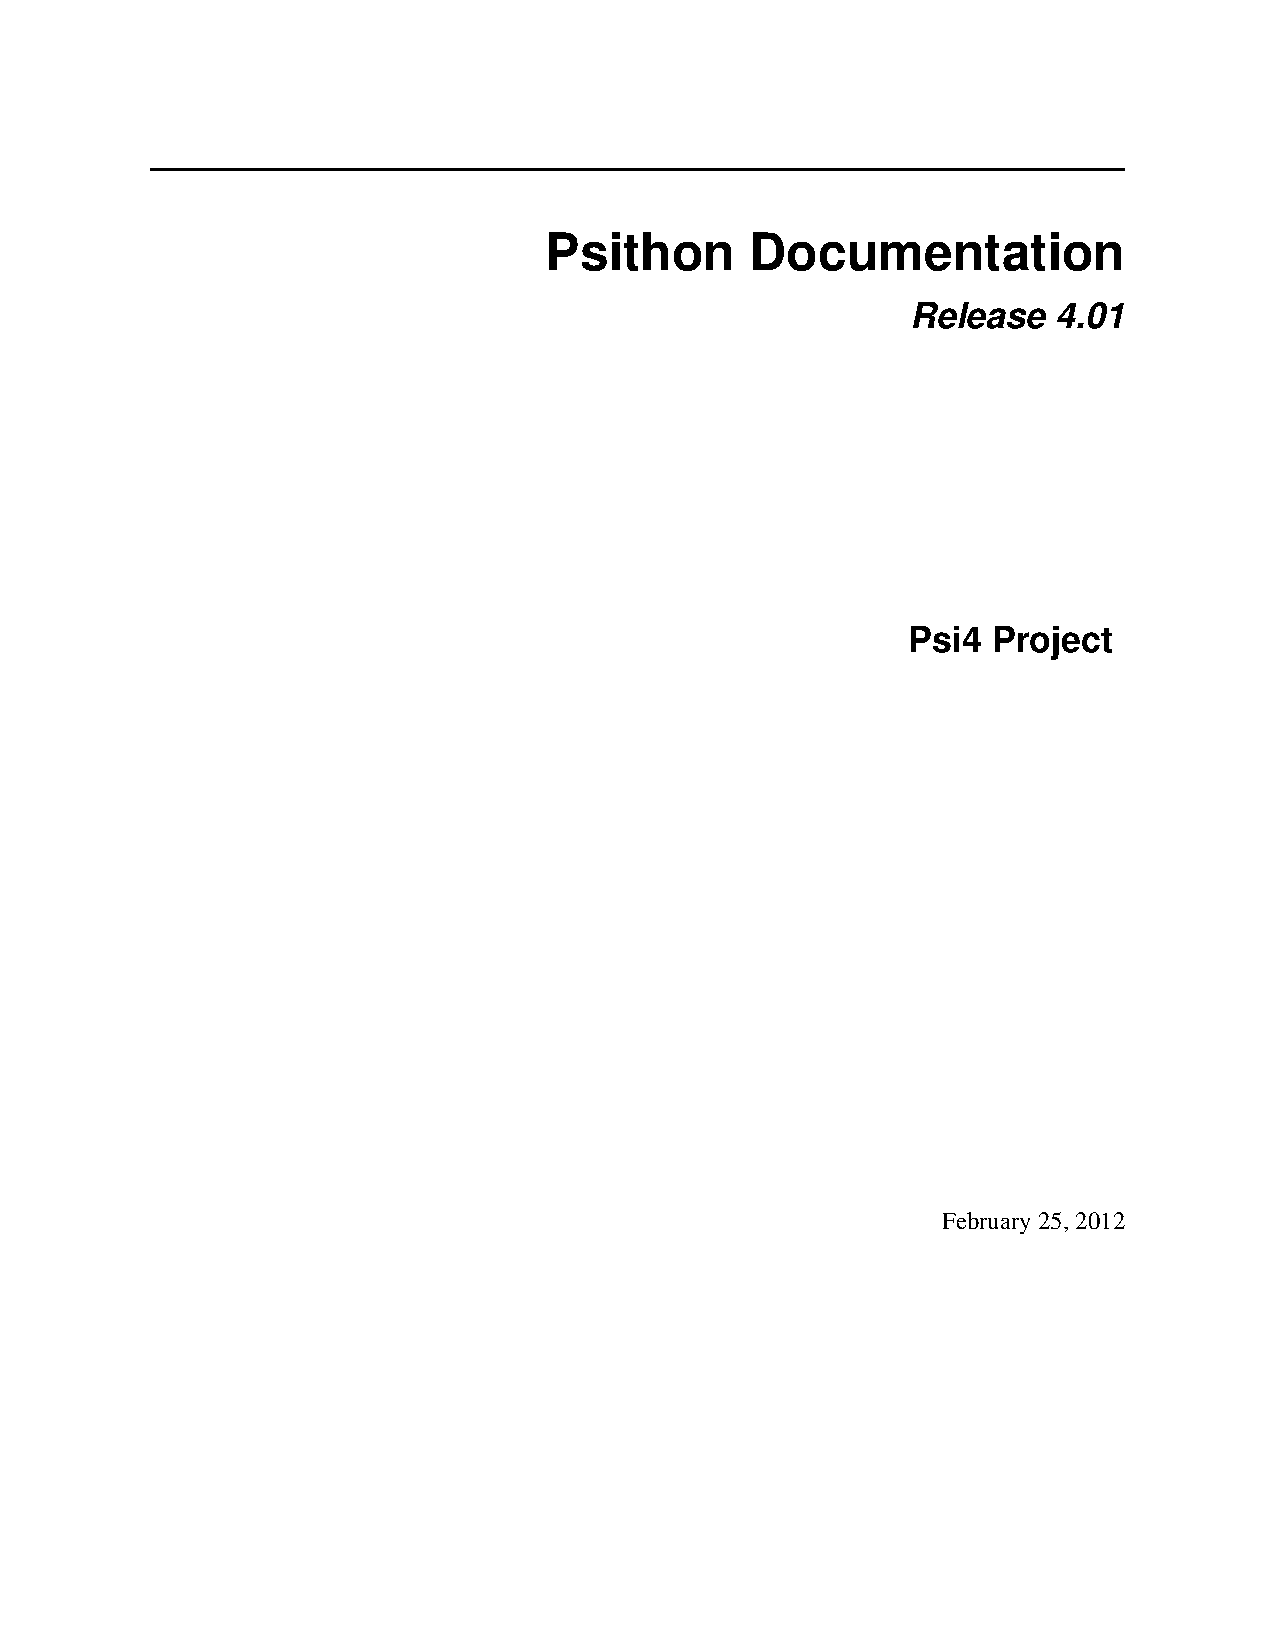
\includepdf[pages=-]{Psithon.pdf} 

\end{document}

